% =====================================================================
%  PRACA INŻYNIERSKA — SZKIC ROBOCZY (jeden plik)
%  "Sieci neuronowe do analizy rytmu oddechowego"
%  Maciej Łukasiewicz (197865) — Politechnika Gdańska
%  Promotor: dr hab. inż. Julian Szymański
%
%  Kompilacja:  tectonic praca_inzynierska.tex
%           lub  latexmk -pdf praca_inzynierska.tex
%
%  UWAGA: [TODO: ...] oznacza miejsca do uzupełnienia — usunąć makro
%  \todo przed oddaniem pracy.
% =====================================================================
\documentclass[12pt,a4paper,oneside]{report}

% Obsługa czcionek: działa zarówno pod XeLaTeX/tectonic, jak i pdfLaTeX
% (np. na Overleafie). Bez tego znaki diakrytyczne znikają z PDF-a.
\usepackage{iftex}
\ifPDFTeX
  \usepackage[utf8]{inputenc}
  \usepackage[T1]{fontenc}
  \usepackage{lmodern}
\else
  \usepackage{fontspec}
  \setmainfont{lmroman10-regular.otf}[
    BoldFont       = lmroman10-bold.otf,
    ItalicFont     = lmroman10-italic.otf,
    BoldItalicFont = lmroman10-bolditalic.otf]
  \setsansfont{lmsans10-regular.otf}[
    BoldFont   = lmsans10-bold.otf,
    ItalicFont = lmsans10-oblique.otf]
  \setmonofont{lmmono10-regular.otf}[
    BoldFont   = lmmonolt10-bold.otf,
    ItalicFont = lmmono10-italic.otf]
\fi
\usepackage[polish]{babel}
\usepackage[margin=2.5cm,bindingoffset=0.5cm]{geometry}
\usepackage{setspace}
\onehalfspacing

\usepackage{graphicx}
\graphicspath{{figures/}}
\usepackage{float}
\usepackage{subcaption}
\usepackage{booktabs}
\usepackage{longtable}
\usepackage{amsmath}
\usepackage{siunitx}
\sisetup{output-decimal-marker={,}}
\usepackage{xcolor}
\usepackage{tikz}
\setlength{\emergencystretch}{3em}  % ostatnia deska ratunku dla łamania akapitów
\usetikzlibrary{arrows.meta,positioning,fit,backgrounds}
\usepackage[hidelinks]{hyperref}

% Styl schematów blokowych potoku przetwarzania.
\tikzset{
  blok/.style   = {draw, rounded corners=2pt, align=center, font=\small,
                   minimum height=8mm, inner sep=4pt, fill=blue!5, draw=blue!45},
  wejscie/.style= {draw, rounded corners=2pt, align=center, font=\small,
                   minimum height=8mm, inner sep=4pt, fill=gray!10, draw=gray!55},
  wynik/.style  = {draw, rounded corners=2pt, align=center, font=\small,
                   minimum height=8mm, inner sep=4pt, fill=green!8, draw=green!45!black},
  strzalka/.style = {-{Latex[length=2mm]}, draw=gray!70},
}

% Znacznik miejsc do uzupełnienia (usunąć w wersji finalnej).
\newcommand{\todo}[1]{\textcolor{red!75!black}{\textbf{[TODO: #1]}}}
% Starsza nazwa zachowana dla istniejących odwołań; wszystkie rezerwy są
% celowo widoczne w PDF jako czerwone TODO.
\newcommand{\miejsce}[1]{\todo{#1}}

% Numery rysunków dwucyfrowych (np. 12.10) potrzebują szerszej kolumny
% w~spisie rysunków, aby podpis nie stykał się z~numerem.
\makeatletter
\renewcommand*\l@figure{\@dottedtocline{1}{1.5em}{3.0em}}
\makeatother

\title{Sieci neuronowe do analizy rytmu oddechowego}
\author{Maciej Łukasiewicz}
\date{Gdańsk 2026}

\begin{document}

% =====================================================================
% STRONA TYTUŁOWA
% =====================================================================
\begin{titlepage}
    \centering
    {\large Politechnika Gdańska\\[0.2em]
    Wydział Elektroniki, Telekomunikacji i Informatyki\par}
    \vspace{3.5cm}

    {\large Praca dyplomowa inżynierska\par}
    \vspace{1.2cm}
    {\LARGE\bfseries Sieci neuronowe do analizy\\[0.3em] rytmu oddechowego\par}
    \vspace{0.8cm}
    {\large\itshape Neural networks for respiratory rhythm analysis\par}
    \vspace{3cm}

    {\large Autor: Maciej Łukasiewicz (197865)\par}
    \vspace{0.4cm}
    {\large Promotor: dr hab. inż. Julian Szymański\par}
    \vfill
    {\large Gdańsk 2026\par}
    \vspace{0.5cm}
    {\footnotesize\todo{Zastąpić stronę tytułową wzorem z~MojaPG.}\par}
\end{titlepage}

% =====================================================================
% STRESZCZENIA
% =====================================================================
\chapter*{Streszczenie}
\addcontentsline{toc}{chapter}{Streszczenie}

Praca dotyczy bezkontaktowego pomiaru rytmu oddechowego i tętna przy użyciu
radaru. W ramach części implementacyjnej zbudowano dwa niezależne tory
pomiarowe: niskokosztowy radar dopplerowski HB100 (\SI{10.525}{GHz}) wraz
z zaprojektowanym od podstaw analogowym układem kondycjonowania sygnału oraz
radar impulsowo-koherentny Acconeer A121 (\SI{60}{GHz}) pracujący na surowych
danych Sparse~IQ. Opracowano algorytmy estymacji częstości oddechu i tętna
oparte na analizie fazy sygnału odbitego, aplikację desktopową do akwizycji
i podglądu na żywo oraz zestaw narzędzi do analizy offline. Przeprowadzono
równoczesne porównanie obu radarów: HB100 wykrywał obecność sterowanego
oddechu i~jego zatrzymanie w~powtarzanej serii do \SI{100}{cm} oraz
w~pojedynczym reteście \SI{150}{cm}. Dla pełnych, pogłębionych oddechów
estymator konsensusu harmonicznych HB100 w~12 blokach powtarzanej serii
\SIrange{30}{100}{cm} odtworzył zadany rytm \SI{0.20}{Hz} w~zakresie
\SIrange{0.198}{0.204}{Hz}. W~pojedynczym reteście \SI{150}{cm} uzyskano
\SI{0.190}{Hz} i~\SI{0.202}{Hz}, lecz z~małym marginesem jakości, dlatego
wynik traktowano jedynie jako wskazanie rytmu. Jednokanałowy przebieg nie
zachowywał stabilnie kierunku wdech--wydech; A121 umożliwiał taką analizę na
podstawie fazy I/Q. Przeprowadzono również
kontrolowany eksperyment porównujący trzy soczewki dielektryczne
(hiperboliczną, FZP i płaską pokrywę) oraz wpływ folii aluminiowej naklejonej
na klatkę piersiową (36 nagrań). W części eksperymentalnej system zastosowano
do całonocnego monitoringu snu, porównując wyniki z zegarkiem Garmin~Fenix~7.

\todo{Uzupełnić streszczenie o wyniki końcowe sieci neuronowych, gdy powstaną.}

\paragraph{Słowa kluczowe:} radar dopplerowski, radar impulsowo-koherentny,
rytm oddechowy, parametry witalne, HB100, Acconeer A121, analiza snu, sieci
neuronowe.

\clearpage
\chapter*{Abstract}
\addcontentsline{toc}{chapter}{Abstract}

\todo{Dodać streszczenie w~języku angielskim.}

\clearpage

% =====================================================================
\tableofcontents
\listoffigures
\listoftables

% =====================================================================
% WSTĘP
% =====================================================================
\chapter{Wstęp}

\section{Motywacja}
Rytm oddechowy i tętno należą do podstawowych parametrów opisujących stan
fizjologiczny człowieka. Ich długotrwała obserwacja jest istotna między innymi
w~medycynie snu, opiece domowej i~monitorowaniu osób, dla których zakładanie
klasycznych czujników może być uciążliwe. Pasy oddechowe, elektrody EKG
i~pulsoksymetry zapewniają bezpośredniejszy związek z~mierzoną wielkością, ale
wymagają kontaktu z~ciałem, właściwego założenia i~tolerowania przewodów lub
urządzenia nasobnego przez całą noc.

W~pracy rozpatrzono dwie grupy metod mniej typowych. Pierwszą stanowią radary,
które rejestrują ruch powierzchni ciała bez kontaktu i~nie zależą od oświetlenia.
Drugą są czujniki inercyjne: osobny moduł LSM6DS3 oraz sensory wbudowane
w~telefonie. IMU nie jest w~tej pracy wzorcem dla radaru, lecz niezależnym,
kontaktowym sposobem obserwowania kinematyki klatki piersiowej. Jego zaletą jest
niski koszt i~powszechna dostępność, szczególnie gdy akwizycję realizuje zwykły
smartfon. Badanie obejmuje zatem nie tylko dokładność estymowanej częstości, ale
również praktyczną użyteczność sygnału w~różnych pozycjach ciała.

Zestawienie prostego radaru CW HB100 z~koherentnym radarem impulsowym A121
pozwala pokazać, jak dostęp do odległości oraz zespolonych danych I/Q zmienia
możliwości analizy. Uzupełnieniem jest ocena wpływu soczewek, folii aluminiowej,
odzieży i~innych materiałów znajdujących się między radarem a~badanym.

\section{Cel i zakres pracy}
Celem głównym pracy jest zaprojektowanie i~ocena systemu do rejestracji oraz
analizy sygnałów związanych z~oddechem i~pracą serca z~wykorzystaniem
niekonwencjonalnych torów pomiarowych. Zakres obejmuje:
\begin{enumerate}
  \item budowę toru radaru dopplerowskiego HB100 wraz z~analogowym układem
  kondycjonowania i~akwizycją na ESP32,
  \item integrację radaru Acconeer A121 oraz analizę surowych danych Sparse~IQ,
  \item opracowanie algorytmów estymacji częstości oddechu i~tętna,
  \item uruchomienie osobnych torów inercyjnych: LSM6DS3 oraz aplikacji iOS
  wykorzystującej Core~Motion i~transmisję BLE,
  \item eksperymentalną ocenę wpływu odległości, soczewki, folii aluminiowej,
  materiałów pośrednich i~pozycji badanego na użyteczność sygnału,
  \item przygotowanie danych i~metod bazowych do oceny możliwości zastosowania
  sieci neuronowych w~analizie faz cyklu oddechowego.
\end{enumerate}
Ostateczny zakres części dotyczącej sieci neuronowych zostanie doprecyzowany po
ocenie jakości i~liczności zgromadzonego zbioru danych; nie wpływa to na zakres
zbudowanego systemu pomiarowego i~badań sygnałowych.

\section{Struktura pracy}
Praca dzieli się na trzy części:
\begin{itemize}
  \item \textbf{Część~\ref{part:sota}} --- przegląd literatury i istniejących
  rozwiązań bezkontaktowego pomiaru parametrów witalnych, ze szczególnym
  uwzględnieniem architektur radarowych.
  \item \textbf{Część~\ref{part:system}} --- opis zbudowanego systemu: tor
  radaru HB100 z autorskim front-endem analogowym, integracja radaru
  Acconeer~A121, osobne tory inercyjne, algorytmy estymacji oddechu i tętna
  oraz oprogramowanie. Po opisie metod przedstawiono kontrolowane porównanie
  HB100 z~A121, a~następnie eksperyment soczewek i~folii aluminiowej.
  \item \textbf{Część~\ref{part:eksperymenty}} --- zastosowanie systemu:
  całonocne pomiary snu, porównanie z zegarkiem Garmin~Fenix~7 oraz algorytmy
  klasyfikacji faz snu.
\end{itemize}

% =====================================================================
% =====================================================================
\part{Przegląd literatury i istniejących rozwiązań}
\label{part:sota}
% =====================================================================
% =====================================================================

\chapter{Bezkontaktowy pomiar parametrów witalnych}

\section{Mierzone parametry i ich zakresy fizjologiczne}
W~potoku przetwarzania przyjęto pasmo oddechowe
\SIrange{0.10}{0.50}{Hz}, odpowiadające 6--30 oddechom na minutę, oraz pasmo
sercowe \SIrange{0.70}{2.00}{Hz}, czyli 42--120 uderzeniom na minutę.
Oddychanie powoduje ruch powierzchni tułowia rzędu milimetrów, natomiast
drgania wywołane pracą serca są znacznie słabsze. Oba zjawiska mogą więc
pojawić się w~sygnale ruchowym, ale ich separacja wymaga innych filtrów i~miar
jakości.

Żaden z~zastosowanych czujników nie mierzy bezpośrednio objętości oddechowej
ani czynności elektrycznej serca. Radar obserwuje zmianę odległości radialnej
i~fazy odbicia, akcelerometr --- przyspieszenie właściwe, a~żyroskop ---
prędkość kątową obudowy. Częstość oddechu i~tętno są wielkościami wyznaczanymi
pośrednio z~okresowości tych sygnałów. Z~tego powodu wyniki należy interpretować
jako ocenę użyteczności metod ruchowych, a~nie jako walidację kliniczną.

\section{Motywacja kliniczna}
\miejsce{Polisomnografia jako złoty standard i jej ograniczenia. Monitoring
domowy, opieka senioralna, zespół nagłej śmierci łóżeczkowej.}

\section{Klasyczne metody kontaktowe}
Do metod klinicznych i~laboratoryjnych należą między innymi EKG,
pulsoksymetria, spirometria oraz pasy do pletyzmografii indukcyjnej (RIP).
Mierzą one inne wielkości fizyczne niż radar i~IMU, dlatego mogą pełnić rolę
zewnętrznego odniesienia, lecz nie są wymienne z~pomiarem ruchu powierzchni
ciała. W~niniejszym projekcie dane z~zegarka Garmin wykorzystano jedynie jako
porównanie konsumenckie dla pomiarów nocnych. LSM6DS3 i~iPhone są natomiast
pełnoprawnymi, osobnymi torami badanymi pod kątem wykrywalności oddechu i~tętna.

\chapter{Radarowe metody pomiaru parametrów witalnych}

\section{Radary dopplerowskie fali ciągłej (CW)}
Radar CW nadaje sinusoidę o~stałej częstotliwości. Ruch celu zmienia fazę
sygnału odbitego, a~ruch ze stałą prędkością powoduje przesunięcie Dopplera
$f_d=2v/\lambda$. Dla ruchu okresowego, takiego jak oddychanie, wyjście
mieszacza jest modulowane zmianą odległości powierzchni klatki piersiowej.
Układ jest prosty i~tani, ale sygnały od wszystkich obiektów w~wiązce sumują
się w~jednym kanale --- nie ma informacji, z~jakiej odległości pochodzi dany
składnik.

W~odbiorniku jednokanałowym napięcie ma w~uproszczeniu postać
\begin{equation}
  b(t)=A\cos\!\left(\frac{4\pi}{\lambda}[d_0+x(t)]+\varphi_0\right).
  \label{eq:cw-baseband}
\end{equation}
Znak fazy jest tu nieistotny: cosinus jest funkcją parzystą, więc przeciwna
konwencja zespolona daje ten sam przebieg po zmianie stałej $\varphi_0$.
Pojedynczy kanał rzeczywisty z~zasady nie niesie informacji o~znaku ruchu ---
i~właśnie stąd bierze się jego ograniczenie omawiane w~rozdziale
\ref{chap:hb100-a121-pomiar}.

Zależność~\eqref{eq:cw-baseband} nie jest liniowa względem przemieszczenia;
w~literaturze nosi ona nazwę \emph{nieliniowego efektu demodulacji fazy
Dopplera} \cite{boriclubecke2016}. Dla małego ruchu czułość zależy od fazy
statycznej celu: w~pewnych odległościach pochodna funkcji cosinus zanika
i~powstają punkty zerowe (\emph{null points}). Punkty optymalne i~zerowe
występują naprzemiennie co $\lambda/8$, więc już taka zmiana średniej
odległości celu przenosi układ z~maksimum czułości do minimum
\cite{mercuri2017}. Drugi, przesunięty o~$90^\circ$ kanał kwadraturowy Q
uzupełnia kanał I~i~pozwala śledzić fazę niezależnie od tego położenia;
demodulacja arcus tangens z~pary I/Q jest standardowym rozwiązaniem problemu
punktów zerowych \cite{park2007}. Korzyści z~toru kwadraturowego względem
odbiornika jednokanałowego opisano ilościowo już w~\cite{droitcour2004}.
Niskokosztowy HB100 udostępnia jednak tylko pojedyncze, rzeczywiste wyjście IF,
co stanowi jego fundamentalne ograniczenie \cite{hb100_doc}.

\section{Radary FMCW}
Radar FMCW nadaje ciąg odcinków, w~których częstotliwość nośna zmienia się
liniowo w~czasie (\emph{chirp}). Po zmieszaniu echa z~sygnałem nadawanym
częstotliwość różnicowa jest proporcjonalna do opóźnienia, a~więc do odległości
celu. FFT próbek pojedynczego chirpu tworzy profil odległości, natomiast analiza
faz kolejnych chirpów pozwala oszacować prędkość radialną. W~radarach
wielokanałowych dodatkowa analiza różnic faz między antenami dostarcza kąta
nadejścia. Cena za rozdzielczość odległościową to większa złożoność toru RF,
akwizycji i~obliczeń \cite{infineon_fmcw}.

\section{Radary impulsowo-koherentne (PCR)}
Radar impulsowo-koherentny wysyła krótkie impulsy i~próbkuje echo w~wybranych
opóźnieniach odpowiadających odległościom. Zachowanie koherencji pomiędzy
pomiarami umożliwia zwracanie zespolonych próbek I/Q. A121 pracuje w~paśmie
\SIrange{57}{64}{GHz}; przy długości fali około \SI{5}{mm} pełny obrót fazy
odpowiada zmianie drogi w~obie strony, czyli radialnemu przesunięciu celu
o~około \SI{2.5}{mm} \cite{acconeer_datasheet,acconeer_sparse_iq}.

A121 nie jest radarem FMCW i~nie wyznacza odległości z~częstotliwości dudnień
chirpu. Zarówno FMCW, jak i~PCR mogą wytworzyć profil celu względem odległości,
lecz robią to inną metodą: FMCW koduje opóźnienie w~częstotliwości sygnału IF,
a~PCR próbkuje odpowiedź na koherentny impuls. W~projekcie wykorzystywana jest
usługa Sparse~IQ: dla każdego punktu odległości zapisuje się amplitudę oraz
fazę odbicia.

\section{Radary UWB}
\miejsce{Ultra-wideband w monitoringu oddechu, rozdzielczość czasowa,
przegląd literatury.}

\section{Porównanie torów HB100 i A121}

Tabela~\ref{tab:hb100-a121} zestawia cechy istotne w~tej pracy. Nie jest to
porównanie dwóch równoważnych czujników: HB100 udostępnia minimalny tor
dopplerowski wymagający własnej elektroniki analogowej, natomiast A121 jest
zintegrowanym radarem koherentnym z~cyfrowym profilem odległości.

\begin{table}[H]
\centering
\caption{Porównanie radarów HB100 i Acconeer A121 na podstawie dokumentacji
producentów \cite{hb100_doc,acconeer_datasheet,waveshare_a121}.}
\label{tab:hb100-a121}
\small
\begin{tabular}{@{}p{3.1cm}p{5.25cm}p{5.25cm}@{}}
\toprule
Cecha & HB100 & Acconeer A121 / moduł Waveshare \\
\midrule
Pasmo pracy & \SI{10.525}{GHz}, $\lambda\approx\SI{28.5}{mm}$
& \SIrange{57}{64}{GHz}, $\lambda\approx\SI{5}{mm}$ \\
Rodzaj radaru & bistatyczny CW Doppler & impulsowo-koherentny PCR \\
Dane wyjściowe & jeden rzeczywisty sygnał analogowy IF & zespolone Sparse~IQ
dla wielu punktów odległości \\
Rozdzielenie celów po odległości & brak & tak, zależne od profilu impulsu \\
Mikroruch & zmiana napięcia zależna od fazy celu; punkty zerowe & zmiana fazy
I/Q w~wybranej bramce odległościowej \\
Typowy EIRP & 15~dBm & 11{,}4~dBm \\
Szerokość wiązki bez dodatkowej soczewki & $80^\circ$ w~azymucie,
$40^\circ$ w~elewacji & typowo $53^\circ$ w~płaszczyźnie E,
$65^\circ$ w~płaszczyźnie H \\
Elektronika zewnętrzna & wzmacniacz, filtr, ADC i~mikrokontroler & układ RF,
baseband i~anteny w~obudowie; moduł zawiera STM32 i~USB/UART \\
Najważniejsze ograniczenie w~projekcie & brak odległości i~kwadratury,
wrażliwość na całe otoczenie & większa złożoność konfiguracji, przeciek
bezpośredni, dobór profilu i~bramki celu \\
\bottomrule
\end{tabular}
\end{table}

\section{Odbicie, transmisja i tłumienie w materiałach}
\label{sec:materialy-radar}

Fala padająca na granicę materiałów dzieli się na część odbitą, transmitowaną
i~pochłoniętą. Proporcje zależą od zespolonej przenikalności elektrycznej,
przewodności, grubości, częstotliwości, polaryzacji i~kąta padania. Dlatego
potoczne stwierdzenie, że radar ,,widzi przez materiał'', jest nieprecyzyjne:
część energii może przejść przez przeszkodę, lecz po przejściu w~obie strony
i~odbiciu od klatki sygnał może już znaleźć się poniżej użytecznego poziomu.
Warstwowa budowa materiału może ponadto powodować interferencję i~zmieniać fazę
echa.

Różnica częstotliwości pomiędzy zastosowanymi radarami jest duża. Dla HB100
długość fali wynosi około \SI{28.5}{mm}, a~dla A121 około \SI{5}{mm}. Przy
krótszej fali większego znaczenia nabierają niewielkie nierówności powierzchni,
grubość warstw i~dokładne ustawienie. Pomiary materiałów budowlanych w~zakresie
\SIrange{4}{40}{GHz} wykazały dla wielu lekkich materiałów wewnętrznych jedynie
umiarkowaną stratę, podczas gdy pustaki powodowały straty większe o~dziesiątki
decybeli \cite{wallace2018}. W~badaniach budynków przy \SI{60}{GHz} zmierzono
zależne od kąta i~konstrukcji straty rzędu 12--32~dB dla ściany gipsowej,
8--18~dB dla szkła wewnętrznego i~26--41~dB dla drewnianych drzwi
\cite{jun2020}. Liczby te nie są stałymi materiałowymi --- obejmują konkretne
grubości, warstwy i~geometrię pomiaru --- ale pokazują, dlaczego wyników dla
\SI{10.525}{GHz} nie można bezpośrednio przenosić na \SI{60}{GHz}.

W~scenariuszu monitoringu snu szczególnie istotne są odzież i~pościel.
Eksperyment z~modulowanym reflektorem przy 61, 122 i~\SI{175}{GHz} wykazał, że
cienkie suche tkaniny wnoszą niewielką stratę, natomiast zawilgocenie może
znacznie zwiększyć tłumienie \cite{albrecht2023}. Uzasadnia to osobny test
przez suchą kołdrę, ale również wymaga zapisania rodzaju i~stanu materiału.

Metal zachowuje się odmiennie od dielektryków. Dla dobrego przewodnika energia
wnika jedynie na głębokość naskórkową
\begin{equation}
  \delta=\sqrt{\frac{2}{\omega\mu\sigma}}.
\end{equation}
Dla aluminium otrzymuje się w~przybliżeniu \SI{0.83}{\micro\metre} przy
\SI{10.525}{GHz} i~\SI{0.35}{\micro\metre} przy \SI{60}{GHz}, znacznie mniej
niż grubość folii kuchennej. Folia jest więc praktycznie nieprzezroczystym
reflektorem dla obu radarów. Nie oznacza to jednak automatycznej poprawy
pomiaru: niewielka łata konkuruje z~odbiciem od całego, bogatego w~wodę tułowia,
a~zmiana dominującego reflektora może jednocześnie zmienić amplitudę, fazę
i~wielodrogowość.

\section{Soczewki dielektryczne i kształtowanie wiązki}
\miejsce{Soczewki refrakcyjne (hiperboliczna, plano-convex) i dyfrakcyjne
(płytka strefowa Fresnela, FZP). Zysk anteny a szerokość wiązki, kompromis
zysk/pole widzenia. Materiał teoretyczny do wykorzystania w
rozdziale~\ref{chap:soczewki}.}

\chapter{Metody niradarowe}

\section{Czujniki inercyjne (IMU)}
Czujnik inercyjny umieszczony na tułowiu rejestruje zmianę orientacji i~ruch
wywołany oddechem. Składowe o~wyższej częstotliwości mogą zawierać drgania
sejsmokardiograficzne (SCG) i~gyro-kardiograficzne (GCG) związane z~pracą
serca. Jest to metoda kontaktowa, lecz nie wymaga specjalizowanego pasa
oddechowego: odpowiednie sensory znajdują się również w~telefonach.

Landreani i~wsp. rejestrowali oddech dwoma telefonami ułożonymi na mostku
i~nadbrzuszu osób leżących, stosując kontrolowane częstości
\SIrange{0.10}{0.25}{Hz}; po filtracji uzyskali błąd częstości poniżej 2\%
względem pasa, z~lepszymi wynikami nad brzuchem \cite{landreani2017}.
Nayak i~Bolic pokazali możliwość jednoczesnej estymacji oddechu i~tętna z~IMU
telefonu swobodnie leżącego na klatce w~pozycji na plecach
\cite{nayak2024}. Wyniki literaturowe uzasadniają sprawdzenie własnej aplikacji
iOS zarówno w~leżeniu, jak i~w~pozycji siedzącej, ale nie zastępują oceny
konkretnego telefonu, sposobu mocowania i~implementacji transmisji BLE.

W~projekcie zrealizowano dwa niezależne warianty: moduł LSM6DS3 odczytywany
przez ESP32 oraz aplikację iOS korzystającą z~Core~Motion. Oba zapisują trzy
osie akcelerometru i~żyroskopu do wspólnego formatu CSV, dzięki czemu można
porównać jakość przebiegu, stabilność częstości próbkowania i~wrażliwość na
pozycję ciała. Ich rola i~implementacja zostały opisane w~rozdziale
\ref{chap:imu}.

\section{Metody optyczne}
\miejsce{rPPG z kamery RGB, termowizja, kamery głębi.}

\section{Urządzenia nasobne jako źródło porównania}
\miejsce{Zegarki sportowe, w tym Garmin Fenix~7 wykorzystany jako konsumenckie
źródło porównania w części~\ref{part:eksperymenty}. Dokładność szacowania faz
snu przez zegarki względem polisomnografii.}

\section{Rozwiązania komercyjne}
\miejsce{Google Nest Hub (radar Soli), Withings Sleep Analyzer, Somnofy.}

\chapter{Uczenie maszynowe w analizie sygnałów oddechowych}
\label{chap:sota-ml}

\section{Klasyczne podejścia oparte na cechach}
\miejsce{FFT/Welch, filtracja pasmowa, detekcja pików --- czyli to, co
zaimplementowano jako baseline w rozdziale~\ref{chap:algorytmy}.}

\section{Sieci neuronowe dla sygnałów jednowymiarowych}
\miejsce{1D-CNN, LSTM/GRU, architektury typu transformer dla szeregów
czasowych; uczenie na spektrogramach.}

\section{Klasyfikacja faz oddechu}
\miejsce{Detekcja wdechu, wydechu i pauzy oddechowej --- przegląd metod.
To jest bezpośrednia podstawa teoretyczna dla rozdziału~\ref{chap:sieci}.}

\section{Dostępne zbiory danych}
\miejsce{Publiczne zbiory radarowych sygnałów witalnych; problem braku
etykiet faz oddechu i konieczność samodzielnej anotacji.}

% =====================================================================
% =====================================================================
\part{Zbudowany system pomiarowy}
\label{part:system}
% =====================================================================
% =====================================================================

\chapter{Architektura systemu i przebieg prac}
\label{chap:architektura}

\section{Ogólna architektura}
System składa się z czterech torów pomiarowych zintegrowanych w jednej
aplikacji desktopowej:
\begin{enumerate}
  \item radar dopplerowski HB100 z analogowym front-endem i akwizycją przez
  przetwornik ADC mikrokontrolera ESP32,
  \item radar impulsowo-koherentny Acconeer A121 podłączony przez USB-UART,
  dostarczający surowe dane Sparse~IQ,
  \item czujnik inercyjny LSM6DS3 na ESP32 (osobna metoda kontaktowa),
  \item aplikacja na iPhone strumieniująca dane z CoreMotion przez BLE
  (drugi wariant metody inercyjnej).
\end{enumerate}
Wspólna warstwa programowa zapewnia nagrywanie do plików CSV oraz bazy
SQLite, podgląd na żywo i analizę offline.

\miejsce{Rysunek blokowy całego systemu (do wykonania). Powinien pokazywać
przepływ: czujnik $\rightarrow$ kondycjonowanie $\rightarrow$ akwizycja
$\rightarrow$ zapis $\rightarrow$ analiza $\rightarrow$ wynik.}

\section{Przebieg prac i ewolucja projektu}
\label{sec:historia}

Projekt rozwijał się iteracyjnie; historia repozytorium dokumentuje kolejne
etapy oraz zmiany kierunku, które okazały się kluczowe dla ostatecznego
kształtu pracy.

\begin{table}[H]
\centering
\caption{Etapy realizacji projektu na podstawie historii repozytorium.}
\label{tab:historia}
\small
\begin{tabular}{@{}llp{7.6cm}@{}}
\toprule
Kolejność & Etap & Zakres prac \\
\midrule
1 & Start & Pierwsza akwizycja, uruchomienie toru radarowego HB100,
podstawowe wykresy i FFT. \\
2 & Tor IMU & Akwizycja I2C z LSM6DS3, analiza PCA, filtry
Butterwortha; wyodrębnienie rytmu oddechu i tętna. \\
3 & \emph{Zmiana kierunku} & Przeniesienie głównego nacisku
z~czujnika IMU na tor radarowy. \\
4 & Integracja A121 & Wsparcie dla radaru Acconeer~A121, schemat
front-endu analogowego, prototyp aplikacji. \\
5 & Parametry witalne & Poprawki algorytmu estymacji oddechu
i~tętna (bramkowanie odległościowe, miary pewności). \\
6 & Eksperymenty & Pomiary całonocne, aplikacja na iPhone, rozbudowa
bazy nagrań. \\
7 & Eksperyment sterowany & Automatyczna procedura badania soczewek
i~folii aluminiowej (36 nagrań, 12 warunków, 3 powtórzenia). \\
\bottomrule
\end{tabular}
\end{table}

Zmiana głównego kierunku z~IMU na radar wynikała z~odmiennego scenariusza
użytkowego: czujnik inercyjny musi poruszać się wraz z~ciałem, natomiast radar
umożliwia obserwację z~odległości. Nie oznacza to odrzucenia IMU ani nadania mu
roli wzorca. W~dalszej części oba warianty inercyjne są oceniane jako osobne,
niekonwencjonalne metody pomiaru. W~torach radarowych głównymi problemami były
niska amplituda analogowego wyjścia HB100, punkty zerowe odbiornika
jednokanałowego oraz wybór właściwego odbicia w~danych odległościowych A121.

% ---------------------------------------------------------------------
\chapter{Radar dopplerowski HB100}
\label{chap:hb100}

\section{Moduł HB100 --- zasada działania}
Moduł HB100 to niskokosztowy, bistatyczny radar dopplerowski fali ciągłej
pracujący nominalnie przy \SI{10.525}{GHz}. Odbity sygnał jest mieszany
z~sygnałem nadawanym, a~na wyjściu pośredniej częstotliwości (IF) pojawia się
składowa zależna od ruchu radialnego celu. Dla stałej prędkości $v$ przesunięcie
Dopplera wynosi
\begin{equation}
  f_d=\frac{2v}{\lambda}=\frac{2vf_0}{c}.
  \label{eq:hb100-doppler}
\end{equation}
Oddech jest jednak ruchem okresowym, a~nie ruchem ze stałą prędkością. Jego
przemieszczenie $x(t)$ zmienia fazę echa o~$4\pi x(t)/\lambda$, zgodnie
z~modelem~\eqref{eq:cw-baseband}. Przy $\lambda\approx\SI{28.5}{mm}$ pełny
obrót fazy odpowiada przesunięciu celu o~około \SI{14.2}{mm}. Ponieważ HB100
udostępnia tylko jeden rzeczywisty kanał IF, lokalna czułość na mały ruch jest
proporcjonalna do sinusa fazy statycznej. Punkty optymalne i~zerowe leżą
naprzemiennie co $\lambda/8$ \cite{mercuri2017}, więc zmiana średniej
odległości o~zaledwie $\lambda/8\approx\SI{3.6}{mm}$ może przenieść układ
z~maksimum czułości do punktu zerowego; kolejne punkty zerowe dzieli
$\lambda/4\approx\SI{7.1}{mm}$. W~pobliżu takiego punktu składowa podstawowa
oddechu słabnie, a~względnie rośnie druga harmoniczna. Nie jest to błąd
filtracji, lecz konsekwencja jednokanałowej architektury CW
\cite{droitcour2004}.

\begin{table}[H]
\centering
\caption{Wybrane parametry modułu HB100 według noty katalogowej
\cite{hb100_doc}.}
\label{tab:hb100-spec}
\small
\begin{tabular}{@{}p{5.7cm}p{7.0cm}@{}}
\toprule
Parametr & Wartość \\
\midrule
Częstotliwość nadawcza & \SIrange{10.520}{10.530}{GHz}, typowo
\SI{10.525}{GHz} \\
EIRP & \SIrange{12}{20}{dBm}, typowo \SI{15}{dBm} \\
Sygnał IF w~warunkach pomiarowych producenta & typowo
\SI{200}{\micro\volt} p-p przy dwukierunkowej stracie toru \SI{93}{dB} \\
Szum wyjścia IF & typowo \SI{5}{\micro\volt} RMS w~paśmie
\SIrange{10}{100}{Hz} \\
Szerokość wiązki & typowo $80^\circ$ w~azymucie i~$40^\circ$ w~elewacji \\
Zasilanie & \SI{5}{V}, pobór prądu \SIrange{30}{40}{mA} \\
\bottomrule
\end{tabular}
\end{table}

\section{Problem: amplituda sygnału wyjściowego}
Podstawowym problemem praktycznym okazała się bardzo niska amplituda sygnału
IF --- rzędu pojedynczych miliwoltów --- niemożliwa do bezpośredniego pomiaru
przetwornikiem ADC mikrokontrolera ESP32. Wymusiło to zaprojektowanie
dedykowanego analogowego układu kondycjonowania sygnału.

\section{Zaprojektowany analogowy front-end}
\label{sec:frontend}

Zbudowany układ (rys.~\ref{fig:hb100schemat}) opiera się na dwóch
symetrycznych stopniach nieodwracających na wzmacniaczu operacyjnym MCP6002.
Każdy stopień wykorzystuje $R_f = \SI{100}{k\ohm}$ oraz
$R_g = \SI{10}{k\ohm}$, co w~zakresie środkowym daje
\begin{equation}
  A_1=1+\frac{R_f}{R_g}=11,
  \qquad A_{1}A_{2}=121\;(\SI{41.7}{dB}).
  \label{eq:hb100-gain}
\end{equation}
Nie jest to jednak wzmocnienie stałe w~całym paśmie. Kondensator
\SI{22}{nF} równoległy do $R_f$ ogranicza dodatkowe wzmocnienie od góry,
a~kondensatory sprzęgające i~kondensatory w~gałęziach $R_g$ osłabiają je od
dołu. Wejścia sprzężone pojemnościowo
są podciągane do wirtualnej masy \SI{1.65}{V} rezystorami \SI{1}{M\ohm},
a~wyjście zabezpieczono rezystorem \SI{1}{k\ohm} przed wejściem ADC
(GPIO~33 / ADC1\_CH5). Zasilanie części analogowej realizuje stabilizator
liniowy MCP1700, aby odseparować ją od zakłóceń cyfrowych ESP32.

Dla wartości ze schematu częstotliwości narożne pojedynczych członów wynoszą
\begin{align}
  f_{HP,C}&=\frac{1}{2\pi R_{bias}C_{1,2}}
  =\frac{1}{2\pi\cdot\SI{1}{M\ohm}\cdot\SI{1}{\micro F}}
  \approx\SI{0.159}{Hz}, \\
  f_{HP,g}&=\frac{1}{2\pi R_gC_g}
  =\frac{1}{2\pi\cdot\SI{10}{k\ohm}\cdot\SI{100}{\micro F}}
  \approx\SI{0.159}{Hz}, \\
  f_{LP,f}&=\frac{1}{2\pi R_fC_f}
  =\frac{1}{2\pi\cdot\SI{100}{k\ohm}\cdot\SI{22}{nF}}
  \approx\SI{72.3}{Hz}.
  \label{eq:hb100-corners}
\end{align}
Pierwsza wartość dotyczy obu sprzężeń $C_1$ i~$C_2$ z~rezystorami
$R_{vbias}$, druga --- obu szeregowych gałęzi $R_g$--$C_g$, a~trzecia ---
obu kondensatorów w~sprzężeniu zwrotnym. Dwa człony o~tej samej wartości
granicznej nie są równoważne jednemu filtrowi pierwszego rzędu: ich tłumienia
sumują się.

Dokładniejszy model idealny jednego sprzężenia i~jednego stopnia ma postać
\begin{equation}
  \begin{aligned}
    H_C(s)&=\frac{sR_{bias}C}{1+sR_{bias}C}, &
    H_A(s)&=1+\frac{R_f/(1+sR_fC_f)}{R_g+1/(sC_g)}, \\
    H_{tot}(s)&=\left[H_C(s)H_A(s)\right]^2.&&
  \end{aligned}
  \label{eq:hb100-transfer}
\end{equation}
Z~tego modelu wynika maksimum około $120{,}3\times$ w~pobliżu
\SI{4}{Hz} oraz pasmo $-3$~dB względem tego maksimum około
\SIrange{0.36}{47.3}{Hz}. Przy częstości oddechu \SI{0.20}{Hz} wzmocnienie
wynosi około $45{,}6\times$ (\SI{33.2}{dB}), a~więc wyraźnie mniej niż
wartość środkowopasmowa $121\times$. Kondensatory $C_f$ nie tworzą przy tym
idealnego filtru dolnoprzepustowego o~wzmocnieniu dążącym do zera: dla bardzo
dużej częstotliwości stopień nieodwracający przechodzi w~wtórnik o~wzmocnieniu
bliskim jedności. Podane wartości są obliczeniami dla elementów idealnych,
niskiej impedancji źródła IF i~pominiętej tolerancji elementów; wymagają
potwierdzenia pomiarem charakterystyki gotowego prototypu.

\begin{figure}[H]
    \centering
    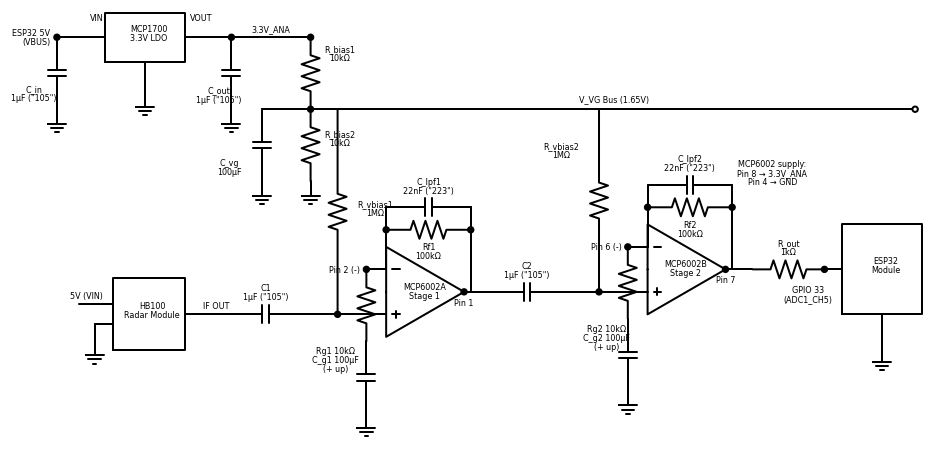
\includegraphics[width=0.95\textwidth]{hb100_frontend_schemat.png}
    \caption[Schemat analogowego front-endu HB100]{Schemat zaprojektowanego analogowego front-endu radaru HB100:
    dwa stopnie wzmacniające MCP6002 (do $\approx 121\times$),
    częstotliwościowo zależne wzmocnienie, wirtualna masa \SI{1.65}{V}
    i separowane zasilanie analogowe
    MCP1700.}
    \label{fig:hb100schemat}
\end{figure}

Wykonany prototyp przedstawiono na rys.~\ref{fig:hb100-stanowisko}. Moduł
HB100, analogowy układ kondycjonowania oraz ESP32 połączono na płytce
stykowej. Taka postać stanowiska ułatwiała zmianę elementów podczas
uruchamiania toru, ale wymagała zachowania stałego prowadzenia przewodów ze
względu na podatność wejścia o~małej amplitudzie na zakłócenia.

\begin{figure}[H]
    \centering
    \begin{subfigure}[t]{0.48\textwidth}
        \centering
        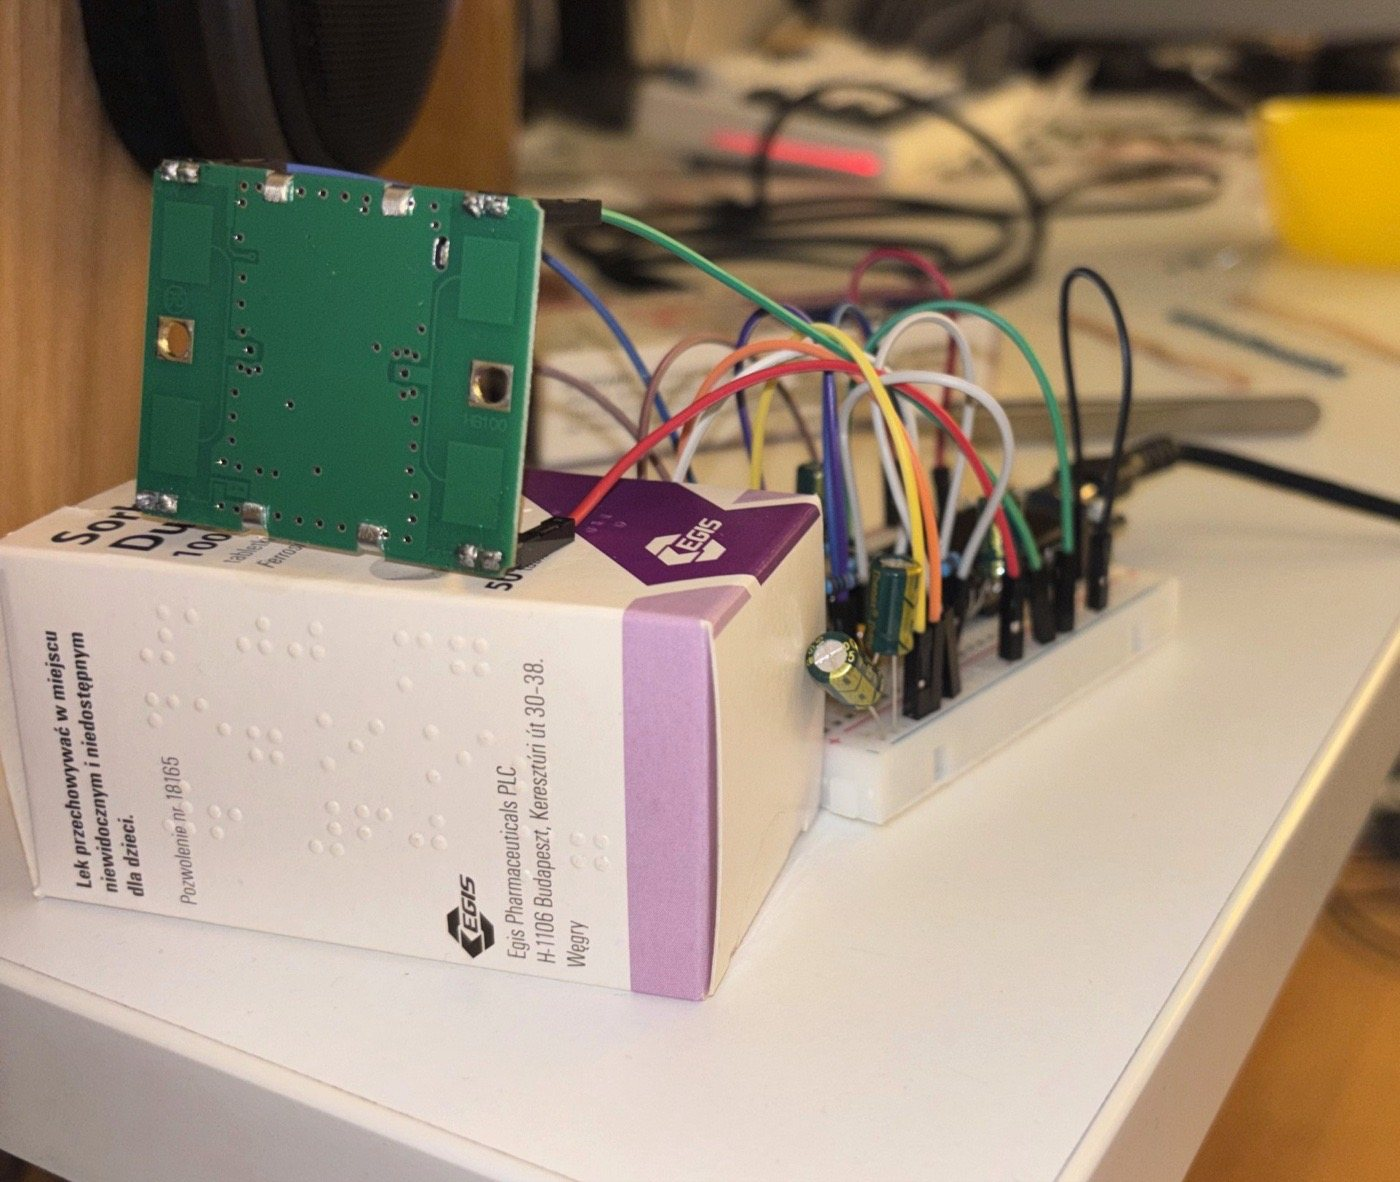
\includegraphics[width=\textwidth]{stanowisko_hb100.jpg}
        \caption{Moduł HB100 oraz układ kondycjonowania i~akwizycji.}
    \end{subfigure}
    \hfill
    \begin{subfigure}[t]{0.48\textwidth}
        \centering
        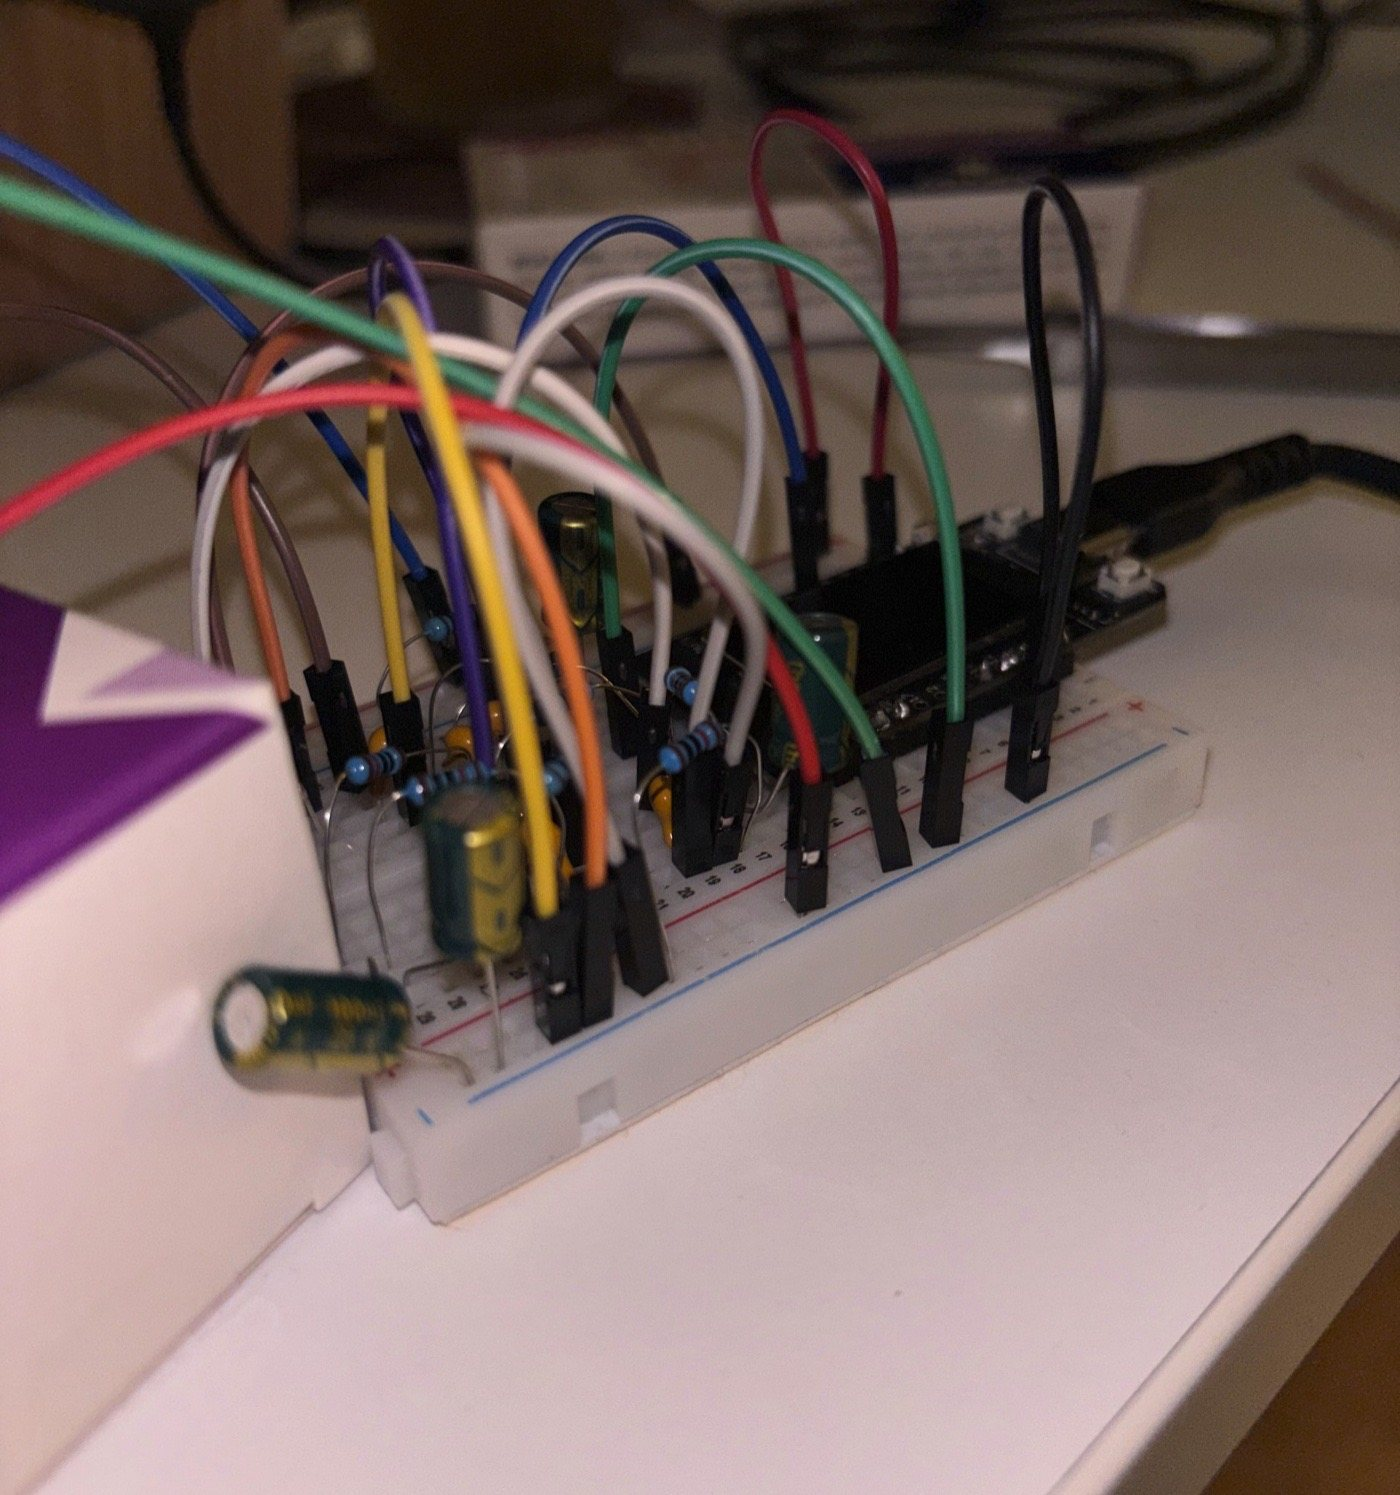
\includegraphics[width=\textwidth]{frontend_hb100.jpg}
        \caption{Zbliżenie analogowego front-endu na płytce stykowej.}
    \end{subfigure}
    \caption[Prototyp toru pomiarowego HB100]{Prototyp toru pomiarowego
    HB100 z~dwustopniowym front-endem i~mikrokontrolerem ESP32 (fotografie
    własne).}
    \label{fig:hb100-stanowisko}
\end{figure}

\miejsce{Do uzupełnienia pomiarowo: charakterystyka częstotliwościowa gotowego
układu, analiza szumów oraz pomiary oscyloskopem.}

\section{Akwizycja na ESP32}
Firmware w~katalogu \texttt{firmware/esp32\_radar\_adc} korzysta z~wejścia
GPIO~33 (ADC1, kanał~5) z~tłumieniem \texttt{ADC\_ATTEN\_DB\_12}. Każda
publikowana próbka jest średnią z~64 kolejnych konwersji ADC. Napięcie jest
przeliczane z~wykorzystaniem kalibracji liniowej ESP-IDF, a~w~razie jej braku
stosowane jest przeliczenie przybliżone. Zadany okres transmisji wynosi
\SI{4}{ms}, czyli nominalnie \SI{250}{Hz}; jest to duży nadmiar względem pasm
oddechu i~tętna, ale ułatwia późniejsze filtrowanie i~ocenę szumu toru.

Każdy wiersz transmisji przy \SI{230400}{baud} zawiera znacznik czasu z~zegara
\texttt{esp\_timer} w~milisekundach, uśredniony kod ADC oraz napięcie w~mV.
Na komputerze dane otrzymują nagłówek
\texttt{Timestamp\_ms,RawADC,Voltage\_mV}. O~rzeczywistej częstości próbkowania
nie należy jednak wnioskować wyłącznie z~wartości zadanej: średni czas 64
konwersji, formatowanie tekstu i~transmisja mogą powodować jitter. Dlatego jest
ona wyznaczana z~różnic znaczników czasu, a~przed każdym eksperymentem należy
sprawdzić monotoniczność czasu, liczbę brakujących próbek oraz rozkład odstępów.
Szybkość \SI{230400}{baud} zastąpiła wcześniejsze \SI{921600}{baud}, przy
których zastosowany konwerter USB--UART i~sterownik WCH w~systemie macOS nie
zwracały niezawodnie czystego tekstu. W~\SI{12}{s} próby kontrolnej po
przeprogramowaniu odebrano 3003 surowe ramki ASCII, co odpowiada
\SI{250.0}{Hz}; nie zastosowano korekcji transportu, nie odrzucono żadnego
wiersza i~nie stwierdzono nasycenia przetwornika ADC.

Podczas pomiarów tor HB100 i~ESP32 były zasilane z~portu USB laptopa
pracującego na akumulatorze; zasilacz laptopa pozostawał odłączony od sieci.
Usuwało to bezpośrednią drogę przewodzenia przydźwięku z~zasilania
\SI{230}{V}/\SI{50}{Hz} przez ładowarkę i~przewód USB. Nie oznacza jednak
całkowitego wyeliminowania składowej \SI{50}{Hz}: może ona nadal sprzęgać się
elektromagnetycznie z~instalacji pomieszczenia, a~w~torze mogą występować także
zakłócenia cyfrowe i~szum przetwornicy laptopa. Warunek zasilania bateryjnego
ogranicza więc jedno istotne źródło zakłóceń, lecz nie zastępuje pomiaru widma
tła.


\section{Ograniczenia toru HB100 i wnioski}
HB100 sumuje echa ze wszystkich obiektów w~wiązce, nie rozdziela ich po
odległości i~nie udostępnia kanału kwadraturowego. Wynik zależy więc od
statycznej fazy celu, ruchu tła i~wielodrogowości. Te ograniczenia wyjaśniają,
dlaczego nawet duże wzmocnienie analogowe nie gwarantuje powtarzalnego pomiaru
mikroruchu. HB100 pozostaje jednak samodzielną niskokosztową metodą oraz
demonstracją kompletnego łańcucha inżynierskiego --- od mikrofalowego modułu
i~analogowego kondycjonowania po cyfrową analizę. Na poziomie konstrukcyjnym
nie można jeszcze przesądzić, które informacje oddechowe pozostają użyteczne:
osobno trzeba ocenić wykrycie ruchu, jego okresowość oraz kierunek fazy cyklu.
Taką ocenę przedstawiono dopiero po opisie A121 i~algorytmów, w~rozdziale
\ref{chap:hb100-a121-pomiar}.

% ---------------------------------------------------------------------
\chapter{Radar impulsowo-koherentny Acconeer A121}
\label{chap:a121}

\section{Charakterystyka czujnika}
Acconeer A121 to radar impulsowo-koherentny pracujący w~paśmie
\SIrange{57}{64}{GHz} \cite{acconeer_datasheet}.
W~przeciwieństwie do HB100 dostarcza on zespolone dane Sparse~IQ dla całego
szeregu bramek odległościowych, co pozwala jednocześnie \emph{zlokalizować}
cel i~śledzić \emph{fazę} sygnału od niego odbitego. Przy długości fali
$\lambda \approx \SI{5}{mm}$ przesunięcie fazy $\Delta\varphi$ odpowiada
przemieszczeniu celu
\begin{equation}
    \Delta d = \frac{\lambda}{4\pi}\,\Delta\varphi ,
    \label{eq:faza}
\end{equation}
co daje czułość rzędu ułamków milimetra --- wystarczającą, aby zarejestrować
zarówno oddech (kilka milimetrów), jak i~składową sercową. Konwencję znaku
w~równaniu~\eqref{eq:faza} omówiono w~sekcji~\ref{sec:model-sygnalu}; jest ona
stałą właściwością toru, dzięki czemu faza A121 niesie nie tylko wielkość, lecz
także \emph{kierunek} ruchu klatki.

Sam układ A121 integruje część radiową, baseband oraz anteny w~obudowie
o~wymiarach około $5{,}2\times5{,}5\times0{,}88$~mm. Producent podaje EIRP
\SI{11.4}{dBm}, typowe szerokości wiązki $53^\circ$ i~$65^\circ$ w~dwóch
płaszczyznach oraz możliwość bezwzględnego pomiaru odległości do \SI{23}{m},
zależną od celu i~konfiguracji \cite{acconeer_datasheet}. Ostatnia wartość nie
jest zasięgiem detekcji oddechu; mikroruch klatki stanowi znacznie trudniejszy
cel i~musi zostać scharakteryzowany eksperymentalnie.

W~projekcie użyto płytki Waveshare A121 Range Sensor z~mikrokontrolerem
STM32L431, interfejsem USB/UART oraz zasilaniem \SI{5}{V}. Moduł ma wymiary
$39\times39$~mm i~według producenta pobiera maksymalnie \SI{80}{mA}
\cite{waveshare_a121}. Rozdzielczości profilu odległościowego nie należy mylić
z~czułością fazową: dla profilu~3 szerokość odpowiedzi impulsowej jest rzędu
\SI{89}{mm}, lecz po ustabilizowaniu właściwej bramki względną zmianę drogi
można śledzić znacznie dokładniej na podstawie fazy.

\section{Konfiguracja pomiarowa}
W~pomiarach wykorzystano konfigurację: profil~3, HWAAS~32, 8~przemiatań na
ramkę, częstotliwość ramek \SI{20}{Hz}, zakres \SIrange{0.20}{1.50}{m}.
Dane zapisywane są do plików CSV zawierających m.in. składowe rzeczywistą
i~urojoną dla każdej bramki odległościowej, amplitudę, fazę oraz metadane
z~wbudowanych detektorów Acconeera.

Profil~3 stanowi kompromis między energią impulsu, separacją celów i~zasięgiem.
Parametr HWAAS określa liczbę sprzętowo uśrednianych próbek: jego zwiększenie
poprawia SNR kosztem czasu pomiaru i~zużycia energii. Osiem przemiatań jest
uśrednianych w~ramce, natomiast \SI{20}{Hz} zachowuje duży zapas względem pasma
oddechu oraz pasma sercowego używanego w~projekcie. Dla każdego dystansu trzeba
rozszerzyć konfigurowany przedział tak, aby obejmował cel; w~przeciwnym razie
eksperyment mierzy ograniczenie konfiguracji, a~nie radaru. Komputer łączy się
z~czujnikiem przez klienta szeregowego Acconeer Exploration Tool. Z~każdej
ramki zapisywane są odległości oraz tablice wartości rzeczywistych i~urojonych,
co umożliwia ponowne wykonanie całej analizy offline.

% ---------------------------------------------------------------------
\chapter{Inercyjne tory pomiarowe}
\label{chap:imu}

Czujniki inercyjne tworzą w~tej pracy osobny nurt pomiarowy. Rejestrują ruch
obudowy spoczywającej na tułowiu, podczas gdy radar rejestruje zmianę drogi
propagacji fali. Zgodność częstości wyznaczonej z~obu metod może być użyteczną
kontrolą spójności, ale sama nie czyni IMU wzorcem dla radaru. Pierwszy test
ograniczono do najprostszego wariantu: pomiaru w~pozycji na plecach. Jego celem
jest sprawdzenie, czy oba tory dają czytelny sygnał oddechowy; uogólnienie na
inne postawy wymaga osobnych danych.

\section{Moduł LSM6DS3 z ESP32}
LSM6DS3 zawiera trójosiowy akcelerometr i~trójosiowy żyroskop. Wykorzystany
firmware ESP-IDF komunikuje się z~czujnikiem po I2C z~częstotliwością
\SI{400}{kHz}. Rejestry \texttt{CTRL1\_XL} oraz \texttt{CTRL2\_G} otrzymują
wartość \texttt{0x40}, co ustawia nominalną częstotliwość ODR obu sensorów na
\SI{104}{Hz}, zakres akcelerometru $\pm2g$ i~żyroskopu
$\pm\SI{250}{\degree\per\second}$ \cite{lsm6ds3}. Częstotliwość dobrano do
pasma oddechowego zamiast stosować niepotrzebne \SI{1.66}{kHz}. Po zgłoszeniu
gotowości obu części odczytywane są jednym odczytem I2C trzy osie
przyspieszenia w~$g$ oraz trzy osie prędkości kątowej w~stopniach na sekundę.
Każdy wiersz UART zawiera dodatkowo licznik próbki i~czas
\texttt{esp\_timer} w~mikrosekundach; pętla firmware utrzymuje rzeczywistą
częstotliwość około \SI{100}{Hz}.

\begin{figure}[H]
    \centering
    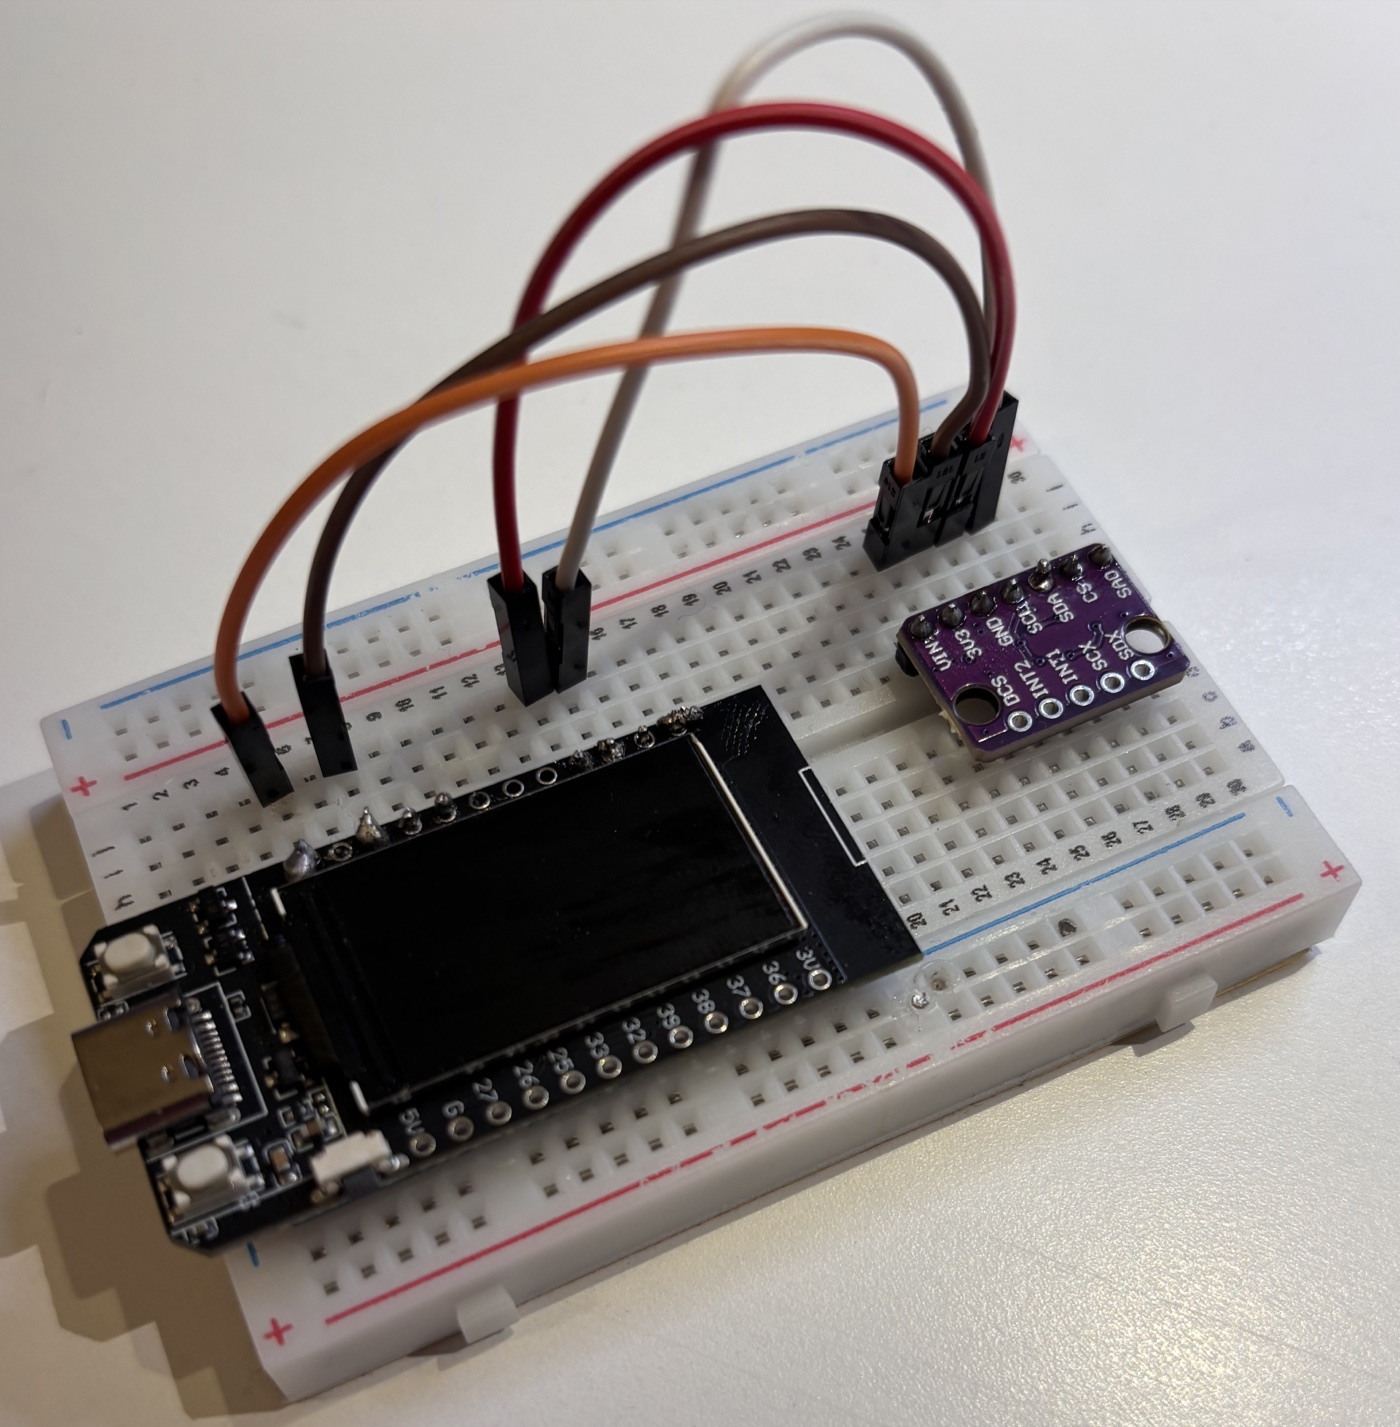
\includegraphics[width=0.68\textwidth]{stanowisko_lsm6ds3.jpg}
    \caption[Stanowisko pomiarowe z~modułem LSM6DS3]{Moduł LSM6DS3 połączony
    przez I2C z~mikrokontrolerem ESP32 na prototypowej płytce stykowej
    (fotografia własna).}
    \label{fig:lsm6ds3-stanowisko}
\end{figure}

\subsection{Przetwarzanie sygnału IMU}

Analiza offline filtruje trzy osie w~paśmie oddechowym
\SIrange{0.10}{0.60}{Hz}, a~następnie wyznacza pierwszą składową główną PCA.
Osobna ścieżka łączy żyroskop z~kierunkiem grawitacji filtrem komplementarnym
i~tworzy sygnał kąta oddechowego. Składowa sercowa jest poszukiwana w~paśmie
\SIrange{0.65}{4.00}{Hz}. PCA redukuje zależność od wyboru pojedynczej osi,
ale nie gwarantuje niezmienności względem postawy, miejsca położenia czujnika
ani przesunięcia podczas pomiaru. W~serii podstawowej nie testuje się tej
niezmienności: urządzenia pozostają w~stałej orientacji na klatce osoby
leżącej na plecach.

Nie jest to drugi, niezależny algorytm rekonstrukcji fizycznego
przemieszczenia porównywalny z~torem fazowym A121. PCA jest tu celowym,
prostym połączeniem trzech osi akcelerometru w~jeden przebieg diagnostyczny;
znak jego składowej jest umowny. Dalsza ocena ogranicza się więc do
wykrywalności rytmu, zaniku ruchu podczas wstrzymania oraz zgodności z~rytmem
zadającym, a~nie do bezwzględnego przypisania fazy wdech--wydech.

\section{Aplikacja iOS i transmisja BLE}
Aplikacja \emph{RespiPhoneIMU} korzysta z~\texttt{CMDeviceMotion}. Użytkownik
wybiera \SI{25}{Hz}, \SI{50}{Hz} albo \SI{100}{Hz}; domyślnie ustawiono
\SI{100}{Hz}. Zapisywane przyspieszenie jest sumą wektora grawitacji
i~\texttt{userAcceleration}, natomiast prędkość kątowa pochodzi z~estymaty
\texttt{rotationRate} dostarczanej przez Core~Motion \cite{apple_coremotion}.
Każda próbka otrzymuje znacznik \texttt{motion.timestamp} względem początku
strumienia. Jest to istotne, ponieważ Apple zaleca wyznaczanie rzeczywistych
odstępów aktualizacji właśnie ze znaczników czasu, a~nie z~samej zadanej
wartości interwału \cite{apple_coremotion_interval}.

Telefon działa jako urządzenie peryferyjne BLE. W~jednym powiadomieniu może
przesłać kilka próbek; każda zawiera własny czas, sześć składowych ruchu,
a~nagłówek paczki --- numer sekwencyjny. Komputer wyrównuje pierwszy czas
telefonu do zegara hosta i~zapisuje ten sam schemat CSV co dla LSM6DS3:
\texttt{Time\_ms,ax,ay,az,gx,gy,gz}. Grupowanie próbek w~paczki nie zniekształca
więc osi czasu, o~ile zachowane są czasy próbek. Numer sekwencyjny umożliwia
wykrywanie zagubionych powiadomień po dodaniu kontroli jego ciągłości po
stronie odbiornika.

\begin{figure}[H]
    \centering
    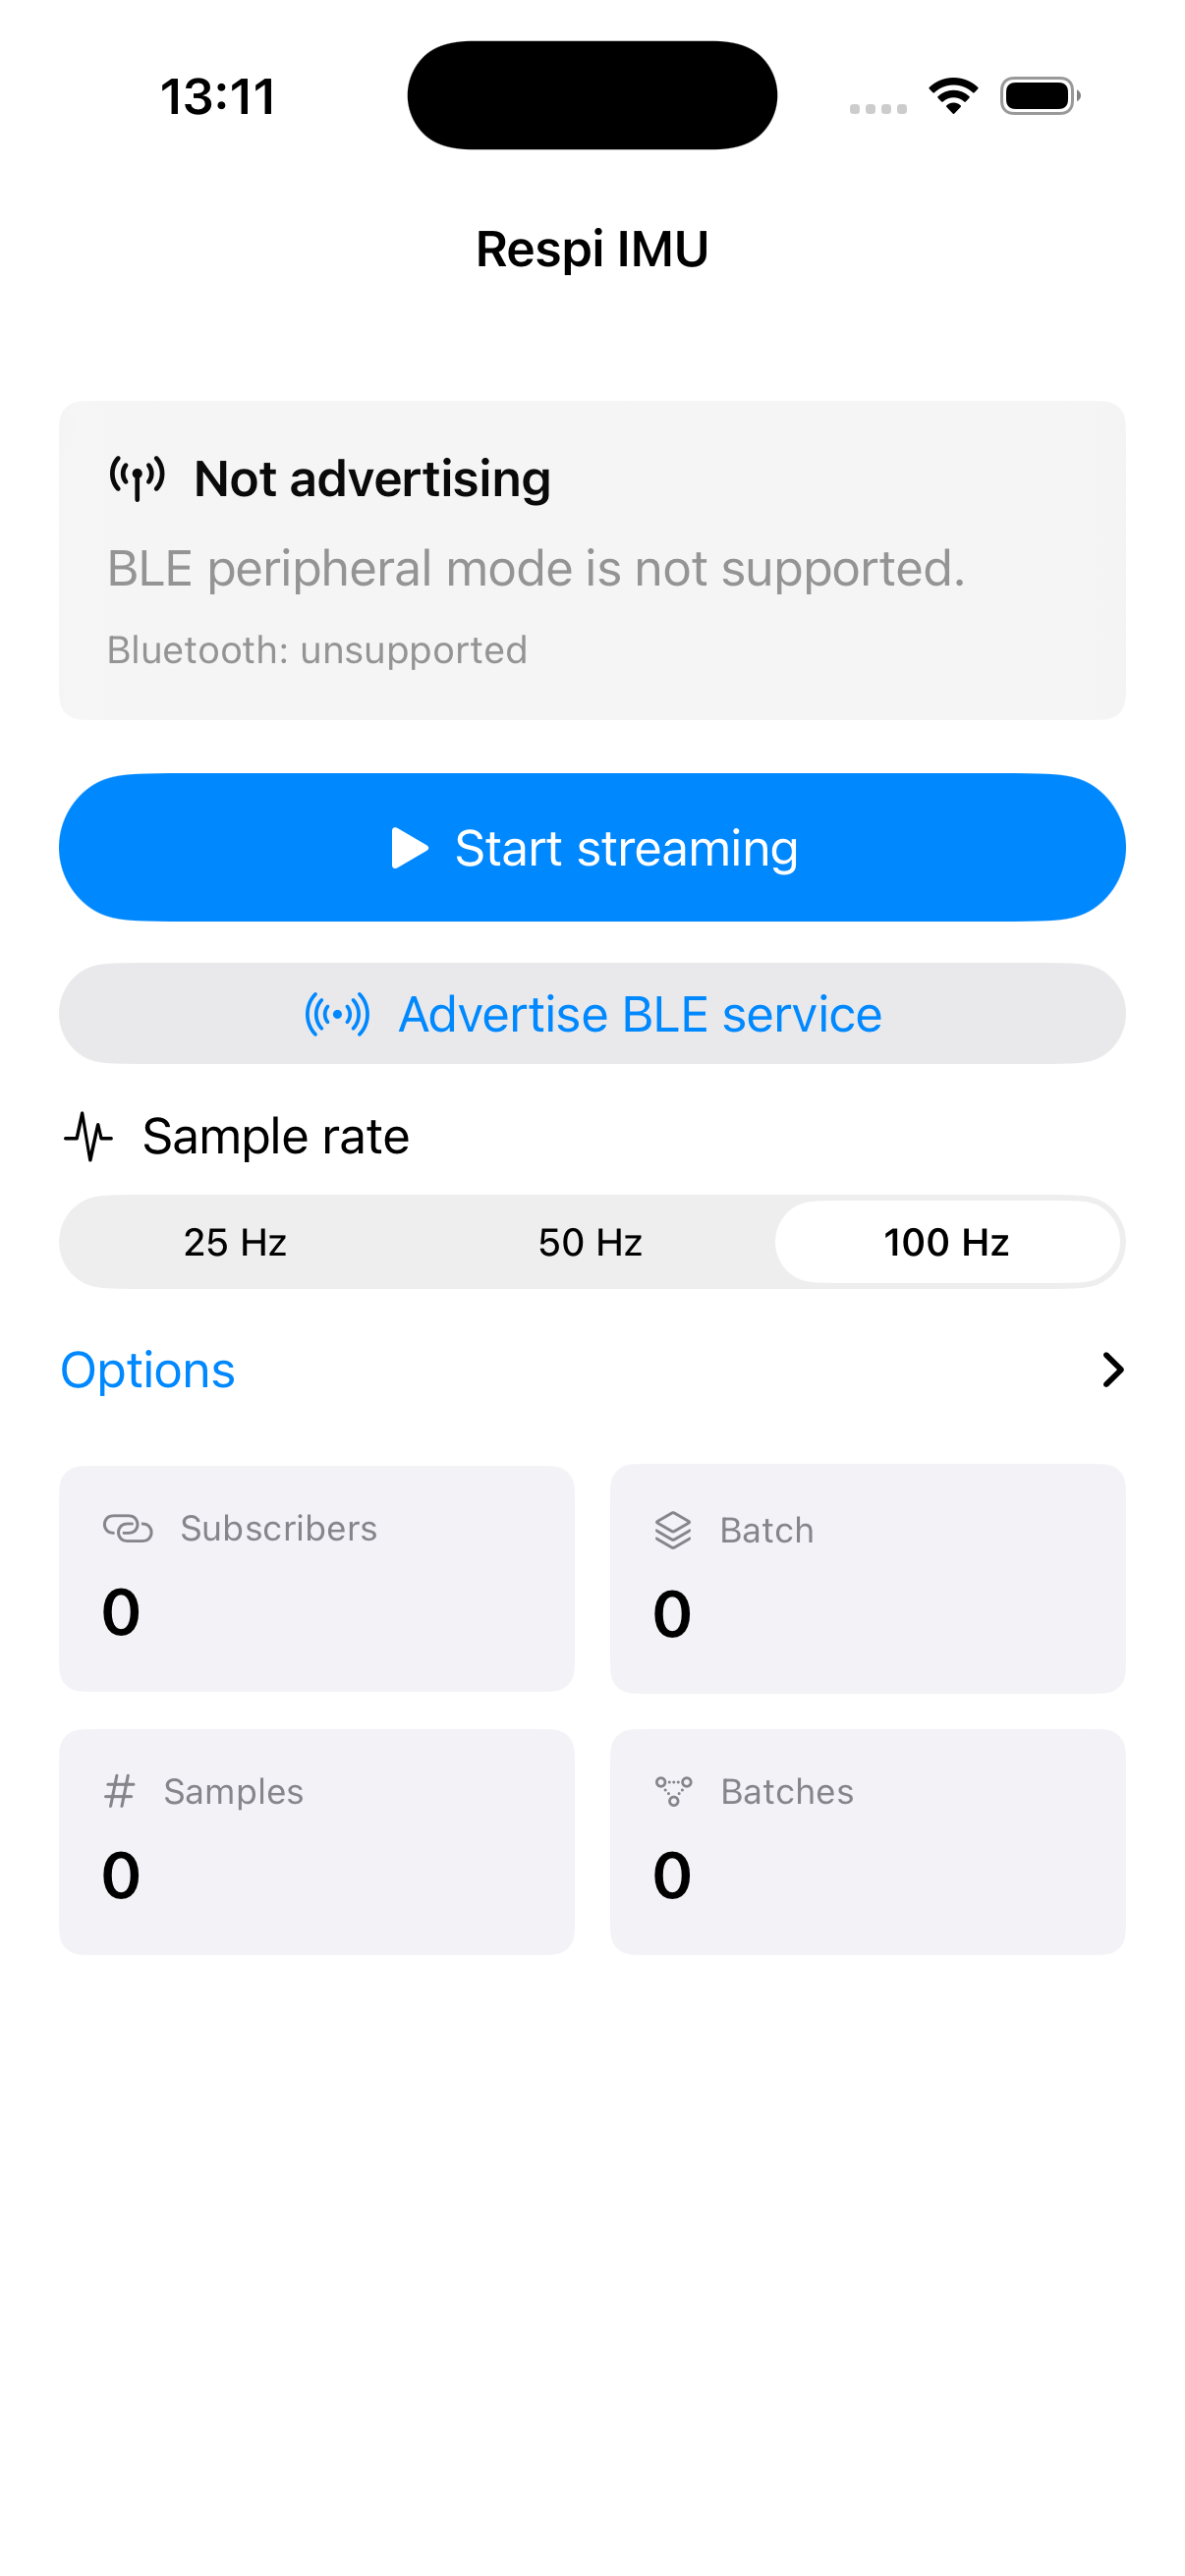
\includegraphics[width=0.34\textwidth]{respi_iphone_ble_ui.png}
    \caption[Interfejs aplikacji iOS RespiPhoneIMU]{Aplikacja
    \emph{RespiPhoneIMU}: wybór częstotliwości \SI{25}{Hz}, \SI{50}{Hz} lub
    \SI{100}{Hz}, sterowanie reklamowaniem usługi BLE i~liczniki transmisji.
    Zrzut wykonano w~symulatorze iOS, który poprawnie prezentuje interfejs,
    lecz nie obsługuje trybu peryferyjnego BLE; widoczny stan
    \emph{unsupported} nie jest wynikiem testu telefonu fizycznego.}
    \label{fig:iphone-ble-ui}
\end{figure}

\section{Synchronizacja i kryteria oceny}
Aktualna wersja firmware LSM6DS3 wysyła dla każdej próbki licznik oraz czas
\texttt{esp\_timer} w~mikrosekundach przed sześcioma wartościami ruchu. Plik
CSV zachowuje zarówno ten czas urządzenia, jak i~czas nadejścia na hoście;
umożliwia to wyznaczenie rzeczywistej częstotliwości oraz dokładne policzenie
luk i~duplikatów na podstawie licznika. iPhone przekazuje własne czasy próbek,
a~nagłówek paczki BLE zawiera numer sekwencyjny. Po stronie odbiornika
rejestrowane są niepoprawne, brakujące i~zduplikowane paczki oraz resety
numeracji.

Do równoczesnych pomiarów obu IMU przygotowano osobny skrypt z~wspólną osią
czasu komend, plikami CSV obu urządzeń, plikiem komend i~manifestem. Przerwana
albo odrzucona próba usuwa wyłącznie pliki bieżącego nagrania. Przed analizą
ilościową skrypt sprawdza rzeczywistą liczbę próbek na sekundę, liczbę
utraconych próbek oraz pokrycie całego okna czasowego. Jest to potrzebne,
ponieważ krótka, lokalnie regularna paczka BLE może mieć poprawne $\Delta t$,
a~mimo to nie obejmować prawie całej próby. Zapis iPhone jest akceptowany
tylko wtedy, gdy pokrywa co najmniej 95\% oczekiwanych próbek i~czasu próby,
a~najdłuższa luka nie przekracza \SI{0.25}{s}.

Podstawowy eksperyment obejmował dla obu urządzeń wyłącznie leżenie na plecach,
oddech swobodny, oddech narzucony programowym przewodnikiem oraz krótki odcinek
wstrzymania oddechu; każdy wariant powtarzano dwukrotnie. Zapisy obu torów
oceniono trzema miarami, wyznaczonymi tą samą filtracją pasmową i~tym samym
PCA trzech osi przyspieszenia:
\begin{itemize}
  \item \textbf{dominująca częstość $f_R$} --- położenie maksimum widma
  w~paśmie oddechowym, porównywane z~rytmem zadanym przez przewodnika;
  \item \textbf{czytelność piku $Q_{\mathrm{spec}}$} --- stosunek najwyższego
  piku widma do mediany pozostałej części pasma oddechowego, w~dB. Celowo nie
  nazwano jej SNR: mianownik jest tłem widmowym w~paśmie oddechu, a~nie
  skalibrowanym szumem toru pomiarowego;
  \item \textbf{zgodność z~komendami $|\rho_{\mathrm{cue}}|$} --- bezwzględna
  korelacja pochodnej przebiegu PCA z~naprzemiennymi komendami wdechu
  i~wydechu po dopasowaniu czasowym.
\end{itemize}
Osobno raportowany jest iloraz RMS ostatnich \SI{10}{s} wstrzymania do RMS
odcinka oddechowego, sprawdzający, czy rejestrowany ruch faktycznie zanika po
zatrzymaniu oddechu.

Wnioski dotyczą użyteczności każdego toru z~osobna, a~nie jego zgodności
z~rzekomym wzorcem radarowym. Miary są celowo skromne: opisują wykrywalność
rytmu i~jego zanik, a~nie bezwzględną amplitudę, znak ani fazę PCA, których nie
interpretuje się fizycznie. Wyniki obu serii przedstawiono w~sekcjach
\ref{sec:imu-lsm6ds3-test} i~\ref{sec:imu-iphone-porownanie}.

\todo{Po potwierdzeniu użyteczności w~leżeniu wykonać eksperyment
w~pozycji siedzącej. Następnie, jeśli zakres pracy na to pozwoli, sprawdzić
leżenie na boku, różne miejsca i~orientacje telefonu oraz odporność PCA na
zmianę postawy.}

\section{Test LSM6DS3 na klatce piersiowej}
\label{sec:imu-lsm6ds3-test}

Wykonano cztery próby w~pozycji na plecach. Moduł LSM6DS3 zamocowano na
wysokości sutków, na górnej części klatki piersiowej; podczas całej serii jego
położenie i~orientacja pozostawały stałe. Dwie próby trwały \SI{60}{s}:
\SI{10}{s} uspokojenia pozycji, \SI{35}{s} oddechu swobodnego i~\SI{15}{s}
wstrzymania po wydechu. Dwie kolejne trwały \SI{90}{s}: po \SI{10}{s}
oddechu swobodnego badany wykonał 7~cykli wdech \SI{2}{s} / wydech
\SI{3}{s}, \SI{15}{s} wstrzymania, a~następnie 6~dalszych cykli o~tym samym
rytmie. W~częściach sterowanych zadana częstość wynosiła zatem
12~oddechów/min.

W~każdej próbie odebrano ciągły, znacznikowany strumień LSM6DS3 z~zerową
liczbą luk licznika, duplikatów, resetów i~niepoprawnych wierszy UART.
Tabela~\ref{tab:imu-lsm-wyniki} przedstawia częstotliwość dominującą z~PCA
przyspieszeń. W~dwóch próbach sterowanych wynik wyniósł 11,99~oddechów/min,
czyli praktycznie dokładnie wartość zadaną. W~próbach oddechu swobodnego
uzyskano 12,11 i~11,72~oddechów/min. Kolumna $R_{\mathrm{hold}}$ porównuje
RMS ostatnich \SI{10}{s} wstrzymania z~RMS odpowiedniej części oddechowej;
odrzuca więc ruch przejściowy bezpośrednio po komendzie wstrzymania.

\begin{table}[H]
\centering
\caption{Wyniki testu LSM6DS3 na klatce piersiowej.}
\label{tab:imu-lsm-wyniki}
\begin{tabular}{@{}lrrrrr@{}}
\toprule
Próba & $N$ & $f_s$ [Hz] & Luki & $f_R$ [oddech/min] & $R_{\mathrm{hold}}$ \\
\midrule
Swobodny + wstrzymanie, 1 & 6082 & 100 & 0 & 12,11 & 0,307 \\
Swobodny + wstrzymanie, 2 & 6080 & 100 & 0 & 11,72 & 0,066 \\
Sterowany 12/min + wstrzymanie, 1 & 9118 & 100 & 0 & 11,99 & 0,145 \\
Sterowany 12/min + wstrzymanie, 2 & 9118 & 100 & 0 & 11,99 & 0,190 \\
\bottomrule
\end{tabular}
\end{table}

Na rysunku~\ref{fig:imu-lsm-klatka} widoczny jest czytelny przebieg
oddechowy w~każdej serii oraz wyraźne obniżenie amplitudy w~ostatniej części
wstrzymania. W~próbie swobodnej 1~pierwsze sekundy po komendzie zawierają
ruch przejściowy, dlatego nie są mylone z~ustalonym bezruchem. Dla dwóch prób
sterowanych bezwzględna korelacja pochodnej przebiegu PCA z~naprzemiennymi
komendami wdech--wydech wyniosła odpowiednio 0,847 i~0,851 po dopasowaniu
czasowym. Potwierdza to użyteczność sygnału do badania rytmu w~tej jednej,
ustalonej geometrii, lecz nie jest jeszcze niezależną walidacją kierunku fazy
ani pomiarem tętna.

\begin{figure}[H]
    \centering
    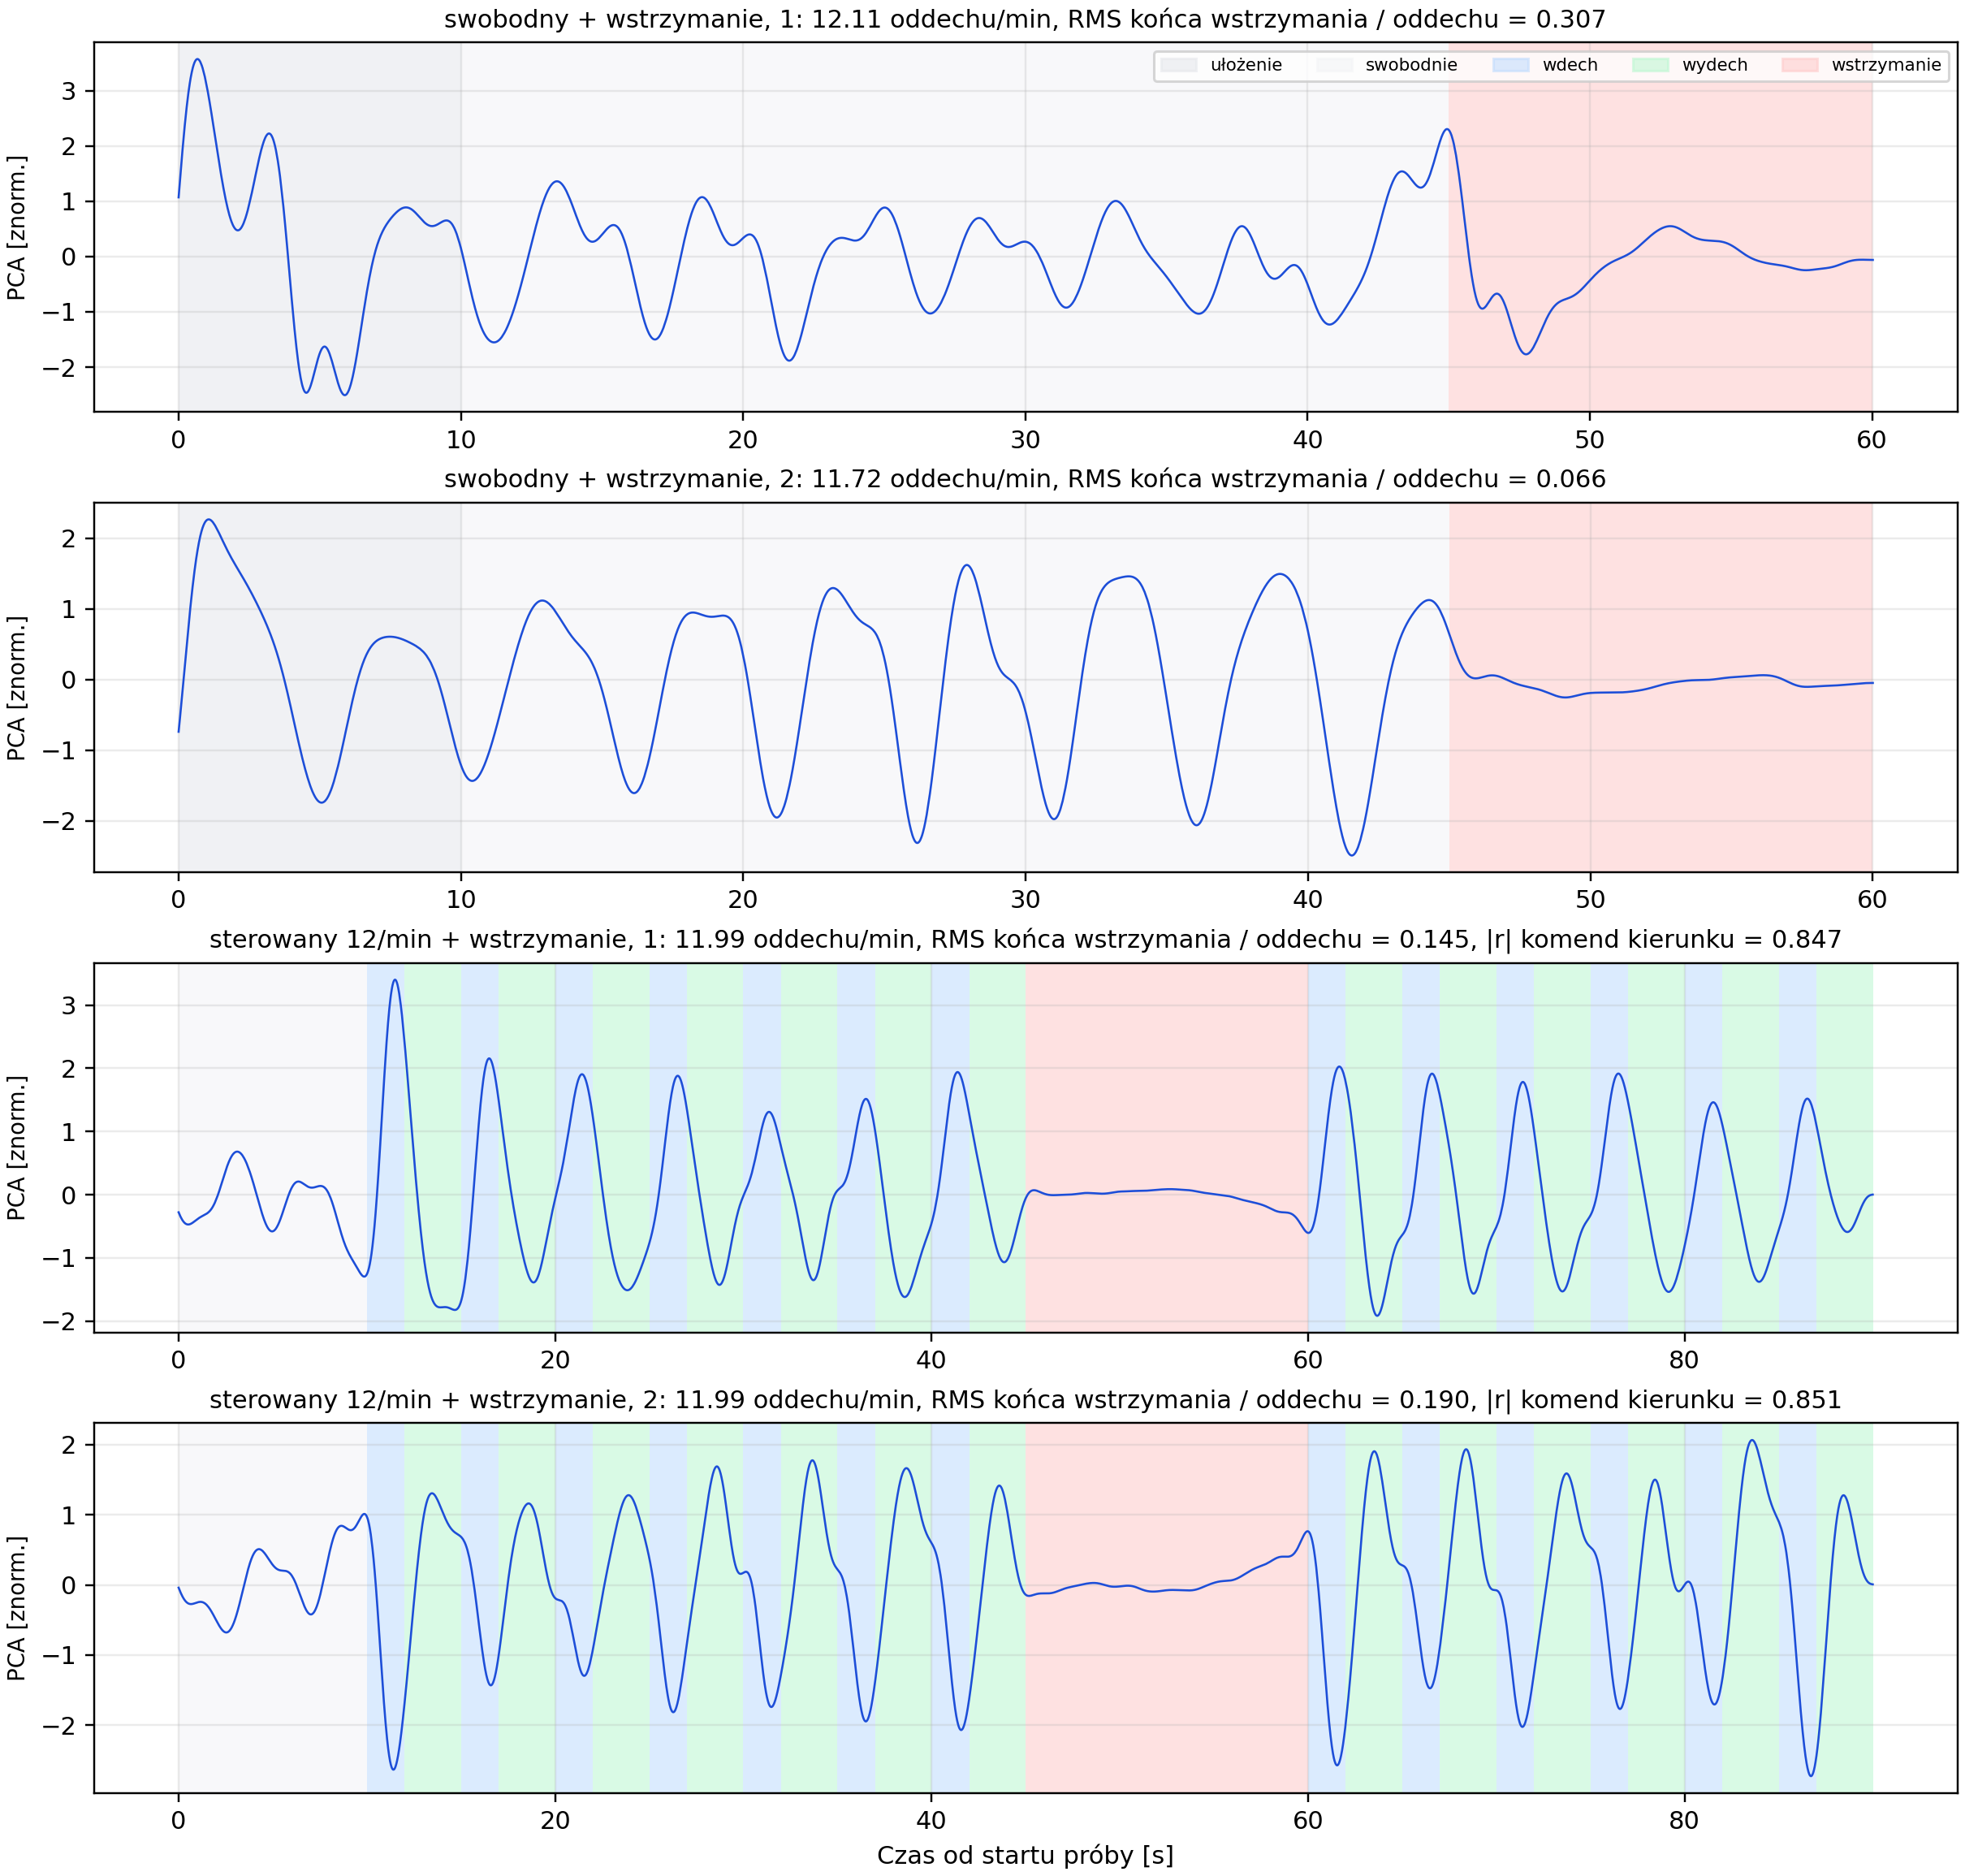
\includegraphics[width=\textwidth]{imu_lsm6ds3_klatka_piersiowa.png}
    \caption[LSM6DS3: cztery próby na klatce piersiowej]{Znormalizowana
    pierwsza składowa główna trzech osi przyspieszenia LSM6DS3 po filtracji
    pasmowej \SIrange{0.07}{0.60}{Hz}. Zacienienie oznacza harmonogram
    komend; znak PCA jest umowny. Dwa dolne przebiegi odtwarzają rytm
    12~oddechów/min, a~we wszystkich czterech próbach końcowa część fazy
    wstrzymania ma wyraźnie mniejszą amplitudę.}
    \label{fig:imu-lsm-klatka}
\end{figure}

\section{Porównanie LSM6DS3 i~iPhone}
\label{sec:imu-iphone-porownanie}

Porównanie wykonano w~dwóch próbach po \SI{90}{s}, wyłącznie w~pozycji na
plecach. Telefon i~moduł LSM6DS3 leżały obok siebie na górnej części klatki
piersiowej, w~tej samej orientacji. Harmonogram każdej próby obejmował
\SI{10}{s} oddechu swobodnego, 7~cykli wdech \SI{2}{s}/wydech \SI{3}{s},
\SI{15}{s} wstrzymania po wydechu i~6~dalszych cykli o~tym samym rytmie.
Telefon pracował z~zadaną częstotliwością \SI{100}{Hz}; zapis obejmuje
zarówno próbki LSM6DS3 z~licznikiem urządzenia, jak i~próbki iPhone
otrzymane przez BLE.

Jakość transmisji obu torów była wystarczająca do porównania. W~dwóch
próbach LSM6DS3 dostarczył odpowiednio 9119 i~9120 próbek przy \SI{100}{Hz},
bez luk licznika, duplikatów, resetów ani niepoprawnych wierszy UART. iPhone
dostarczył po 9012 próbek, czyli ponad 100\% oczekiwanej liczby i~czasu okna
nagrania (niewielki nadmiar wynika z~próbek na jego granicach). Każdy zapis
iPhone obejmował 751 pakietów BLE, bez utraconych, zduplikowanych ani
niepoprawnych pakietów; największa luka pomiędzy kolejnymi próbkami wyniosła
\SI{10}{ms}. W~odróżnieniu od wcześniejszej, niekompletnej transmisji jest to
ciągły strumień obejmujący całe dwa okna pomiarowe.

Tabela~\ref{tab:imu-iphone-wyniki} porównuje cechy wyznaczone tą samą
filtracją pasmową i~PCA trzech osi przyspieszenia. $Q_{\mathrm{spec}}$ jest
stosunkiem najwyższego piku widma do mediany pozostałej części pasma
oddechowego, wyrażonym w~dB; jest zatem wskaźnikiem czytelności piku, a~nie
kalibrowanym SNR toru pomiarowego. $|\rho_{\mathrm{cue}}|$ oznacza
bezwzględną korelację pochodnej PCA z~naprzemiennymi komendami wdechu
i~wydechu po dopasowaniu czasowym. Wartość bezwzględną stosuje się dlatego,
że znak pierwszej składowej głównej zależy od orientacji czujnika.

\begin{table}[H]
\centering
\caption{Porównanie LSM6DS3 i~iPhone w~dwóch próbach sterowanych
\SI{12}{oddech\per\minute}. Wartości w~komórkach zapisano jako
LSM6DS3 / iPhone.}
\label{tab:imu-iphone-wyniki}
\begin{tabular}{@{}lrrr@{}}
\toprule
Próba & $f_R$ [oddech/min] & $Q_{\mathrm{spec}}$ [dB] & $|\rho_{\mathrm{cue}}|$ \\
\midrule
1 & 12,06 / 11,94 & 14,2 / 28,4 & 0,689 / 0,779 \\
2 & 12,07 / 11,99 & 18,9 / 20,8 & 0,739 / 0,760 \\
\bottomrule
\end{tabular}
\end{table}

Oba tory odtworzyły rytm bliski wartości zadanej \SI{12}{oddech\per\minute}.
Różnica między ich estymatami wyniosła odpowiednio 0,12 i~0,08~oddechu/min,
a~iPhone osiągnął w~tych dwóch krótkich seriach wyższy wskaźnik
$Q_{\mathrm{spec}}$. W~końcowych \SI{10}{s} wstrzymania iloraz RMS względem
części oddechowej wyniósł 0,335 i~0,120 dla LSM6DS3 oraz 0,200 i~0,228 dla
iPhone, co w~obu przypadkach potwierdza wyraźne zmniejszenie ruchu.
Rysunek~\ref{fig:imu-iphone-porownanie} pokazuje zgodność odtwarzanego rytmu
z~harmonogramem w~obu urządzeniach. Nie porównuje się jednak bezwzględnej
amplitudy, znaku ani fazy PCA: czujniki mają różne skale, niezależne zegary
i~nie były walidowane względem referencyjnego toru ruchu. Wynik potwierdza
użyteczność obu strumieni do estymacji rytmu w~tej ustalonej geometrii, lecz
nie jest oceną dokładności oddechowej dla innych ułożeń ani pomiarem tętna.

\begin{figure}[H]
    \centering
    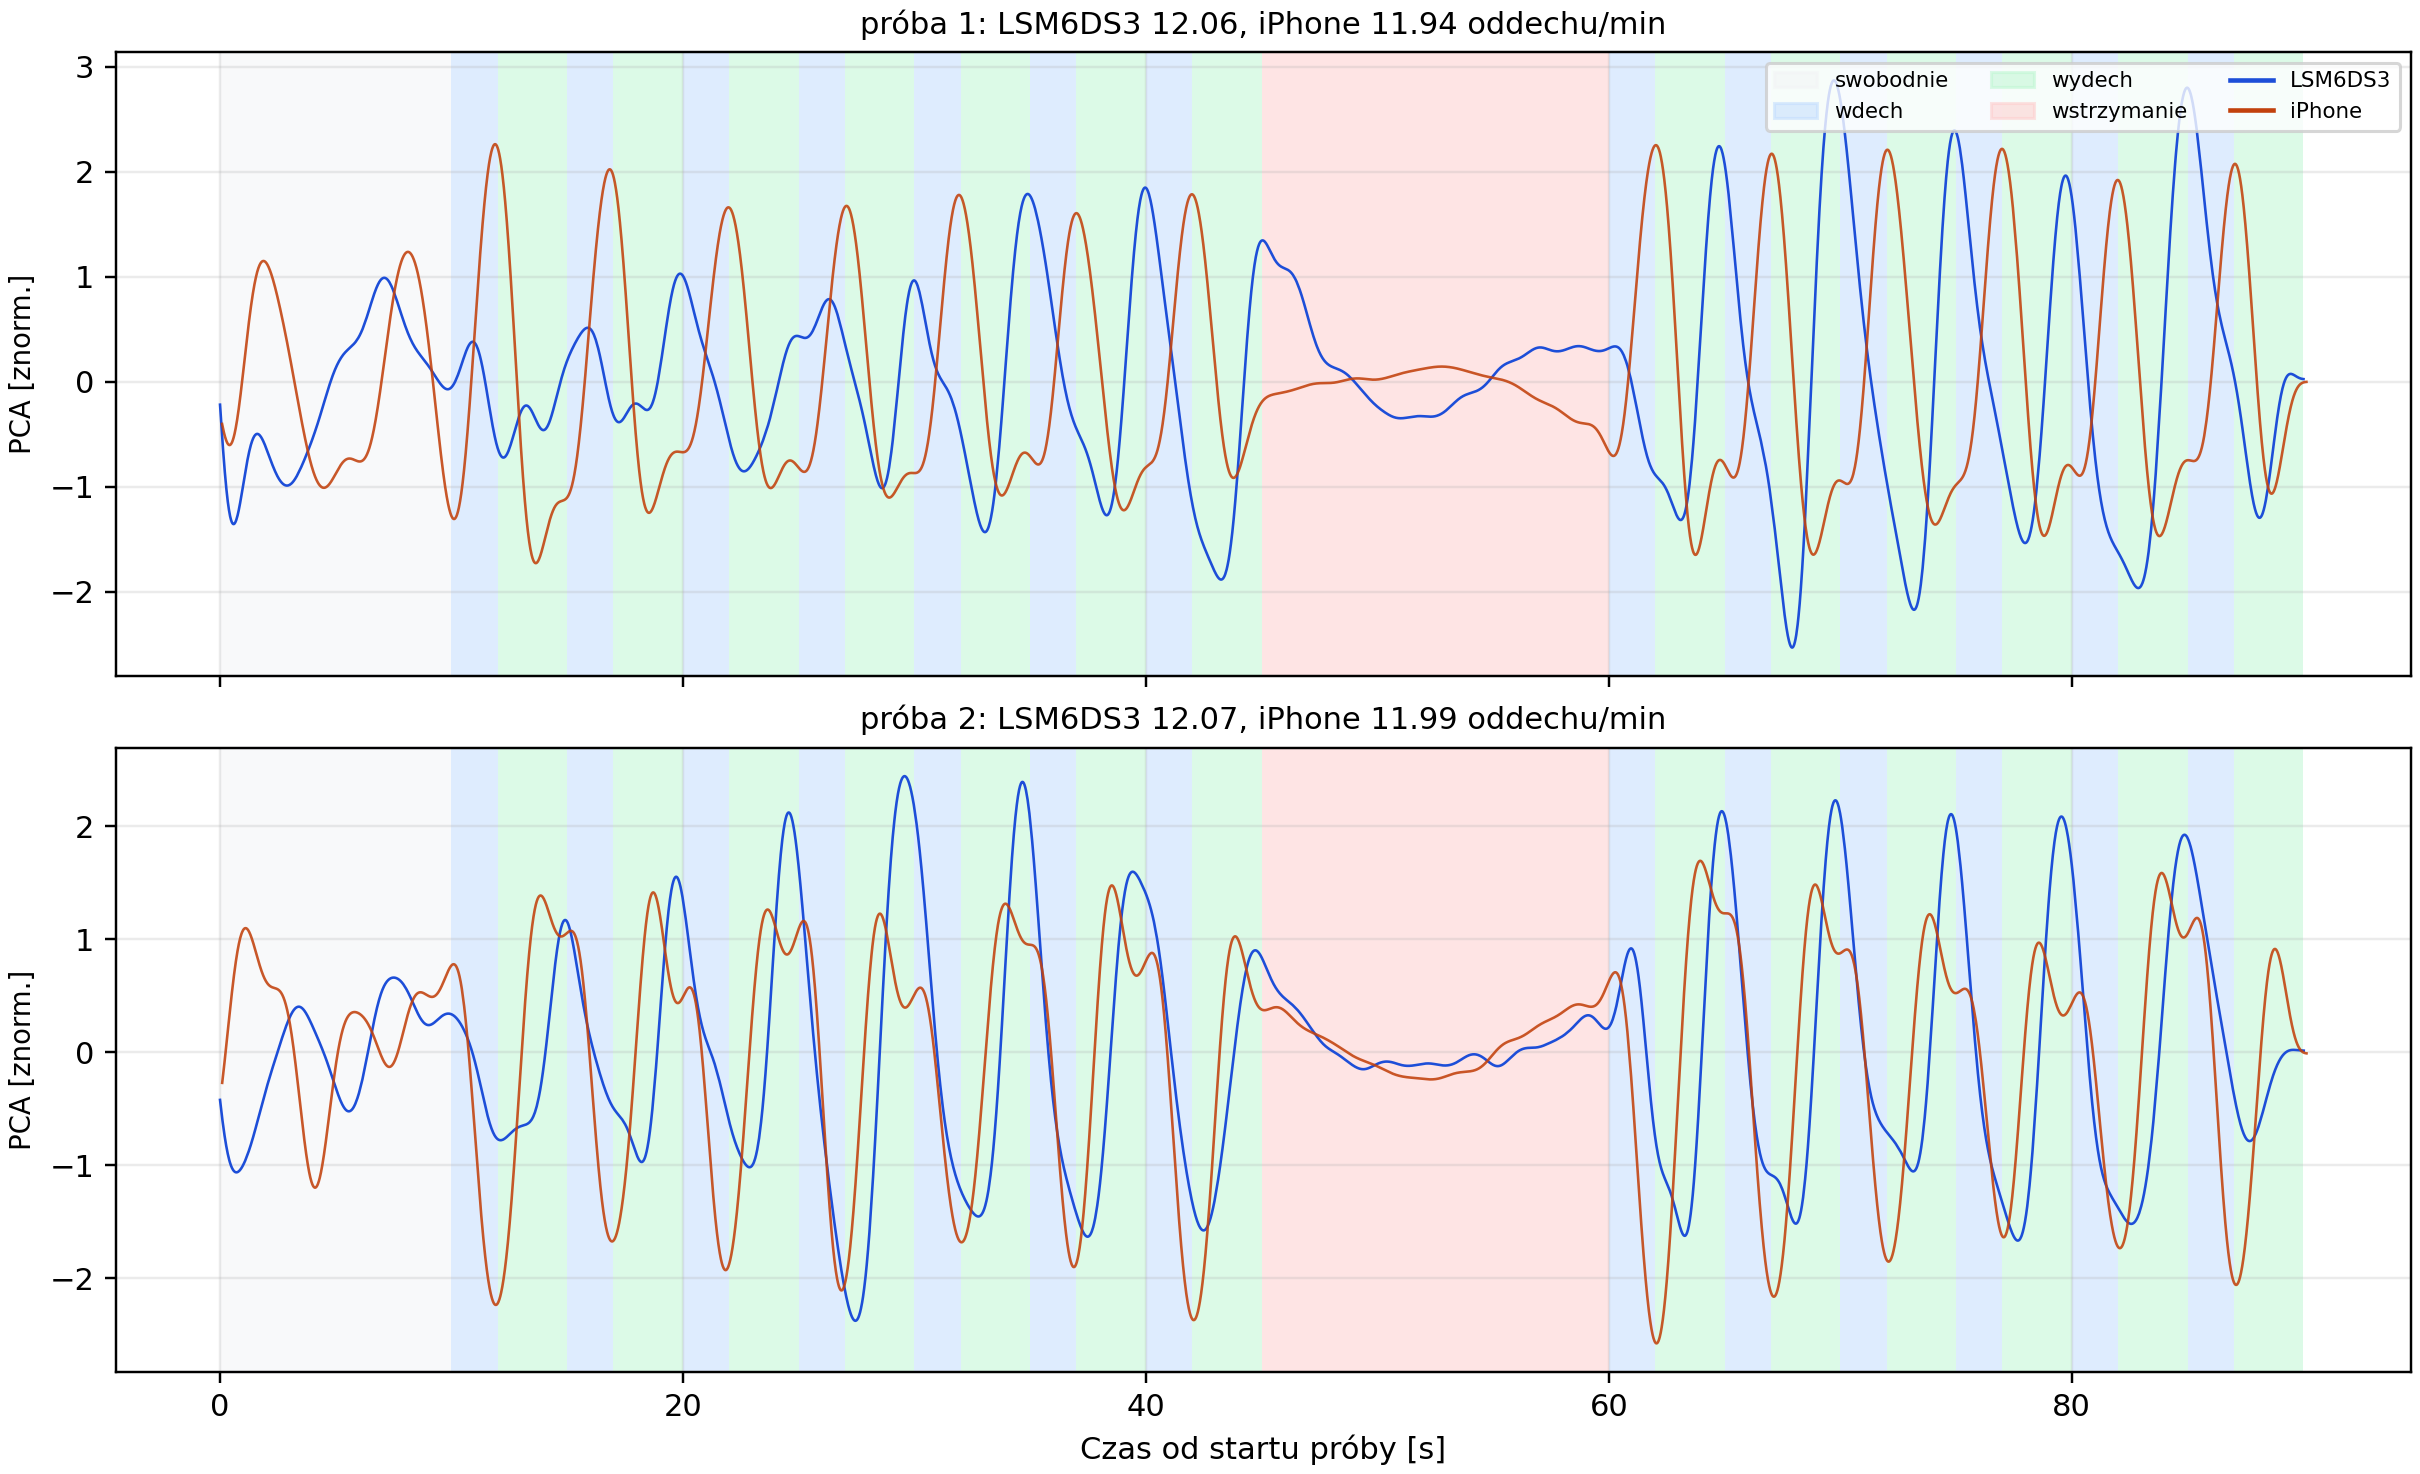
\includegraphics[width=\textwidth]{imu_lsm6ds3_iphone_porownanie.png}
    \caption[Porównanie przebiegów IMU LSM6DS3 i iPhone]{Znormalizowane
    przebiegi PCA przyspieszeń z~LSM6DS3 (niebieski) i~iPhone (pomarańczowy)
    po tej samej filtracji pasmowej \SIrange{0.07}{0.60}{Hz}. Tło oznacza
    kolejne komendy programu prowadzącego. Osie czasu odnoszą się do wspólnego
    czasu hosta; znaku i~bezwzględnej amplitudy PCA nie interpretuje się
    fizycznie.}
    \label{fig:imu-iphone-porownanie}
\end{figure}

\subsection{Poziom resztkowego ruchu w~bezruchu}
\label{sec:imu-spoczynek}

W~tym samym ułożeniu wykonano dodatkowy, \SI{60}{s} zapis bez celowego ruchu.
Jego celem nie była rejestracja oddechu ani tętna, lecz określenie tła
widocznego w~danych udostępnianych przez oba tory: czujnik, firmware albo
aplikację oraz transmisję. Oba strumienie były kompletne: LSM6DS3 dostarczył
6079 próbek przy \SI{100}{Hz}, bez luk licznika, a~iPhone 6000 próbek w~500
pakietach BLE, również bez strat. Maksymalny odstęp między próbkami iPhone
wyniósł \SI{10}{ms}.

Tabela~\ref{tab:imu-spoczynek} zestawia RMS wektora trzech osi po usunięciu
trendu liniowego oraz RMS pierwszej składowej PCA po filtracji w~paśmie
oddechowym i~w~paśmie \SIrange{0.8}{3.0}{Hz}, wykorzystywanym tu wyłącznie
jako pasmo potencjalnej składowej sercowej. Nie jest to próba wykrywania
tętna. W~całym zakresie LSM6DS3 miał niższy poziom resztkowy: około
1,8-krotnie dla surowego wektora przyspieszeń, 1,6-krotnie w~paśmie oddechu
i~1,5-krotnie w~drugim paśmie. Różnica dla żyroskopu jest niewielka.

\begin{table}[H]
\centering
\caption{Porównanie sygnału resztkowego w~\SI{60}{s} bezruchu.}
\label{tab:imu-spoczynek}
\begin{tabular}{@{}lrrrr@{}}
\toprule
Tor & $\sigma_{a}$ [mg] & $\sigma_{\omega}$ [\si{\degree\per\second}] &
$\sigma_{\mathrm{PCA},R}$ [mg] & $\sigma_{\mathrm{PCA},H}$ [mg] \\
\midrule
LSM6DS3 & 0,697 & 0,0728 & 0,0592 & 0,1026 \\
iPhone & 1,246 & 0,0816 & 0,0943 & 0,1591 \\
\bottomrule
\end{tabular}
\end{table}

Rysunek~\ref{fig:imu-spoczynek-widmo} nie pokazuje w~żadnym torze
pojedynczego dominującego piku w~paśmie oddechowym ani w~paśmie potencjalnej
składowej sercowej. Wynik oznacza, że w~tym pojedynczym ułożeniu LSM6DS3 daje
niższe tło niż aplikacja iPhone, nie zaś że jest ogólnie lepszym czujnikiem
oddechu. Na klatce piersiowej iPhone uzyskał wyższy wskaźnik czytelności piku
w~dwóch wcześniejszych próbach, więc o~użyteczności decydują również sposób
mocowania, dynamika ruchu oraz przetwarzanie systemowe.

\begin{figure}[H]
    \centering
    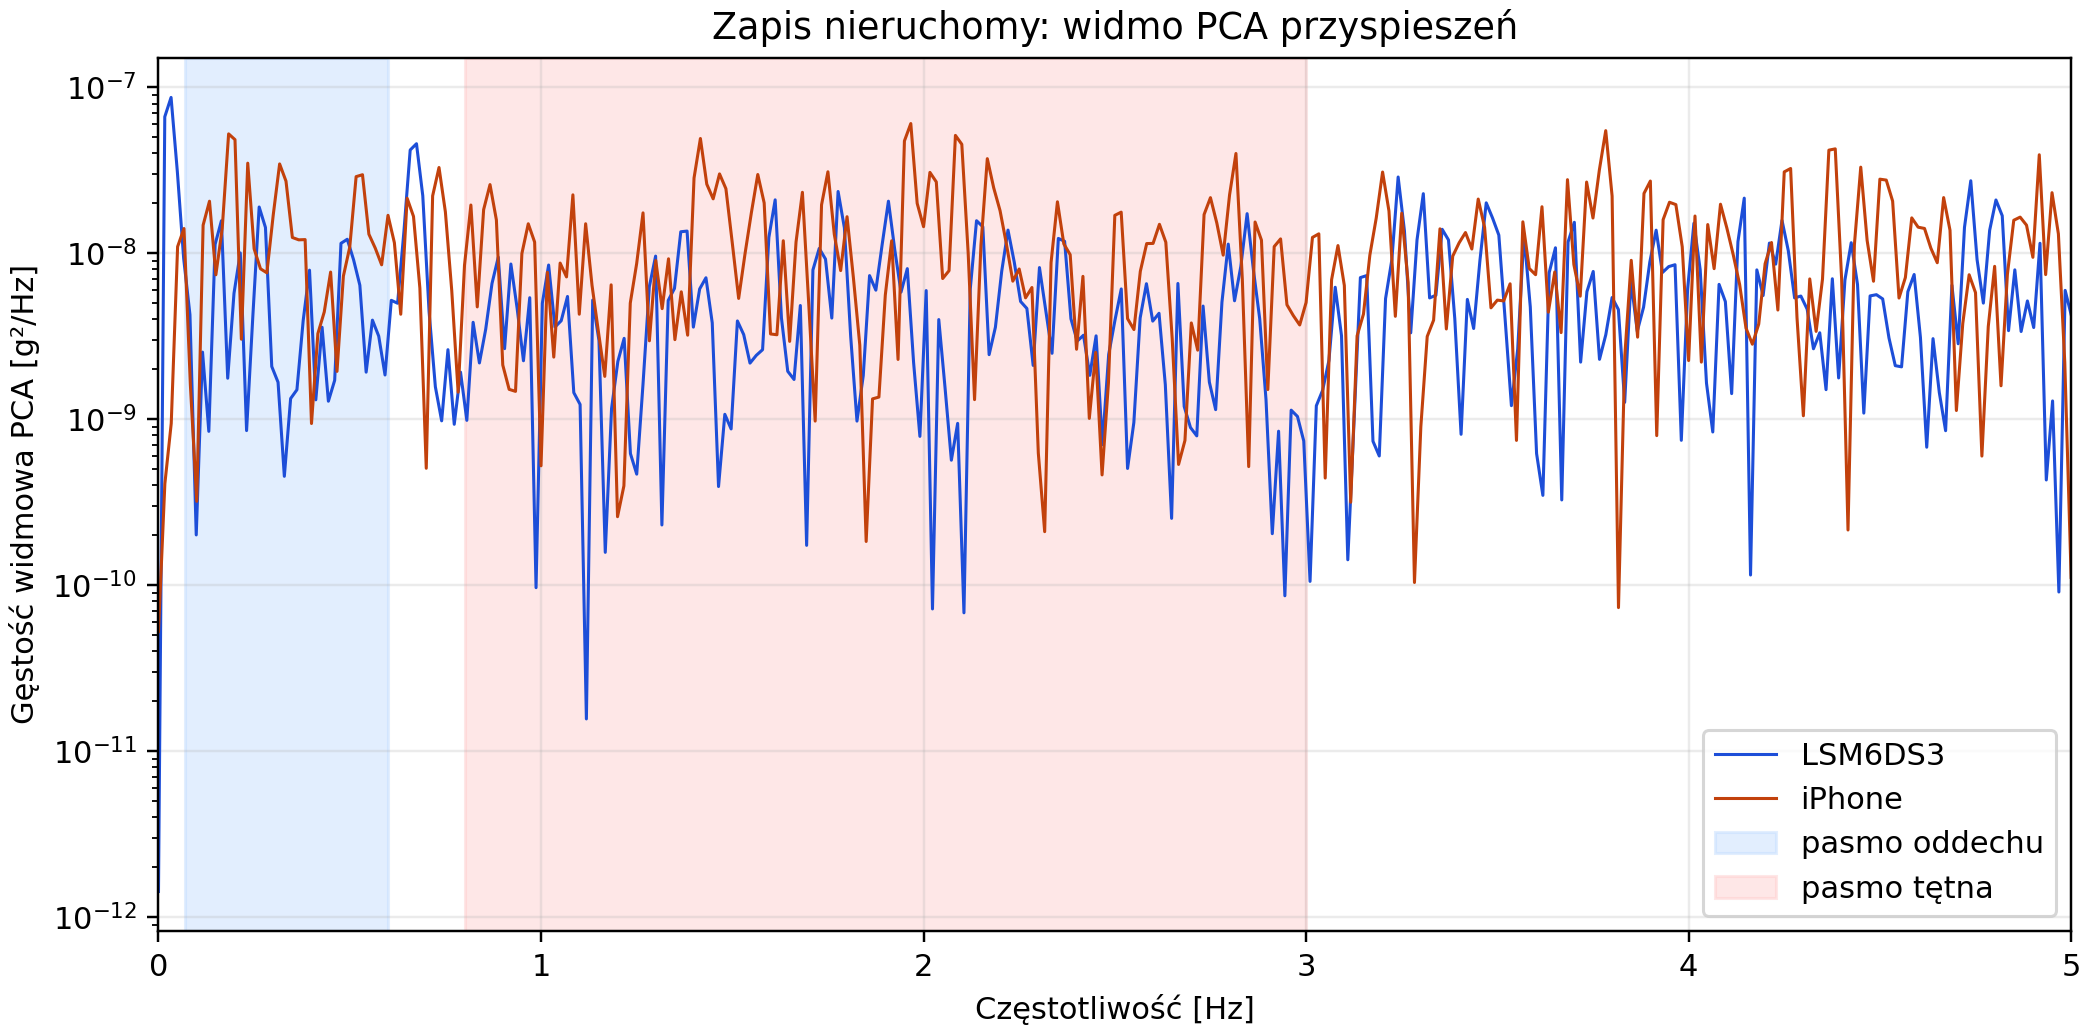
\includegraphics[width=0.92\textwidth]{imu_lsm6ds3_iphone_static_widmo.png}
    \caption[Widmo IMU w bezruchu]{Gęstość widmowa pierwszej składowej PCA
    przyspieszeń podczas \SI{60}{s} bezruchu. Zaznaczono pasmo oddechowe oraz
    pasmo \SIrange{0.8}{3.0}{Hz}; nie jest to wynik detekcji tętna.}
    \label{fig:imu-spoczynek-widmo}
\end{figure}

% ---------------------------------------------------------------------
\chapter{Algorytmy estymacji oddechu i tętna}
\label{chap:algorytmy}

Rozdział ten opisuje najobszerniejszą część własnej pracy programistycznej:
potok przetwarzania, który z~surowych danych Sparse~IQ czujnika A121 wyznacza
częstość oddechu i~tętno. Implementacja liczy około 2300~linii
(\texttt{src/\allowbreak respi\_net/\allowbreak a121\_vitals.py}) i~składa się z~dwóch ścieżek:
\begin{itemize}
  \item \texttt{analyze\_a121\_vitals()} --- bezstanowy analizator okna,
  używany do analizy nagrań CSV i~historii; to on dostarcza wszystkich liczb
  prezentowanych w~tej pracy,
  \item \texttt{A121LiveTraceProcessor} --- stanowy procesor strumieniowy
  z~pamięcią filtrów IIR, używany wyłącznie do rysowania przebiegów na żywo,
  tak aby raz narysowana próbka nie zmieniała już kształtu przy kolejnym
  odświeżeniu wykresu.
\end{itemize}

Świadomie opisano tu również \emph{drogę dojścia} do obecnej postaci
algorytmu. Pierwsza wersja, mimo poprawnej teorii, dawała wyniki bezużyteczne;
sekcja~\ref{sec:co-nie-dzialalo} zestawia kolejne awarie, ich przyczyny
i~zastosowane rozwiązania.

\section{Model sygnału}
\label{sec:model-sygnalu}
Czujnik zwraca dla każdej ramki $n$ i~bramki odległościowej $k$ liczbę
zespoloną
\begin{equation}
  z[n,k] = A[n,k]\,\mathrm{e}^{\,\mathrm{j}\varphi[n,k]},
  \label{eq:iq}
\end{equation}
gdzie amplituda $A$ opisuje siłę odbicia, a~faza $\varphi$ --- drogę optyczną
fali. Fala pokonuje drogę do celu i~z~powrotem, więc dla celu oddalonego
o~$d$ moduł fazy echa wynosi $|\varphi| = 4\pi d/\lambda$, a~zależność
wykorzystywana w~całym potoku ma postać
\begin{equation}
  \Delta d = \frac{\lambda}{4\pi}\,\Delta\varphi .
  \label{eq:faza-przemieszczenie}
\end{equation}
Dla $f_0 = \SI{60}{GHz}$ mamy $\lambda \approx \SI{5}{mm}$, a~więc
$\SI{1}{rad}$ zmiany fazy odpowiada zaledwie \SI{0.4}{mm} przemieszczenia.
To właśnie ta czułość --- a~nie amplituda --- jest źródłem informacji
o~parametrach życiowych.

\paragraph{Konwencja znaku.} Znak w~równaniu~\eqref{eq:faza-przemieszczenie}
nie jest prawem fizycznym, lecz konsekwencją konwencji zespolonej przyjętej
w~czujniku: dla zapisu $\mathrm{e}^{+\mathrm{j}\omega t}$ faza echa maleje
z~odległością, a~dla $\mathrm{e}^{-\mathrm{j}\omega t}$ --- rośnie. Jest to
zatem właściwość toru, stała dla danego czujnika i~danego potoku
przetwarzania, a~nie wielkość losowa zmieniająca się między nagraniami. Dla
A121 i~opisanego tu potoku obowiązuje konwencja $\varphi = +4\pi d/\lambda$:
oddalenie celu zwiększa fazę, a~zbliżenie ją zmniejsza, co czyni
równanie~\eqref{eq:faza-przemieszczenie} poprawnym w~zapisanej postaci.
Konwencję tę ustalono empirycznie i~potwierdzono w~19~niezależnych nagraniach
sterowanych (rozdziały~\ref{chap:hb100-a121-pomiar}
i~\ref{chap:soczewki}): w~każdym z~nich zrekonstruowane przemieszczenie
korelowało \emph{dodatnio} ze wzorcem oddechowym bez jakiejkolwiek korekty
znaku. Wynika z~niej bezpośrednio kierunek fazy cyklu wykorzystywany
w~sekcji~\ref{sec:etapy-przetwarzania-oddechu}: wdech zbliża klatkę do radaru,
więc $d$ maleje, faza maleje, a~przebieg wyjściowy \emph{opada}.

Skala zjawisk, które trzeba rozdzielić, jest jednak skrajnie nierówna:
ruch klatki piersiowej przy spokojnym oddechu wynosi \SIrange{4}{12}{mm},
natomiast mikroruch powierzchni ciała wywołany pracą serca to zaledwie
\SIrange{0.2}{0.5}{mm}. Sygnał sercowy jest więc o~\emph{rząd do dwóch rzędów
wielkości słabszy} od oddechowego i~w~dodatku leży w~paśmie, w~które wpadają
harmoniczne oddechu. Cała trudność algorytmu tętna sprowadza się do tego
jednego faktu i~to jemu poświęcona jest sekcja~\ref{sec:tetno}.

\begin{figure}[H]
    \centering
    \begin{tikzpicture}[node distance=5.5mm and 7mm]
      \node[wejscie] (iq)    {Sparse IQ\\$z[n,k]$};
      \node[blok, right=of iq] (fs) {estymacja $f_s$\\(korekcja burstów)};
      \node[blok, right=of fs] (clut) {usunięcie\\echa statycznego};
      \node[blok, right=of clut] (gate) {wybór bramek\\i~wagi};

      \node[blok, below=9mm of gate] (faza) {faza różnicowa\\(centrowanie IQ)};
      \node[blok, left=of faza] (oddech) {pasmo oddechu\\\SIrange{0.10}{0.50}{Hz}};
      \node[blok, left=of oddech] (serce) {usunięcie ruchu\\skorelowanego};
      \node[blok, left=of serce] (pasmoh) {pasmo serca\\\SIrange{0.70}{2.00}{Hz}};

      \node[wynik, below=9mm of oddech] (rr) {częstość oddechu\\$f_r$ [odd./min]};
      \node[blok, below=9mm of pasmoh] (kand) {kandydaci widmowi\\+ walidator czasowy};
      \node[wynik, below=9mm of kand] (hr) {tętno\\$f_h$ [ud./min]};

      \draw[strzalka] (iq) -- (fs);
      \draw[strzalka] (fs) -- (clut);
      \draw[strzalka] (clut) -- (gate);
      \draw[strzalka] (gate) -- (faza);
      \draw[strzalka] (faza) -- (oddech);
      \draw[strzalka] (oddech) -- (serce);
      \draw[strzalka] (serce) -- (pasmoh);
      \draw[strzalka] (oddech) -- (rr);
      \draw[strzalka] (pasmoh) -- (kand);
      \draw[strzalka] (kand) -- (hr);
      \draw[strzalka] (rr.west) -| node[font=\scriptsize, pos=0.78, right=1pt]
        {$f_r$} (serce.south);
    \end{tikzpicture}
    \caption[Schemat potoku przetwarzania sygnału A121]{Potok przetwarzania
    sygnału A121. Ścieżka oddechowa jest krótka i~stabilna; ścieżka sercowa
    wymaga dodatkowo usunięcia ruchu skorelowanego z~oddechem oraz walidacji
    kandydatów w~dziedzinie czasu. Estymowana częstość oddechu $f_r$ wraca
    jako parametr do toru sercowego.}
    \label{fig:potok}
\end{figure}

\section{Estymacja częstotliwości próbkowania}
Pozornie trywialny krok okazał się pierwszym źródłem poważnych błędów.
Ramki są dostarczane przez UART \emph{paczkami}: kilka ramek trafia do hosta
niemal jednocześnie (odstępy poniżej milisekundy, czasem zerowe), po czym
następuje dłuższa przerwa. Naiwny estymator oparty na medianie odstępów
$\hat{f_s} = 1/\mathrm{med}(\Delta t)$ mierzy wtedy odstęp \emph{wewnątrz
paczki}, a~nie rzeczywisty odstęp ramek, i~zawyża $f_s$ nawet kilkukrotnie.
Ponieważ pasma filtrów są definiowane względem $f_s$, całe pasmo oddechowe
przesuwało się poza rzeczywisty rytm i~estymaty były bezwartościowe.

Zaimplementowany estymator (\texttt{sample\_rate\_from\_ms}) wykrywa taką
sytuację i~przełącza się na estymator globalny:
\begin{equation}
  \hat{f_s} =
  \begin{cases}
    \dfrac{N-1}{t_{N-1} - t_0}, & \text{gdy sygnatury czasowe są ,,paczkowe'',}\\[2ex]
    \left(\overline{\Delta t}\,\right)^{-1}, & \text{w~przeciwnym razie,}
  \end{cases}
  \label{eq:fs}
\end{equation}
gdzie średnia $\overline{\Delta t}$ jest liczona odpornie, tylko po odstępach
z~przedziału $(0{,}25\,\mathrm{med},\ 4\,\mathrm{med})$. Za ,,paczkowe'' uznaje
się sygnatury, w~których ponad 5\% odstępów jest niedodatnich lub krótszych
niż $\max(\SI{2}{ms},\ 0{,}2\,\mathrm{med})$, albo w~których obie estymaty
różnią się o~więcej niż 25\%.

\section{Usunięcie echa statycznego i~wybór bramki odległościowej}
\label{sec:bramkowanie}
Dominującą składową sygnału nie jest człowiek, lecz nieruchome otoczenie
(ściana, rama łóżka, sam korpus czujnika). Odbicia te są stałe w~czasie,
więc usuwa się je filtrem górnoprzepustowym w~dziedzinie ramek:
\begin{equation}
  z_m[n,k] = z[n,k] - \mathrm{LP}\big(z[\cdot,k]\big)[n],
  \label{eq:clutter}
\end{equation}
gdzie $\mathrm{LP}$ jest filtrem Butterwortha dolnoprzepustowym o~częstotliwości
granicznej równej dolnej granicy pasma oddechowego (\SI{0.10}{Hz}). Sygnał
$z_m$ służy do \emph{oceny amplitudy} bramek --- ale, co kluczowe,
\textbf{nie do wyznaczania fazy} (patrz sekcja~\ref{sec:faza}).

Każdą bramkę ocenia się dwoma niezależnymi kryteriami. Pierwszym jest
medianowa amplituda po usunięciu echa, $\mathrm{med}_n |z_m[n,k]|$. Drugim ---
stosunek energii w~paśmie życiowym do energii tła:
\begin{equation}
  R_k = \frac{\big\langle |\Phi_k(f)|^2 \big\rangle_{f \in [0{,}10;\,2{,}00]\,\mathrm{Hz}}}
             {\big\langle |\Phi_k(f)|^2 \big\rangle_{f \in [0{,}03;\,5]\,\mathrm{Hz}\setminus\text{pasmo życiowe}}},
  \label{eq:ber}
\end{equation}
gdzie $\Phi_k$ jest widmem fazy $k$-tej bramki. Bramka z~silnym odbiciem, ale
bez periodycznej modulacji (np. metalowa rama łóżka), ma wysoką amplitudę
i~niskie $R_k$ --- i~zostaje odrzucona. Sama amplituda nie wystarcza.

Cel wybiera się jako bramkę o~najwyższym łącznym wyniku, a~następnie tworzy
wokół niej klaster bramek w~promieniu bramkowania. Sygnał wypadkowy jest
średnią ważoną amplitudą, przy czym do estymacji oddechu używa się co najwyżej
3~bramek (torsu nie trzeba szerzej obejmować, a~każda dodatkowa bramka wnosi
szum).

\section{Ekstrakcja fazy: dlaczego nie wprost \texorpdfstring{$\arg z$}{arg z}}
\label{sec:faza}
Naturalny pomysł --- rozwinąć fazę residuum $\arg(z_m)$ i~przefiltrować ---
w~praktyce nie działa i~był jedną z~najkosztowniejszych pomyłek w~projekcie.
Wektor $z_m$ po usunięciu echa statycznego jest \emph{mały} i~przy typowym,
podmilimetrowym ruchu klatki piersiowej regularnie \emph{przechodzi przez
początek układu współrzędnych}. Funkcja $\operatorname{atan2}$ wykonuje wtedy
skok o~$\pi$, którego rozwijanie fazy nie potrafi odróżnić od prawdziwego
ruchu. W~efekcie przebieg po filtracji pasmowej zawierał losowe skoki
i~płaskie odcinki.

Rozwiązanie składa się z~dwóch elementów. Po pierwsze, faza jest wyznaczana
z~\emph{surowego} sygnału $z$ (którego moduł jest duży i~który nie zbliża się
do zera), a~echo statyczne usuwa się dopiero \emph{w~dziedzinie fazy} przez
centrowanie okręgu IQ. Trajektoria $z[n,k]$ dla nieruchomego tła z~drgającym
celem jest łukiem okręgu o~środku $c$ przesuniętym od zera; środek ten
wyznacza się algebraicznym dopasowaniem okręgu (metoda Kåsy), minimalizując
\begin{equation}
  \sum_n \Big( |z[n,k] - c|^2 - r^2 \Big)^2,
  \label{eq:okrag}
\end{equation}
co po podstawieniu $c = (c_x, c_y)$ sprowadza się do liniowego zadania
najmniejszych kwadratów. Dopasowanie przyjmuje się tylko wtedy, gdy jest
wiarygodne (względny błąd promienia poniżej 0,45); w~przeciwnym razie bramka
zachowuje fazę surową.

Po drugie --- i~to jest właściwe zabezpieczenie --- fazę akumuluje się
\emph{przyrostowo}, z~różnic międzyramkowych, zamiast rozwijać fazę
bezwzględną:
\begin{equation}
  \Delta\varphi[n,k] = \arg\!\big( \hat{z}[n,k]\,\hat{z}^{*}[n-1,k] \big),
  \qquad
  \varphi[n,k] = \sum_{i=1}^{n} \Delta\varphi[i,k],
  \label{eq:faza-roznicowa}
\end{equation}
gdzie $\hat{z} = z/|z|$. Kolejne próbki dzieli krótki łuk, więc
$\Delta\varphi$ nigdy nie zbliża się do $\pm\pi$ i~problem niejednoznaczności
znika. Jest to zarazem podejście stosowane w~referencyjnym procesorze
oddechowym firmy Acconeer.

Łączenie bramek wykonuje się \emph{koherentnie}, przed operacją arcus tangens:
\begin{equation}
  \Delta\varphi[n] = \arg \left( \sum_k w_k\, \hat{z}[n,k]\,\hat{z}^{*}[n-1,k] \right),
  \label{eq:koherentne}
\end{equation}
dzięki czemu bramka o~małej wadze wnosi mało energii do sumy, a~nie --- jak
przy uśrednianiu już policzonych faz --- pełnoprawny, zaszumiony kąt.

\section{Estymacja częstości oddechu}
Ścieżka oddechowa jest stosunkowo prosta, ponieważ sygnał jest silny.
Sygnał fazowy jest filtrowany pasmowo w~zakresie
\SIrange{0.10}{0.50}{Hz} (6--30~oddechów/min) filtrem Butterwortha
2.~rzędu w~implementacji zerofazowej (\texttt{sosfiltfilt}, filtracja
w~przód i~w~tył --- brak przesunięcia fazowego kosztem pracy wsadowej),
a~częstość wyznaczana jest z~położenia maksimum gęstości widmowej mocy
w~oknie \SI{20}{s}, z~interpolacją paraboliczną wokół prążka maksymalnego.

Po serii nieudanych prób własnej implementacji ostatecznie zdecydowano się
oprzeć estymację częstości oddechu na \textbf{referencyjnym procesorze
producenta} (\texttt{Breathing\allowbreak Processor} z~pakietu \emph{Acconeer Exploration
Tool}), któremu podaje się wybrany wcześniej segment bramek. Procesor ten
realizuje własne usuwanie echa statycznego (filtr IIR), rozwijanie fazy,
filtrację pasmową, okno Hamminga, uzupełnianie zerami i~interpolację
kwadratową piku. Własna implementacja pozostała jako ścieżka zapasowa na
wypadek zmian w~API biblioteki. Decyzja ta była jednym z~przełomowych momentów
projektu (commit \texttt{9d2130a}, \emph{,,vital signals fix''}).

Pewność estymaty definiowana jest jako wyrazistość piku względem tła w~paśmie:
\begin{equation}
  C_r = \frac{P(f_r)}{\mathrm{med}_{f \in \text{pasmo}} P(f)}.
  \label{eq:conf-resp}
\end{equation}

Dodatkowo zaimplementowano \textbf{detekcję braku oddechu}: jeżeli wartość
skuteczna sygnału oddechowego spada poniżej \SI{0.005}{rad} (próg dobrany
empirycznie dla A121, co odpowiada ruchowi rzędu pojedynczych mikrometrów),
oddech jest nieodróżnialny od szumu czujnika i~zamiast losowej częstotliwości
raportowany jest brak wyniku. Bez tego zabezpieczenia system podczas wstrzymania
oddechu pokazywał ,,oddech'' wzięty z~szumu.

\subsection{Od surowego IQ do przebiegu oddechowego}
\label{sec:etapy-przetwarzania-oddechu}
Sam wynik częstości nie pokazuje, które własności sygnału usuwają kolejne
operacje potoku. Dlatego na rysunku~\ref{fig:a121-oddech-etapy} pokazano ten
sam, stabilny \SI{15}{s} fragment rzeczywistego nagrania A121 po kolejnych
przekształceniach. Najpierw widoczne są nieprzetworzone składowe $I$ i~$Q$.
Moduł residuum po usunięciu echa statycznego służy wyłącznie do wyboru bramki,
nie do wyznaczenia fazy: właśnie dlatego następne panele wracają do surowego
sygnału zespolonego. Faza po wycentrowaniu okręgu IQ, faza różnicowa oraz
koherentne połączenie trzech bramek prowadzą do ostatniego panelu ---
przebiegu po filtrze \SIrange{0.10}{0.50}{Hz}. Różne skale pionowe są celowe:
rysunek obrazuje zmianę postaci sygnału, a~nie zmianę jego bezwzględnej
amplitudy.

\begin{figure}[H]
    \centering
    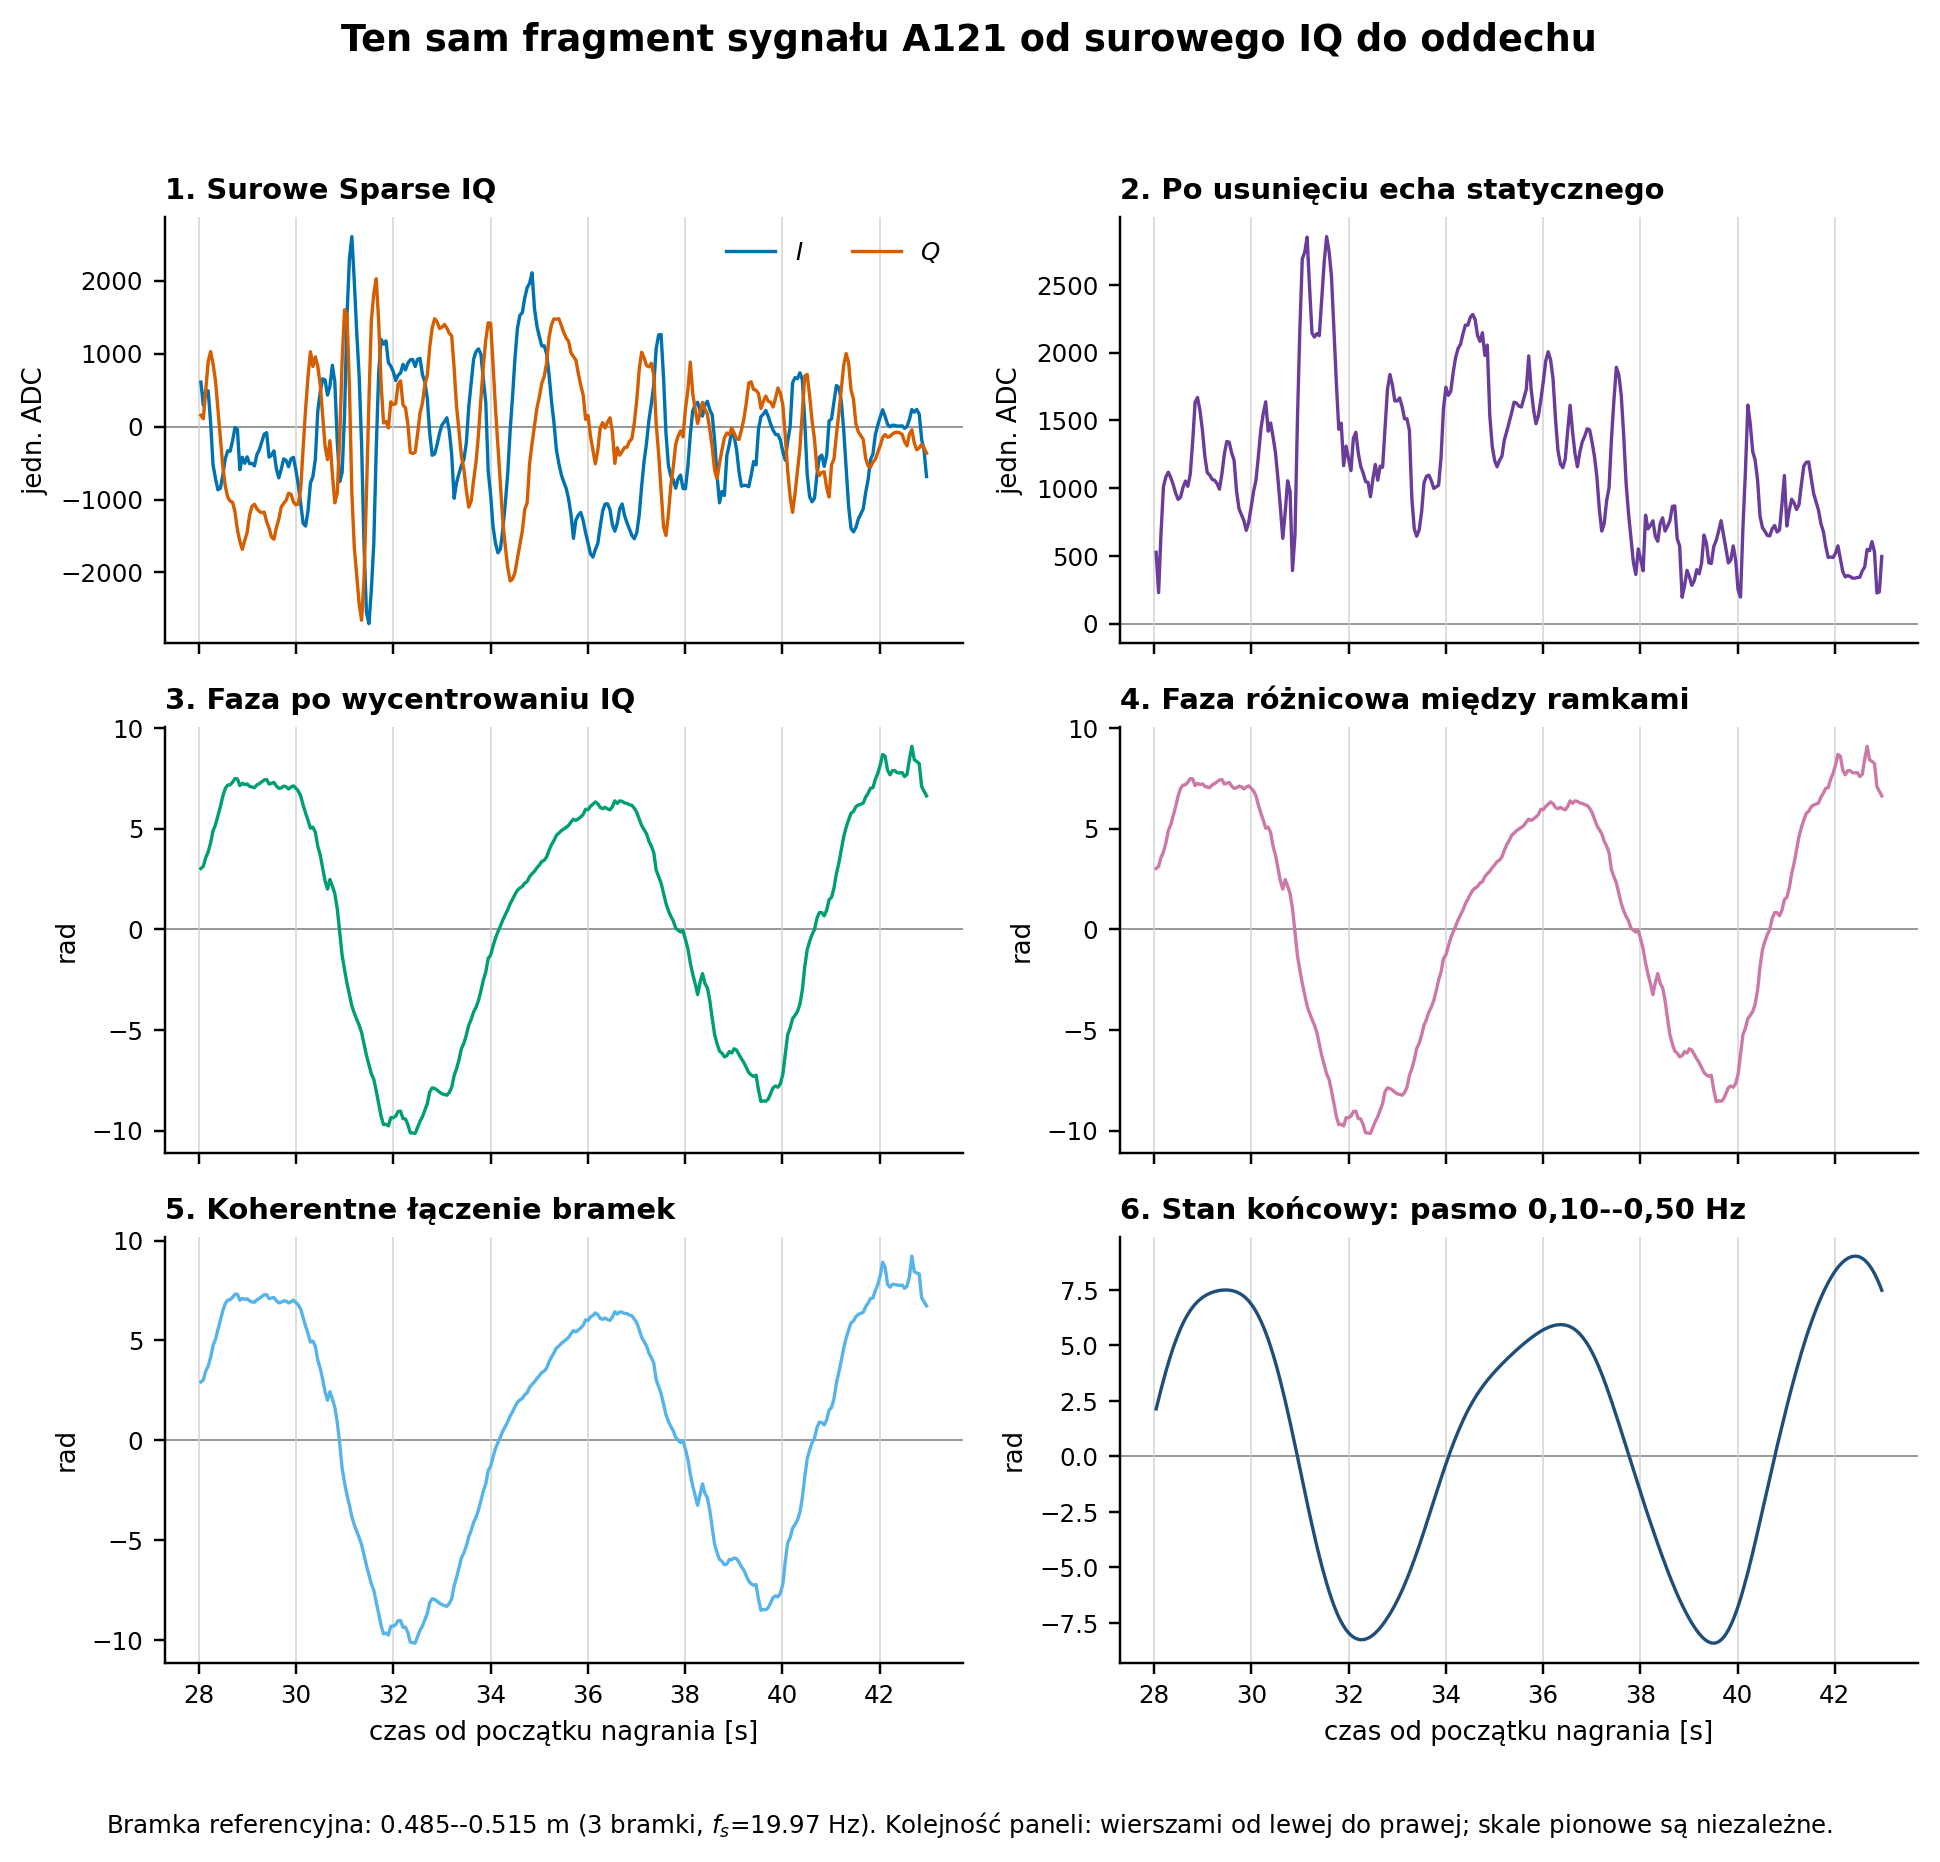
\includegraphics[width=\textwidth]{a121_oddech_etapy_przetwarzania.png}
    \caption[Etapy rekonstrukcji sygnału oddechowego A121]{Kolejne etapy
    rekonstrukcji sygnału oddechowego z~tego samego fragmentu Sparse IQ.
    Panele należy czytać wierszami od lewej do prawej: surowe $I/Q$,
    usunięcie echa statycznego dla wyboru bramki, wycentrowanie IQ, faza
    różnicowa, koherentne łączenie bramek i~końcowa filtracja pasmowa.
    Zastosowano zakres \SIrange{0.485}{0.515}{m}; jest to wynik przetworzenia
    rzeczywistego nagrania, a~nie przebieg syntetyczny.}
    \label{fig:a121-oddech-etapy}
\end{figure}

\paragraph{Deterministyczne znaczniki wdechu i~wydechu.}
Na przefiltrowanym przebiegu można utworzyć prostą, odtwarzalną anotację
wstępną bez modelu uczonego. Detektor szuka maksimów i~minimów po
normalizacji: minimalna prominencja wynosi $0{,}30\,\sigma$, a~minimalny
odstęp między ekstremami jest równy $0{,}45$ okresu wyznaczonego z~maksimum
FFT. Kierunek faz nie jest przy tym dowolnym wyborem, lecz wynika
z~konwencji znaku ustalonej w~sekcji~\ref{sec:model-sygnalu}: wdech zbliża
klatkę do radaru i~zmniejsza fazę, więc przejście od maksimum do minimum
oznacza wdech, a~od minimum do następnego maksimum --- wydech. Nie wykonano ręcznych
poprawek znaczników (rysunek~\ref{fig:a121-oddech-fazy}). Są to zatem
deterministyczne etykiety bazowe przydatne do kontroli danych i~wstępnej
anotacji, lecz nie zastępują referencyjnego pomiaru fizjologicznego ani
weryfikacji ręcznej.

\begin{figure}[H]
    \centering
    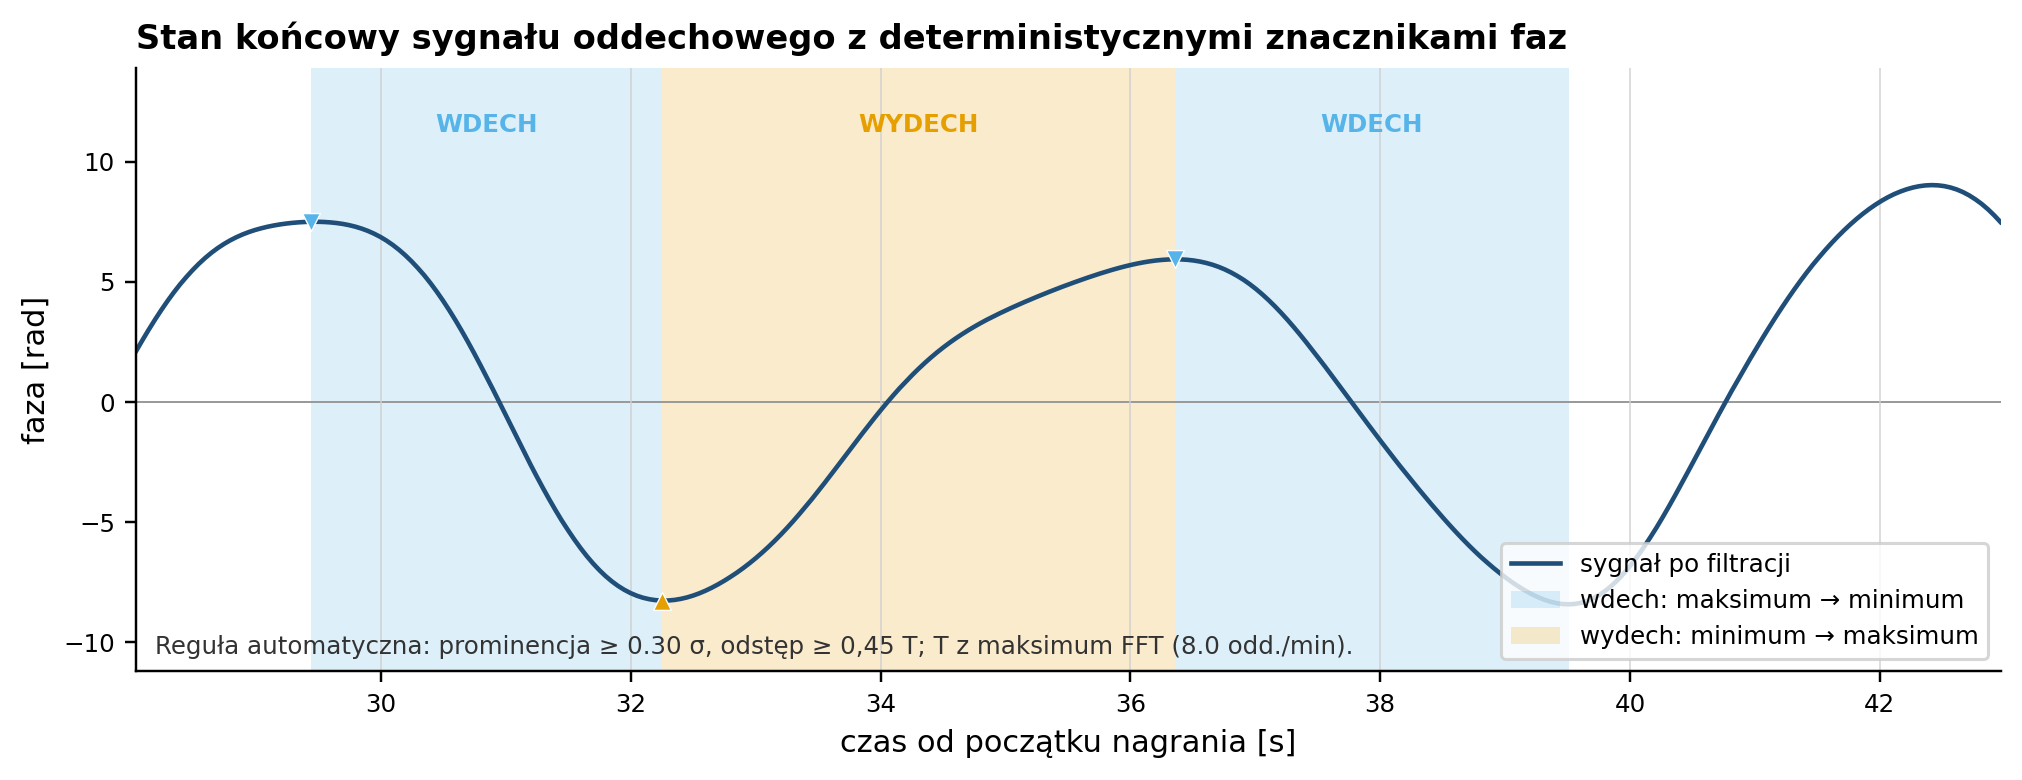
\includegraphics[width=\textwidth]{a121_oddech_fazy_deterministyczne.png}
    \caption[Deterministyczne znaczniki faz oddechu]{Końcowy sygnał oddechowy
    z~nałożonymi znacznikami wyznaczonymi tylko przez ustaloną regułę
    ekstremów. Niebieskie pola oznaczają wdech (maksimum do minimum),
    pomarańczowe --- wydech (minimum do maksimum); trójkąty wskazują początki
    odpowiednich faz.}
    \label{fig:a121-oddech-fazy}
\end{figure}

\section{Estymacja tętna --- problem harmonicznych}
\label{sec:tetno}
Ruch klatki piersiowej przy oddychaniu nie jest sinusoidalny: wdech i~wydech
mają różne profile, przez co widmo oddechu zawiera silne harmoniczne
$n f_r$. Dla typowej częstości spoczynkowej $f_r \approx \SI{0.15}{Hz}$
harmoniczne pojawiają się co \SI{0.15}{Hz}, a~więc \emph{w~całym paśmie
sercowym} \SIrange{0.70}{2.00}{Hz} leży ich kilkanaście (rzędy 5--13).
Ponieważ sygnał sercowy jest 20--50~razy słabszy od oddechowego, harmoniczna
oddechu bywa w~paśmie serca silniejsza niż samo tętno. Prosty detektor
maksimum widma wskazuje wtedy harmoniczną --- i~dokładnie to robiła pierwsza
wersja algorytmu.

Ostateczne rozwiązanie jest kaskadą pięciu mechanizmów; żaden z~nich osobno
nie wystarcza.

\paragraph{1. Usunięcie ruchu skorelowanego z~oddechem.}
Zamiast ,,wycinać'' każdą harmoniczną (co niszczy tętno leżące przypadkiem
w~pobliżu), modeluje się nieliniowość oddechu bezpośrednio. Znormalizowany
przebieg oddechowy $r[n]$ podnosi się do potęg $p = 2,\dots,6$, każdą potęgę
filtruje pasmowo do pasma serca i~traktuje jako regresor. Współczynniki
wyznacza regresja grzbietowa:
\begin{equation}
  \hat{\boldsymbol\beta} = \big(\mathbf{X}^{\!\top}\mathbf{X} + \gamma \mathbf{I}\big)^{-1}
  \mathbf{X}^{\!\top} \mathbf{x},
  \qquad
  \mathbf{X}_{:,p} = \mathrm{BP}_{\text{serce}}\big(r^{\,p}\big),
  \label{eq:regresja}
\end{equation}
a~od sygnału odejmuje się dopasowany artefakt \emph{miękko}, ze współczynnikiem
0{,}70:
\begin{equation}
  x_{\text{serce}}[n] = x[n] - 0{,}70 \cdot \big(\mathbf{X}\hat{\boldsymbol\beta}\big)[n].
  \label{eq:miekkie-odejmowanie}
\end{equation}
Niepełne odejmowanie jest celowe: dzięki niemu prawdziwe tętno leżące blisko
harmonicznej przetrwa i~może zostać odzyskane przez walidator z~punktu~4.

\paragraph{2. Filtracja pasmowa i~kandydaci widmowi.}
Sygnał filtruje się pasmowo (\SIrange{0.70}{2.00}{Hz}, Butterworth 3.~rzędu,
zerofazowo), a~z~widma mocy wybiera się nie jedno maksimum, lecz do sześciu
kandydatów. Widmo jest przed wyborem modyfikowane wycięciami gaussowskimi
w~miejscach harmonicznych oddechu:
\begin{equation}
  S(f) = P(f) \prod_{n=2}^{7}
  \left[ 1 - 0{,}75 \exp\!\left( -\tfrac{1}{2}\Big(\tfrac{f - n f_r}{\sigma_n}\Big)^{\!2} \right) \right],
  \qquad \sigma_n = \max(0{,}040,\ 0{,}030\, n f_r).
  \label{eq:notch}
\end{equation}
Pierwotne wycięcia były wąskie i~płytkie, przez co przepuszczały większość
energii harmonicznej; obecne są szersze i~tłumią o~\SI{-12}{dB}.

\paragraph{3. Tłumienie prążków brzegowych.}
Energia zbocza filtra gromadzi się w~skrajnych prążkach FFT, przez co detektor
regularnie ,,zatrzaskiwał się'' na dokładnie \SI{0.70}{Hz} (42~ud./min ---
podejrzanie równa dolna granica pasma). Na obu krańcach pasma nałożono
liniowe okno tłumiące o~szerokości około \SI{0.05}{Hz}.

\paragraph{4. Walidacja w~dziedzinie czasu.}
Kluczowa obserwacja: harmoniczna oddechu jest silna \emph{widmowo}, ale rzadko
tworzy regularny ciąg uderzeń w~czasie. Każdego kandydata $f$ weryfikuje się
więc, zawężając sygnał wokół $f$ i~szukając w~nim ciągu pików. Ocena
periodyczności łączy cztery składniki:
\begin{equation}
  s(f) = 0{,}38\,g + 0{,}27\,\rho + 0{,}20\,c + 0{,}15\,\sigma_{\text{span}},
  \label{eq:periodycznosc}
\end{equation}
gdzie $g$ to frakcja odstępów międzypikowych mieszczących się w~$\pm32\%$
oczekiwanego okresu $1/f$, $\rho = \max(0,\ 1 - \mathrm{CV}/0{,}42)$ jest miarą
regularności opartą na współczynniku zmienności odstępów, $c$ --- pokryciem
(stosunek liczby znalezionych pików do oczekiwanej), a~$\sigma_{\text{span}}$
--- częścią okna faktycznie objętą ciągiem pików.

Wynik końcowy łączy pewność widmową i~periodyczność, przy czym kandydat
leżący na harmonicznej i~jednocześnie słabo periodyczny ($s < 0{,}45$) jest
dodatkowo karany współczynnikiem 0{,}62:
\begin{equation}
  \mathrm{score}(f) = \eta(f)\,\Big[ C(f)\big(0{,}72 + 0{,}55\,s(f)\big) + 2{,}8\,s(f) \Big].
  \label{eq:fuzja}
\end{equation}
Autokorelacja pełni rolę wyłącznie \emph{potwierdzającą}: jeśli jej wskazanie
zgadza się z~widmowym w~granicach \SI{0.22}{Hz}, wyniki są mieszane w~proporcji
70/30; przy słabym widmie autokorelacja bywa zwodzona przez harmoniczne i~nie
jest używana samodzielnie.

\paragraph{5. Poszukiwanie tętna w~sąsiednich bramkach.}
Okazało się, że mikroruch sercowy jest często najlepiej widoczny \emph{nie}
w~bramce o~największej amplitudzie (którą wybiera tor oddechowy), lecz na
\emph{bliższej krawędzi} odbicia od torsu. Algorytm przeszukuje więc do
13~bramek w~promieniu \SI{\pm 0.18}{m} od celu, licząc niezależną estymatę
w~każdej z~nich, i~przyjmuje wynik z~innej bramki tylko wtedy, gdy jest on
wyraźnie lepszy (pewność $\geq 12$ oraz co najmniej 1,1~raza wyższa niż
estymaty głównej).

\section{Śledzenie tętna filtrem Kalmana (podgląd na żywo)}
Analizator wsadowy jest bezstanowy, ale podgląd na żywo wymaga stabilnego
wskazania. Zastosowano filtr Kalmana ze stałym przyspieszeniem, o~wektorze
stanu $\mathbf{x} = [f,\ \dot f,\ \ddot f]^{\top}$ i~modelu
\begin{equation}
  \mathbf{A} =
  \begin{bmatrix}
    1 & \Delta t & \tfrac{1}{2}\Delta t^2\\
    0 & 1 & \Delta t\\
    0 & 0 & 1
  \end{bmatrix},
  \qquad
  \mathbf{Q} = \mathbf{G}\mathbf{G}^{\!\top}\rho_a^2,
  \quad \rho_a = \SI{0.065}{Hz\per\second\squared}.
  \label{eq:kalman}
\end{equation}
Wariancja pomiaru jest wiązana z~pewnością widmową,
$\sigma_z = \mathrm{clip}\big(0{,}22/\sqrt{C},\ 0{,}035,\ 0{,}22\big)$, więc
pewne estymaty korygują stan mocniej. Odstające pomiary odrzuca bramka
chi-kwadrat na innowacji ($d^2 \leq 9$), z~poszerzeniem po czterech
odrzuceniach z~rzędu, aby filtr mógł odzyskać śledzenie po zmianie tętna.
Po 12~nieudanych aktualizacjach filtr się resetuje. Bieżący stan jest
podawany z~powrotem do estymatora jako zawężone pasmo poszukiwań --- to on
zapobiega przeskokom wskazania na harmoniczne.

\section{Miary pewności i~bramki decyzyjne}
Każda estymata jest publikowana tylko wtedy, gdy przejdzie zestaw bramek:
oddech wymaga co najmniej \SI{20}{s} historii i~pewności $C_r \geq 4$, tętno ---
co najmniej \SI{10}{s} i~$C_h \geq 5$; brak wykrytej obecności zeruje oba
wyniki. Zbiorczy wskaźnik \emph{signal\_quality} $\in [0,1]$ jest ważoną sumą
logarytmu kontrastu amplitudowego, obu pewności oraz stosunku energii
pasmowej~\eqref{eq:ber}.

\paragraph{Zastrzeżenie dotyczące wskaźników pewności.} Jak wynika z~eksperymentu opisanego
w~rozdziale~\ref{chap:soczewki}, wskaźniki te \textbf{osiągają wartość
maksymalną we wszystkich 36~nagraniach} wykonanych na siedząco do \SI{1}{m}.
Są więc użyteczne jako zabezpieczenie przed publikowaniem szumu, ale
\emph{nie nadają się} do porównywania jakości konfiguracji sprzętowych ---
do tego trzeba sięgnąć po miary widmowe liczone poza potokiem.

\section{Historia: co nie działało i~dlaczego}
\label{sec:co-nie-dzialalo}
Poniższe zestawienie odtworzono z~historii repozytorium. Warto je czytać jako
ostrzeżenie: każdy z~tych błędów dawał przebieg, który ,,wyglądał prawie
dobrze'' i~żaden nie objawiał się wyjątkiem ani komunikatem o~błędzie.

{\small
\begin{longtable}{@{}p{3.4cm}p{4.6cm}p{4.6cm}@{}}
\caption[Awarie algorytmu i~ich rozwiązania]{Kolejne awarie potoku
przetwarzania, ich przyczyny i~zastosowane rozwiązania.}
\label{tab:awarie}\\
\toprule
\textbf{Objaw} & \textbf{Przyczyna} & \textbf{Rozwiązanie} \\
\midrule
\endfirsthead
\toprule
\textbf{Objaw} & \textbf{Przyczyna} & \textbf{Rozwiązanie} \\
\midrule
\endhead
\midrule
\multicolumn{3}{r@{}}{\footnotesize\itshape ciąg dalszy na następnej stronie}\\
\endfoot
\bottomrule
\endlastfoot
Częstości przesunięte o~dziesiątki procent &
Ramki dostarczane paczkami; mediana odstępów mierzy odstęp \emph{wewnątrz}
paczki, nie między ramkami &
Estymator globalny $f_s = (N-1)/(t_{N-1}-t_0)$ przy wykryciu paczkowości,
równanie~\eqref{eq:fs} \\
\addlinespace
Przebieg z~losowymi skokami i~płaskimi odcinkami &
Faza brana z~residuum po usunięciu echa; mały wektor przechodzi przez zero,
$\operatorname{atan2}$ skacze o~$\pi$ &
Faza z~sygnału surowego + akumulacja różnic międzyramkowych,
równanie~\eqref{eq:faza-roznicowa} \\
\addlinespace
Podgląd na żywo psuje się po kilku minutach &
Skumulowana faza narasta monotonicznie (rzędu \SI{1400}{rad}) i~nasyca stan
filtru IIR &
Filtr górnoprzepustowy 1.~rzędu \SI{0.04}{Hz} (poniżej pasma oddechu) przed
filtracją pasmową \\
\addlinespace
Przebieg na żywo zapada się w~linię prostą &
Sąsiednie bramki o~przeciwnej fazie znoszą się w~średniej ważonej &
Dominująca waga 0{,}65 dla bramki wybranej (tryb live); retrospektywne
wyrównanie znaku (tryb wsadowy) \\
\addlinespace
Niestabilna częstość oddechu &
Własna implementacja estymatora &
Referencyjny \texttt{BreathingProcessor} Acconeera; własny tor jako zapasowy \\
\addlinespace
Tętno przeskakuje między harmonicznymi oddechu &
Zbyt szerokie pasmo (\SIrange{0.65}{3.00}{Hz}) i~zbyt wąskie wycięcia
harmonicznych &
Zawężenie pasma do \SIrange{0.70}{2.00}{Hz}; szersze i~głębsze wycięcia
gaussowskie, równanie~\eqref{eq:notch} \\
\addlinespace
Tętno ,,przykleja się'' do 42~ud./min &
Energia zbocza filtra gromadzi się w~skrajnym prążku FFT &
Okno tłumiące o~szerokości \SI{0.05}{Hz} na krańcach pasma \\
\addlinespace
Tętno znika mimo dobrego sygnału &
Twarda reguła zerująca estymatę leżącą blisko harmonicznej --- a~prawdziwe
tętno leży tam bardzo często &
Usunięcie reguły; zastąpienie jej miękką regresją~\eqref{eq:regresja}
i~walidatorem czasowym~\eqref{eq:periodycznosc}; próg pewności obniżony
z~14 do~5 \\
\addlinespace
Tętno niewidoczne w~bramce celu &
Mikroruch sercowy najsilniejszy na bliższej krawędzi torsu, nie w~maksimum
amplitudy &
Przeszukiwanie do 13~bramek w~promieniu \SI{\pm 0.18}{m} \\
\end{longtable}
}

Widać w~tym wyraźny wzorzec: \emph{wszystkie} poważne błędy wynikały
z~operowania na fazie w~sposób, który był poprawny matematycznie, ale
niestabilny numerycznie przy rzeczywistych, słabych sygnałach. Ewolucję pasm
podsumowuje tabela~\ref{tab:pasma}.

\begin{table}[H]
\centering
\caption[Ewolucja pasm filtrów]{Zmiany pasm filtrów w~kolejnych wersjach
algorytmu. Systematyczne zawężanie pasm było reakcją na przeskoki estymat
na harmoniczne i~artefakty ruchowe.}
\label{tab:pasma}
\small
\begin{tabular}{@{}llll@{}}
\toprule
\textbf{Wersja} & \textbf{Pasmo oddechu} & \textbf{Pasmo serca} & \textbf{Uwagi} \\
\midrule
\texttt{b9f49e8} & \SIrange{0.08}{0.70}{Hz} & \SIrange{0.65}{3.00}{Hz} & pierwsza wersja \\
\texttt{7924d95} & \SIrange{0.10}{0.70}{Hz} & \SIrange{0.65}{3.00}{Hz} & korekta $f_s$, tryb live \\
\texttt{9d2130a} & \SIrange{0.10}{1.00}{Hz} & \SIrange{0.65}{3.00}{Hz} & procesor Acconeera \\
\texttt{bf82a08} & \SIrange{0.10}{0.50}{Hz} & \SIrange{0.70}{2.00}{Hz} & wersja obecna \\
\bottomrule
\end{tabular}
\end{table}

\section{Zestawienie parametrów}
\begin{table}[H]
\centering
\caption[Parametry potoku przetwarzania]{Parametry potoku estymacji
parametrów życiowych (wartości domyślne).}
\label{tab:parametry-algo}
\small
\begin{tabular}{@{}llr@{}}
\toprule
\textbf{Parametr} & \textbf{Znaczenie} & \textbf{Wartość} \\
\midrule
\texttt{A121\_RESP\_BAND\_HZ}   & pasmo oddechowe        & \SIrange{0.10}{0.50}{Hz} \\
\texttt{HEART\_BAND\_HZ}        & pasmo sercowe          & \SIrange{0.70}{2.00}{Hz} \\
\texttt{A121\_RATE\_WINDOW\_S}  & okno estymacji częstości & \SI{20}{s} \\
\texttt{DEFAULT\_GATE\_HALF\_WIDTH\_M} & połowa szerokości bramki & \SI{0.05}{m} \\
\texttt{HEART\_RANGE\_HALF\_WIDTH\_M}  & promień poszukiwań tętna & \SI{0.18}{m} \\
\texttt{HEART\_RANGE\_MAX\_BINS}       & maks. liczba bramek tętna & 13 \\
\texttt{RESP\_RATE\_CONFIDENCE\_MIN}   & próg publikacji oddechu & 4{,}0 \\
\texttt{HEART\_RATE\_CONFIDENCE\_MIN}  & próg publikacji tętna   & 5{,}0 \\
\texttt{A121\_MIN\_TARGET\_DISTANCE\_M} & min. odległość celu    & \SI{0.28}{m} \\
--- & rząd filtru oddechowego & 2 \\
--- & rząd filtru sercowego   & 3 \\
--- & próg braku oddechu (RMS) & \SI{0.005}{rad} \\
\bottomrule
\end{tabular}
\end{table}

\section{Oprogramowanie}
Wspólna aplikacja desktopowa, zbudowana z~użyciem PyQt i~pyqtgraph, zapewnia
podgląd na żywo czterech torów, nagrywanie do CSV i~SQLite oraz przeglądanie
historii. Interfejs CLI \texttt{respi} służy do akwizycji wsadowej i~generowania
wykresów; kod podzielono na moduły pakietu \texttt{respi\_net}.

\todo{Rozwinąć opis aplikacji desktopowej: wybór czujnika, ustawienia A121,
obsługa nagrywania oraz sposób zapisu danych.}

Układ widoku A121 pokazano na rysunku~\ref{fig:desktop-a121-live}. Po lewej
stronie znajdują się wybór czujnika oraz parametry akwizycji i~bramkowania,
a~po prawej trzy wykresy aktualnego profilu odległościowego, oddechu i~tętna.
Ten sam program udostępnia przeglądarkę nagrań: po wybraniu pliku CSV lub
sesji SQLite odtwarza profil, przefiltrowany sygnał oddechowy i~sygnał sercowy
wraz z~podsumowaniem analizy (rysunek~\ref{fig:desktop-historia}).

\begin{figure}[H]
    \centering
    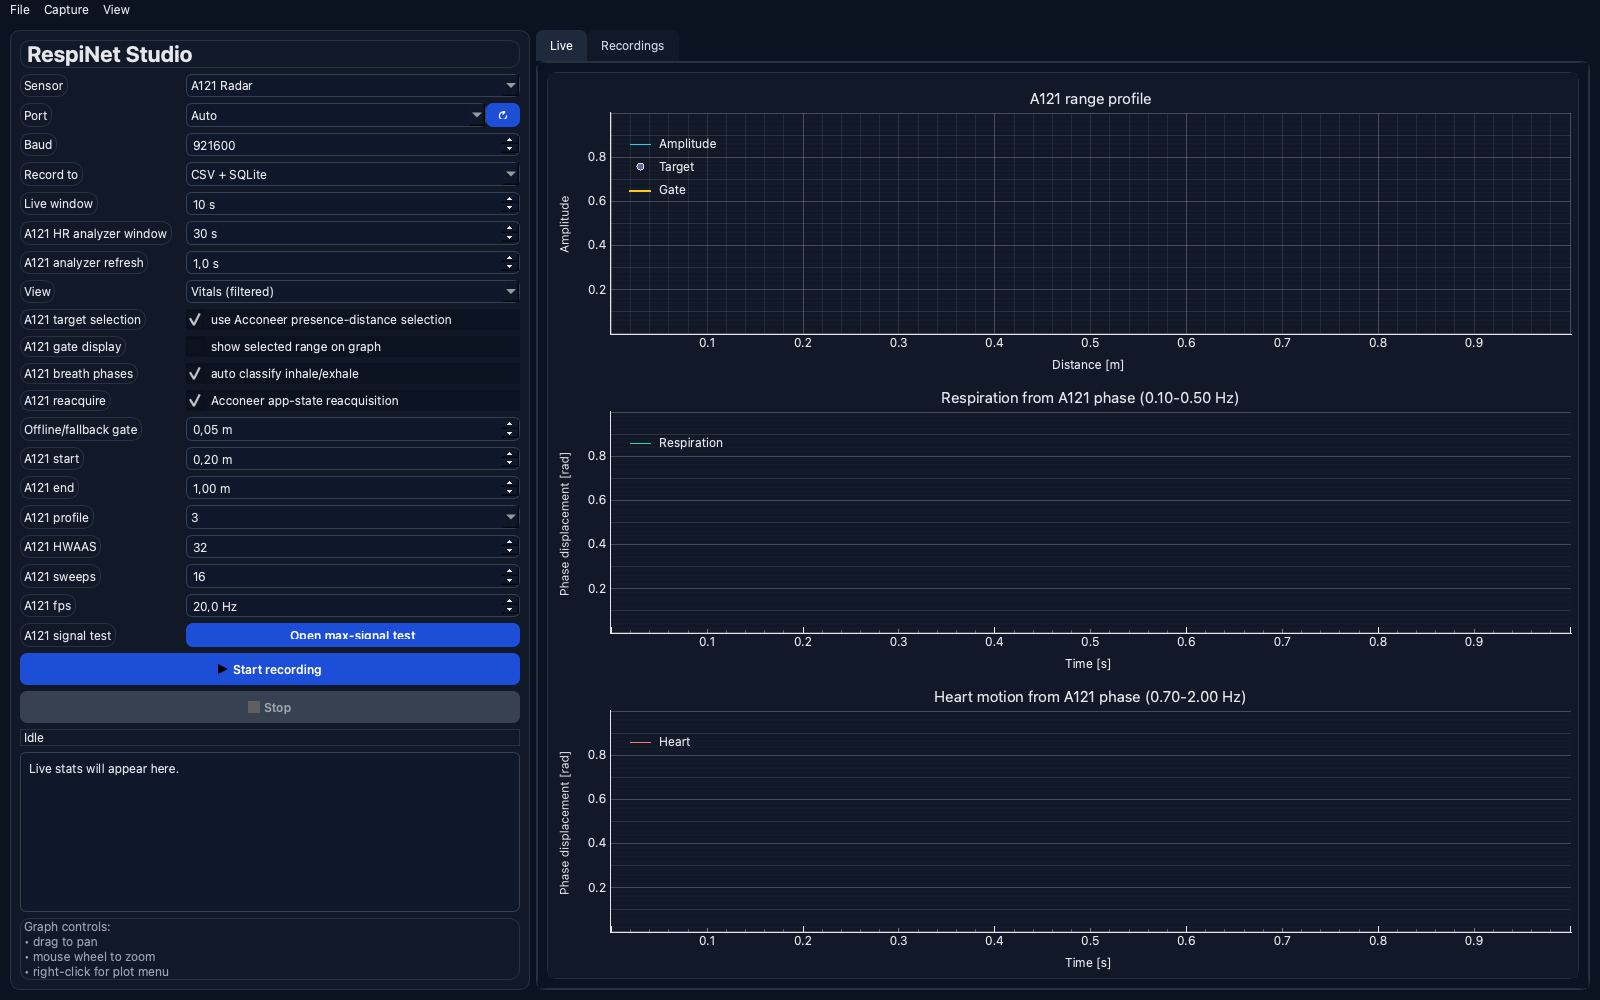
\includegraphics[width=0.95\textwidth]{respi_a121_live_ui.png}
    \caption[Widok A121 aplikacji desktopowej]{Widok toru A121 w~aplikacji
    \emph{RespiNet Sensor Studio}. Interfejs grupuje ustawienia odległości,
    HWAAS, liczbę przemiatań, częstość ramek i~wybór bramki po lewej stronie;
    po prawej przygotowuje trzy wykresy używane podczas akwizycji na żywo.}
    \label{fig:desktop-a121-live}
\end{figure}

\begin{figure}[H]
    \centering
    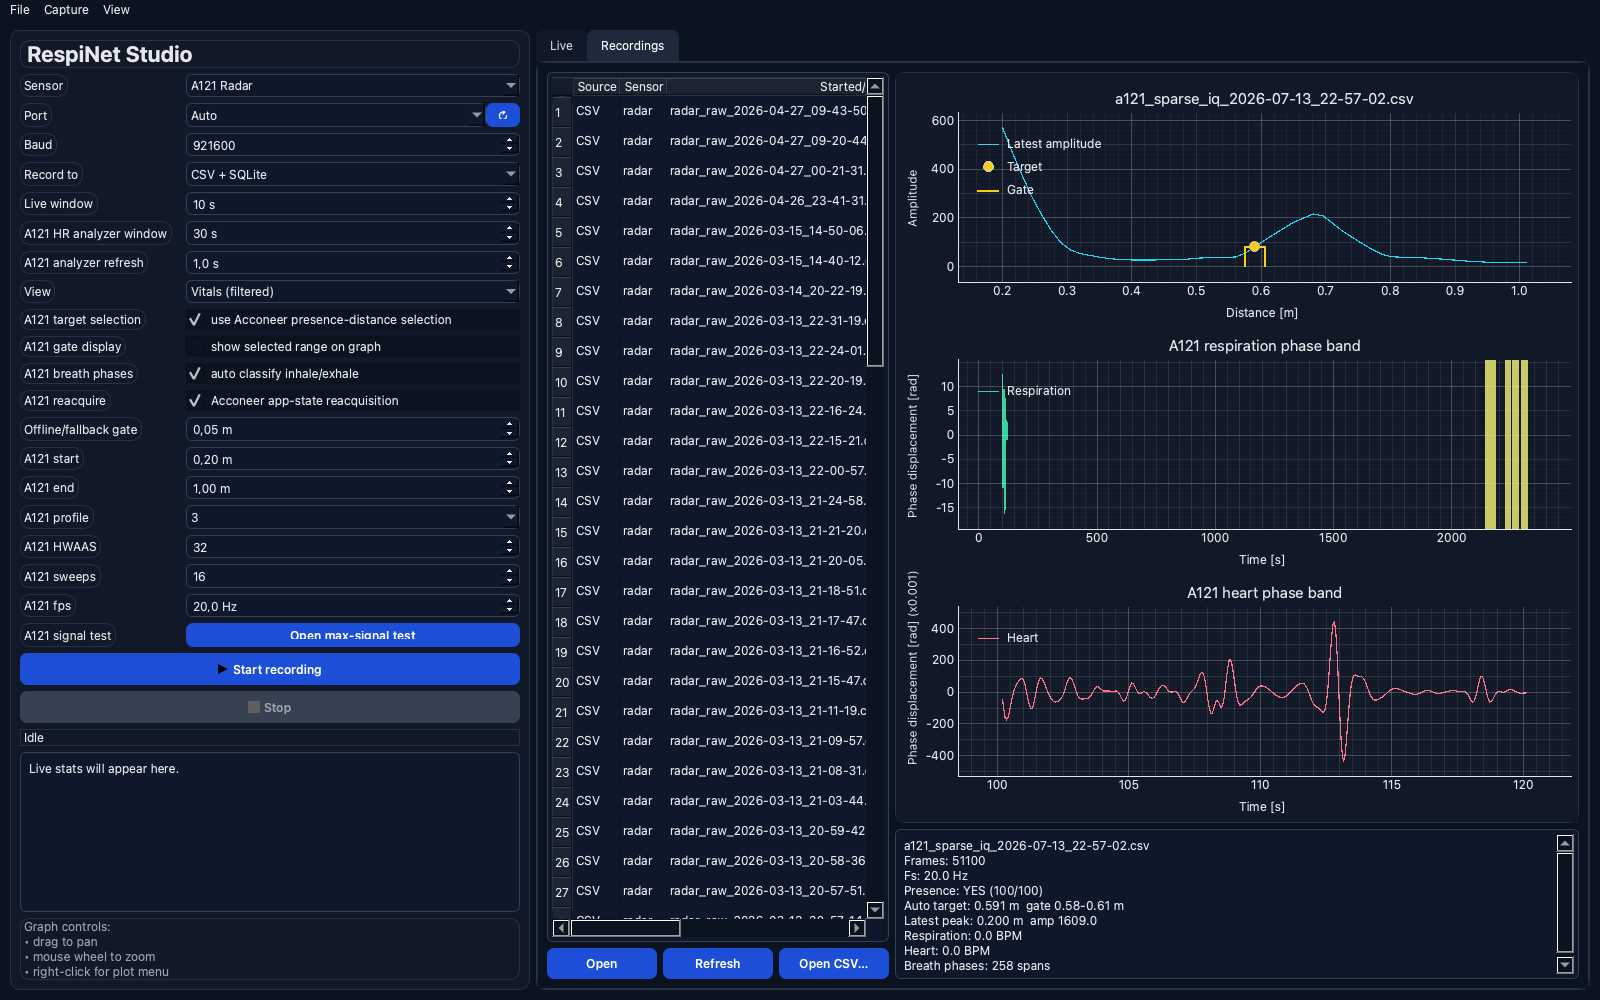
\includegraphics[width=0.95\textwidth]{respi_a121_history_ui.png}
    \caption[Historia nagrań A121 w aplikacji desktopowej]{Przeglądarka
    nagrań aplikacji desktopowej po otwarciu rzeczywistego pliku Sparse IQ
    A121. Tabela po lewej pozwala wybrać źródło, a~wykresy po prawej pokazują
    profil amplitudy z~bramką oraz składowe oddechową i~sercową.}
    \label{fig:desktop-historia}
\end{figure}

\subsection{Programowy przewodnik oddechu}
\label{sec:programowy-przewodnik-oddechu}

Do powtarzalnych prób fazowych przygotowano funkcję programowego przewodnika
oddechu. Interfejs wyświetla dużą komendę
\emph{wdech}, \emph{wydech}, \emph{wstrzymaj oddech} albo \emph{oddychaj
swobodnie}; zmianę sygnalizuje także dźwiękiem. Harmonogram nie jest zaszyty
w~pliku czujnika. Dla każdej komendy zapisywany jest rodzaj, czas początku
i~końca względem startu nagrania oraz odpowiadający czas hosta. Pozwala to
nakładać fazy na równoczesne strumienie różnych urządzeń bez wnioskowania
o~nich z~samego kształtu sygnału.

W~próbach 90-sekundowych stosowano \SI{10}{s} oddechu swobodnego, 7~cykli
wdech \SI{2}{s}--wydech \SI{3}{s}, \SI{15}{s} wstrzymania po wydechu oraz
6~kolejnych cykli \SI{2}{s}/\SI{3}{s}. Odpowiada to dokładnie
12~oddechom/min w~częściach sterowanych. Operator może w~dowolnym momencie
przerwać próbę; bieżące pliki są wtedy usuwane zamiast trafiać do zbioru jako
niepełne nagranie.

\todo{Dodać opis implementacji skryptu programowego przewodnika: obsługę obu
radarów, plik komend, manifest oraz odrzucanie niepełnej próby.}

\begin{figure}[H]
    \centering
    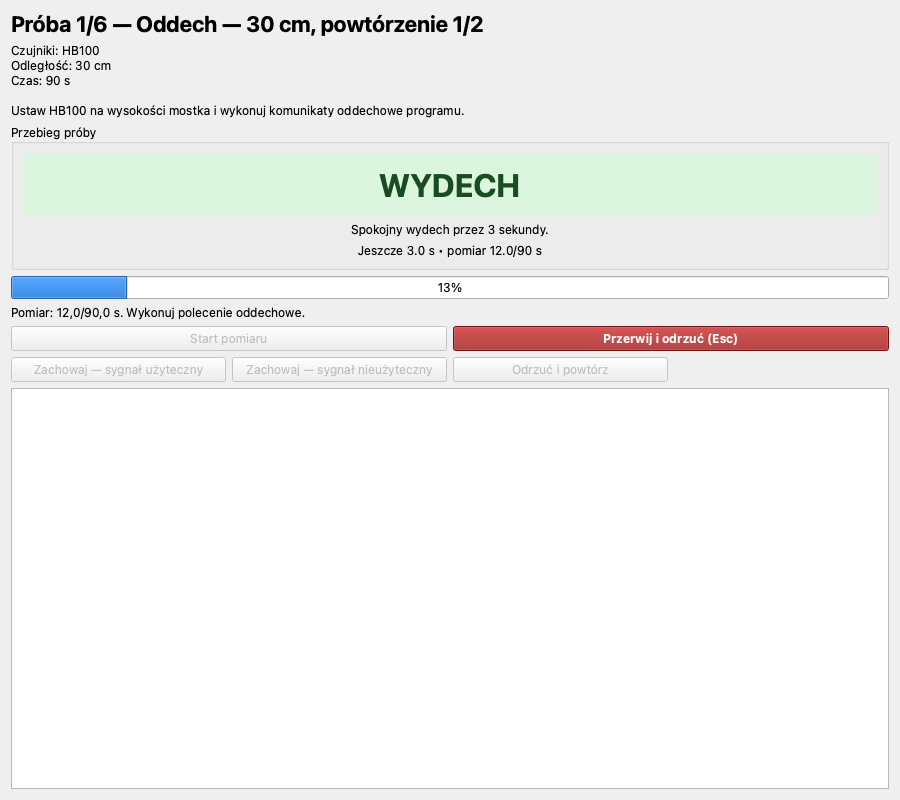
\includegraphics[width=0.72\textwidth]{respi_przewodnik_oddechu_ui.png}
    \caption[Widok programowego przewodnika oddechu]{Programowy
    przewodnik w~fazie \emph{wydechu}. Duży komunikat, pozostały czas oraz
    pasek postępu pozwalają badanemu podążać za protokołem, natomiast wyraźny
    przycisk przerwania zapewnia odrzucenie niepełnego nagrania.}
    \label{fig:programowy-przewodnik-ui}
\end{figure}

Komenda programu jest zamiarem, a~nie bezpośrednim pomiarem fizjologicznym.
Reakcja człowieka i~akwizycja wnoszą opóźnienie, dlatego w~analizach fazowych
znaczniki przesuwa się na podstawie sygnału koherentnego A121. Pierwszy
eksperyment soczewek na dystansach \SI{50}{cm} i~\SI{100}{cm} nie korzystał
z~tego rytmu: przewodnik sterował kolejnością stanowiska, lecz badany oddychał
swobodnie. Pełny harmonogram zastosowano w~retestach wymagających porównania
wdechu, wydechu i~wstrzymania.

\chapter{Eksperymentalne porównanie radarów HB100 i A121}
\label{chap:hb100-a121-pomiar}

Rozdział zestawia oba zbudowane tory dopiero po przedstawieniu ich
architektur oraz algorytmów rekonstrukcji sygnału. Celem nie jest
potraktowanie A121 jako wzorca fizjologicznego, lecz sprawdzenie, jak
architektura jednokanałowego radaru CW i~dostęp do zespolonych danych I/Q
wpływają na trzy odrębne zadania: wykrycie aktywności oddechowej,
oszacowanie jej okresowości oraz rozróżnienie wdechu i~wydechu.

We wszystkich krótkich badaniach radarowych wykonywanych na jawie w~tej pracy
(porównanie HB100--A121 oraz eksperymenty soczewek) badany był bez koszulki,
z~odsłoniętym torsem. Między anteną a~klatką nie było więc warstwy odzieży;
zapisano tym samym warunek referencyjny bez dodatkowego tłumienia i~zmiany
odbicia przez materiał. Warunek ten nie dotyczy całonocnych pomiarów przez
kołdrę opisanych dalej.

\section{Stanowisko i protokół}

Oba radary rejestrowały ten sam oddech równocześnie. Środki apertur HB100
i~A121 znajdowały się obok siebie na wysokości mostka, w~odległości
\SI{15}{cm} mierzonej poprzecznie między ich środkami. Osie ustawiono z~tym
samym nachyleniem względem tułowia. Dla każdego dystansu położenie stanowiska
korygowano tak, aby odległość od obu radarów do tułowia była taka sama
i~wynosiła nominalnie \SI{30}{cm}, \SI{60}{cm}, \SI{100}{cm} albo ---
w~pojedynczym reteście granicznym --- \SI{150}{cm}.

Odległość i~zgodność ustawienia kątowego kontrolowano tym samym dalmierzem
laserowym MILESEEY~D2 w~wariancie \SI{40}{m}, który wykorzystano również
w~eksperymencie soczewek. Odczyt laserowy służył do ustawienia dystansu,
a~poziomnice pęcherzykowe urządzenia i~położenie plamki na klatce --- do
powtarzalnego ustawienia kierunku osi. Nie był to laboratoryjny pomiar
trójwymiarowego kąta powierzchni klatki, lecz kontrola, że oba radary
obserwują tułów z~porównywalnej geometrii \cite{mileseey_d2}.

A121 wyposażono celowo w~płaską pokrywę. Nie skupia ona wiązki i~zapewnia
najszersze pole widzenia spośród używanych wariantów, dzięki czemu jego
pokrycie kątowe jest bardziej porównywalne z~szeroką wiązką HB100 niż
w~przypadku soczewki hiperbolicznej albo FZP. Pola widzenia nadal nie są
identyczne, a~rozstaw \SI{15}{cm} oznacza obserwację częściowo różnych
fragmentów tułowia. Porównanie dotyczy więc odpowiedzi dwóch kompletnych
torów na ten sam akt oddechowy, a~nie kalibracji punkt-do-punktu.

Elementy stanowiska i~sposób ich niezależnego zamocowania przedstawiono na
rys.~\ref{fig:hb100-a121-stanowisko}. Dokładny rozstaw, dystans do tułowia
i~nachylenie ustawiano dopiero przed każdą próbą zgodnie z~opisaną procedurą.

\begin{figure}[H]
    \centering
    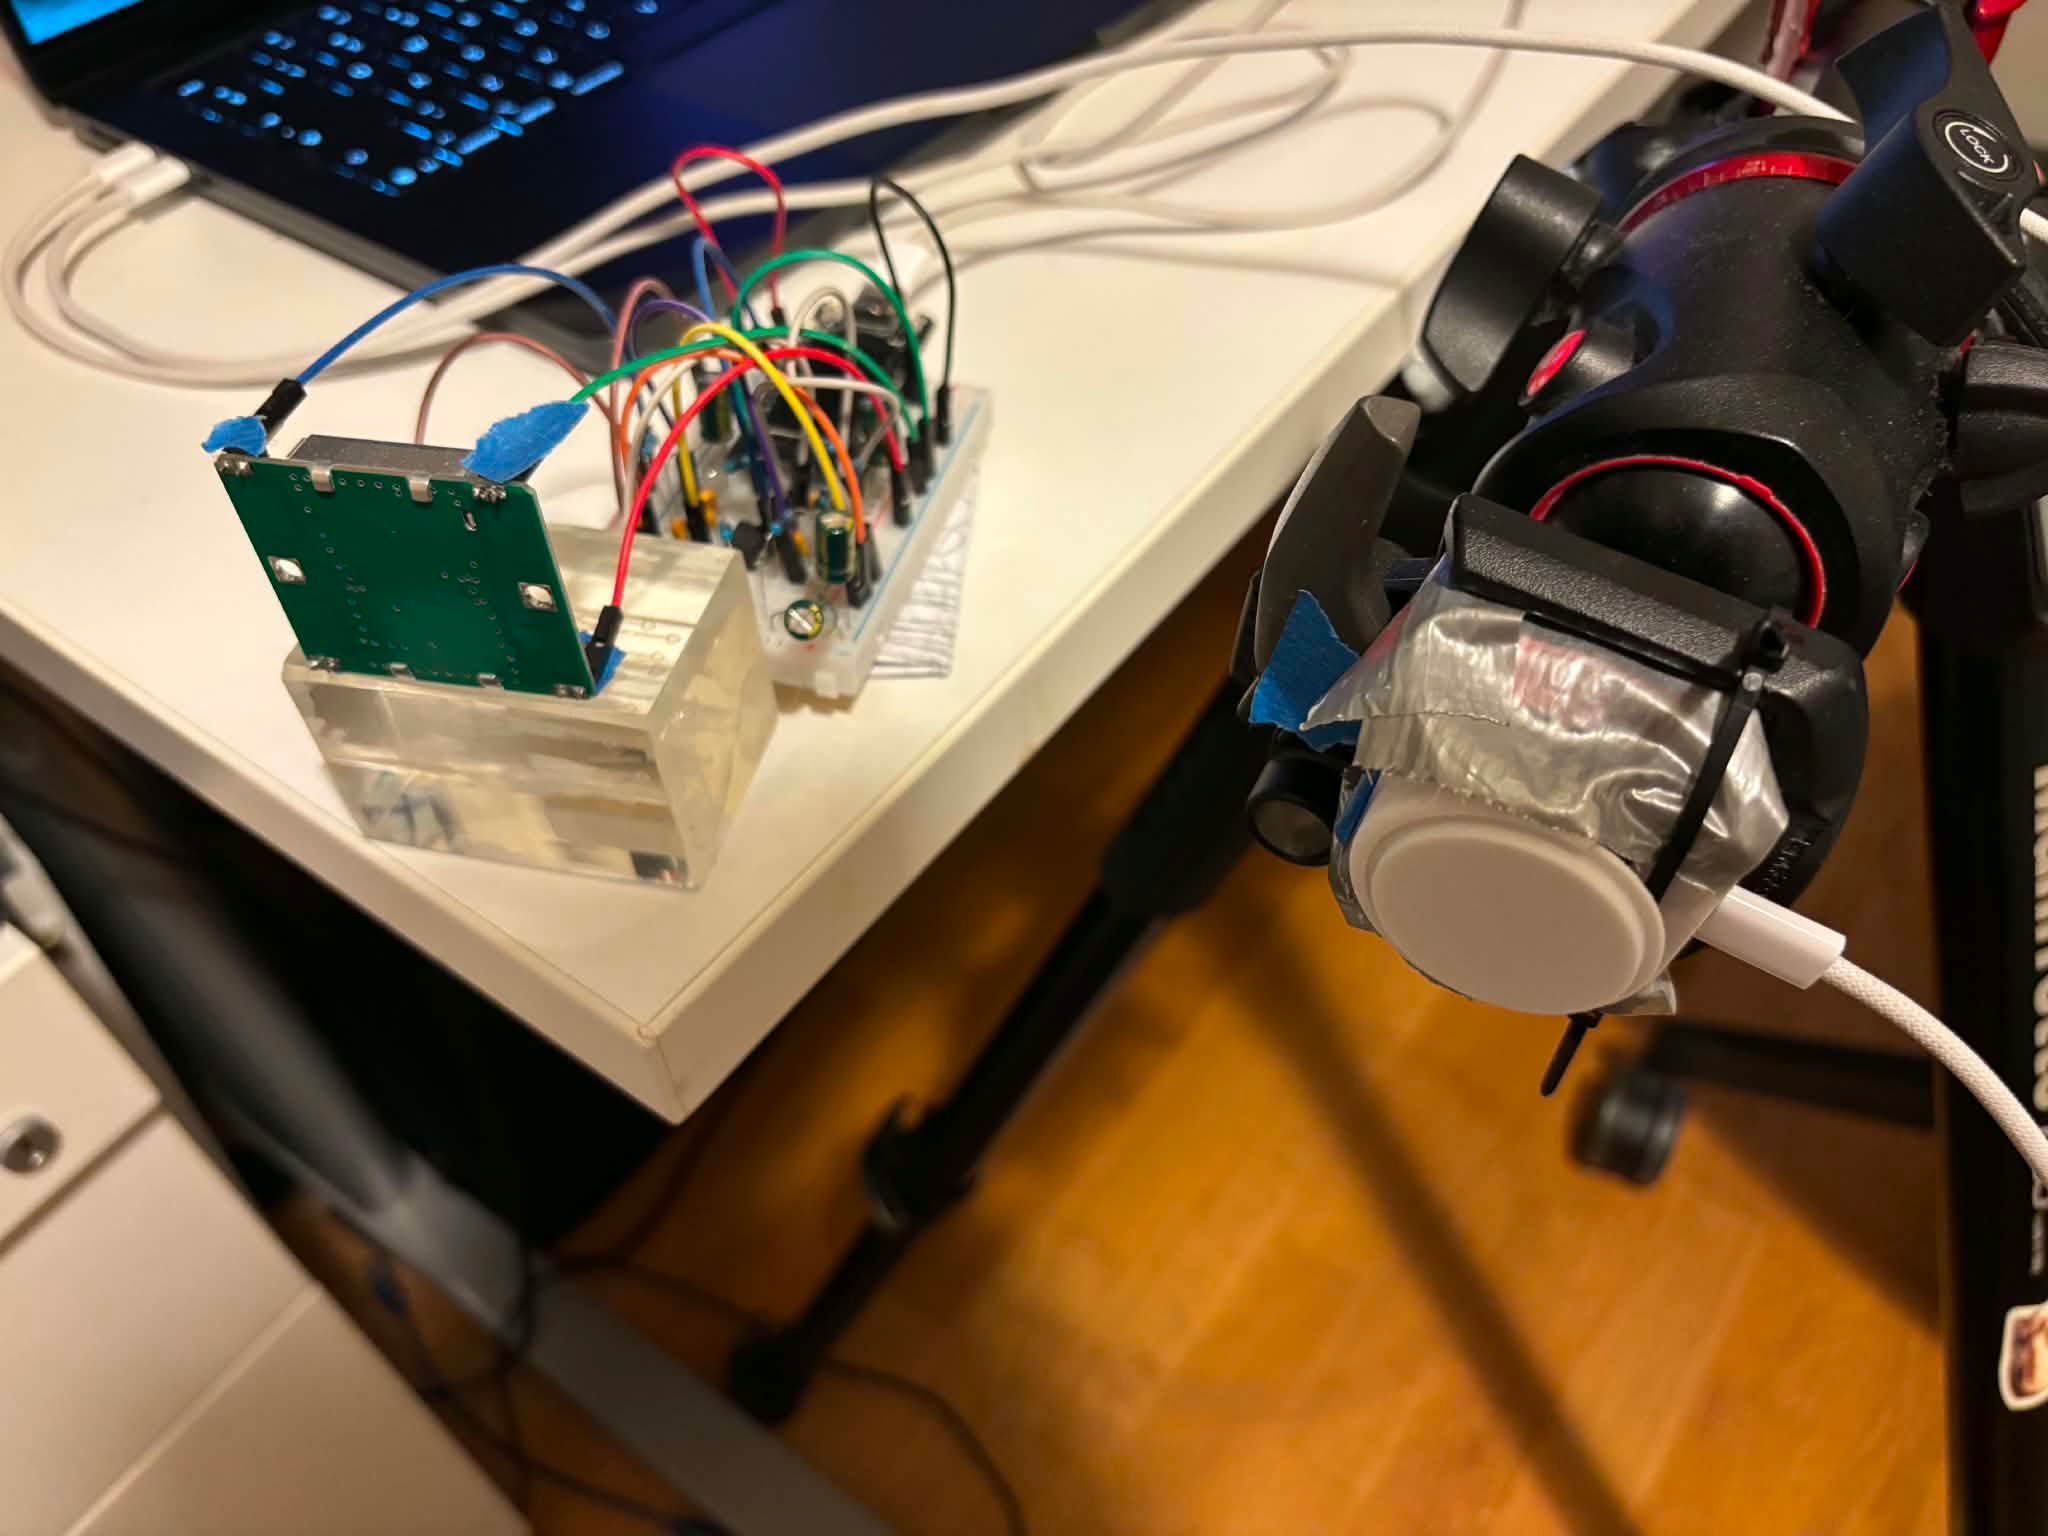
\includegraphics[width=0.84\textwidth]{stanowisko_hb100_a121_porownanie.png}
    \caption[Stanowisko porównania radarów HB100 i A121]{Elementy stanowiska
    równoczesnego porównania radarów: po lewej moduł HB100 z~analogowym
    front-endem na płytce stykowej, a~po prawej A121 z~płaską pokrywą,
    zamocowany na głowicy statywu Manfrotto. Przed pomiarem położenie obu
    czujników korygowano do geometrii opisanej w~tekście (fotografia własna).}
    \label{fig:hb100-a121-stanowisko}
\end{figure}

Wykonano po dwa nagrania na każdym z~trzech dystansów. Każde trwało
\SI{90}{s}. A121 pracował z~profilem~3, HWAAS~32, ośmioma przemiatanami
na ramkę i~częstością \SI{20}{Hz}; zakres bramek obejmował nominalną
pozycję klatki z~marginesem około \SI{50}{cm}. HB100 rejestrowano
z~częstością \SI{250}{Hz} przez tor opisany w~sekcji~\ref{sec:frontend}.

Sekwencję oddechową prowadził program komunikatów oddechowych opisany w~sekcji
\ref{sec:programowy-przewodnik-oddechu}. Po \SI{10}{s} oddechu swobodnego następowało
7~cykli: wdech \SI{2}{s} i~wydech \SI{3}{s}, następnie \SI{15}{s}
wstrzymania po wydechu oraz 6~kolejnych cykli \SI{2}{s}/\SI{3}{s}. Zadana
częstość wynosiła \SI{0.20}{Hz}, czyli 12~oddechów/min. Każdy plik czujnika
otrzymał czas hosta, a~osobny plik zawierał początek i~koniec każdej komendy.
A121 nie jest w~tym porównaniu wzorcem fizjologicznym; pełni rolę drugiego,
koherentnego toru obserwującego ten sam ruch.

W~odcinkach sterowanych badany wykonywał pełne, wyraźnie pogłębione oddechy,
o~większej amplitudzie ruchu klatki piersiowej niż przy zwykłym, swobodnym
oddychaniu. Jest to celowo korzystne pobudzenie do sprawdzenia granic toru
HB100, a~nie próba odwzorowania oddechu spoczynkowego ani snu. Wnioski
o~częstości odnoszą się więc do takiego, kontrolowanego ruchu; nie należy
przenosić ich bezpośrednio na płytszy oddech naturalny.

Po serii podstawowej wykonano pojedynczy retest na \SI{150}{cm}, zachowując
ten sam protokół, rozstaw radarów i~płaską pokrywę A121. Jego celem było
sprawdzenie praktycznej granicy informacji uzyskiwanej z~jednokanałowego
HB100, a~nie wyznaczenie pełnej krzywej zasięgu: nie ma drugiego powtórzenia
ani randomizacji. Płaską pokrywę pozostawiono celowo dla porównywalnego pola
widzenia z~HB100. Na takim dystansie nie daje ona zysku skupiającego soczewki
hiperbolicznej ani FZP, dlatego wynik A121 nie jest demonstracją maksymalnego
zasięgu tego czujnika z~optyką skupiającą.

Wszystkie sześć par było kompletne. W~każdym nagraniu HB100 zapisano od
22502 do 22510 próbek, a~A121 1801 ramek. Nie odrzucono ani jednej ramki A121,
nie wystąpiły też niepoprawne wiersze transmisji HB100. Rzeczywiste medianowe
częstości wyniosły odpowiednio \SI{250.0}{Hz} i~\SI{20.0}{Hz}.

\section{Kontrola wzajemnych zakłóceń}

Przed pomiarem badanego wykonano trzy \SI{30}{s} kontrole pustej, nieruchomej
sceny: A121 przy wyłączonym HB100, oba radary równocześnie oraz HB100 przy
zatrzymanym A121. Dla A121 porównano medianę po bramkach z~wyraźnym echem:
znormalizowany RMS zmian zespolonego IQ wyniósł 0,16449 dla A121 pracującego
samodzielnie i~0,16430 przy włączonym HB100 (zmiana $-0{,}12\%$). RMS fazy
w~paśmie \SIrange{0.10}{0.60}{Hz} wyniósł odpowiednio 0,04062 i~0,03975~rad
(zmiana $-2{,}16\%$). Oba zapisy miały po 601 ramek i~nie zawierały strat.

Dla HB100 RMS napięcia po usunięciu trendu wyniósł \SI{5.615}{mV} przy pracy
samodzielnej i~\SI{4.780}{mV} podczas równoczesnej pracy A121, czyli nie
wzrósł, lecz zmalał o~\SI{1.40}{dB}. W~tej krótkiej kontroli nie stwierdzono
zatem mierzalnego wzajemnego zakłócania torów. Jest to wynik dla jednego
ustawienia i~pustej sceny, a~nie dowód odporności w~każdej geometrii.

\section{Rekonstrukcja i synchronizacja sygnałów}

Dla A121 wybrano stały zestaw trzech bramek, który najczęściej wskazywała
referencyjna maszyna stanów Acconeer. Takie użycie bramki modalnej zapobiega
skokowi fazy, gdy algorytm w~trakcie nagrania ponownie wybiera cel. Fazę IQ
rozpleciono, usunięto trend liniowy, uśredniono z~wagami proporcjonalnymi do
medianowej amplitudy bramek i~przeliczono na przemieszczenie. Składową
oddechową A121 ograniczono filtrem zerofazowym do
\SIrange{0.10}{0.50}{Hz}.

Napięcie HB100 wyrównano do siatki \SI{100}{Hz} i~zastosowano filtr
zerofazowy \SIrange{0.10}{0.70}{Hz}. Szersza górna granica celowo zachowuje
drugą i~trzecią harmoniczną zadanego rytmu. Opóźnienia komend nie dopasowywano
osobno do HB100. Dla każdego nagrania wyznaczono je wyłącznie z~korelacji
sygnału A121 z~trójkątnym wzorcem \SI{2}{s}/\SI{3}{s}; otrzymano
\SIrange{0.250}{0.550}{s}, z~medianą \SI{0.325}{s}. Obejmuje to reakcję
badanego i~opóźnienia akwizycji. O~tę wartość przesunięto tła komend na
rys.~\ref{fig:hb100-a121-etapy}.

Oba tory poddano tej samej procedurze: dla każdego wybrano jedną polaryzację
maksymalizującą zgodność z~pierwszym blokiem sterowanym i~nie zmieniano jej już
w~drugim bloku. Procedura ta działa jednak na obu torach zupełnie inaczej i~ta
różnica jest sama w~sobie wynikiem.

Dla A121 kalibracja okazała się operacją pustą. Znak jego fazy nie jest umowny,
lecz wynika z~konwencji toru omówionej w~sekcji~\ref{sec:model-sygnalu}:
we~wszystkich siedmiu nagraniach wybrana polaryzacja była dodatnia,
a~korelacja surowego, nieskorygowanego przemieszczenia ze wzorcem wynosiła już
$0{,}909$--$0{,}959$. Gdyby kalibrację całkowicie pominąć, wyniki A121 byłyby
identyczne. Dla HB100 przeciwnie --- polaryzację odwrócono w~każdym z~siedmiu
nagrań, a~korelacja przed korektą mieściła się w~zakresie
$-0{,}514$--$-0{,}171$, czyli była słaba niezależnie od przyjętego znaku.

Jest to zatem celowo łagodny test HB100, a~nie wyrównanie szans: A121 nie
korzysta z~tej ulgi, natomiast HB100 dostaje jednorazową kalibrację znaku
i~mimo niej sprawdzany jest tylko pod kątem tego, czy raz ustalone mapowanie
przetrwa wstrzymanie oddechu.

Zestawienie przykładowych przebiegów surowych i~po filtracji umieszczono
dopiero po opisie estymatora rytmu (rys.~\ref{fig:hb100-a121-etapy}), aby
odczyt przebiegów odnosił się już do ich znaczenia fizycznego i~ograniczeń
jednokanałowego HB100.

\section{Pomocniczy estymator rytmu z jednokanałowego HB100}
\label{sec:hb100-rytm}

Bezpośrednie porównanie dwóch przebiegów wymaga rozdzielenia ich znaczenia
fizycznego. Dla A121 fazę zespolonego IQ można rozpleść i~przeliczyć na
przemieszczenie klatki. W~torze HB100 mieszacz udostępnia pojedyncze,
rzeczywiste napięcie IF. Dla ruchu o~stałej prędkości radialnej jego
częstotliwość Dopplera jest proporcjonalna do prędkości
(równanie~\eqref{eq:hb100-doppler}), lecz podczas oddechu chwilowa wartość
napięcia IF jest nieliniową funkcją całkowitej fazy echa
(równanie~\eqref{eq:cw-baseband}). Jej skala zależy więc od fazy statycznej
i~nie może być bezpośrednio przeliczona na milimetry tak jak faza A121.
Dla modelu~\eqref{eq:cw-baseband} różniczkowanie daje
\begin{equation}
  \frac{\mathrm{d}b(t)}{\mathrm{d}t}
  =-A\sin\!\left(\frac{4\pi}{\lambda}[d_0+x(t)]+\varphi_0\right)
  \frac{4\pi}{\lambda}\frac{\mathrm{d}x(t)}{\mathrm{d}t}.
  \label{eq:hb100-pochodna-if}
\end{equation}
Nieznany czynnik sinusoidalny zależy od fazy statycznej, zmienia znak i~zanika
w~punktach zerowych. W~rezultacie pochodna napięcia IF nie daje stabilnej
estymaty prędkości, a~całkowanie napięcia ani jego pochodnej nie odtwarza
przemieszczenia. Dopiero para kanałów I/Q pozwoliłaby odzyskać ciągłą fazę
i~jej znak.

Zamiast tego opracowano estymator \emph{konsensusu harmonicznych}, którego
wynikiem jest wyłącznie częstość powtarzalnej modulacji. Dla co najmniej
\SI{20}{s} ustabilizowanego okna HB100 przeszukuje kandydatów
$f\in\SIrange{0.10}{0.30}{Hz}$ i~oblicza
\begin{equation}
  S(f)=\sum_{k=1}^{3}\hat a_k^2(kf),\qquad
  \hat f=\mathop{\mathrm{arg\,max}}_f S(f),
  \label{eq:hb100-harmonic-consensus}
\end{equation}
gdzie $\hat a_k(kf)$ jest amplitudą sinusoidy o~częstości $kf$, dopasowaną
metodą najmniejszych kwadratów do wyrównanego czasowo i~pozbawionego trendu
napięcia HB100. Energia podstawy oraz drugiej i~trzeciej harmonicznej jest
więc składana do wspólnego kandydata zamiast wybierania najsilniejszego piku
widma.

Pomysł nie jest nowy: jest to wariant \emph{sumy harmonicznej}, metody
opracowanej pierwotnie do wyznaczania częstotliwości podstawowej mowy
\cite{noll1970}. Schroeder wykazał, że częstość sygnału okresowego,
\emph{którego składowa podstawowa jest niedostępna pomiarowo}, można odzyskać
z~częstotliwości jego wyższych harmonicznych \cite{schroeder1968} --- czyli
rozwiązał dokładnie ten problem, który w~torze HB100 tworzy nieliniowa
demodulacja fazy. Nowy jest tu wyłącznie kontekst: przeniesienie metody
z~analizy dźwięku na jednokanałowy radar CW oraz dobór bramek jakości do tego
zastosowania.

Amplitudę wyznacza się dopasowaniem najmniejszych kwadratów w~dowolnie wybranej
częstotliwości, a~nie odczytem prążka FFT. Pozwala to zagęścić siatkę
kandydatów do \SI{0.001}{Hz}, podczas gdy rozdzielczość prążkowa okna
\SI{30}{s} wynosiłaby zaledwie około \SI{0.033}{Hz}, czyli około
2~oddechów/min. Zabieg ten usuwa kwantyzację odczytu, lecz nie zmienia
fizycznej zdolności rozdzielczej: dwóch tonów odległych o~mniej niż $1/T$
nadal nie da się rozróżnić. Precyzyjna estymacja dotyczy tu pojedynczego,
dobrze odseparowanego składnika, co jest typowym przypadkiem stosowalności
najmniejszych kwadratów w~dziedzinie częstotliwości \cite{vanderplas2018}. Wynik jest publikowany tylko, gdy co najmniej dwie składowe wnoszą po
minimum 5\% energii, najlepszy wynik przewyższa o~co najmniej 5\% kandydata
oddalonego o~\SI{0.035}{Hz}, a~jego wynik jest co najmniej dwukrotnie większy
od mediany $S(f)$. W~przeciwnym przypadku algorytm zwraca brak estymaty, a~nie
zgadywaną częstość.

Algorytm wykorzystuje wyłącznie próbki HB100; A121 nie wybiera ani nie
koryguje $\hat f$. W~tym eksperymencie czasy komend służą wyłącznie do
wydzielenia dwóch niezależnie ocenianych bloków. Testy jednostkowe obejmują
syntetyczny sygnał z~ukrytą podstawą i~silnymi harmonicznymi oraz sygnał
jednoskładowy, który jest celowo oznaczany jako niejednoznaczny. Metoda nie
rozstrzyga kierunku wdech--wydech i~nie może być użyta do rekonstrukcji
przemieszczenia ani do samodzielnego rozpoznawania bezdechu.

\begin{figure}[H]
    \centering
    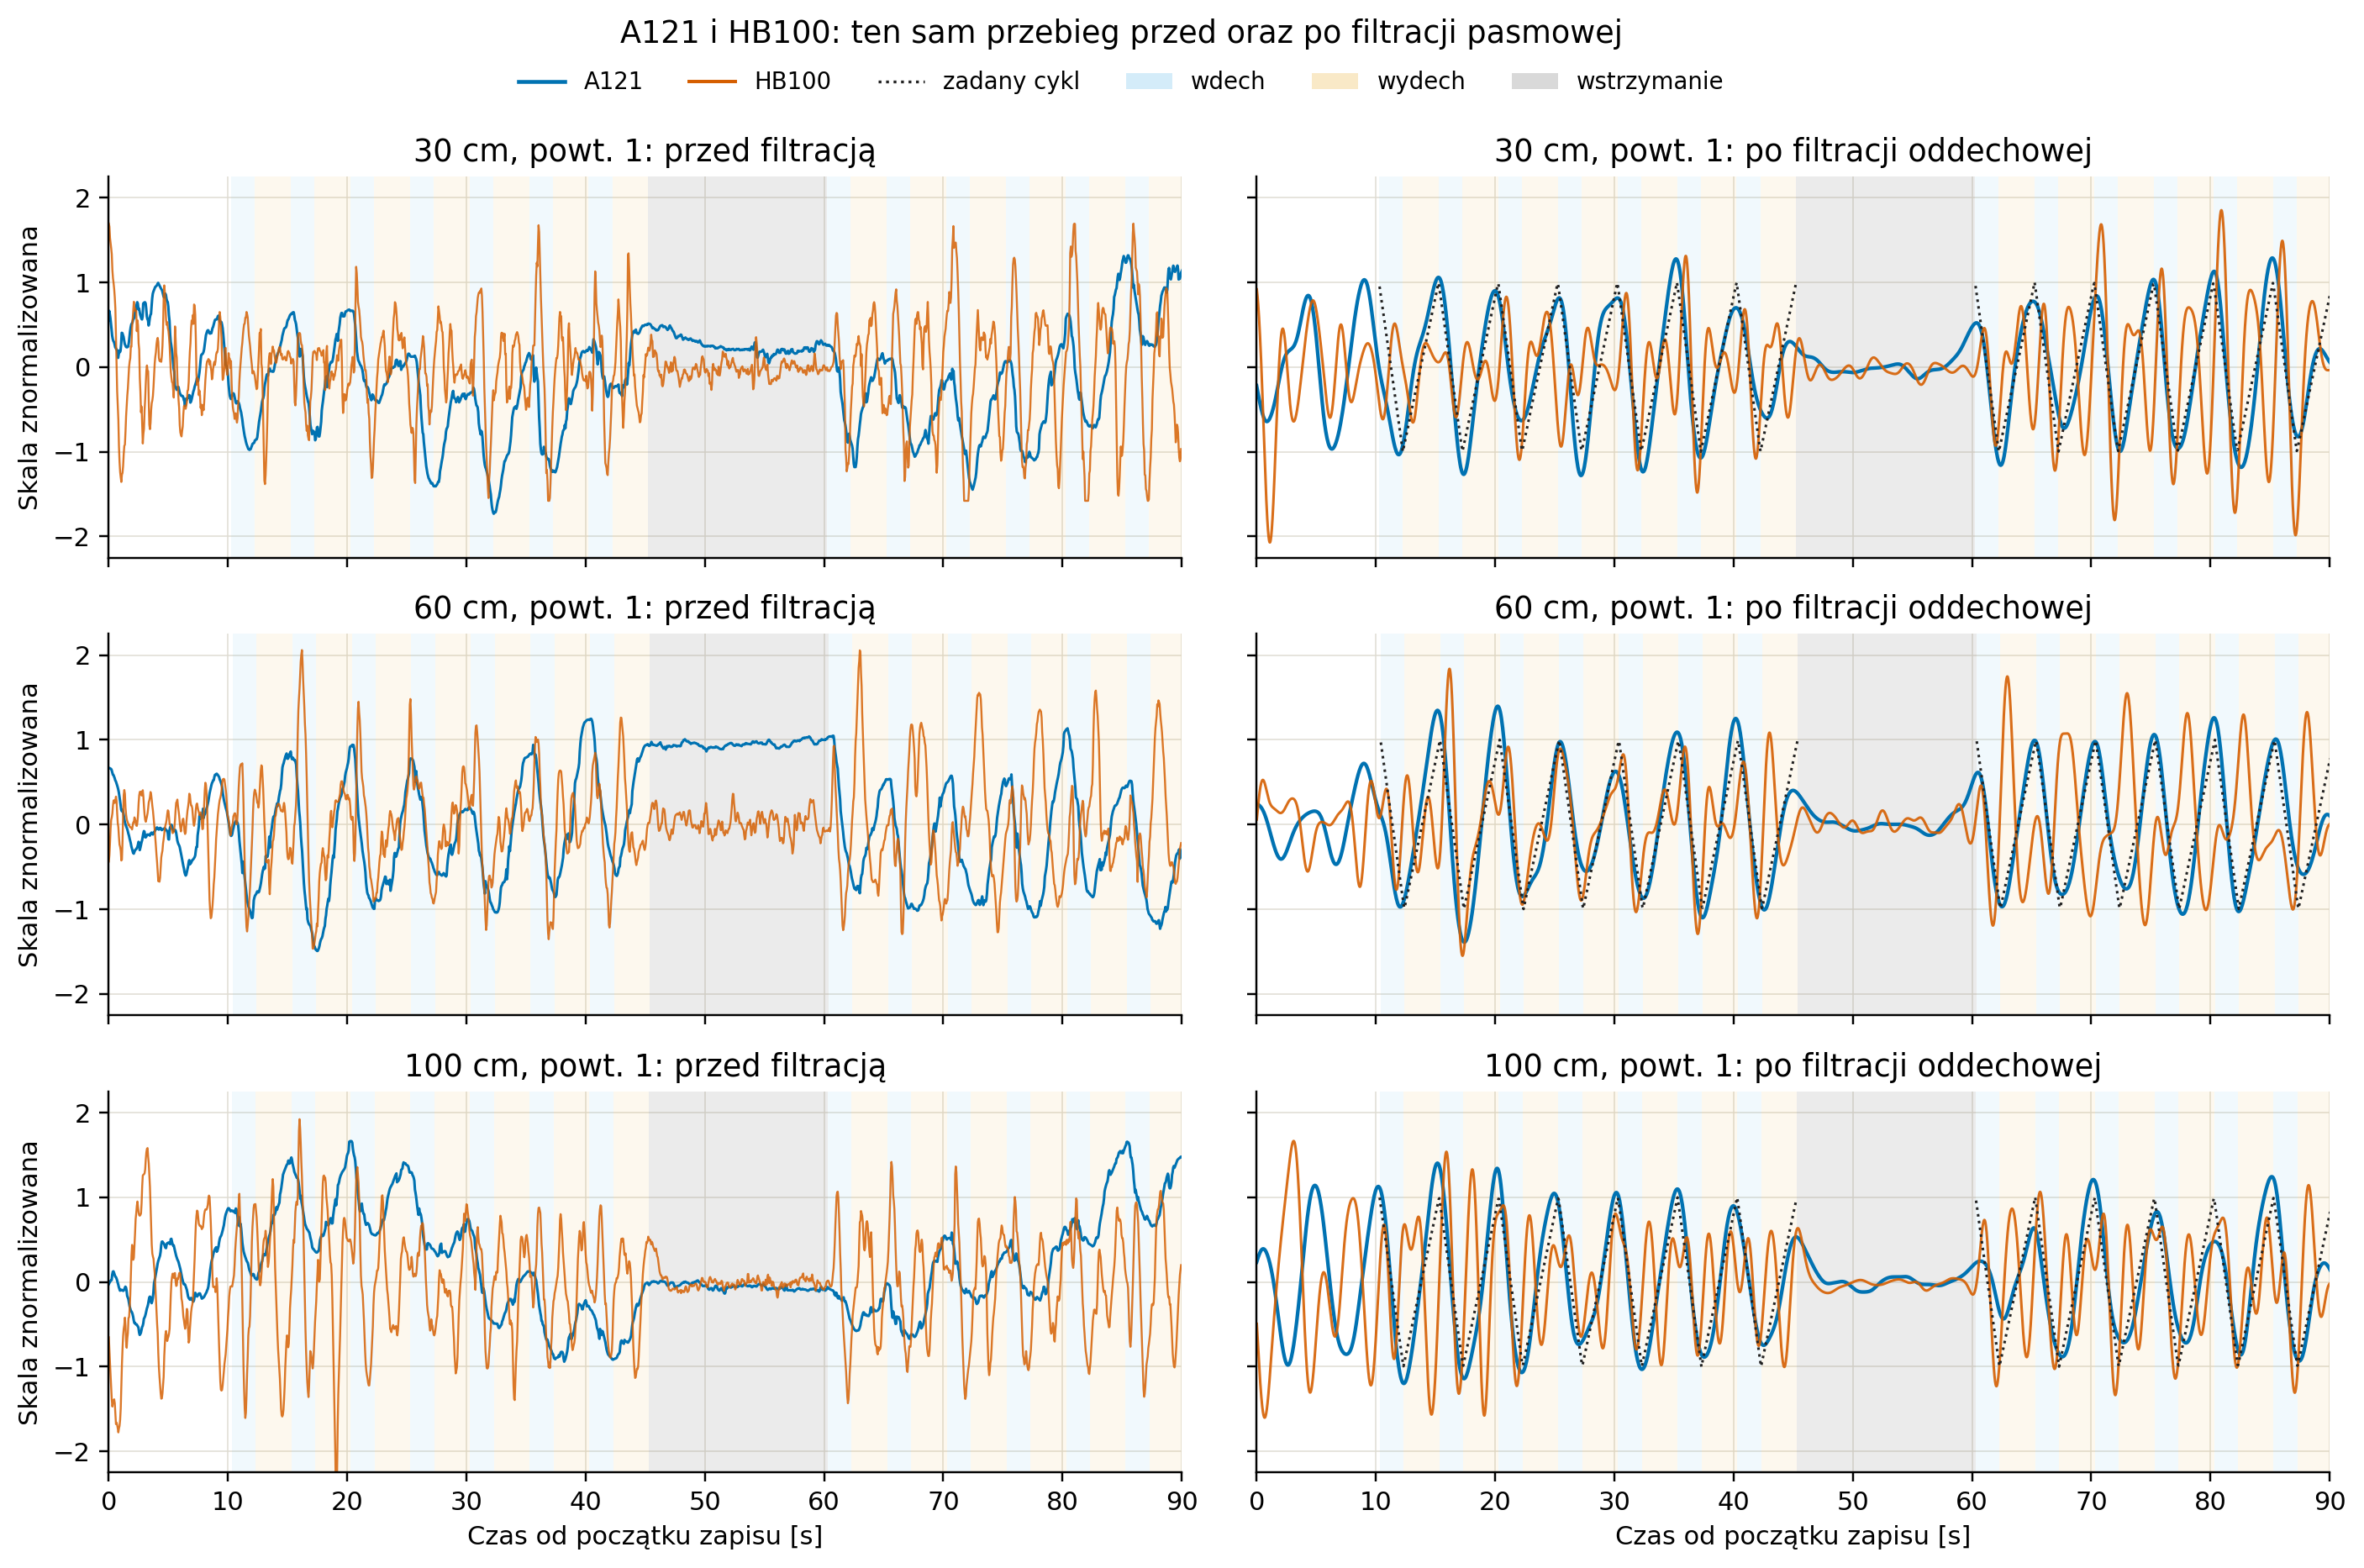
\includegraphics[width=\textwidth]{hb100_a121_etapy_30_100.png}
    \caption[Przebiegi A121 i HB100 przed oraz po filtracji]{Przykładowe
    pierwsze powtórzenie na \SI{30}{cm}, \SI{60}{cm} i~\SI{100}{cm}.
    Lewa kolumna zawiera przebiegi przed filtracją oddechową: rozplecioną fazę
    IQ A121 oraz napięcie ADC HB100. Prawa pokazuje te same zapisy po
    filtracji pasmowej; dla A121 jest to przemieszczenie z~fazy IQ, a~dla
    HB100 napięcie IF. Sygnały znormalizowano osobno, zatem rysunek porównuje
    czas i~kształt, nie amplitudę. Niebieskie, pomarańczowe i~szare pola
    odpowiadają po korekcie opóźnienia odpowiednio wdechowi, wydechowi
    i~wstrzymaniu. Drugie powtórzenia uwzględniają tabele i~rysunek
    rytmu~\ref{fig:hb100-a121-rytm-dystanse}.}
    \label{fig:hb100-a121-etapy}
\end{figure}

Dla porównania rytmu z~A121 w~tych samych oknach wyznaczono na jego
zrekonstruowanym przemieszczeniu najsilniejszy pik w~paśmie
\SIrange{0.10}{0.30}{Hz}. Jest to niezależna, prosta estymata pomocnicza:
nie koryguje ona wyniku HB100 ani nie zmienia jego kryteriów akceptacji.

\section{Wyniki i interpretacja}

Tabela~\ref{tab:hb100-a121-wyniki} rozdziela wykrycie ruchu od zachowania fazy
cyklu. $r_{A,2}$ i~$r_{H,2}$ są korelacjami z~zadanym przebiegiem w~drugim
bloku. $Q_{A,2}$ i~$Q_{H,2}$ oznaczają zrównoważony odsetek próbek, dla których
znak pochodnej sygnału zgadza się z~kierunkiem wdech/wydech; pominięto po
\SI{0.30}{s} przy każdej granicy komendy. Nie jest to wynik klasyfikatora
uczonego, lecz opisowa miara monotoniczności i~stabilności kierunku.

Ta sama liczba znaczy jednak dla obu torów co innego i~warto to powiedzieć
wprost. Dla A121 mierzy ona rzeczywisty kierunek ruchu klatki, bo faza IQ
niesie znak przemieszczenia (sekcja~\ref{sec:model-sygnalu}). Dla HB100 jest
natomiast \emph{testem naiwnego założenia}, że rzeczywiste napięcie IF
zachowuje się jak przemieszczenie. Model~\eqref{eq:cw-baseband} przewiduje, że
założenie to musi zawieść: zgodnie z~równaniem~\eqref{eq:hb100-pochodna-if}
znak pochodnej napięcia jest znakiem $\mathrm{d}x/\mathrm{d}t$ przemnożonym
przez nieznany czynnik $-\sin(\cdot)$, zależny od fazy statycznej celu.
Wartość $Q_H$ nie jest więc miarą jakości, którą HB100 mógłby poprawić lepszym
strojeniem toru --- jest predykcją teoretyczną poddaną sprawdzeniu na trzech
dystansach i~dwóch powtórzeniach. Sens jej pomiaru polega na tym, że
przewidywanie modelu zostaje zweryfikowane danymi, a~nie przyjęte na wiarę.

\begin{table}[H]
\centering
\caption{Porównanie faz cyklu i~zaniku sygnału w~sześciu podstawowych
nagraniach oraz pojedynczym reteście \SI{150}{cm}. $f_{H,1}/f_{H,2}$ to dominująca częstość HB100 w~pierwszym
i~drugim bloku; \emph{hold} jest zmianą RMS HB100 w~środkowych \SI{9}{s}
wstrzymania względem odcinków sterowanych.}
\label{tab:hb100-a121-wyniki}
\footnotesize
\setlength{\tabcolsep}{3.5pt}
\begin{tabular}{@{}rrrrrrrrr@{}}
\toprule
Dyst. [cm] & Powt. & $\delta$ [s] & $r_{A,2}$ & $r_{H,2}$ & $Q_{A,2}$ [\%] & $Q_{H,2}$ [\%] & $f_{H,1}/f_{H,2}$ [Hz] & Hold [dB] \\
\midrule
 30 & 1 & 0,250 & 0,945 &  0,238 & 96,5 & 55,6 & 0,598 / 0,397 & $-18{,}4$ \\
 30 & 2 & 0,550 & 0,957 & $-0{,}098$ & 99,3 & 36,5 & 0,403 / 0,397 & $-23{,}9$ \\
 60 & 1 & 0,375 & 0,955 & $-0{,}543$ & 97,9 & 43,8 & 0,208 / 0,201 & $-18{,}9$ \\
 60 & 2 & 0,350 & 0,915 &  0,040 & 98,6 & 63,7 & 0,409 / 0,397 & $-24{,}6$ \\
100 & 1 & 0,300 & 0,894 &  0,438 & 95,9 & 63,4 & 0,403 / 0,397 & $-24{,}3$ \\
100 & 2 & 0,300 & 0,932 &  0,185 & 97,9 & 62,9 & 0,598 / 0,403 & $-24{,}6$ \\
150 & 1 & 0,375 & 0,910 & $-0{,}299$ & 96,7 & 36,6 & 0,366 / 0,378 & $-15{,}7$ \\
\bottomrule
\end{tabular}
\end{table}

Tabela~\ref{tab:hb100-harmonic-rhythm} sprawdza osobno estymator z~równania
\eqref{eq:hb100-harmonic-consensus} oraz prosty pik rytmu A121 w~tych samych
oknach. Nie zastępuje ona powyższej oceny kierunku: jej celem jest wyłącznie
ustalenie, czy z~nieliniowego napięcia HB100 można odzyskać rytm
kontrolowanego ruchu mimo dominacji harmonicznych.

\begin{table}[H]
\centering
\caption{Sprawdzenie estymatora konsensusu harmonicznych HB100 oraz
porównawczego piku A121 w~14 sterowanych blokach po
\SIrange{29.8}{35.0}{s}. Rytm zadany wynosił \SI{0.20}{Hz}; oddechy były
pełne i~pogłębione. Powtarzaną serię \SIrange{30}{100}{cm} rozdzielono od
pojedynczego retestu \SI{150}{cm}.}
\label{tab:hb100-harmonic-rhythm}
\small
\begin{tabular}{@{}p{8.3cm}r@{}}
\toprule
Metryka & Wynik \\
\midrule
Najsilniejszy pojedynczy pik widma HB100 & \SIrange{0.201}{0.598}{Hz} \\
Seria \SIrange{30}{100}{cm}: $\hat f$ & \SIrange{0.198}{0.204}{Hz} \\
Seria \SIrange{30}{100}{cm}: okna spełniające warunki jakości & 12 / 12 \\
Seria \SIrange{30}{100}{cm}: $S_{\max}/\operatorname{med}S$ & $5{,}7$--$21{,}5$ \\
Seria \SIrange{30}{100}{cm}: $\hat f_A$ z~przemieszczenia A121 & \SIrange{0.195}{0.203}{Hz} \\
Retest \SI{150}{cm}: $\hat f$, blok 1 / blok 2 & \SI{0.190}{Hz} / \SI{0.202}{Hz} \\
Retest \SI{150}{cm}: $S_{\max}/\operatorname{med}S$ & 2,9 / 2,1 (próg 2,0) \\
Retest \SI{150}{cm}: $\hat f_A$, blok 1 / blok 2 & \SI{0.197}{Hz} / \SI{0.197}{Hz} \\
\bottomrule
\end{tabular}
\end{table}

W~powtarzanej serii \SIrange{30}{100}{cm} wszystkie 12 bloków spełniło
warunki jakości, a~estymaty \SIrange{0.198}{0.204}{Hz} pozostały blisko
zadanego rytmu. W~tych samych oknach pik z~przemieszczenia A121 wyniósł
\SIrange{0.195}{0.203}{Hz}; na rys.~\ref{fig:hb100-a121-rytm-dystanse}
obie estymaty pozostają więc przy wzorcu 12~oddechów/min. Różnica pojawia się
w~pewności wyniku HB100: przy \SIrange{30}{100}{cm} profile $S(f)$ mają
wyraźny kandydat, natomiast w~pojedynczym reteście \SI{150}{cm} wynik
\SI{0.190}{Hz} w~pierwszym bloku i~\SI{0.202}{Hz} w~drugim ma marże 2,9
i~2,1, wielokrotnie mniejsze niż 5,7--21,5 w~serii krótkodystansowej. Piki
A121 w~tym reteście wyniosły po \SI{0.197}{Hz}. Rytm HB100 na
\SI{150}{cm} można więc uznać co najwyżej za graniczne wskazanie, a~nie za
powtarzalną właściwość algorytmu. Cały eksperyment dotyczy jednego badanego,
który wykonywał narzucone, pełne oddechy 12~oddechów/min; nie dowodzi
poprawnej estymacji płytszego oddechu naturalnego, zmiennego rytmu ani oddechu
przez kołdrę.

\begin{figure}[H]
    \centering
    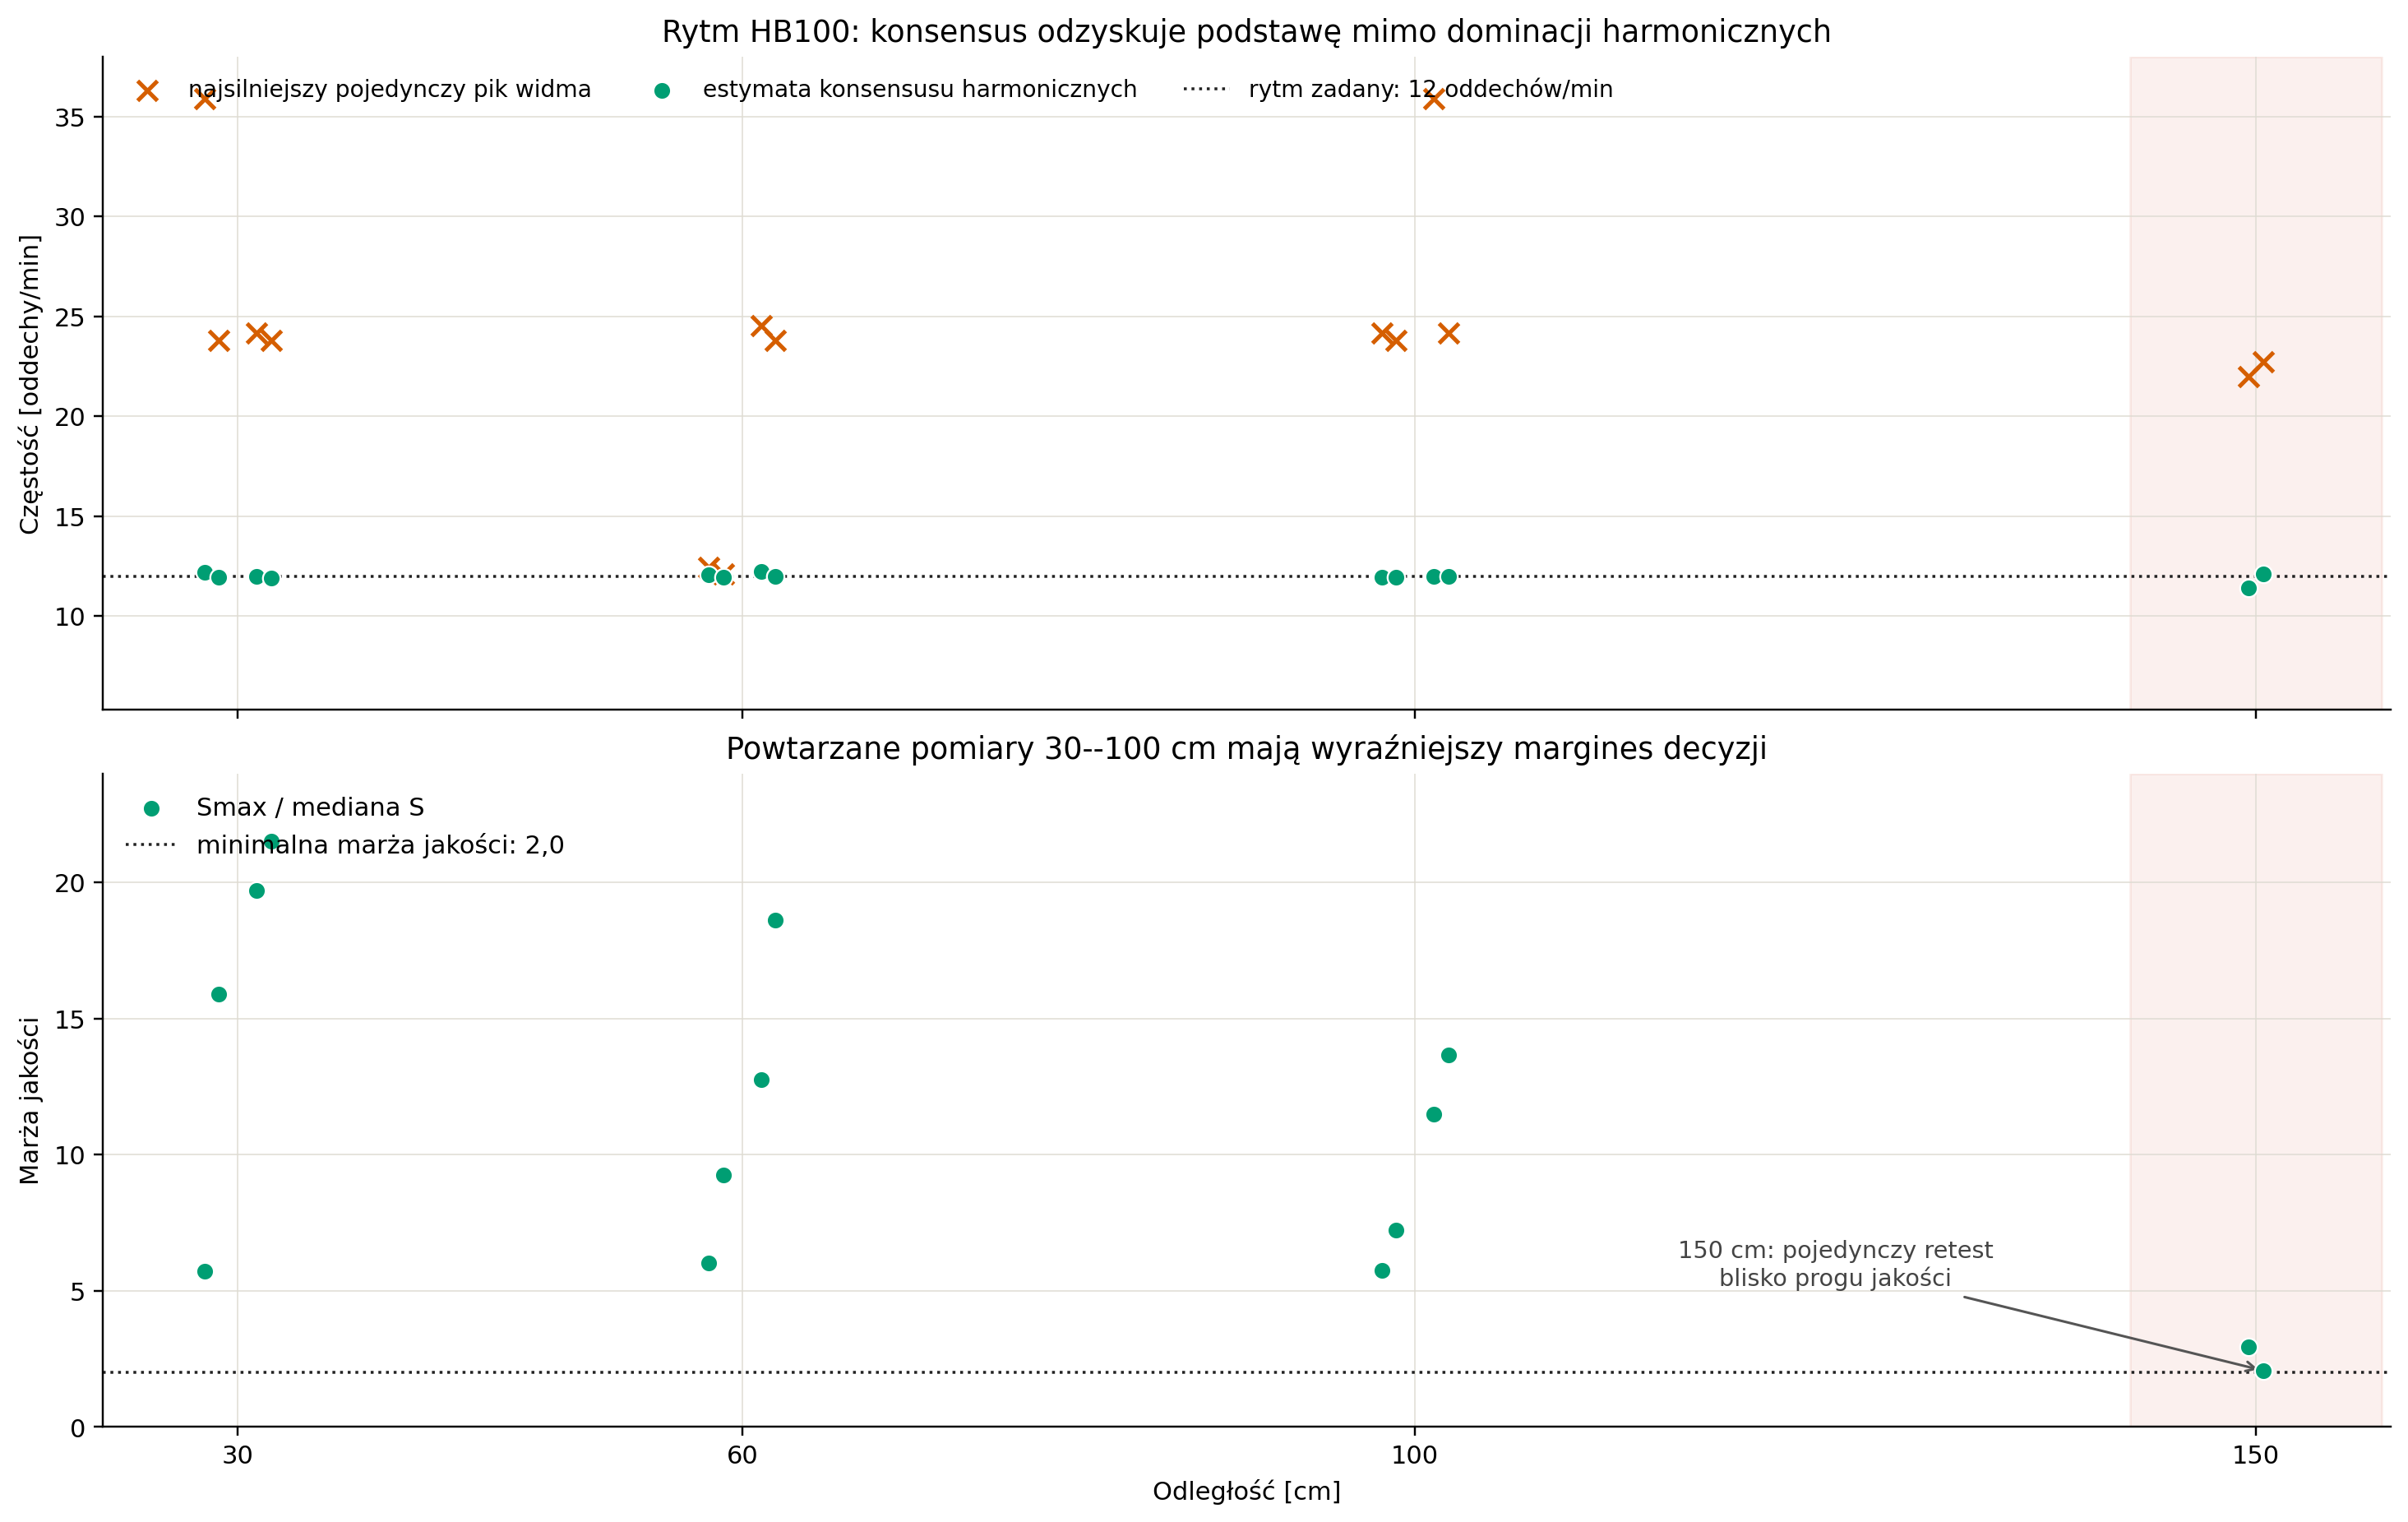
\includegraphics[width=\textwidth]{hb100_a121_rytm_dystanse.png}
    \caption[Profile konsensusu HB100 i rytm A121 dla 30--150 cm]{Porównanie
    estymacji rytmu we wszystkich 14 blokach. Górny rząd przedstawia funkcję
    konsensusu harmonicznych $S(f)$ dla HB100: jasne linie są profilami
    pojedynczych bloków, ciemna --- ich medianą dla danego dystansu. Linia
    kropkowana wyznacza zadane 12~oddechów/min, zielona --- medianę estymat
    HB100, a~niebieskie trójkąty --- pik \SIrange{0.10}{0.30}{Hz} z~A121.
    Dolny panel pokazuje wynik każdego bloku; krzyżyki to mylące najsilniejsze
    piki HB100 przed złożeniem harmonicznych. Przy \SIrange{30}{100}{cm}
    profile HB100 mają wyraźniejszą przewagę kandydata przy 12~oddechach/min
    ($S_{\max}/\operatorname{med}S=5{,}7$--$21{,}5$) niż w~pojedynczym
    reteście \SI{150}{cm} (2,1--2,9).}
    \label{fig:hb100-a121-rytm-dystanse}
\end{figure}

\begin{figure}[H]
    \centering
    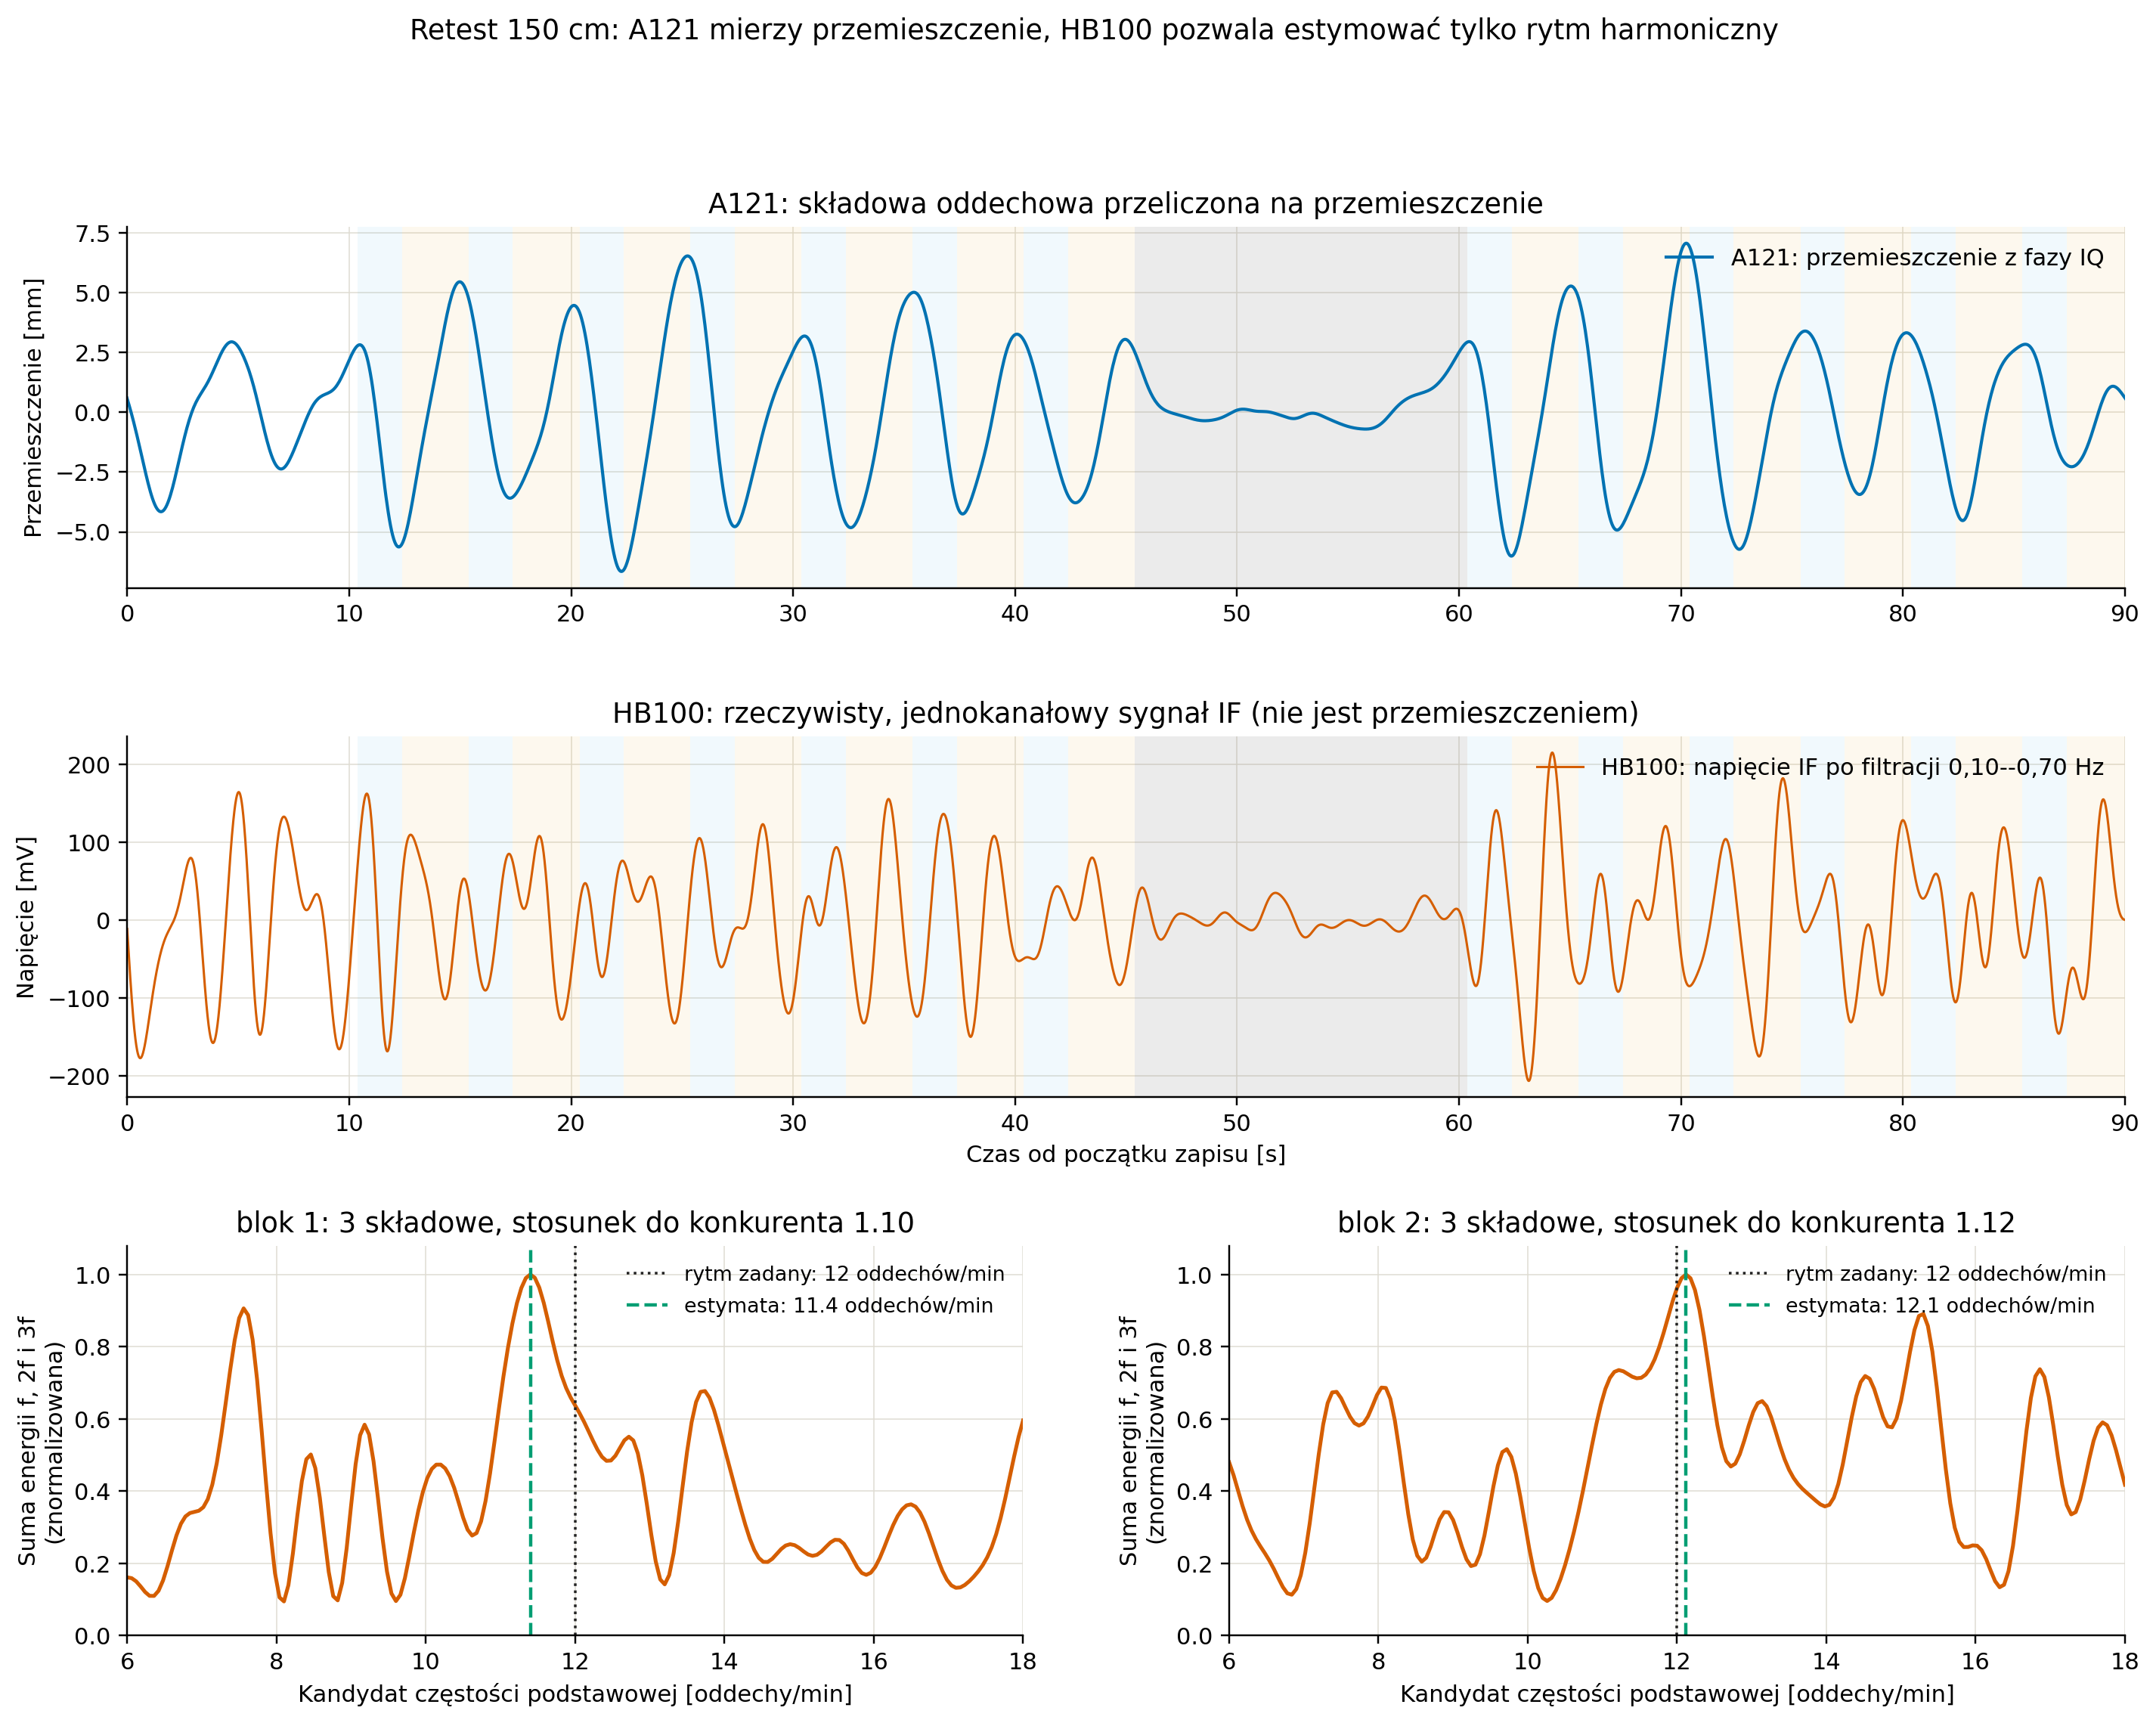
\includegraphics[width=\textwidth]{hb100_a121_150cm_retest.png}
    \caption[Oddzielny retest HB100 i A121 na 150 cm]{Pojedynczy retest na
    \SI{150}{cm}, wyodrębniony z~powtarzanej serii ze względu na brak
    powtórzenia. Górny panel pokazuje przemieszczenie wyznaczone z~fazy IQ
    A121, środkowy --- jednokanałowe napięcie IF HB100; zachowano osobne
    jednostki, aby nie sugerować ich równoważności. Dolne panele pokazują
    funkcję~\eqref{eq:hb100-harmonic-consensus}: mimo najsilniejszych pików
    napięcia przy około \SI{0.37}{Hz}, estymator wskazał \SI{0.190}{Hz}
    (11,4~oddechów/min) oraz \SI{0.202}{Hz} (12,1~oddechów/min) wobec
    zadanego rytmu \SI{0.20}{Hz}. Marże jakości 2,9 i~2,1 są jednak blisko
    progu akceptacji 2,0; pojedynczy retest stanowi więc jedynie graniczne
    wskazanie rytmu, a~nie podstawę do estymacji fazy wdech--wydech.}
    \label{fig:hb100-a121-150cm}
\end{figure}

\begin{figure}[H]
    \centering
    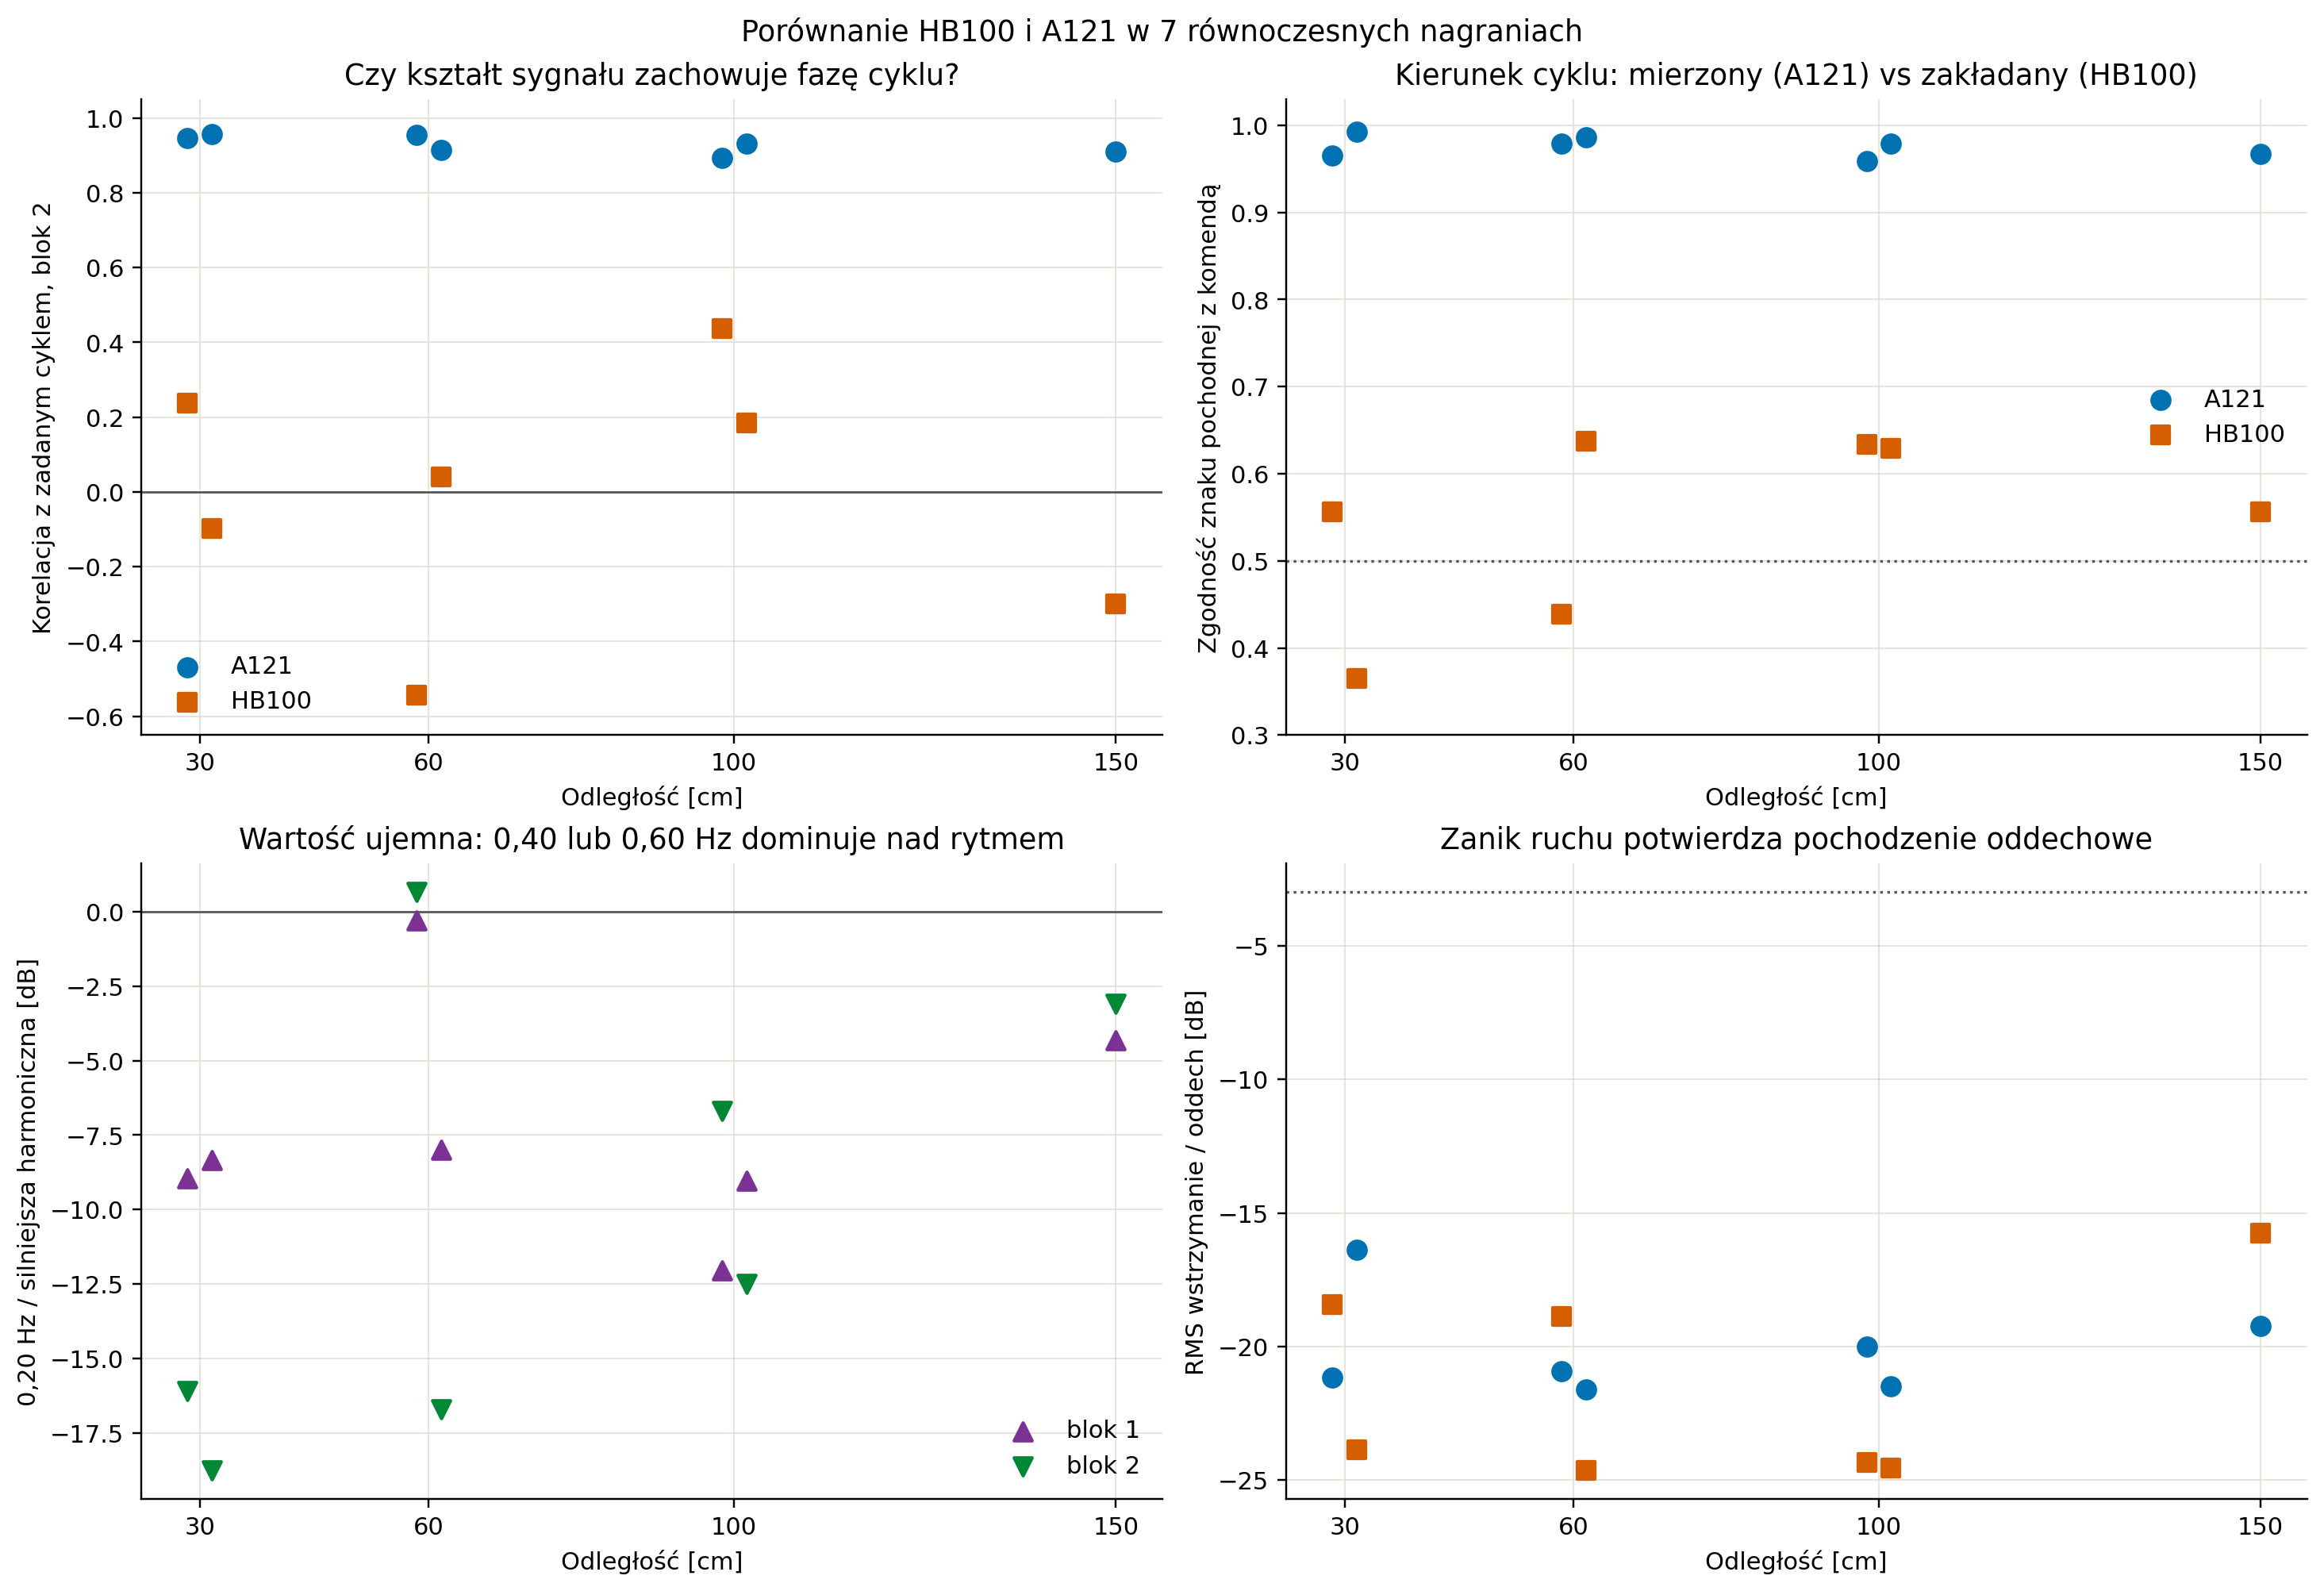
\includegraphics[width=\textwidth]{hb100_a121_metryki.png}
    \caption[Metryki porównania HB100 i A121]{Metryki sześciu prób podstawowych
    oraz pojedynczego retestu \SI{150}{cm}. Dwa górne
    panele dotyczą drugiego bloku po kalibracji polaryzacji na pierwszym.
    Prawy górny panel przedstawia zgodność znaku pochodnej sygnału
    z~komendą. Dla A121 jest to rzeczywisty kierunek ruchu klatki, ponieważ
    faza IQ niesie znak przemieszczenia. Dla HB100 jest to test naiwnego
    założenia, że rzeczywiste napięcie IF zachowuje się jak przemieszczenie;
    równanie~\eqref{eq:hb100-pochodna-if} przewiduje niepowodzenie tego
    założenia, a~panel to przewidywanie weryfikuje. Wartości HB100 nie skupiają
    się wokół 50\%, lecz układają po obu stronach tej linii --- to sygnatura
    znaku narzuconego przez fazę statyczną, nie szumu. Lewy dolny panel pokazuje
    poziom składowej \SI{0.20}{Hz} względem
    silniejszej z~harmonicznych \SI{0.40}{Hz} i~\SI{0.60}{Hz}; wartość ujemna
    oznacza dominację harmonicznej. Prawy dolny panel przedstawia zanik RMS
    podczas wstrzymania; linia kropkowana wskazuje próg $-3$~dB. Przesunięcie
    punktów wokół dystansu rozróżnia dwa powtórzenia.}
    \label{fig:hb100-a121-metryki}
\end{figure}

\section{Wnioski i zakres zastosowania HB100}

\paragraph{HB100 wykrywał aktywność oddechową.} W~sześciu próbach serii podstawowej
RMS pasma HB100 malał podczas wstrzymania o~\SIrange{18.4}{24.6}{dB}. Na
\SI{100}{cm} RMS w~odcinkach sterowanych wynosił \SI{132.3}{mV} i~
\SI{179.8}{mV}, czyli odpowiednio o~\SI{27.4}{dB} i~\SI{30.1}{dB} więcej niż
\SI{5.615}{mV} tła z~pustej sceny. Tor miał więc wyraźny zapas do wykrywania
ruchu oddechowego na największym zbadanym dystansie. Przy \SI{30}{cm}
odpowiednio 1,55\% i~4,33\% próbek przekraczało przyjęty próg nasycenia;
przy \SI{60}{cm} i~\SI{100}{cm} nasycenie nie wystąpiło. Obecne wzmocnienie
jest zatem zbyt duże do wiernej rejestracji głębokiego oddechu z~bardzo małej
odległości.

\paragraph{Retest graniczny \SI{150}{cm}.} W~pojedynczej próbie na
\SI{150}{cm} oba tory nadal reagowały na zatrzymanie ruchu: RMS HB100 podczas
wstrzymania był o~\SI{15.7}{dB} niższy niż w~odcinkach sterowanych. Sygnał
HB100 nie zachował kierunku fazy: w~dwóch blokach dominowały surowe piki
odpowiednio \SI{0.366}{Hz} i~\SI{0.378}{Hz}, korelacja z~komendami po
jednorazowej kalibracji znaku wyniosła $-0{,}299$, a~zgodność znaku pochodnej
z~komendą 36,6\%, czyli była systematycznie odwrócona. Jednocześnie konsensus harmoniczny wskazał
\SI{0.190}{Hz} i~\SI{0.202}{Hz}, czyli rytm bliski zadanym \SI{0.20}{Hz}
(rys.~\ref{fig:hb100-a121-150cm}). Marże jakości 2,9 i~2,1 były jednak
zaledwie na poziomie progu akceptacji 2,0 i~wyraźnie słabsze niż w~powtarzanej
serii \SIrange{30}{100}{cm}. Na \SI{150}{cm} można więc mówić co najwyżej
o~granicznym wskazaniu rytmu, a~nie o~powtarzalnej estymacji częstości.
Estymacja faz wdech--wydech nie jest w~tej geometrii użyteczna. W~tym samym
nagraniu A121 z~płaską pokrywą osiągnął $r=0{,}910$ i~96,7\% zgodności
kierunku. Jest to jednak tylko jeden retest; nie wyznacza ogólnego zasięgu
żadnego z~radarów, a~zwłaszcza A121 z~soczewką skupiającą.

\paragraph{Dominują harmoniczne, a~nie zadany rytm.} W~serii podstawowej w~10 z~12 sterowanych
bloków najwyższy pik HB100 w~paśmie \SIrange{0.10}{0.65}{Hz} leżał przy
około \SI{0.40}{Hz} albo \SI{0.60}{Hz}, mimo że klatka wykonywała cykle
\SI{0.20}{Hz}. Tylko oba bloki pierwszej próby na \SI{60}{cm} miały maksimum
blisko częstości podstawowej. Jest to zgodne z~modelem
\eqref{eq:cw-baseband}: pojedynczy kanał obserwuje cosinus fazy, więc przy
niekorzystnym punkcie pracy jeden cykl przemieszczenia może utworzyć dwa
ekstrema napięcia. Efekt dodatkowo wzmacnia charakterystyka analogowa. Z~modelu
\eqref{eq:hb100-transfer} wynika wzmocnienie $45{,}6\times$ przy
\SI{0.20}{Hz}, $90{,}3\times$ przy \SI{0.40}{Hz} i~$105{,}7\times$ przy
\SI{0.60}{Hz}; druga i~trzecia harmoniczna otrzymują więc odpowiednio około
5,9 i~7,3~dB przewagi względem składowej podstawowej jeszcze przed ADC.
Obcinanie amplitudy (ang. \emph{clipping}) w~próbach \SI{30}{cm} wytwarza
kolejne harmoniczne. Najsilniejszy pik widma nie jest zatem dobrym estymatorem
częstości, ale sam układ pików pozostaje użyteczny dla
funkcji~\eqref{eq:hb100-harmonic-consensus}.

\paragraph{Brak kierunku wdech--wydech w~HB100 potwierdza model, a~nie
niedoskonałość wykonania.} Dla A121 korelacja drugiego bloku z~komendami
wynosiła 0,894--0,957, a~zgodność kierunku 95,9--99,3\%. Dla HB100 wartości
wynosiły odpowiednio od $-0{,}543$ do 0,438 oraz 36,5--63,7\%. Jest to
dokładnie to, czego wymaga równanie~\eqref{eq:hb100-pochodna-if}: przy
nieznanym czynniku $-\sin(\cdot)$ zależnym od fazy statycznej celu żaden dobór
polaryzacji nie może ustalić kierunku.

Rozkład tych wartości jest przy tym bardziej wymowny niż sama ich wielkość.
Nie są to wyniki „bliskie losowym'': 36,5\% i~36,6\% oznaczają
\emph{systematyczne odwrócenie} kierunku, a~nie brak informacji. Gdyby sygnał
był szumem, $Q_H$ skupiłoby się wokół 50\%; tymczasem rozrzut 36--64\% układa
się po obu stronach tej wartości, co jest sygnaturą znaku ustalanego osobno
przez punkt pracy każdego nagrania. W~jednej próbie na \SI{60}{cm} relacja
była umiarkowanie dodatnia w~pierwszym bloku, a~po wstrzymaniu stała się
wyraźnie ujemna mimo niezmienionej polaryzacji --- czyli mapowanie odwróciło
się w~obrębie jednego nagrania. Informacja o~ruchu jest zatem w~napięciu
obecna, lecz jej znak jest przypisywany przez geometrię, a~nie przez fazę
oddechu. Właśnie dlatego użyteczny okazał się estymator, który znaku w~ogóle
nie używa, opierając się wyłącznie na energii harmonicznych
(równanie~\eqref{eq:hb100-harmonic-consensus}).

Łącznie wyniki rozdzielają trzy poziomy użyteczności: wykrycie ruchu
oddechowego, oszacowanie jego okresowości oraz rozpoznanie kierunku fazy.
HB100 wiarygodnie realizował pierwszy z~nich. Dla długich bloków pełnego,
sterowanego oddechu na \SIrange{30}{100}{cm} estymator konsensusu
harmonicznych pozwolił warunkowo wyznaczyć rytm, łącząc kandydatów $f$, $2f$
i~$3f$. Jest to najwyższy poziom interpretacji, jaki dane uzasadniają dla
HB100: pomocniczy wskaźnik rytmu po przejściu rygorystycznej kontroli jakości.
Przy \SI{150}{cm} nawet ta interpretacja pozostaje graniczna, a~kierunku
wdech--wydech nie udało się zachować po jednorazowej kalibracji znaku.

Najbardziej uzasadnionym zastosowaniem HB100 jest więc tania detekcja ruchu
lub obecności aktywności oddechowej w~stałej scenie z~jedną osobą. Nie jest to
jednoznaczna detekcja człowieka: brak sygnału może oznaczać nieobecność,
wstrzymanie oddechu, minimum fazowe, zmianę pozycji albo złe skierowanie.
HB100 nie powinien zatem samodzielnie rozstrzygać o~bezdechu ani fazie cyklu.
Do analizy wdech--wydech i~przemieszczenia klatki właściwszy pozostaje A121,
który udostępnia bramki odległościowe i~zespolony sygnał I/Q. Wniosek ten jest
zgodny z~literaturą: przewagę toru kwadraturowego nad odbiornikiem
jednokanałowym w~pomiarze parametrów krążeniowo-oddechowych wykazano
ilościowo już w~\cite{droitcour2004}, a~demodulacja arcus tangens z~pary I/Q
pozostaje standardowym sposobem obejścia punktów zerowych \cite{park2007}.
Przedstawiony pomiar dodaje do tego obrazu rozróżnienie trzech poziomów
użyteczności oraz pokazuje, że rytm --- w~przeciwieństwie do kierunku fazy ---
bywa odzyskiwalny nawet z~jednego kanału rzeczywistego. Estymator HB100
może służyć jedynie jako ostrożny wskaźnik rytmu w~stabilnym, wystarczająco
silnym fragmencie ruchu na krótkim dystansie, z~jawnym odrzuceniem wyniku
niejednoznacznego. Nie jest porównywalny z~A121 jako źródło informacji
o~fazie oddechu, ponieważ A121 zachował zgodność kierunku bliską 96--99\%
w~powtarzanej serii.

% =====================================================================
\chapter{Eksperyment: soczewki dielektryczne i wzmacnianie odbicia}
\label{chap:soczewki}

\section{Cel i hipotezy}
Celem eksperymentu było sprawdzenie dwóch hipotez:
\begin{enumerate}
  \item wybór soczewki dielektrycznej istotnie wpływa na jakość sygnału
  oddechowego rejestrowanego przez radar A121,
  \item naklejenie na klatkę piersiową łaty z~folii aluminiowej
  (\SI{5}{cm}~$\times$~\SI{5}{cm}) wzmacnia odbicie i~poprawia jakość
  sygnału.
\end{enumerate}
Druga hipoteza jest o~tyle istotna, że sama amplituda odbicia nie jest
wystarczającym kryterium --- silniejsze odbicie może współwystępować
z~gorszym stosunkiem sygnału oddechowego do szumu.

Jak opisano w~sekcji~\ref{sec:materialy-radar}, folia jest dla fal
\SI{60}{GHz} praktycznie nieprzezroczystym przewodnikiem i~silnym reflektorem.
Nie wynika z~tego jednak, że niewielka łata poprawi pomiar człowieka. Radar już
otrzymuje rozłożone przestrzennie odbicie od bogatych w~wodę tkanek, a~dodanie
metalowej powierzchni może zmienić dominującą bramkę, fazę i~tory wielodrogowe.
Hipotezę należy więc sprawdzać na podstawie SNR i~powtarzalności estymacji,
a~nie na podstawie samej przewodności aluminium.

\section{Badane soczewki}
Porównano trzy warianty przesłony czujnika (rys.~\ref{fig:soczewki}):
soczewkę hiperboliczną (refrakcyjną), soczewkę FZP (dyfrakcyjną płytkę
strefową Fresnela) oraz płaską pokrywę bez własności skupiających.

\begin{figure}[p]
    \centering
    \begin{subfigure}{0.72\textwidth}
        \centering
        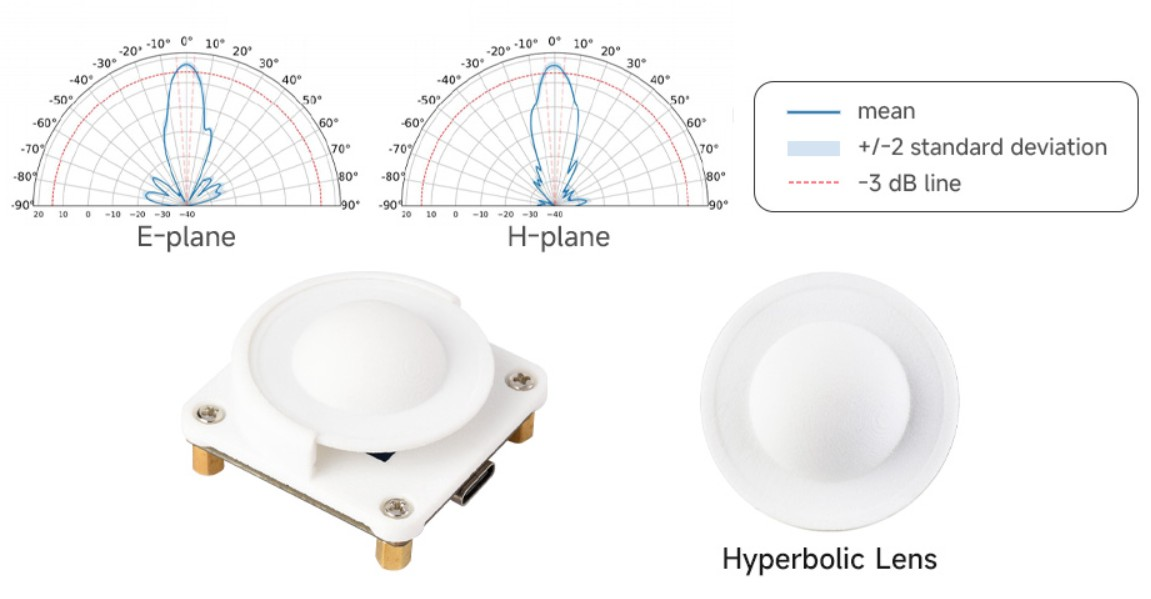
\includegraphics[width=\textwidth]{soczewka_hiperboliczna.jpg}
        \caption{Soczewka hiperboliczna --- wąska wiązka igłowa, niskie
        listki boczne.}
    \end{subfigure}
    \\[0.8em]
    \begin{subfigure}{0.72\textwidth}
        \centering
        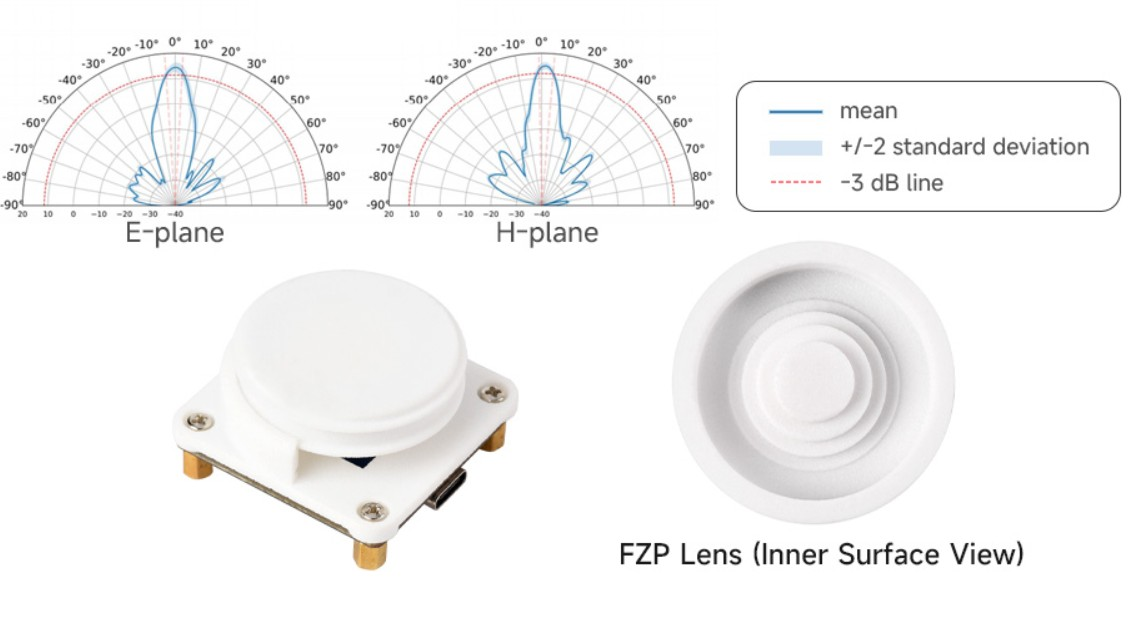
\includegraphics[width=\textwidth]{soczewka_fzp.jpg}
        \caption{Soczewka FZP --- porównywalny zysk, wyraźnie silniejsze
        listki boczne.}
    \end{subfigure}
    \\[0.8em]
    \begin{subfigure}{0.72\textwidth}
        \centering
        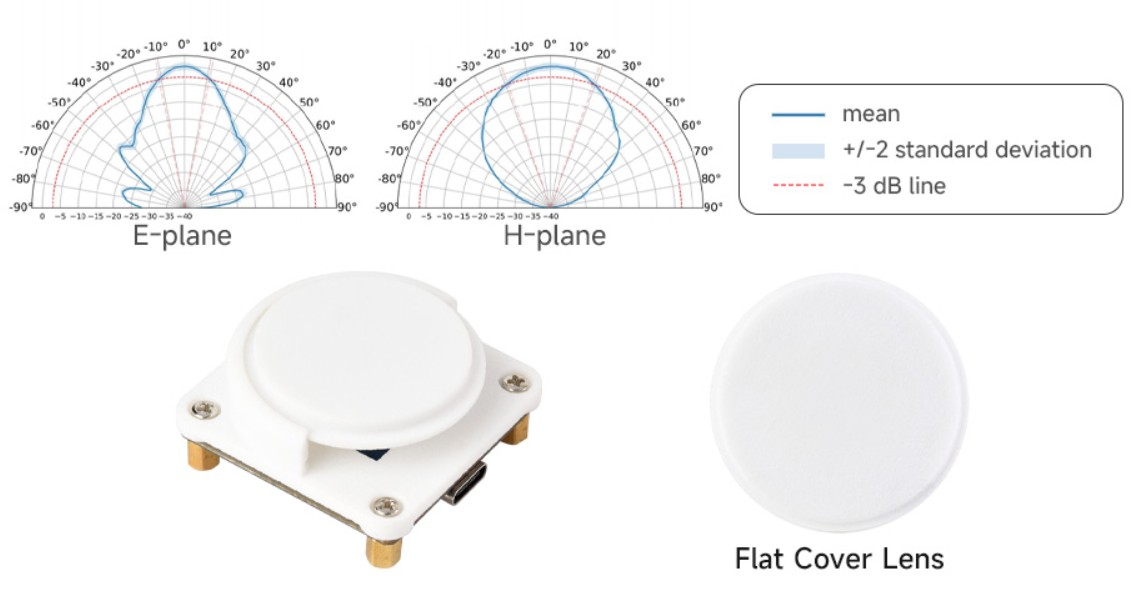
\includegraphics[width=\textwidth]{soczewka_flat_cover.jpg}
        \caption{Płaska pokrywa --- brak skupiania, szeroka wiązka.}
    \end{subfigure}
    \caption[Charakterystyki promieniowania badanych soczewek]{Badane
    warianty przesłony czujnika A121 wraz z~charakterystykami promieniowania
    w~płaszczyznach E i~H (materiały producenta \cite{waveshare_a121}).}
    \label{fig:soczewki}
\end{figure}

\section{Metodyka}
Zrealizowano plan pełny: 3~soczewki $\times$ 2~odległości
(\SI{50}{cm} i~\SI{100}{cm}) $\times$ 2~stany folii (naklejona / brak)
$=$ 12~warunków, każdy powtórzony trzykrotnie, co dało \textbf{36~nagrań}
po \SI{60}{s} (około 1200 ramek każde). Akwizycję prowadzono sterowaną
procedurą (\texttt{tools/a121\_guided\_experiment.py}), która prowadzi
operatora przez kolejne warunki. W~każdym nagraniu badany oddychał swobodnie,
bez narzuconej częstości i~bez komend oznaczających granice wdechu oraz
wydechu. Celem tej serii było porównanie przesłon i~folii, a~nie walidacja faz
pojedynczego cyklu; analizowano więc rytm występujący naturalnie w~danym
nagraniu.

Radar był zamocowany na fotograficznym statywie Manfrotto. Odległości
\SI{50}{cm} i~\SI{100}{cm} ustawiano za pomocą dalmierza laserowego
MILESEEY~D2 w~wariancie \SI{40}{m}; producent deklaruje dla rodziny D2
dokładność pomiaru odległości $\pm\SI{2}{mm}$ \cite{mileseey_d2}. Plamkę
lasera wykorzystywano również do orientacyjnej kontroli kierunku osi
stanowiska, tak aby wypadała na centralnym obszarze klatki piersiowej.
W~obrębie danej serii nie zmieniano wysokości ani nachylenia statywu.

\begin{figure}[H]
    \centering
    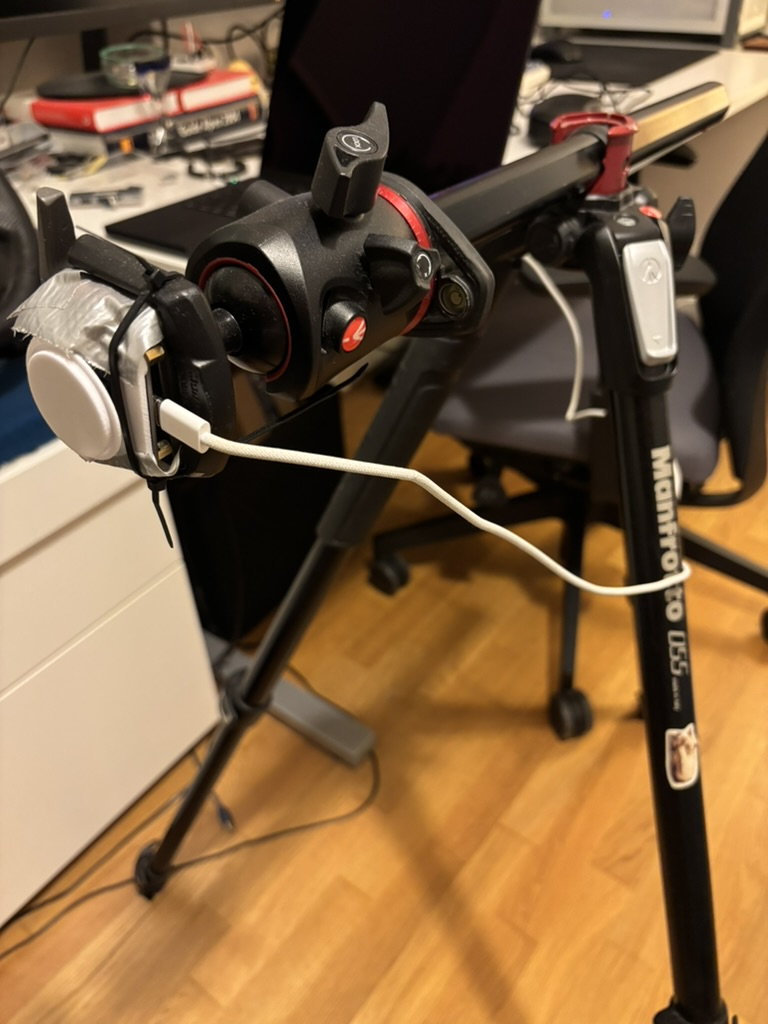
\includegraphics[width=0.52\textwidth]{stanowisko_a121_mocowanie.jpg}
    \caption[Mocowanie radaru A121 na statywie]{Moduł A121 w~wymiennej
    przesłonie zamocowany do głowicy fotograficznego statywu Manfrotto.
    Głowica umożliwiała zablokowanie kierunku osi, a~to samo mocowanie
    wykorzystywano w~serii przy \SI{50}{cm} i~\SI{100}{cm}. Na zdjęciu
    widoczna jest płaska pokrywa; w~pozostałych warunkach wymieniano wyłącznie
    przedni element optyczny.}
    \label{fig:mocowanie-a121}
\end{figure}

Badany siedział na krześle w~naturalnej, niewymuszonej pozycji. Oś radaru
utrzymywano równolegle do podłoża, co kontrolowano poziomnicą pęcherzykową
wbudowaną w~dalmierz. Ze względu na naturalne pochylenie tułowia oś radaru
była odchylona o~około \SI{30}{\degree} od normalnej do powierzchni klatki
piersiowej, czyli kąt padania wynosił w~przybliżeniu \SI{30}{\degree}. W~serii
z~folią stosowano kwadrat o~wymiarach $\SI{5}{cm}\times\SI{5}{cm}$, umieszczony
tak, aby jego górna krawędź znajdowała się \SI{5}{cm} poniżej poziomej linii
łączącej brodawki sutkowe.

Dla każdego nagrania wyznaczono: amplitudę odbicia w~bramkach klatki
piersiowej, stosunek sygnału oddechowego do szumu (SNR --- maksimum widma
w~paśmie \SIrange{0.08}{0.60}{Hz} względem mediany tła
\SIrange{1}{5}{Hz}), wyrazistość piku widmowego, stabilność śledzonej
odległości celu, amplitudę przemieszczenia oddechowego oraz poziom szumu
ruchowego w~paśmie \SIrange{4}{8}{Hz}.

\paragraph{Ograniczenie metodyczne.} Kolejność pomiarów nie była
randomizowana --- wszystkie nagrania z~folią wykonano przed wszystkimi
nagraniami bez folii, w~dwóch oddzielnych, kolejnych sesjach.
Efekt folii jest więc splątany z~efektem sesji (postawa, ustawienie czujnika,
stan badanego). Porównania między soczewkami są natomiast zrównoważone
względem sesji i~pozostają wiarygodne.

\section{Wyniki: porównanie soczewek}

\begin{figure}[H]
    \centering
    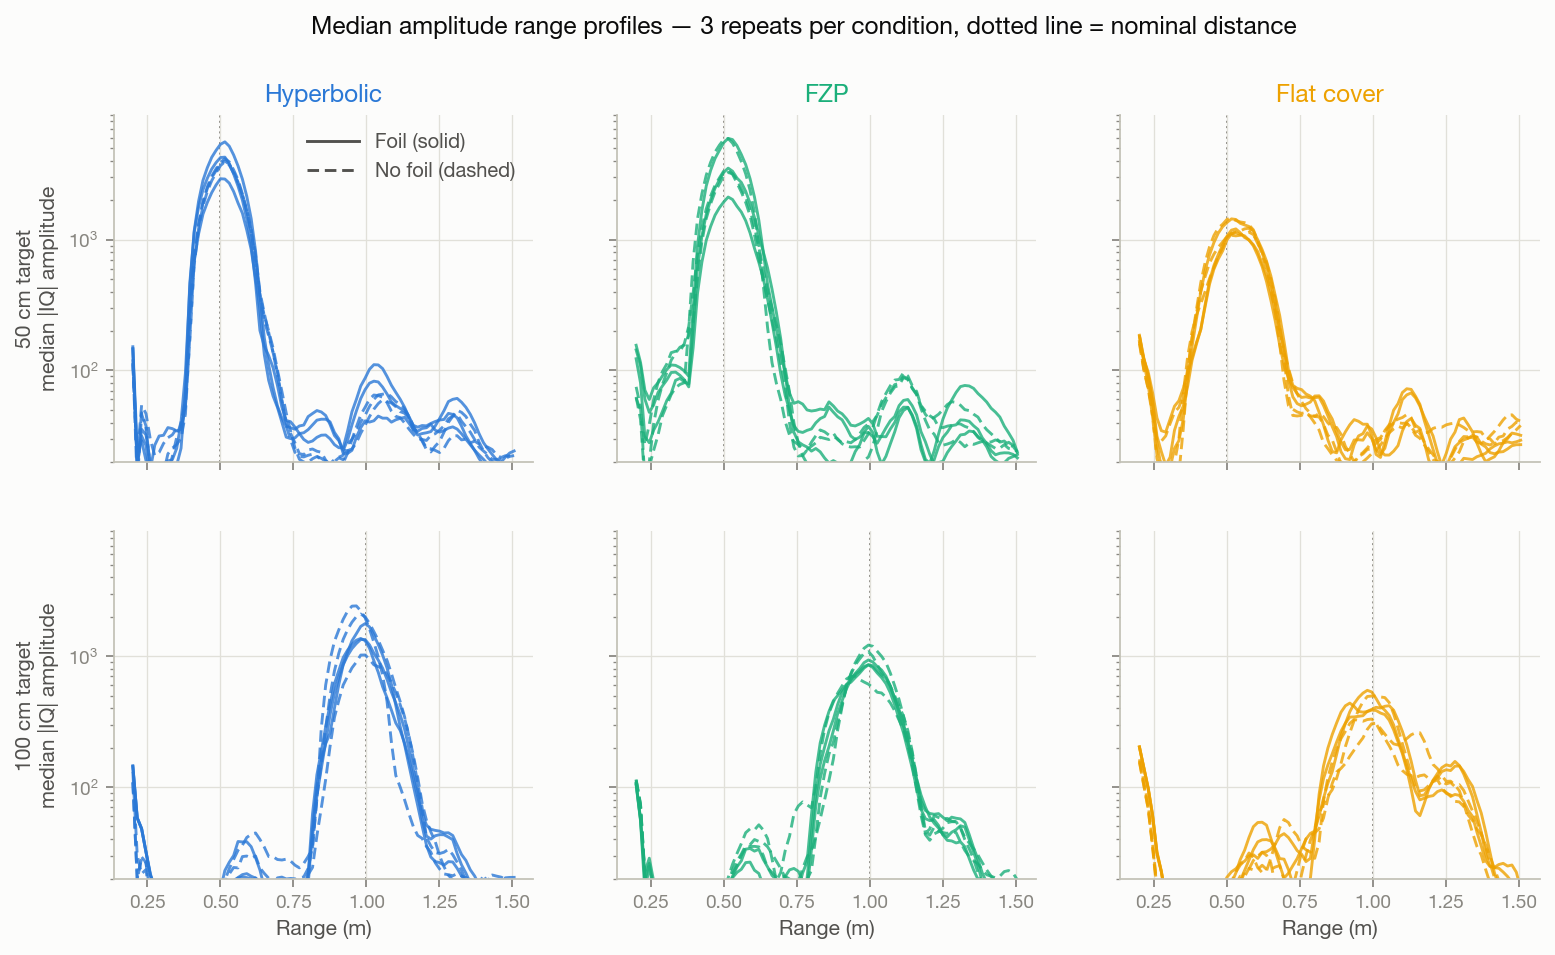
\includegraphics[width=\textwidth]{foil_profile_zasiegu.png}
    \caption[Profile amplitudy w funkcji odległości]{Medianowa amplituda
    sygnału w~funkcji odległości dla wszystkich 36~nagrań. Kolumny odpowiadają
    soczewkom, a~wiersze odległościom \SI{50}{cm} i~\SI{100}{cm}. Każda cienka
    krzywa jest medianą po czasie z~jednego nagrania (po trzy powtórzenia);
    linia ciągła oznacza folię, przerywana jej brak, a~pionowa kropkowana ---
    odległość nominalną. Logarytmiczna oś pionowa pokazuje jednocześnie pik
    klatki i~słabsze odbicia tła. Soczewki skupiające dają 3--10-krotnie
    wyższy pik; przy \SI{100}{cm} pik płaskiej pokrywy jest szeroki i~słabo
    oddzielony od sąsiednich bramek.}
    \label{fig:profile}
\end{figure}

Na rysunku~\ref{fig:profile} nie należy porównywać wyłącznie wysokości
najwyższego punktu. Wąski, powtarzalny pik oznacza, że energia wraca z~tego
samego fragmentu tułowia, natomiast szeroki profil może obejmować kilka
części ciała i~tło. To wyjaśnia, dlaczego płaska pokrywa przy \SI{100}{cm}
może nadal rejestrować oddech, a~zarazem niestabilnie wybierać bramkę celu.

\begin{table}[H]
\centering
\caption{Uśrednione metryki dla każdej soczewki i~odległości (n=6: oba stany
folii $\times$ 3~powtórzenia).}
\label{tab:soczewki}
\small
\begin{tabular}{@{}llrrrr@{}}
\toprule
Odległość & Soczewka & Amplituda & SNR & Odch. std. & Przemieszcz. \\
 & & [j.u.] & [dB] & odl. [cm] & [mm] \\
\midrule
\SI{50}{cm}  & Hiperboliczna & 3100 & 45,3 & 1,0 & 2,20 \\
             & FZP           & 3020 & 46,6 & 1,2 & 2,45 \\
             & Płaska pokrywa & 970 & 43,8 & 3,5 & 1,56 \\
\midrule
\SI{100}{cm} & Hiperboliczna & 1245 & 45,7 & 2,4 & 2,23 \\
             & FZP           &  697 & 47,3 & 3,7 & 2,10 \\
             & Płaska pokrywa & 322 & 45,9 & 8,9 & 1,79 \\
\bottomrule
\end{tabular}
\end{table}

Wyniki prowadzą do trzech obserwacji:

\paragraph{Amplituda.} Przy \SI{50}{cm} obie soczewki skupiające są
równoważne (mediana ok. 3000~j.u.) i~około trzykrotnie lepsze od płaskiej
pokrywy. Przy \SI{100}{cm} soczewka hiperboliczna wyraźnie wygrywa ---
zachowuje 40\% amplitudy z~\SI{50}{cm}, podczas gdy FZP tylko 23\%, co daje
jej około 1,8-krotną przewagę. Jest to spójne z~naturą soczewki FZP, której
ogniskowanie jest zoptymalizowane dla konkretnej odległości ogniskowej,
podczas gdy soczewka hiperboliczna kolimuje wiązkę.

\paragraph{Stabilność śledzenia celu.} Metryka ta różnicuje soczewki
najsilniej. Odchylenie standardowe śledzonej odległości piku rośnie od
\SI{1.0}{cm} (hiperboliczna, \SI{50}{cm}) do \SI{8.9}{cm} (płaska pokrywa,
\SI{100}{cm}). Przy metrze odległości płaska pokrywa utrzymuje cel
w~dominującej bramce jedynie w~14--54\% ramek --- szeroka wiązka oświetla
jednocześnie tors, ramiona i~tło, przez co „najsilniejszy odbłysk” przeskakuje
między obiektami. Logarytm amplitudy niemal idealnie przewiduje stabilność
śledzenia ($\rho_{\mathrm{Spearman}} = -0{,}93$).

\paragraph{SNR oddechowy --- brak różnic.} Najistotniejszy wynik: stosunek
sygnału oddechowego do szumu wynosi 44--47~dB \emph{niezależnie} od soczewki,
a~amplituda w~ogóle go nie przewiduje ($\rho = 0{,}08$; $p = 0{,}64$). Żadna
z~par soczewek nie różni się istotnie statystycznie. Przy zapasie SNR rzędu
40~dB dziesięciokrotna przewaga amplitudy nie przekłada się na wykrywalność
oddechu.

\begin{figure}[H]
    \centering
    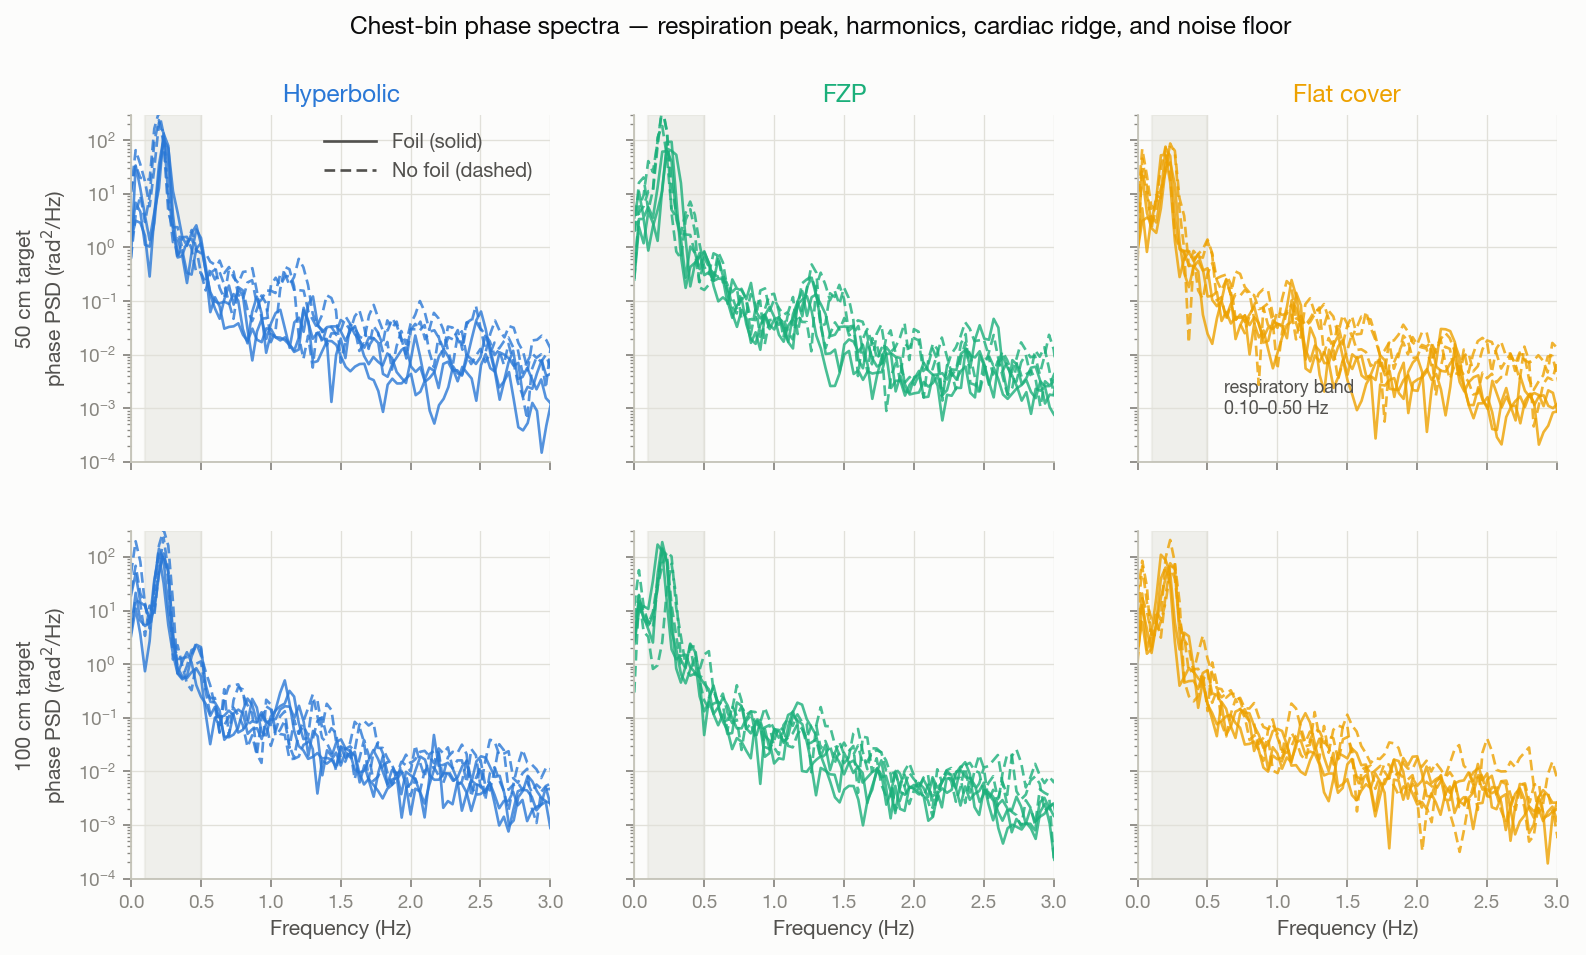
\includegraphics[width=\textwidth]{foil_widma_fazy.png}
    \caption[Widma sygnału fazowego]{Widma gęstości mocy sygnału fazowego
    z~bramek klatki piersiowej; układ paneli i~rodzaje linii są takie jak na
    rys.~\ref{fig:profile}, a~każda krzywa odpowiada jednemu nagraniu.
    Zacieniono pasmo oddechowe \SIrange{0.10}{0.50}{Hz}; jego główny pik leży
    zwykle w~okolicy \SIrange{0.20}{0.27}{Hz}, a~słabszy składnik w~pobliżu
    dwukrotności tej częstotliwości jest harmoniczną niesinusoidalnego ruchu
    klatki. Oś mocy jest logarytmiczna. Wybór soczewki niemal nie zmienia
    odległości piku od lokalnego tła widmowego.}
    \label{fig:widma}
\end{figure}

Wysokość krzywej na rys.~\ref{fig:widma} opisuje zmienność \emph{fazy}, a~nie
bezpośrednio moc odbitego echa z~rys.~\ref{fig:profile}. Dlatego słabsza
amplituda IQ może współistnieć z~wyraźnym pikiem oddechu. Składowych w~okolicy
\SIrange{1}{1.5}{Hz} nie interpretowano jako pewnego tętna bez niezależnego
wzorca; mogą zawierać zarówno mikroruch sercowy, jak i~harmoniczne oraz ruch.
Wykres kończy się przy \SI{3}{Hz}, natomiast mianownik raportowanego SNR
wyznaczano osobno z~pasma \SIrange{4}{8}{Hz}.

\begin{figure}[H]
    \centering
    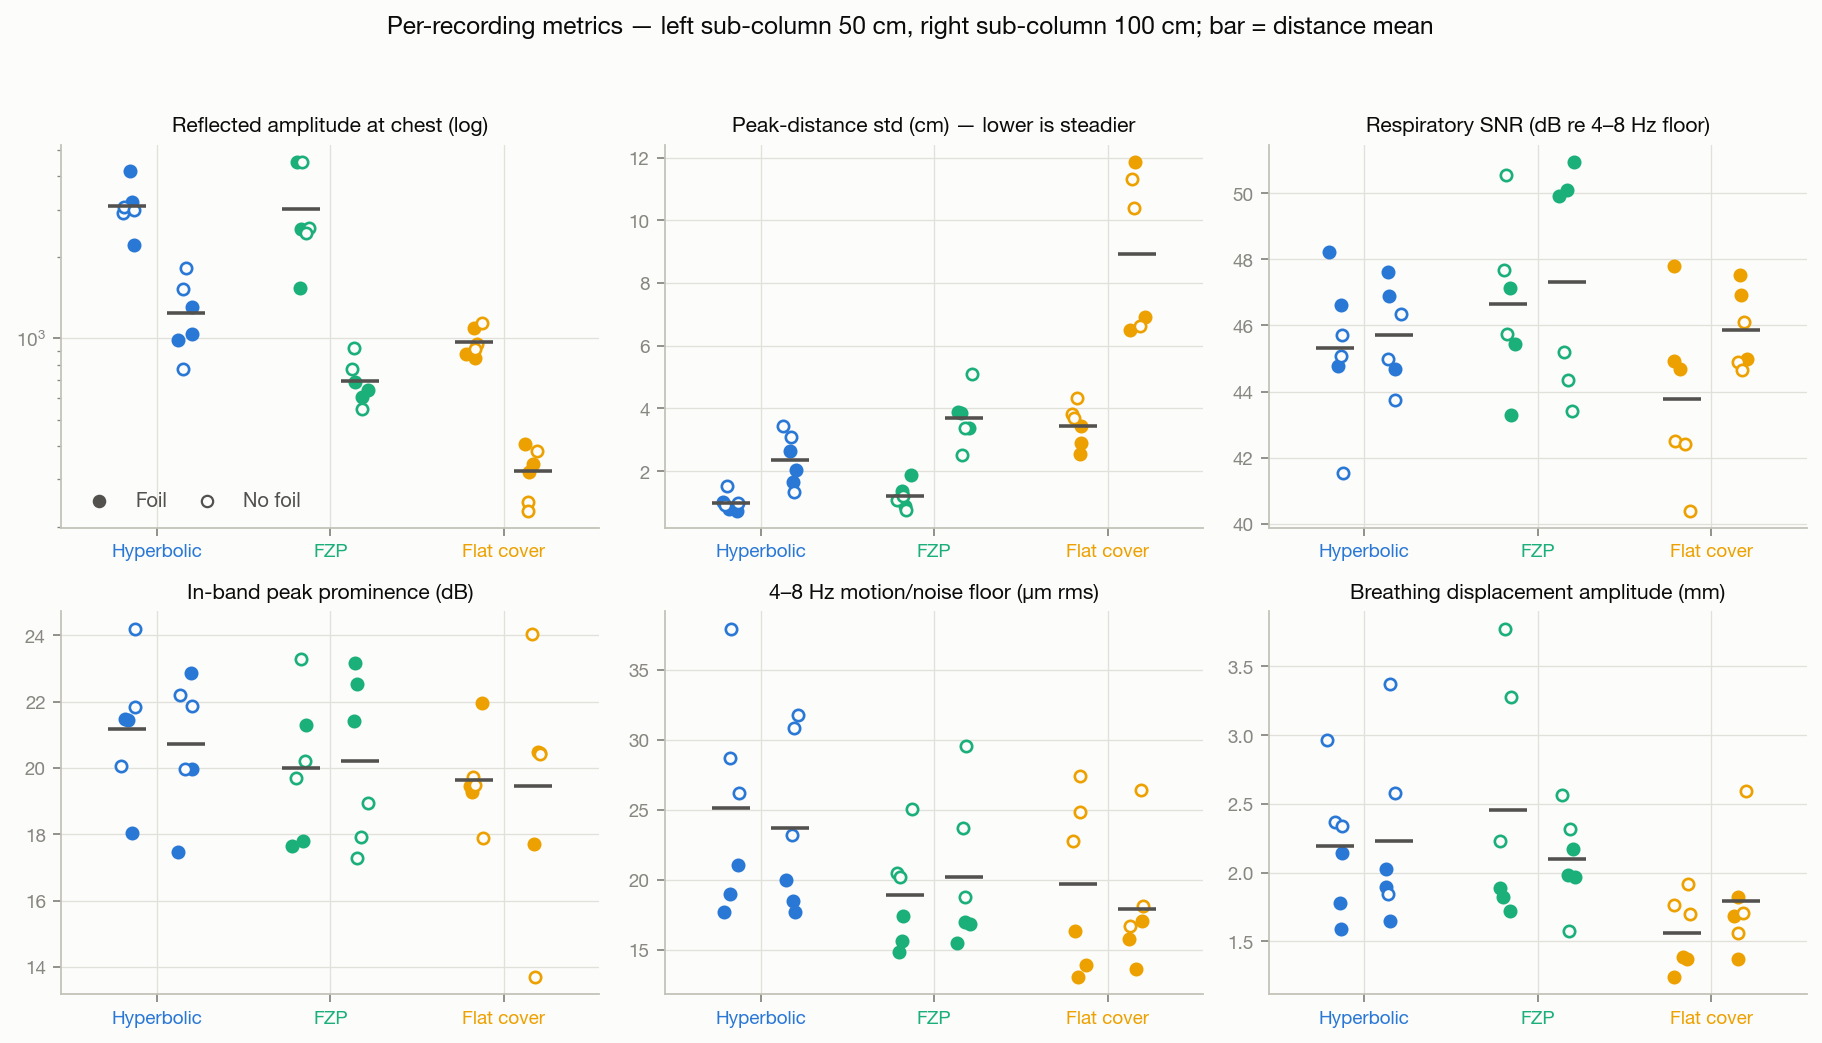
\includegraphics[width=\textwidth]{foil_metryki.png}
    \caption[Zestawienie metryk dla wszystkich nagrań]{Wszystkie metryki dla
    36~nagrań. Każdy punkt oznacza jedną próbę; punkty wypełnione --- folię,
    puste --- brak folii, a~lewa/prawa podkolumna w~obrębie soczewki ---
    odpowiednio \SI{50}{cm}/\SI{100}{cm}. Pozioma kreska jest średnią dla
    danego dystansu z~obu stanów folii i~trzech powtórzeń. W~panelach amplitudy,
    SNR, wyrazistości piku i~przemieszczenia większa wartość oznacza silniejszą
    składową; dla odchylenia odległości i~szumu \SIrange{4}{8}{Hz} korzystna
    jest wartość mniejsza. Amplituda i~stabilność śledzenia wyraźnie różnicują
    soczewki, natomiast SNR i~wyrazistość piku --- nie.}
    \label{fig:metryki}
\end{figure}

Dodatkowo zaobserwowano, że płaska pokrywa \emph{zaniża} amplitudę
przemieszczenia oddechowego (1,6--1,8~mm wobec 2,1--2,5~mm dla soczewek
skupiających, $p \leq 0{,}009$) --- szeroka wiązka uśrednia fazę po dużym,
niejednorodnie poruszającym się obszarze tułowia.

\section{Wyniki: wpływ folii aluminiowej}

\begin{table}[H]
\centering
\caption{Parowane różnice (folia $-$ brak folii) dopasowane po soczewce,
odległości i~numerze powtórzenia (18~par, test Wilcoxona).}
\label{tab:folia}
\small
\begin{tabular}{@{}lrrr@{}}
\toprule
Metryka & Mediana różnicy & Folia lepsza & $p$ \\
\midrule
Amplituda odbicia & $-0{,}5$~dB & 8/18 & 0,64 \\
SNR oddechowy & $+2{,}5$~dB & 13/18 & \textbf{0,012} \\
Szum ruchowy \SIrange{4}{8}{Hz} & $-9{,}1$~\si{\micro\metre} & 1/18 & $<0{,}0001$ \\
Amplituda przemieszczenia & $-0{,}46$~mm & 4/18 & 0,001 \\
Stabilność odległości & $-0{,}18$~cm & 6/18 & 0,18 \\
Wyrazistość piku & $\approx 0$ & 10/18 & 0,87 \\
\bottomrule
\end{tabular}
\end{table}

\begin{figure}[H]
    \centering
    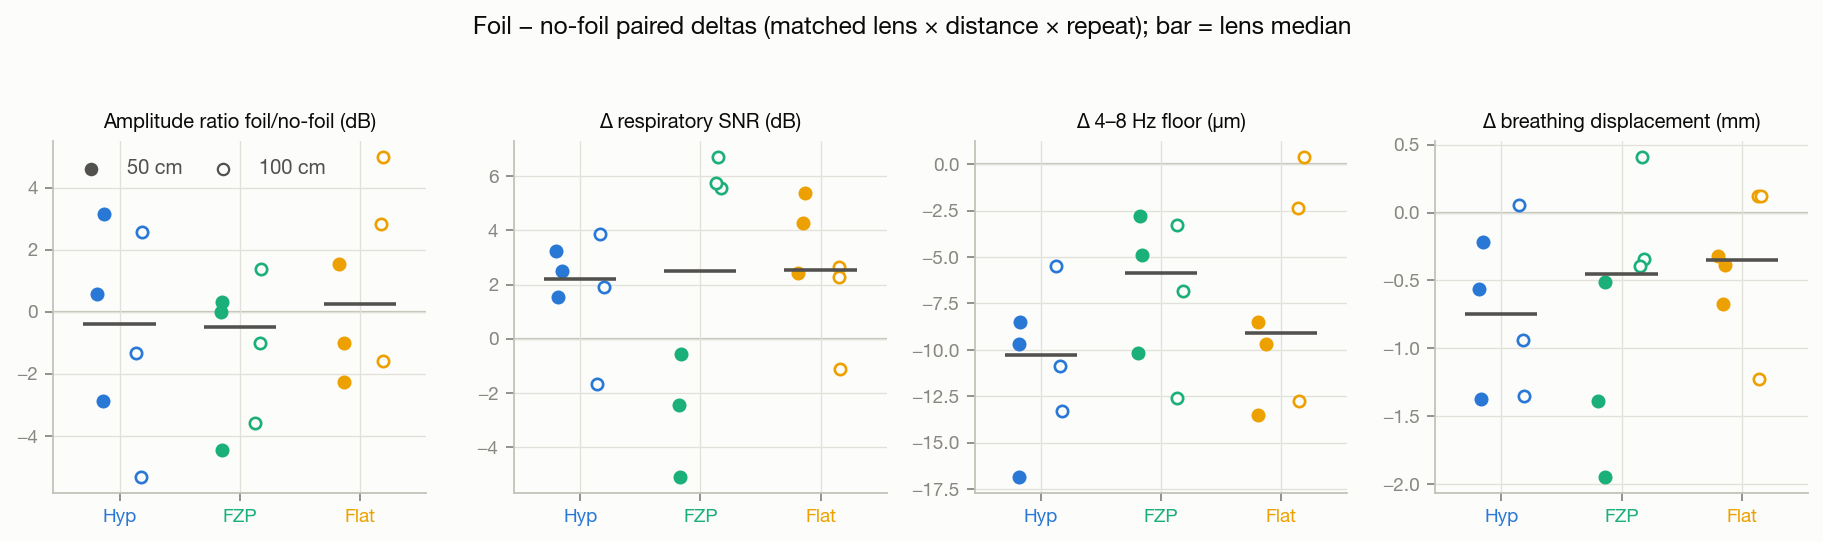
\includegraphics[width=\textwidth]{foil_delty_parowane.png}
    \caption[Parowane różnice dla folii aluminiowej]{Parowane różnice
    folia~$-$~brak folii po dopasowaniu soczewki, dystansu i~numeru
    powtórzenia. Każdy punkt jest jedną parą; punkty wypełnione oznaczają
    \SI{50}{cm}, puste \SI{100}{cm}, pozioma kreska --- medianę dla soczewki,
    a~linia zera --- brak zmiany. Dodatnia wartość oznacza wzrost danej
    metryki z~folią; w~panelu szumu wartość ujemna jest więc korzystna.
    Amplituda oscyluje wokół zera, natomiast podobny dla wszystkich soczewek
    spadek szumu jest sygnaturą różnicy sesji, a~nie selektywnego działania
    reflektora.}
    \label{fig:delty}
\end{figure}

\paragraph{Nie zaobserwowano oczekiwanego wzrostu amplitudy.} Łata z~folii
miała działać przez zwiększenie odbicia, lecz różnica amplitudy oscyluje wokół
zera (mediana $-0{,}5$~dB, 8/18~par na korzyść folii, $p = 0{,}64$) dla każdej
soczewki i~obu odległości. Dane wskazują więc, że na dystansie
\SIrange{50}{100}{cm} wkład łaty o~boku \SI{5}{cm} nie dał mierzalnego wzrostu
na tle odbicia od całego tułowia. Ze względu na rozdzielenie sesji nie można
jednak z~tych danych wyznaczyć czystego efektu folii na SNR.

\paragraph{Znaczenie kąta padania.} Geometria stanowiska mogła dodatkowo
osłabić oczekiwany efekt metalowej łaty. Przy kącie około
\SI{30}{\degree} względem normalnej silna składowa zwierciadlana odbicia od
przewodzącej powierzchni może zostać skierowana poza antenę odbiorczą zamiast
wrócić do radaru. Folia przylegała do niepłaskiej, poruszającej się powierzchni
ciała, dlatego nie można traktować jej jak idealnego lustra, ale wynik dotyczy
właśnie tej realistycznej geometrii siedzącej. Stały sposób ustawienia we
wszystkich warunkach nie zaburza porównania soczewek, ogranicza natomiast
uogólnienie wniosku o~folii na padanie prostopadłe.

\paragraph{Pozorna poprawa SNR to prawdopodobnie efekt sesji.} Wzrost SNR
o~2,5~dB jest istotny statystycznie, ale wynika wyłącznie z~\emph{mianownika}:
poziom szumu ruchowego w~paśmie \SIrange{4}{8}{Hz} był niższy w~17~z~18~par,
i~to w~podobnym stopniu dla wszystkich trzech soczewek --- także dla płaskiej
pokrywy, gdzie fizyka wiązki czyniłaby ewentualny wkład folii najsłabszym.
Jednocześnie amplituda przemieszczenia oddechowego również była niższa w~sesji
z~folią. Najprostsze wyjaśnienie: badany siedział spokojniej i~oddychał
płycej podczas pierwszej sesji z~folią niż podczas drugiej sesji bez folii. Prawdziwego
mechanizmu (folia tłumiąca mikroruchy skóry) nie da się całkowicie wykluczyć,
ale przewidywałby on wzrost amplitudy i~zależność od soczewki --- żadne z~tych
zjawisk nie występuje.

\begin{figure}[H]
    \centering
    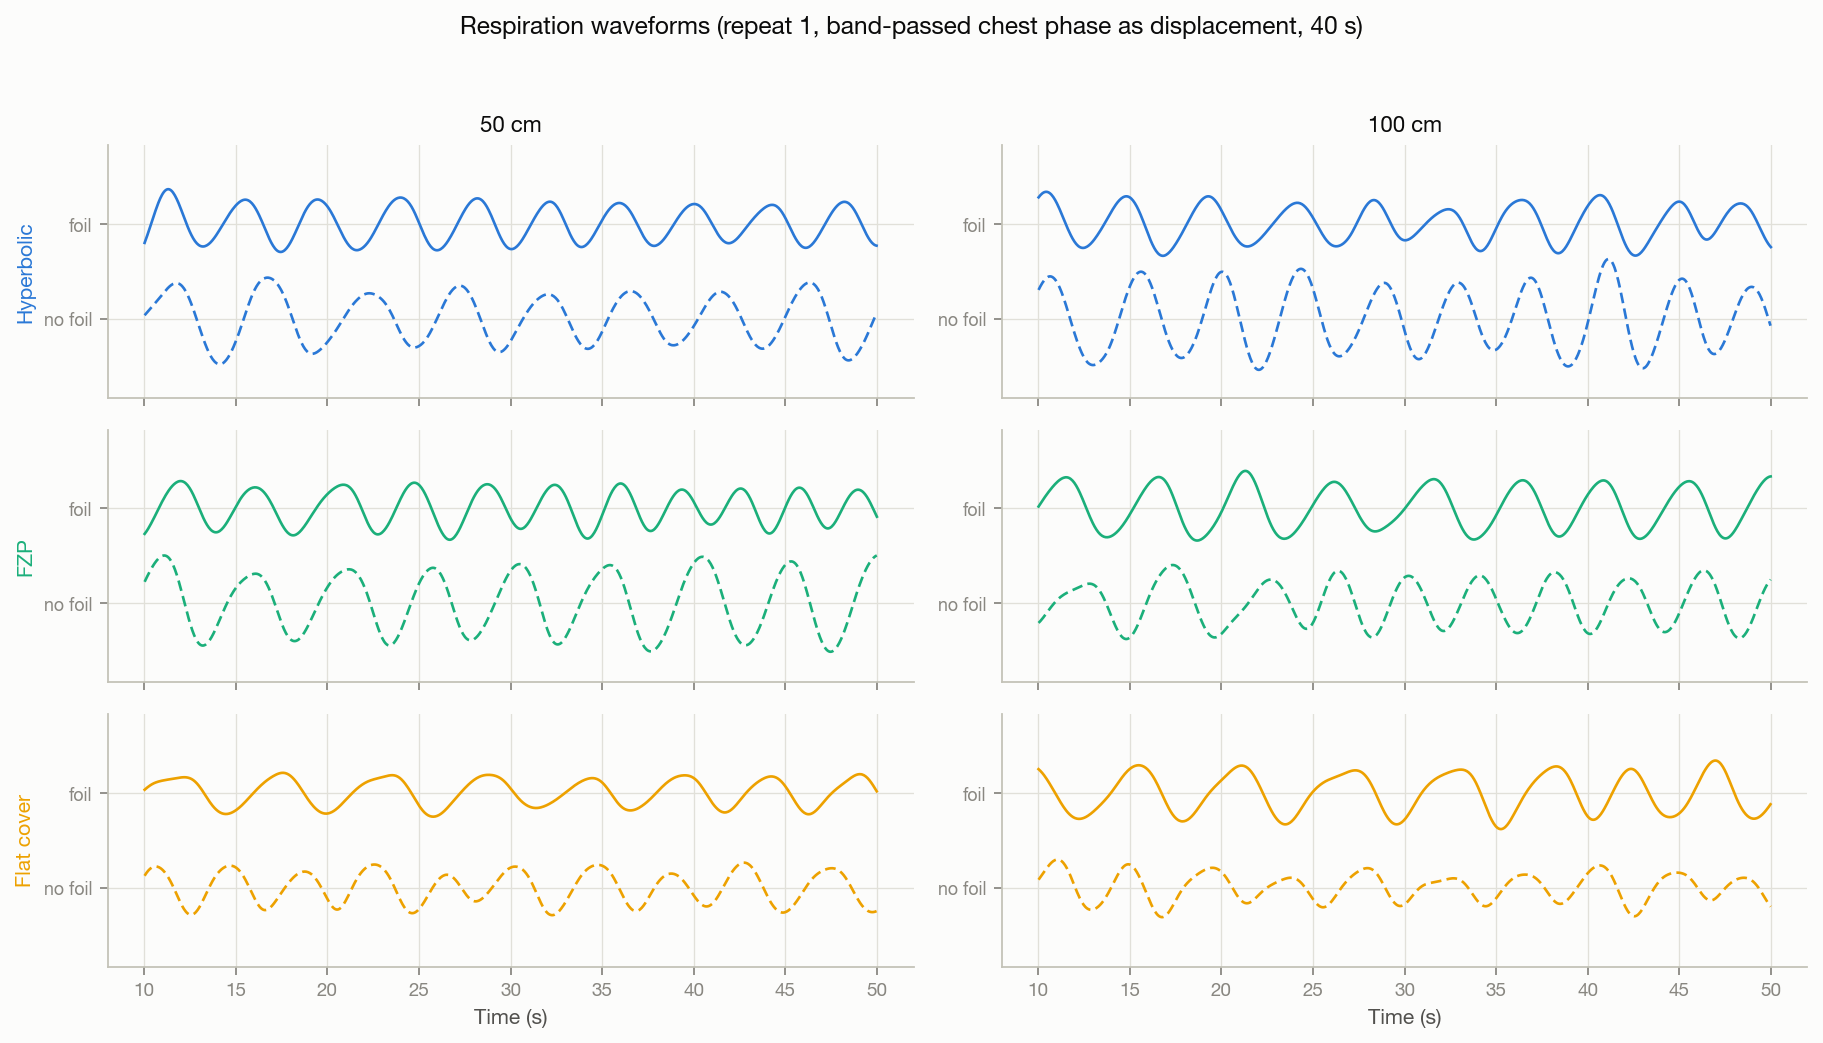
\includegraphics[width=\textwidth]{foil_przebiegi_oddechu.png}
    \caption[Przebiegi oddechowe]{40~sekund przefiltrowanego sygnału
    przemieszczenia klatki piersiowej (fragment \SIrange{10}{50}{s}) z~pierwszego
    powtórzenia każdego z~12~warunków. Wiersze odpowiadają soczewkom, kolumny
    dystansom, linia ciągła oznacza folię, a~przerywana jej brak. Przebiegi
    przesunięto pionowo, aby się nie nakładały, dlatego ich poziom zerowy nie
    ma znaczenia; porównywać należy amplitudę i~regularność. Wszystkie są
    czytelne, lecz płaska pokrywa daje wyraźnie mniejszą amplitudę ruchu.}
    \label{fig:przebiegi}
\end{figure}

\section{Wnioski z eksperymentu}
\begin{enumerate}
  \item Na dystansie \SIrange{0.5}{1.0}{m} system \emph{nie jest ograniczony
  amplitudą} --- SNR oddechowy wynosi 44--47~dB niezależnie od konfiguracji.
  Dodatkowa moc odbita przekłada się na \emph{stabilność śledzenia celu},
  a~nie na wykrywalność oddechu.
  \item Soczewka hiperboliczna jest najlepszym wyborem domyślnym: najlepiej
  utrzymuje amplitudę na większym dystansie i~najstabilniej śledzi cel.
  \item Na dystansie \SIrange{0.5}{1.0}{m} nie wykazano wzrostu amplitudy
  dzięki folii. Rozdzielenie warunków na dwie sesje uniemożliwia natomiast
  przypisanie folii zaobserwowanej różnicy SNR. Praktyczna korzyść przy małym
  zapasie sygnału pozostaje nierozstrzygnięta.
  \item Wskaźniki pewności wbudowane w~pipeline (\emph{resp\_confidence},
  \emph{signal\_quality}) osiągają wartości maksymalne we wszystkich 36
  nagraniach, przez co nie różnicują warunków --- do oceny jakości sygnału
  konieczne są miary widmowe.
\end{enumerate}

\section{Retest folii i kąta padania na dystansie 2 m}
\label{sec:folia-2m}

\subsection{Plan pomiaru}

Retest wykonano wyłącznie z~soczewką hiperboliczną, ponieważ
poprzedni eksperyment wskazał ją jako najpewniejszy wariant na większy
dystans. Zastosowano układ $2\times2$: naturalna pozycja siedząca z~osią
radaru poziomą (około \SI{30}{\degree} od normalnej do klatki) oraz ustawienie
prawie prostopadłe, każde bez folii i~z~folią. Warunki oznaczono odpowiednio
\texttt{N0}, \texttt{NF}, \texttt{P0} i~\texttt{PF}. Każdy z~nich powtórzono
trzykrotnie, uzyskując 12~zaakceptowanych nagrań po \SI{90}{s}
(1801--1802~ramek, około \SI{20}{Hz}). Radar obejmował zakres
\SIrange{1.5}{2.5}{m}, używał profilu~3, HWAAS~32 i~ośmiu przemiatań na
ramkę.

Odległość nominalną \SI{2}{m} ustawiono dalmierzem MILESEEY~D2. W~pozycji
naturalnej poziome ustawienie osi kontrolowano poziomnicą pęcherzykową.
W~pozycji prawie prostopadłej kąt weryfikowano zwrotem plamki lasera na
kartkę odniesienia przy dalmierzu: powrót w~pobliże punktu emisji oznaczał,
że normalna do lokalnego fragmentu powierzchni była zbliżona do osi radaru.
Nie jest to laboratoryjny pomiar kąta płaskiej próbki --- klatka i~przylegająca
folia są zakrzywione --- lecz kontrola usuwa główny błąd polegający na
skierowaniu odbicia zwierciadlanego poza odbiornik. Łata miała ponownie
wymiary $\SI{5}{cm}\times\SI{5}{cm}$, a~jej górna krawędź znajdowała się
\SI{5}{cm} poniżej linii łączącej brodawki sutkowe.

Najpierw wykonano wszystkie próby z~folią, a~następnie wszystkie bez folii,
aby przykleić i~zdjąć łatę tylko raz. Dokładna kolejność wynosiła
\texttt{NF, PF, PF, NF, NF, PF, P0, N0, N0, P0, P0, N0}; geometrie były więc
przeplatane wewnątrz każdego bloku, ale stan folii pozostaje całkowicie
splątany z~czasem sesji. Wyniki folii są z~tego powodu opisowe, natomiast
porównanie kąta jest znacznie lepiej zabezpieczone przed monotonicznym dryfem.

Sekwencję generował programowy przewodnik oddechu z~sekcji
\ref{sec:programowy-przewodnik-oddechu}. Każde nagranie zawierało ten sam protokół:
\SI{10}{s} oddechu swobodnego,
7~cykli sterowanych (wdech \SI{2}{s}, wydech \SI{3}{s}), \SI{15}{s}
wstrzymania oddechu po wydechu i~6~kolejnych cykli sterowanych. Zadana
częstość wynosiła więc dokładnie \SI{0.20}{Hz}, czyli
12~oddechów/min.

\subsection{Rekonstrukcja sygnału i synchronizacja komend}

Dla każdego nagrania wyznaczono medianowy profil amplitudy IQ i~bramkę celu.
W~otoczeniu $\pm\SI{20}{cm}$ od celu zachowano bramki o~medianowej amplitudzie
co najmniej 25\% lokalnego maksimum, rozpleciono ich fazę, usunięto trend
liniowy i~obliczono średnią ważoną amplitudą. Fazę przeliczono na ruch
radialny zależnością $x=\lambda\varphi/(4\pi)$ dla częstotliwości
\SI{60.5}{GHz}, po czym zastosowano zerofazowy filtr Butterwortha drugiego
rzędu \SIrange{0.10}{0.50}{Hz}.

Znaczników z~aplikacji nie nałożono bezpośrednio na czas ramek. Dla odcinków
sterowanych utworzono trójkątny wzorzec zgodny z~konwencją znaku ustaloną
w~sekcji~\ref{sec:model-sygnalu}: faza maleje podczas wdechu i~rośnie
podczas wydechu. Wzorca tego nie dopasowywano co do znaku --- korelacja
wyszła dodatnia we~wszystkich 12~nagraniach, co potwierdza, że konwencja jest
stałą właściwością toru. Następnie dla każdej próby szukano przesunięcia w~kroku
\SI{25}{ms}, które maksymalizowało korelację Pearsona między wzorcem
i~sygnałem. Oszacowane łączne opóźnienie komenda--zarejestrowany ruch mieściło
się w~zakresie \SIrange{0.275}{0.625}{s}, z~medianą \SI{0.375}{s}. Maksima
rozpoczynające wdech występowały medianowo \SI{0.273}{s} po komendzie, a~minima
kończące wdech --- \SI{0.499}{s} po komendzie. Różnica wskazuje, że oddech nie
jest jedynie idealnym wzorcem przesuniętym w~czasie: badany reaguje szybko,
ale domyka ruch wdechowy nieco później.

Oszacowanie obejmuje łącznie reakcję człowieka, opóźnienie akwizycji
i~przetwarzanie A121. Pliki nie zawierają wspólnego sprzętowego znacznika
komendy i~emisji ramki, dlatego tych składowych nie można rozdzielić.
Zerofazowy filtr użyty offline nie wnosi natomiast dodatkowego przesunięcia
fazowego. Na rys.~\ref{fig:foil2m-przebiegi} granice faz przesunięto osobno
dla każdego nagrania o~jego oszacowane $\delta$.

\begin{figure}[p]
    \centering
    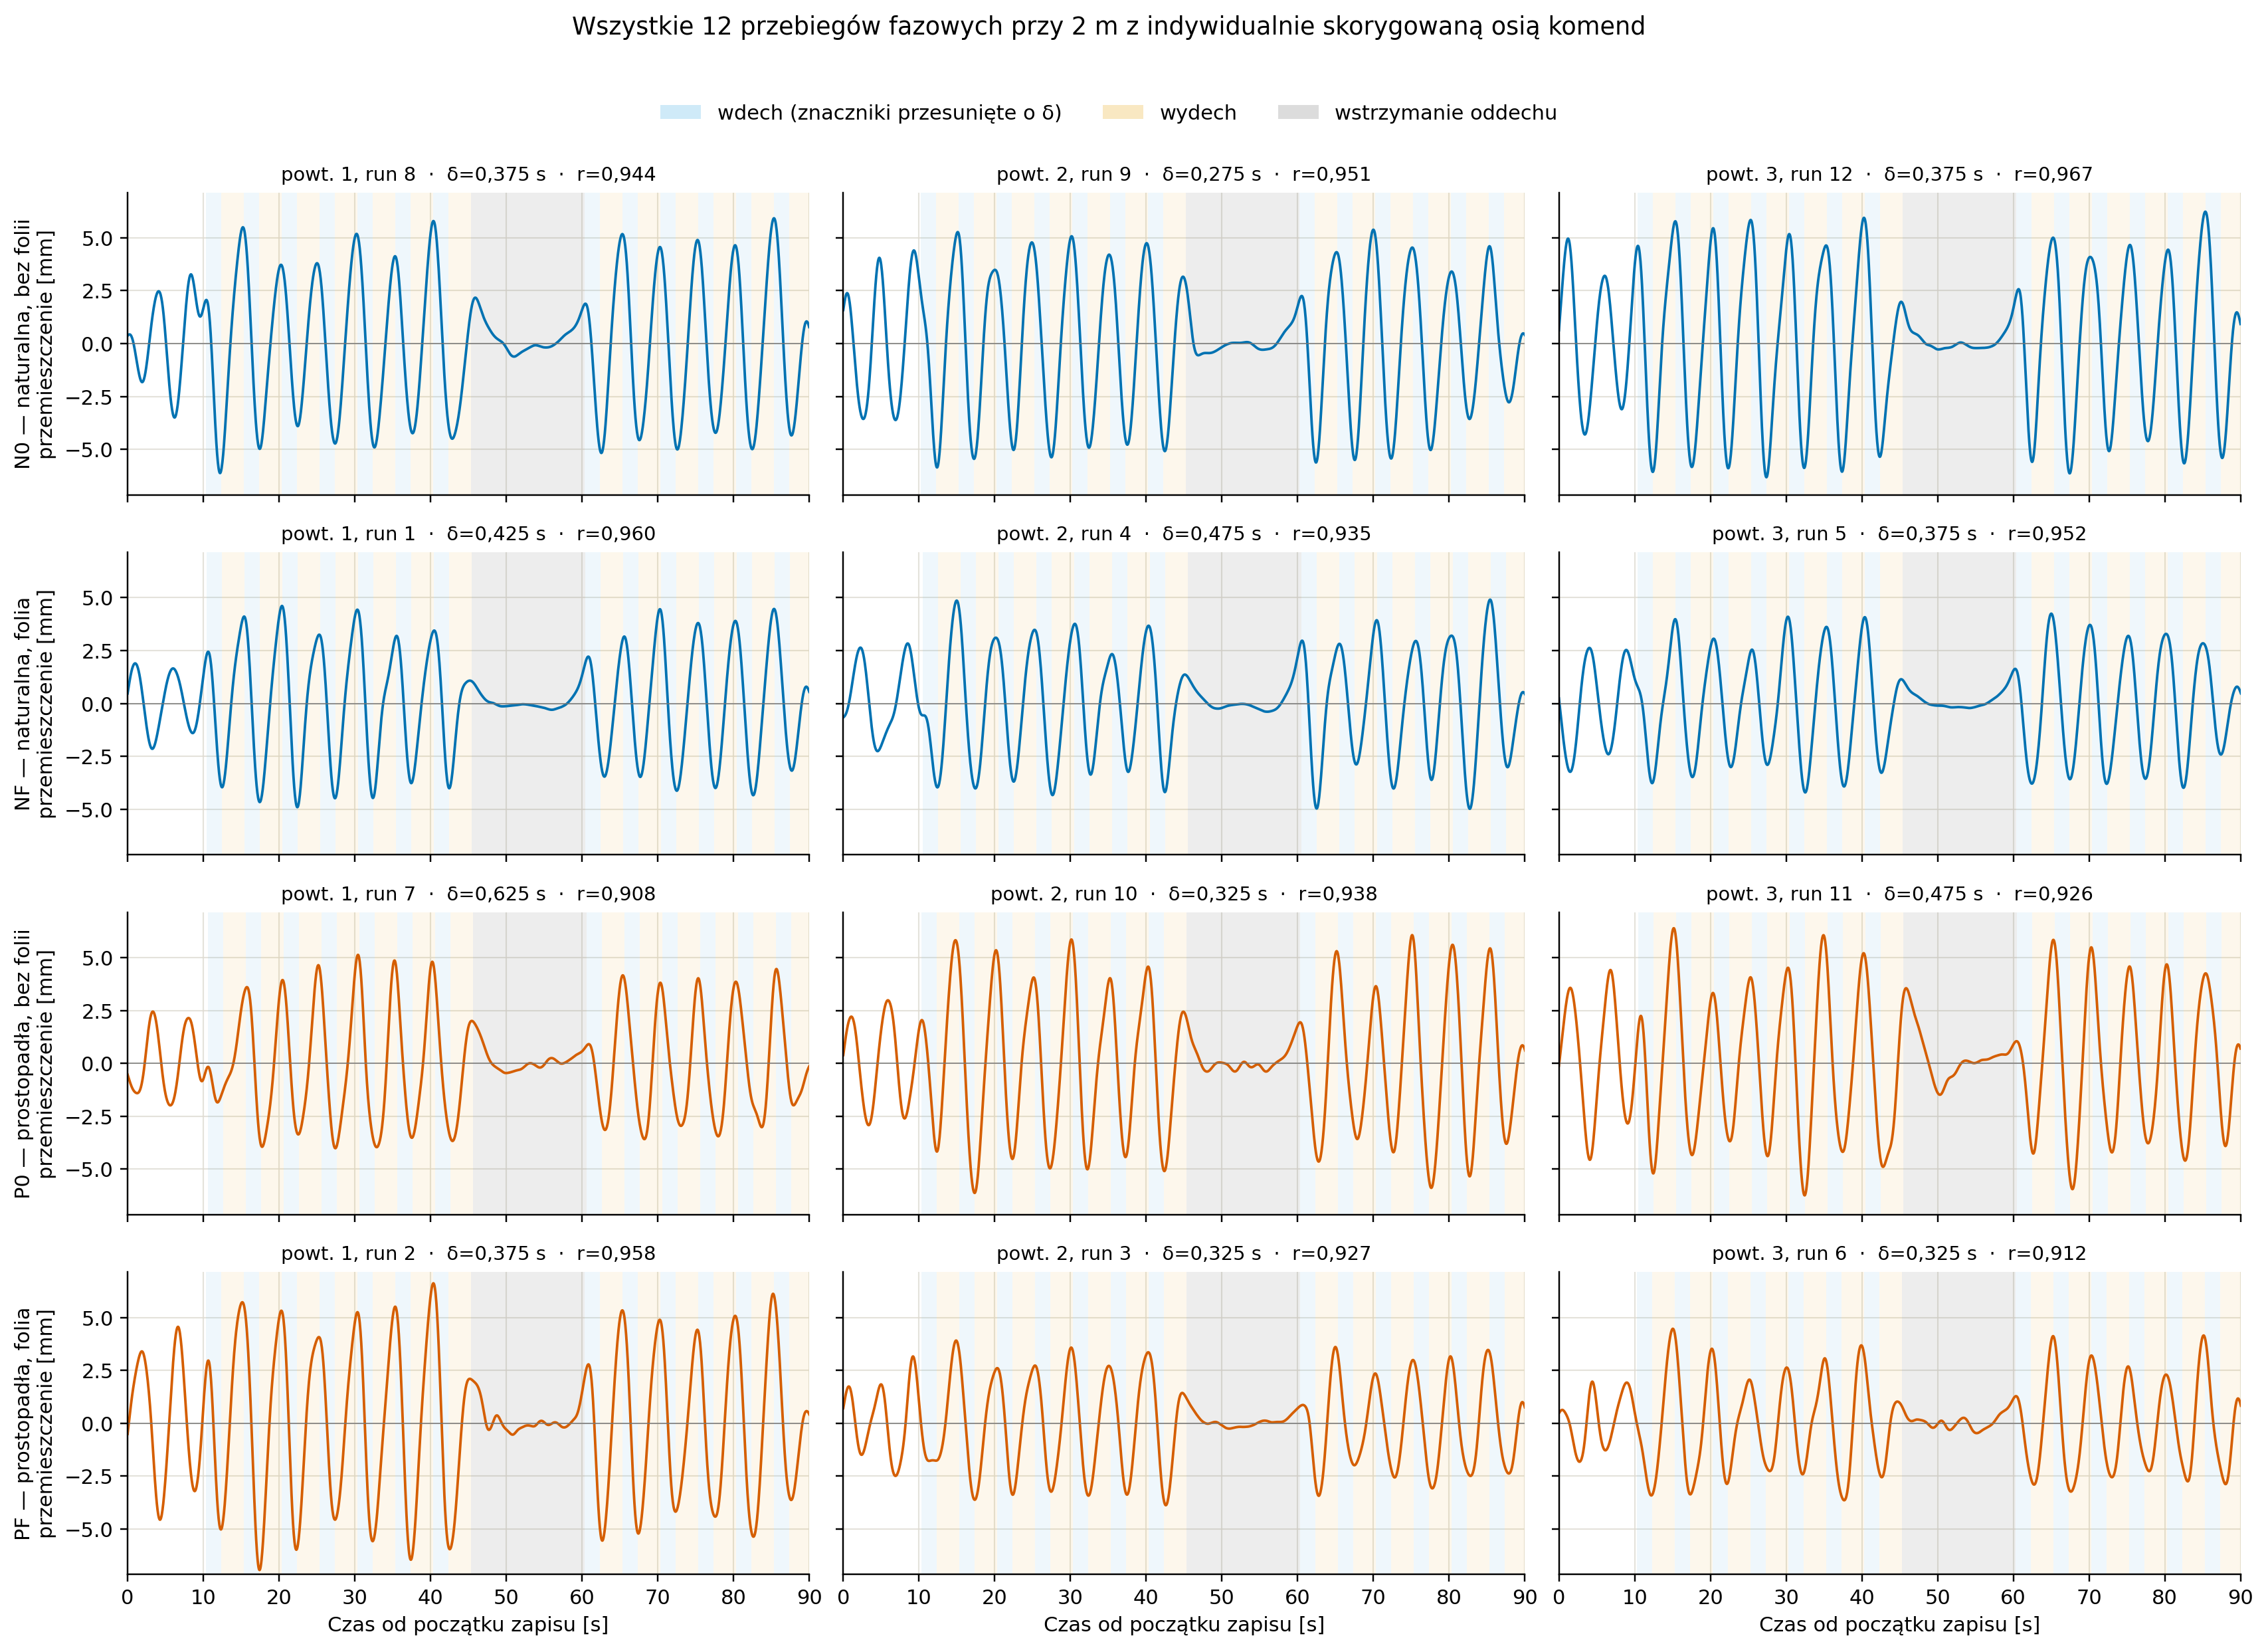
\includegraphics[width=\textwidth]{foil2m_przebiegi_fazy.png}
    \caption[Przebiegi A121 przy 2 m z fazami komend]{Wszystkie 12~przebiegów
    przemieszczenia oddechowego przy \SI{2}{m}. Wiersze odpowiadają warunkom,
    a~kolumny numerom powtórzeń; nad panelem podano numer w~kolejności sesji,
    indywidualne przesunięcie $\delta$ i~korelację $r$. Tło niebieskie oznacza
    wdech, pomarańczowe wydech, a~szare wstrzymanie. Wspólna skala pionowa
    ujawnia zarówno różnice głębokości oddechu, jak i~silny zanik ruchu
    w~środkowej części wstrzymania.}
    \label{fig:foil2m-przebiegi}
\end{figure}

\subsection{Wyniki retestu}

\begin{table}[H]
\centering
\caption{Mediany z~trzech powtórzeń każdego warunku przy \SI{2}{m}.
$\sigma_d$ jest odchyleniem standardowym położenia dominującego piku,
$A_{\mathrm{od}}$ --- połową zakresu między 5. i~95. percentylem ruchu
w~odcinkach sterowanych, a~\emph{hold} --- $20\log_{10}$ ilorazu RMS fazy
oddechowej w~środkowych \SI{9}{s} wstrzymania i~RMS podczas oddychania.}
\label{tab:folia-2m}
\small
\begin{tabular}{@{}lrrrrrrr@{}}
\toprule
Warunek & Echo & Bramka & $\sigma_d$ & $r$ & $\delta$ & $A_{\mathrm{od}}$ & Hold \\
 & [j.u.] & [m] & [cm] & [--] & [s] & [mm] & [dB] \\
\midrule
\texttt{N0} &  501 & 2,002 & 5,31 & 0,951 & 0,375 & 4,78 & $-23{,}7$ \\
\texttt{NF} &  543 & 2,012 & 5,37 & 0,952 & 0,425 & 3,76 & $-24{,}3$ \\
\texttt{P0} & 2247 & 1,872 & 1,06 & 0,926 & 0,475 & 4,83 & $-20{,}0$ \\
\texttt{PF} & 2068 & 1,842 & 1,25 & 0,927 & 0,325 & 3,18 & $-23{,}6$ \\
\bottomrule
\end{tabular}
\end{table}

\begin{figure}[H]
    \centering
    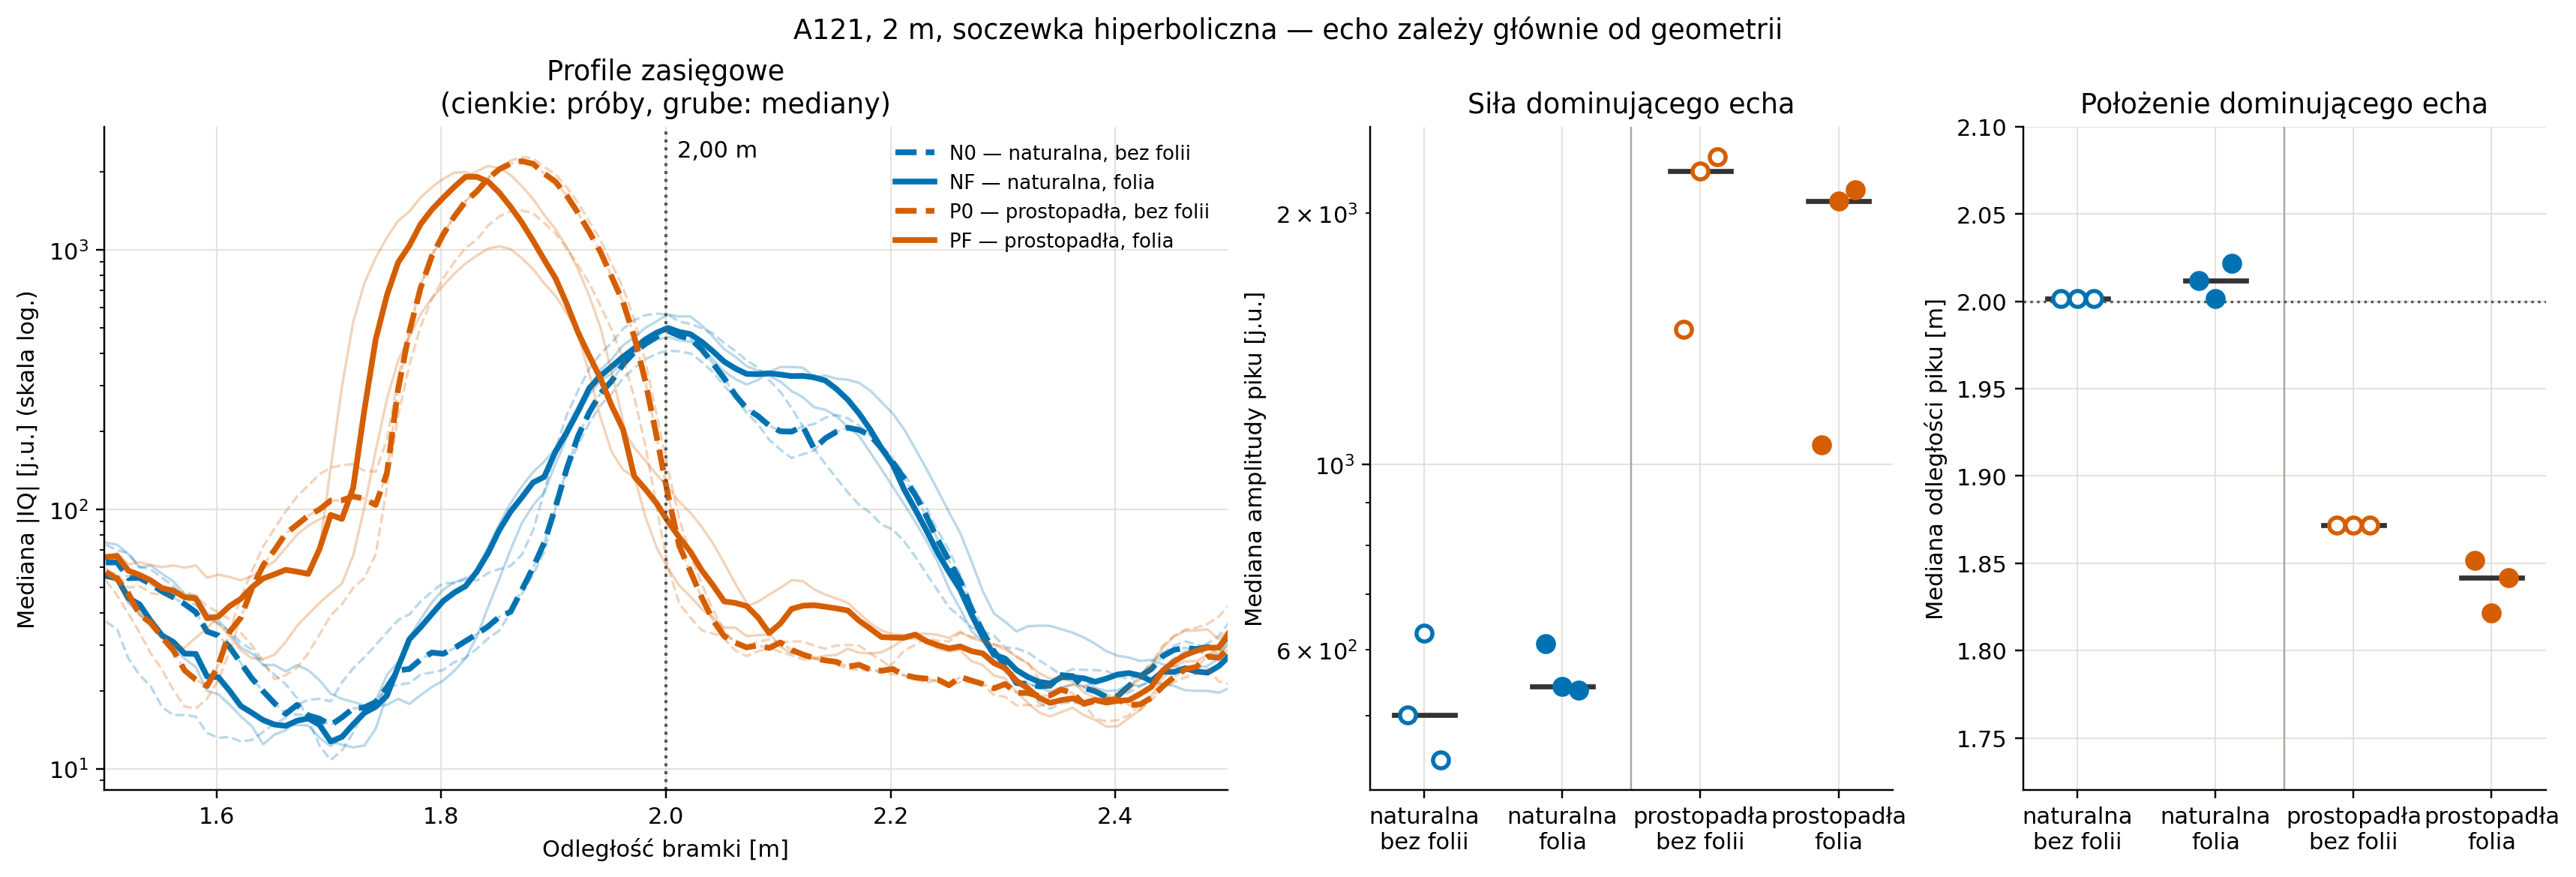
\includegraphics[width=\textwidth]{foil2m_profile_i_echo.png}
    \caption[Profile i amplituda echa przy 2 m]{Profile zasięgowe i~echo przy
    \SI{2}{m}. W~lewym panelu cienka krzywa jest medianą po czasie z~jednej
    próby, a~gruba medianą trzech prób; linie niebieskie oznaczają pozycję
    naturalną, pomarańczowe prawie prostopadłą, ciągłe folię, a~przerywane jej
    brak. Linia pionowa wskazuje dystans nominalny ustawiony dalmierzem.
    Środkowy panel pokazuje medianową amplitudę dominującego piku, prawy jego
    położenie; punkty to próby, a~czarne kreski mediany warunków.}
    \label{fig:foil2m-profile}
\end{figure}

\paragraph{Kąt padania zdominował amplitudę echa.} Po sparowaniu po numerze
powtórzenia przejście z~ustawienia naturalnego do prawie prostopadłego
zwiększało amplitudę o~medianę \SI{11.06}{dB} bez folii i~\SI{11.62}{dB}
z~folią, czyli odpowiednio około 3,6 i~3,8~raza w~skali amplitudowej IQ.
Wynik nie ogranicza się do wysokości piku: mediana $\sigma_d$ zmalała
z~około \SI{5.3}{cm} w~pozycji naturalnej do \SIrange{1.1}{1.3}{cm}
w~pozycji prostopadłej. Właściwe skierowanie wąskiej wiązki dawało zatem
silniejsze i~stabilniej zlokalizowane echo.

Dominująca bramka przesunęła się jednocześnie z~około \SI{2.01}{m} do
\SIrange{1.84}{1.87}{m}. Dystans z~A121 nie jest tym samym pomiarem co odczyt
dalekomierza do zaznaczonego punktu: po zmianie osi radaru maksimum może
pochodzić z~innego fragmentu zakrzywionego tułowia, a~bezwzględne położenie
bramki zależy też od profilu czujnika. Z~tego powodu wzrostu o~\SI{11}{dB}
nie należy przypisywać wyłącznie idealnemu prawu odbicia od tej samej płaskiej
powierzchni. Jest to łączny, lecz praktycznie istotny efekt poprawnego
wycelowania stanowiska.

\begin{figure}[H]
    \centering
    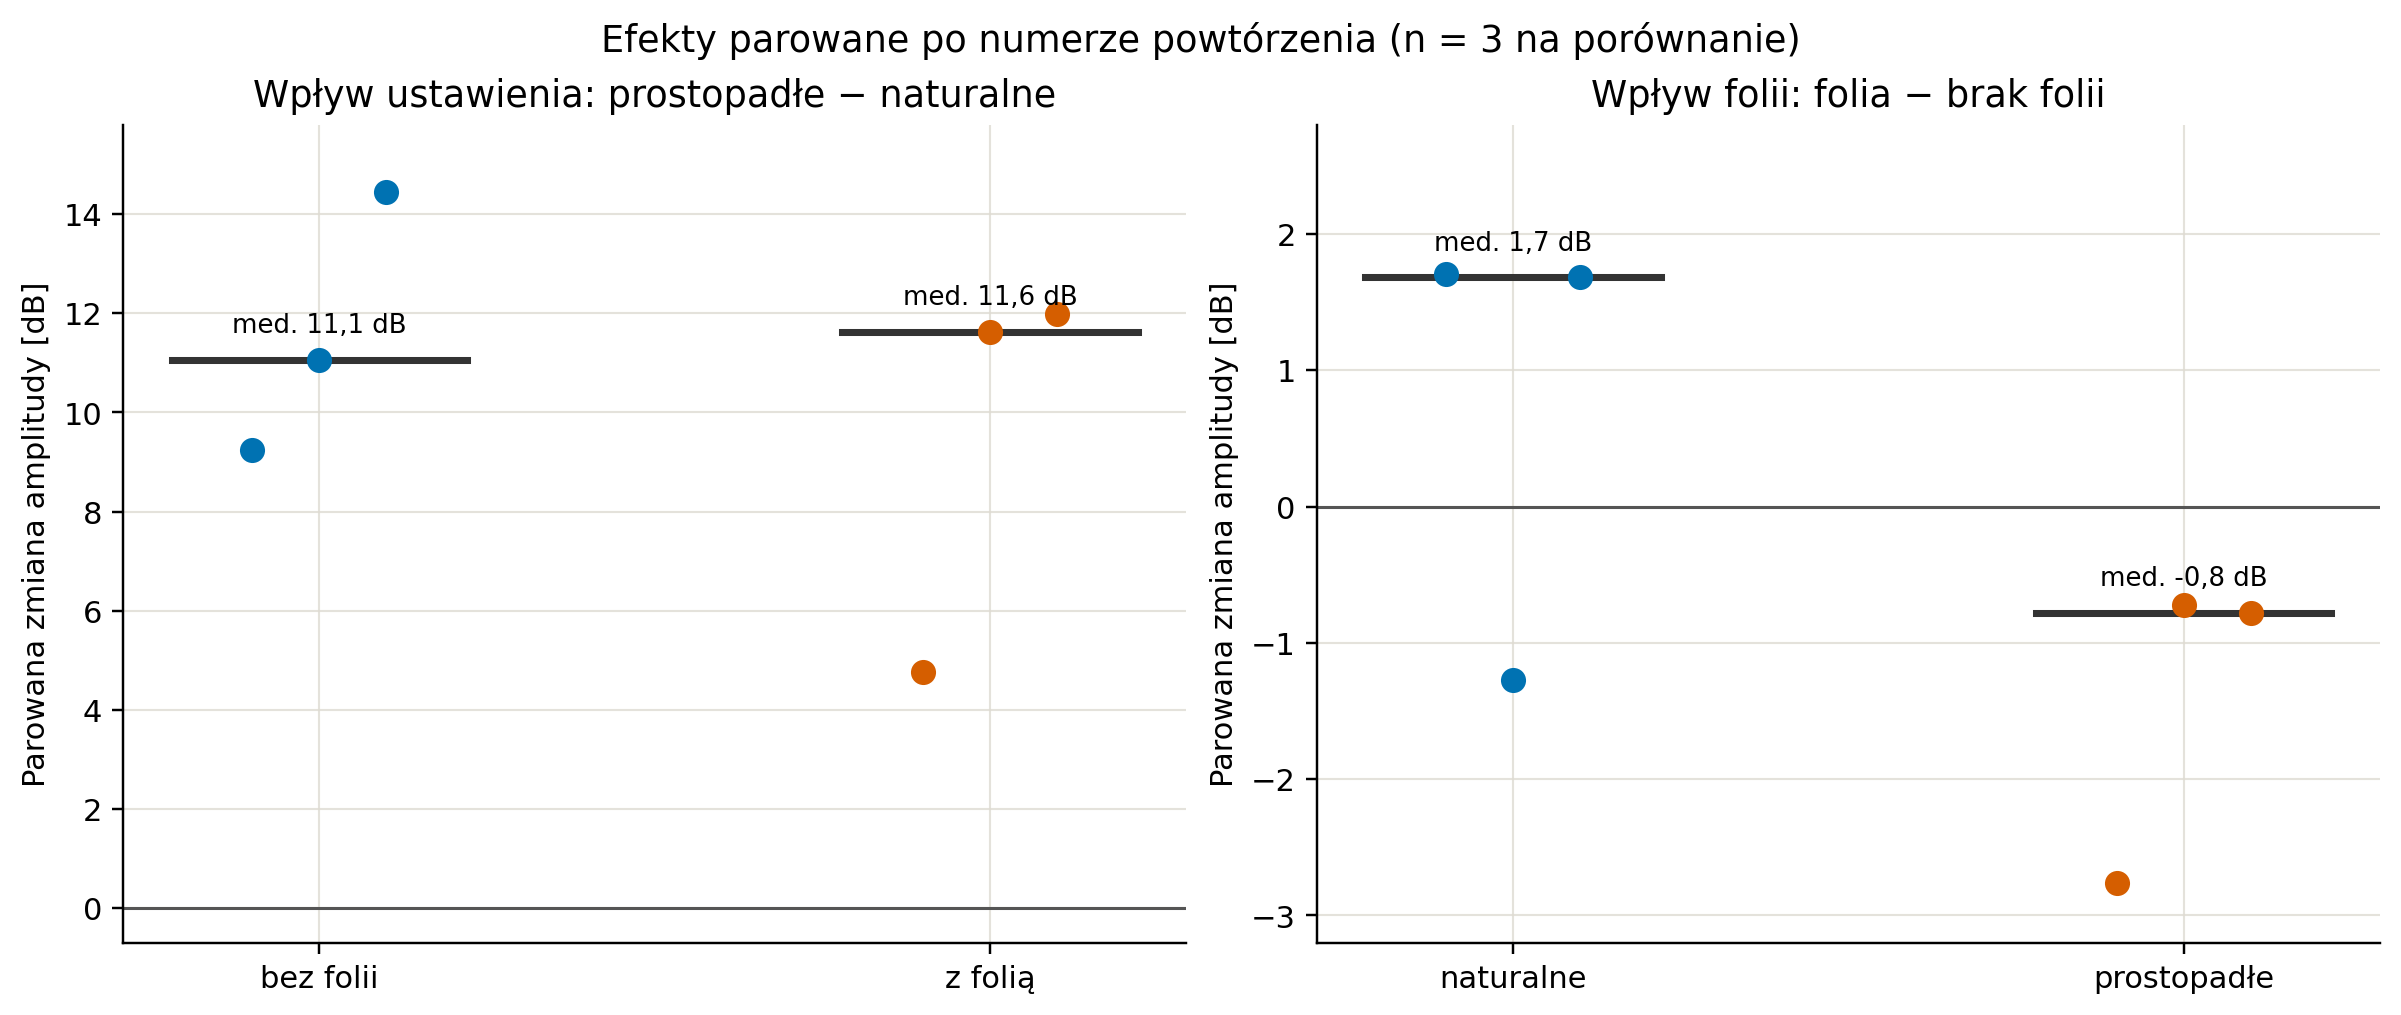
\includegraphics[width=0.92\textwidth]{foil2m_efekty_parowane.png}
    \caption[Parowane efekty kąta i folii przy 2 m]{Zmiana medianowej amplitudy
    echa po sparowaniu warunków po numerze powtórzenia. Lewy panel pokazuje
    efekt ustawienia prostopadłego względem naturalnego, prawy --- efekt folii
    względem braku folii. Każdy punkt jest jednym powtórzeniem, kreska jego
    medianą dla danej geometrii lub stanu folii. Kąt daje duży efekt o~zgodnym
    znaku; niewielki efekt folii zmienia znak między geometriami.}
    \label{fig:foil2m-efekty}
\end{figure}

\paragraph{Folia nie dała powtarzalnego wzmocnienia.} W~pozycji naturalnej
parowane zmiany amplitudy wyniosły $+1{,}71$, $-1{,}28$ i~$+1{,}68$~dB
(mediana $+1{,}68$~dB). W~ustawieniu prawie prostopadłym, w~którym powrót
zwierciadlany powinien najbardziej sprzyjać metalowej łacie, wszystkie trzy
zmiany były ujemne: $-2{,}77$, $-0{,}72$ i~$-0{,}78$~dB (mediana
$-0{,}78$~dB). Nie ma więc zgodnego efektu folii między dwiema geometriami.
Ponieważ cały blok z~folią poprzedzał blok bez folii, nie można utożsamiać
małych różnic z~czystym skutkiem materiału; można natomiast odrzucić
praktycznie duże, jednoznaczne wzmocnienie oczekiwane od reflektora.

\begin{figure}[H]
    \centering
    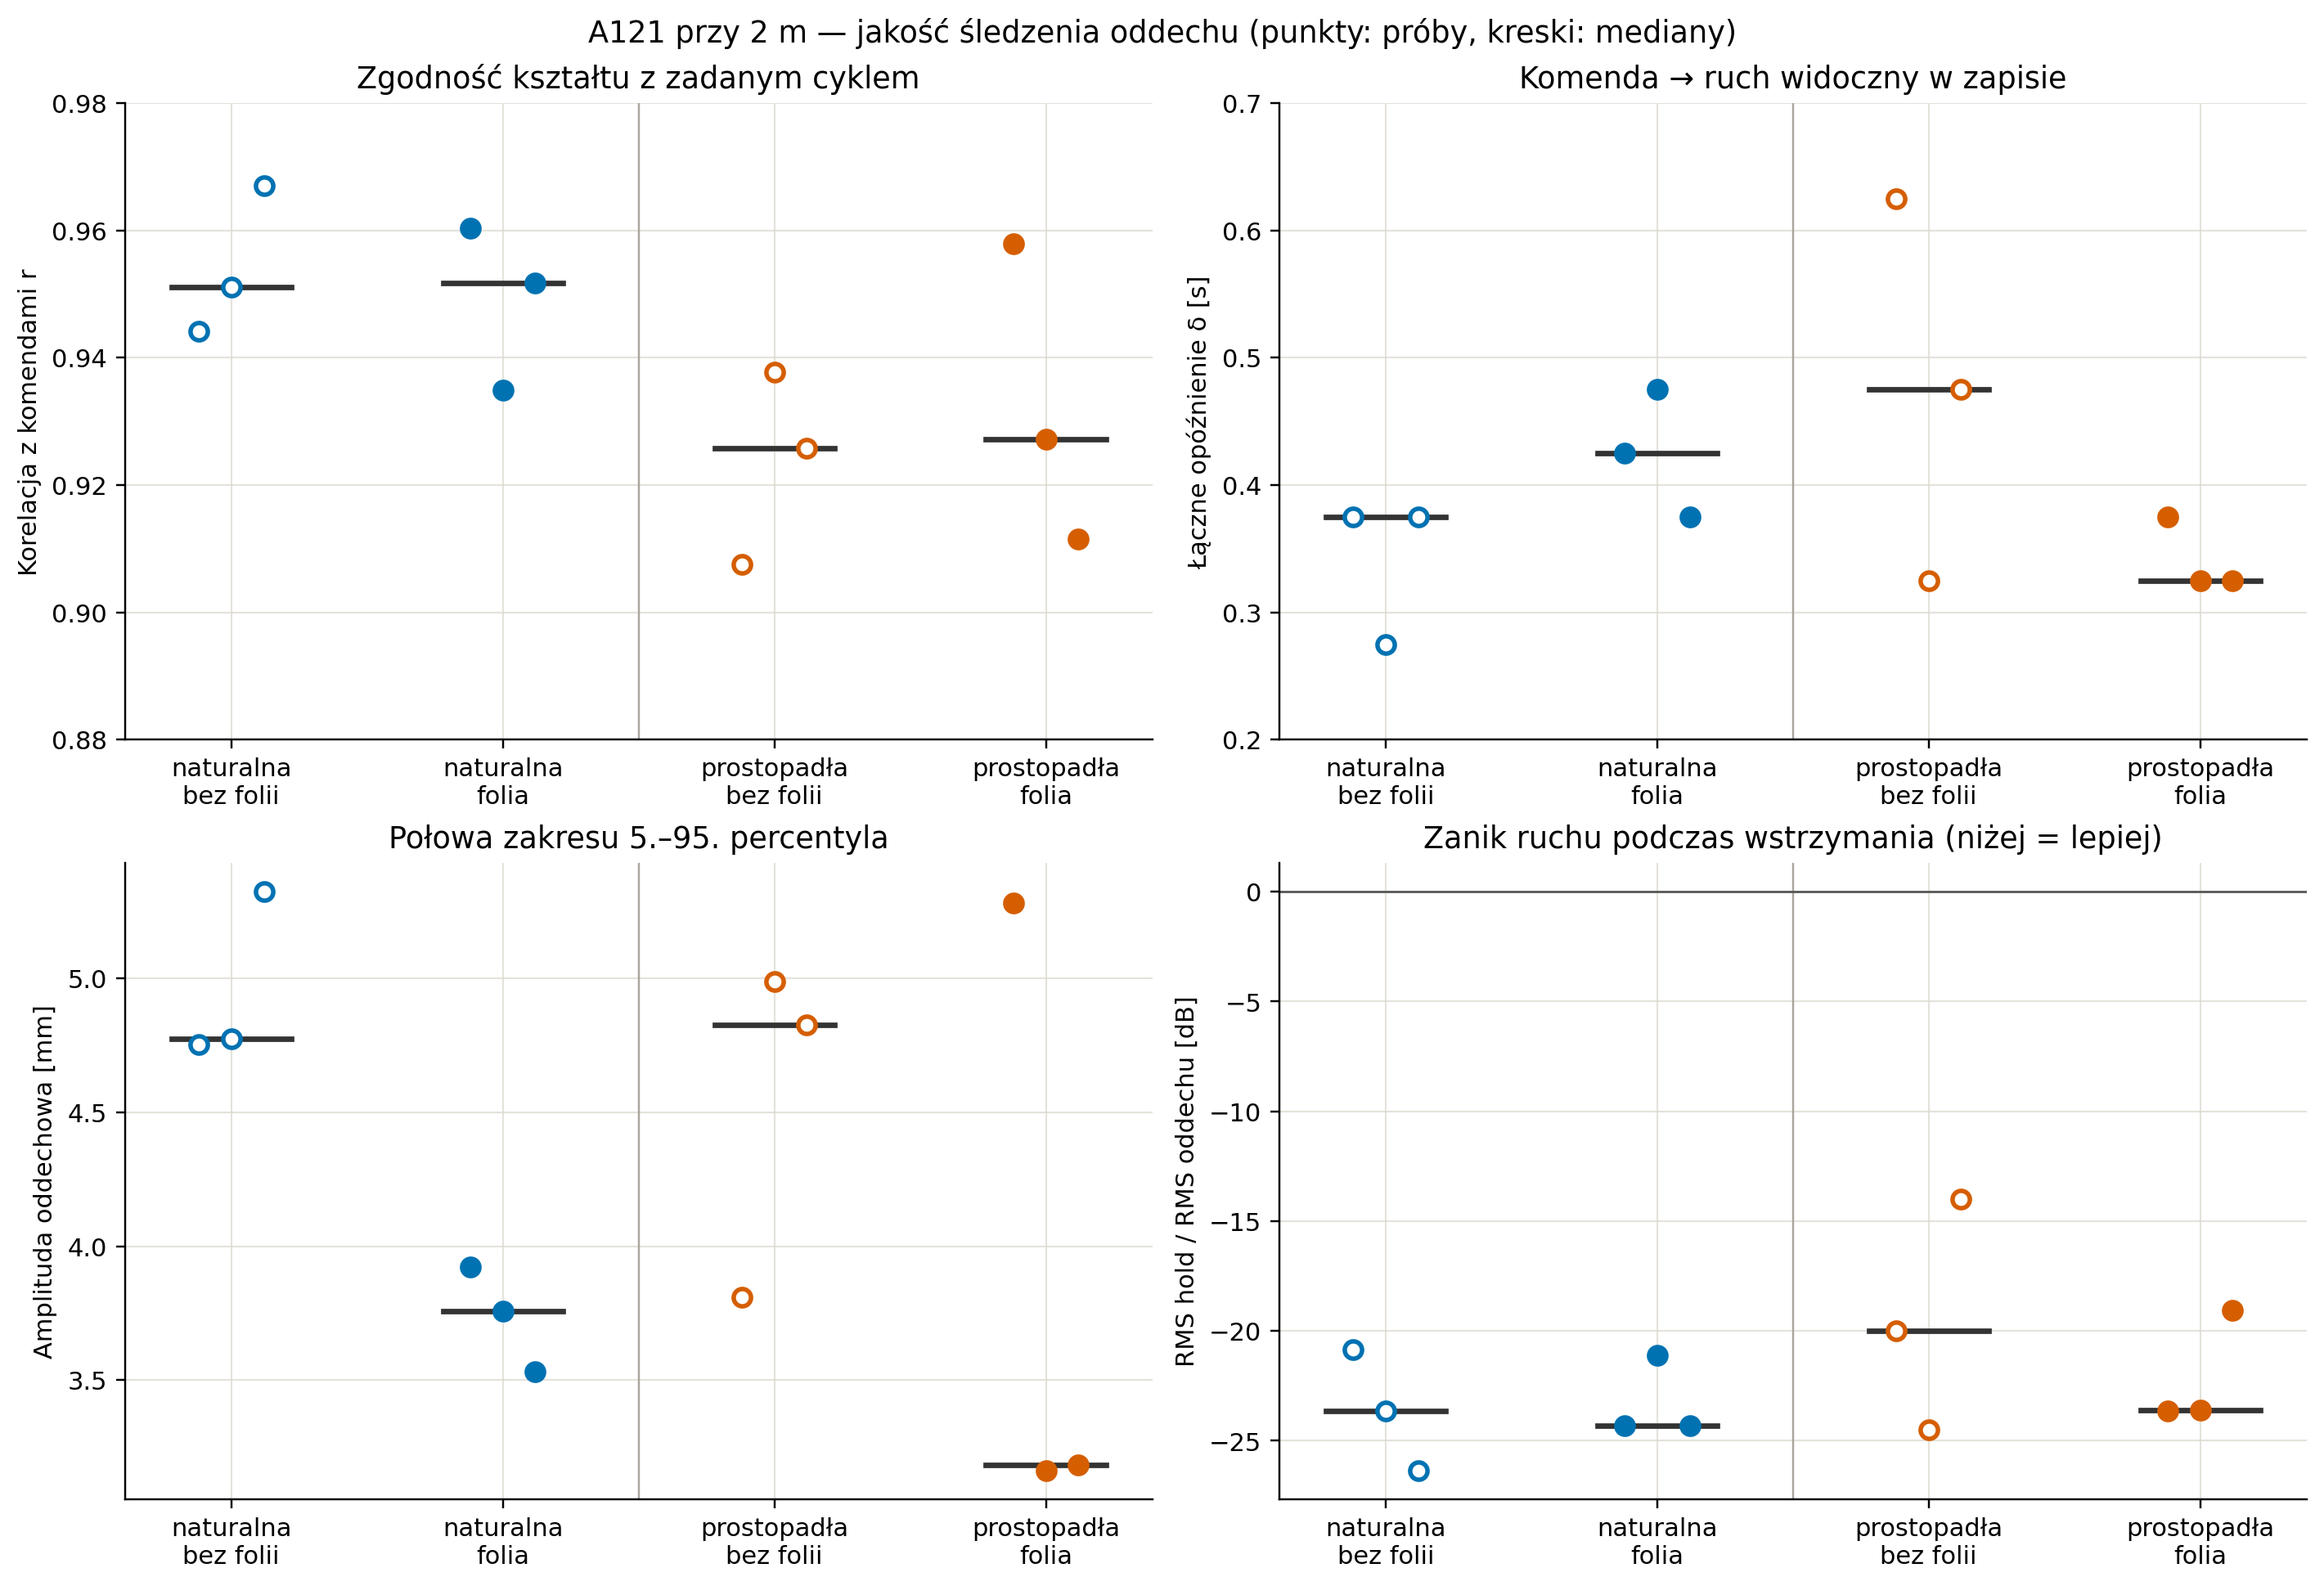
\includegraphics[width=\textwidth]{foil2m_metryki_sygnalu.png}
    \caption[Metryki sygnału oddechowego A121 przy 2 m]{Metryki sygnału
    oddechowego przy \SI{2}{m}; punkty oznaczają próby, kreski mediany,
    wypełnienie punktu folię, a~pusty punkt jej brak. Korelacja dotyczy
    trójkątnego wzorca po korekcie $\delta$. Amplituda jest miarą głębokości
    zarejestrowanego oddechu, nie siły echa. W~prawym dolnym panelu bardziej
    ujemna wartość oznacza silniejszy zanik ruchu podczas wstrzymania.}
    \label{fig:foil2m-metryki}
\end{figure}

\paragraph{Oddech był użyteczny we wszystkich 12 próbach.} Korelacja ze
wzorcem po korekcie opóźnienia wynosiła od $0{,}908$ do $0{,}967$. Częstość
wyznaczona z~odstępów między maksimami mieściła się w~zakresie
11,86--12,10~oddechów/min, bardzo blisko zadanych 12~oddechów/min. Amplituda
radialnego ruchu oddechowego wynosiła
\SIrange{3.16}{5.32}{mm}. W~środkowych \SI{9}{s} wstrzymania RMS w~paśmie
oddechowym malał o~\SIrange{14.0}{26.3}{dB}, czyli od około 5 do 21~razy
w~skali amplitudy. Zanik jest widoczny w~każdej próbie, a~trzysekundowe
marginesy od granic wstrzymania ograniczają wpływ reakcji badanego i~dzwonienia
filtru wokół gwałtownej zmiany ruchu.

Większe echo nie przełożyło się wprost na większą zgodność faz oddechu.
Mediany $r$ wynosiły $0{,}951$--$0{,}952$ w~pozycji naturalnej i~
$0{,}926$--$0{,}927$ w~prostopadłej, mimo około czterokrotnie większej
amplitudy IQ w~drugiej geometrii. Przy zaledwie trzech powtórzeniach nie jest
to dowód przewagi pozycji naturalnej, lecz potwierdzenie wcześniejszej
obserwacji: po przekroczeniu progu użyteczności siła echa i~wierność przebiegu
są różnymi cechami.

W~zapisanym strumieniu aplikacja referencyjna A121 podawała mediany
11,41--12,12~oddechów/min; niezerowy wynik był dostępny
w~54,8--83,2\% ramek, co obejmuje czas początkowego ustalania celu i~celowe
wstrzymanie. Dla próby \texttt{P0}, powtórzenie~2, podsumowanie wykonane po
zakończeniu zapisało 0~BPM, ponieważ ostatnie ramki przeszły do stanu
\texttt{DETERMINE\_DISTANCE\_ESTIMATE}. Nie oznaczało to utraty oddechu:
mediana wartości zapisanych wcześniej wynosiła 11,82~oddechów/min,
korelacja offline $0{,}938$, a~częstość z~ekstremów 11,98~oddechów/min.
Przypadek pokazuje, że pojedynczy stan
końcowy aplikacji nie powinien zastępować analizy całego przebiegu.

\subsection{Wnioski z retestu}

\begin{enumerate}
  \item A121 z~soczewką hiperboliczną rejestrował sterowany oddech i~jego
  zatrzymanie z~dystansu \SI{2}{m} we wszystkich czterech warunkach.
  \item Prawie prostopadłe ustawienie zwiększało echo o~około \SI{11}{dB}
  i~stabilizowało położenie piku. Dokładne wycelowanie radaru jest zatem
  ważniejsze niż dodanie niewielkiej metalowej łaty.
  \item Nie wykazano użytecznego wzmocnienia przez folię ani przy naturalnym,
  ani przy prawie prostopadłym padaniu. Wniosek o~małym efekcie jest zgodny
  z~testem \SIrange{0.5}{1.0}{m}.
\end{enumerate}

% ---------------------------------------------------------------------
\chapter{Sieci neuronowe do analizy faz oddechu}
\label{chap:sieci}

\todo{Rozdział jeszcze nie zrealizowany --- kluczowa część pracy,
do wykonania. Poniżej planowana struktura; zarezerwowano dużo miejsca.}

\section{Sformułowanie zadania}
\miejsce{Klasyfikacja faz cyklu oddechowego (wdech / wydech / pauza) z~sygnału
fazowego radaru A121. Alternatywnie: regresja fazy cyklu lub detekcja zdarzeń
oddechowych.}

\section{Zbiór danych i anotacja}
\miejsce{Wykorzystanie zgromadzonej bazy nagrań (nagrania sterowane
i~całonocne). Istniejący moduł \texttt{a121\_breaths} realizuje automatyczną
wstępną anotację oddechów --- opisać jej zasadę i~sposób weryfikacji ręcznej.
Podział na zbiór uczący / walidacyjny / testowy (rozłączny względem nagrań).}

\section{Architektura modelu}
\miejsce{Proponowane architektury: 1D-CNN na oknach sygnału, sieć
rekurencyjna (LSTM/GRU), ewentualnie model hybrydowy. Wejście: przefiltrowany
sygnał fazowy i/lub spektrogram. Uzasadnienie wyboru.}

\section{Uczenie i metryki}
\miejsce{Funkcja straty, augmentacja danych, walidacja krzyżowa po nagraniach.
Metryki: dokładność klasyfikacji faz, F1, błąd wyznaczenia momentów przejścia.}

\section{Wyniki}
\miejsce{Tabele i~wykresy wyników; porównanie z~metodą klasyczną
(baseline oparty na detekcji pików z~rozdziału~\ref{chap:algorytmy}).}

\section{Dyskusja}
\miejsce{Ograniczenia (jeden badany, ograniczona liczba nagrań), możliwości
uogólnienia, potencjał zastosowania w~czasie rzeczywistym.}

% =====================================================================
% =====================================================================
\part{Zastosowanie systemu}
\label{part:eksperymenty}
% =====================================================================
% =====================================================================

\chapter{Całonocny monitoring snu}
\label{chap:sen}

\section{Cel badania}
Docelowym zastosowaniem zbudowanego systemu jest bezkontaktowy monitoring snu.
W~tej części radar A121 wykorzystano do rejestracji pełnych nocy, a~uzyskane
przebiegi tętna, oddechu oraz oszacowane fazy snu porównano z~danymi
z~zegarka Garmin~Fenix~7, który służył jako konsumencki punkt odniesienia,
a~nie jako wzorzec kliniczny.

\section{Metodyka pomiarów}
Zarejestrowano serię nagrań całonocnych w~dwóch ustawieniach stanowiska.
Równolegle badany nosił zegarek Garmin~Fenix~7. W~lokalnym archiwum
zweryfikowano zestawy FIT dla trzech nocy głównego porównania, niepełnego
zapisu pilotażowego i~negatywnego przypadku geometrii; każdy zestaw
zawiera pliki \texttt{WELLNESS}, \texttt{SLEEP\_DATA} oraz pozostałe metryki
snu. Do głównego porównania wybrano trzy \emph{pełne} nagrania, dla których
dostępne są jednocześnie dane A121 i~Garmina:
\begin{itemize}
  \item noc~1 --- soczewka plano-convex, radar przy krawędzi łóżka,
  \item noc~2 --- soczewka FZP, radar przy krawędzi łóżka,
  \item noc~3 --- płaska pokrywa (efektywnie brak soczewki), radar na
  wysięgniku nad łóżkiem.
\end{itemize}

Niepełnego zapisu pilotażowego nie użyto w~wynikach, ponieważ tę samą
konfigurację płaskiej pokrywy reprezentuje pełna i~lepiej udokumentowana
noc~3. Dla dodatkowych pełnych nocy~4 i~5 zachowały się
dane radarowe, lecz w~archiwum nie ma odpowiadających im eksportów FIT;
wykorzystano je wyłącznie do oceny powtarzalności stanowiska.

W~nocach~1 i~2 radar znajdował się przy bocznej krawędzi łóżka, około
\SI{10}{cm} nad górną powierzchnią materaca, a~jego oś była równoległa do
podłoża. Takie ustawienie jest zbliżone do prostopadłego względem klatki tylko
wtedy, gdy badany leży na boku i~pozostaje na wysokości czujnika. Po obrocie na
plecy, przesunięciu w~głąb łóżka albo zmianie ułożenia tułowia oś przestaje
trafiać w~ten sam fragment klatki. Jest to szczególnie niekorzystne dla
węższych wiązek soczewek skupiających i~wyjaśnia, dlaczego początkowo poprawne
wycelowanie nie gwarantowało dobrej jakości przez całą noc.

W~trzech pełnych nagraniach oznaczonych jako noce~3--5 zastosowano
płaską pokrywę oraz ustawienie nad łóżkiem pokazane na
rys.~\ref{fig:stanowisko-sen}. Statyw Manfrotto stał obok łóżka, a~poziomy
wysięgnik wprowadzał czujnik nad tułów. Głowicę skierowano w~dół, w~przybliżeniu
pod kątem \SI{45}{\degree} względem powierzchni materaca, na środkową część
klatki piersiowej. Mediany odległości celu śledzonego przez A121 wynosiły
odpowiednio \SI{0.30}{m}, \SI{0.37}{m} i~\SI{0.39}{m}. Stanowisko opisano więc
jako dystans około \SI{0.4}{m}, zmienny wraz z~pozycją ciała i~ułożeniem
pościeli, a~nie jako odległość wyznaczoną z~dokładnością dalmierza. Szerokie
pole widzenia płaskiej pokrywy obejmowało większą część tułowia i~lepiej
tolerowało nocne przesunięcia niż ustawienie przy krawędzi łóżka.

\begin{figure}[H]
    \centering
    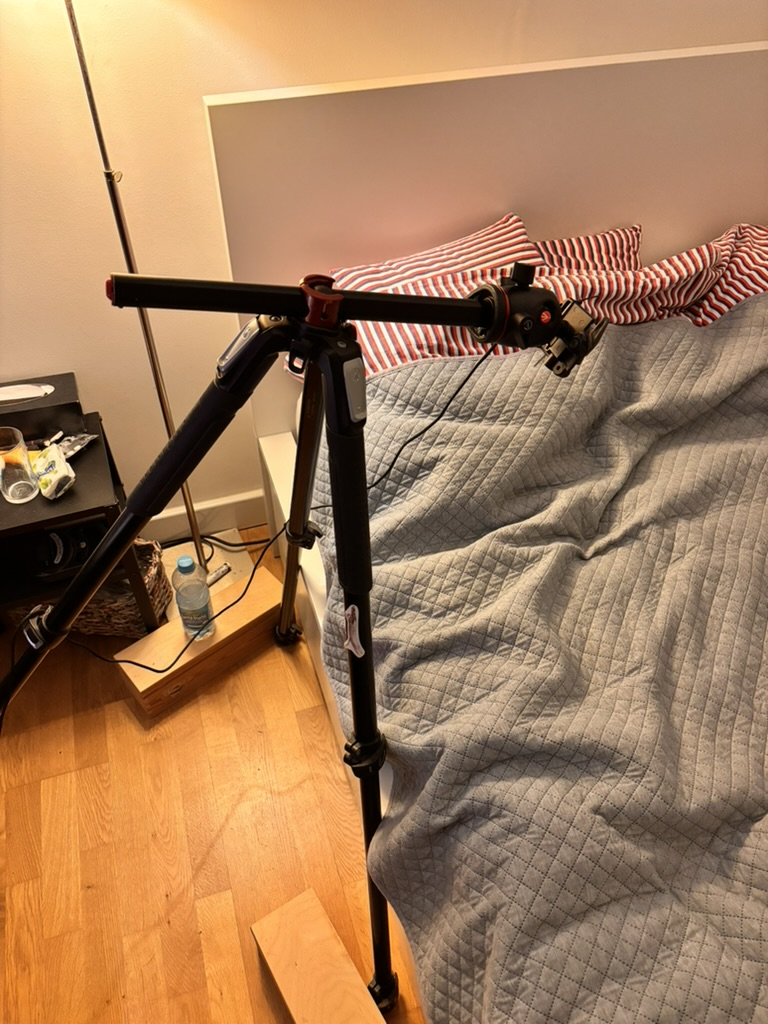
\includegraphics[width=0.56\textwidth]{stanowisko_a121_nad_lozkiem.jpg}
    \caption[Stanowisko A121 nad łóżkiem]{Stanowisko do pełnych pomiarów
    nocnych z~płaską pokrywą. Wysięgnik statywu wprowadza czujnik nad łóżko,
    a~regulowana głowica kieruje jego oś ukośnie na tułów. Na podstawie
    śledzonej bramki A121 efektywny dystans do dominującego celu wynosił
    około \SI{0.4}{m}.}
    \label{fig:stanowisko-sen}
\end{figure}

Osobno wykonano późniejszą noc z~soczewką hiperboliczną i~większego dystansu.
Mediana śledzonej odległości wynosiła \SI{1.62}{m}, lecz oś radaru była
odchylona od normalnej do klatki o~ponad \SI{60}{\degree}. Echo padało zatem
pod bardzo niekorzystnym kątem i~wynik oddechowy był niestabilny; nagranie
wyłączono z~porównania fizjologicznego. Nie jest to dowód ograniczenia
soczewki, tylko nieudanej geometrii stanowiska.

Czas ramek A121 zapisywano jako czas systemowy komputera, a~znaczniki FIT
przeliczano na tę samą strefę lokalną. Wartości Garmina przypisywano do okien
radaru metodą najbliższego znacznika z~tolerancją \SI{2}{min}. Nie była to
synchronizacja sprzętowa; wystarczała do trendów w~kroku \SI{30}{s}, lecz nie
pozwala analizować opóźnień pojedynczego uderzenia serca.

\section{Estymacja tętna i oddechu przez całą noc}
\label{sec:trend-nocny}
Algorytm z~rozdziału~\ref{chap:algorytmy} operuje na oknie kilkudziesięciu
sekund. Nocne nagranie trwa jednak 7--9~godzin i~zawiera długie okresy ruchu,
przewracania się oraz nieobecności. Analizę nocną realizuje więc nakładka
(\texttt{tools/\allowbreak analyze\_a121\_\allowbreak sleep\_vitals\_\allowbreak gated.py}), która przesuwa
\SI{60}{s} okno analizy z~krokiem \SI{30}{s} i~dla każdego okna wywołuje
analizator parametrów życiowych, budując trend HR/RR.

Kluczowe jest \textbf{bramkowanie okien}. Każdą ramkę klasyfikuje się na
podstawie stanu detektora obecności czujnika jako \emph{spoczynek}
(\texttt{still}), \emph{ruch} (\texttt{movement}) lub \emph{brak obecności}
(\texttt{no\_presence}). Dla okna liczy się frakcje tych stanów i~odrzuca
okno, gdy zachodzi którykolwiek z~warunków:
\begin{itemize}
  \item ostatnia ramka okna to ruch lub brak obecności (estymata byłaby
  publikowana w~momencie, gdy badanego już nie ma w~wiązce),
  \item frakcja braku obecności przekracza 0{,}05,
  \item okno zawiera ciągły ruch dłuższy niż \SI{30}{s},
  \item frakcja spoczynku spada poniżej 0{,}65.
\end{itemize}
Dodatkowo estymatę tętna przyjmuje się tylko przy pewności $\geq 5$
i~w~zakresie fizjologicznym \SIrange{42}{120}{ud\per\minute}. Krótkie przerwy
ruchowe (poniżej \SI{30}{s}) są sklejane, aby pojedyncze drgnięcie nie
rozbijało ciągłego odcinka snu na fragmenty.

Efektem jest szereg czasowy z~krokiem \SI{30}{s}, zawierający tętno, częstość
oddechu, frakcje stanów oraz dominujący stan okna --- to on jest wejściem
klasyfikatora faz snu. Duża część okien nocy jest odrzucana i~to jest
zachowanie pożądane: lepiej nie podać wartości niż podać wartość wziętą
z~artefaktu ruchowego.

\section{Algorytm klasyfikacji faz snu}
\label{sec:algorytm-snu}
Na podstawie trendu z~sekcji~\ref{sec:trend-nocny} zbudowano heurystyczny
klasyfikator faz snu (moduł \texttt{a121\_sleep}), rozróżniający czuwanie,
sen lekki, sen głęboki i~fazę REM. Nie jest to model uczony --- to zestaw
reguł opartych na znanych korelatach fizjologicznych, które \emph{są}
dostępne radarowi: tętno, oddech, ich zmienność oraz ruch ciała.

\paragraph{Cechy pochodne.} Z~trendu wyznacza się medianę kroczącą tętna
i~oddechu w~oknie \SI{5}{min} ($\overline{HR}$, $\overline{RR}$) oraz ich
odchylenie standardowe w~oknie \SI{10}{min} ($s_{HR}$, $s_{RR}$ --- miary
zmienności), a~także wygładzoną frakcję ruchu. Progi decyzyjne \emph{nie} są
stałymi bezwzględnymi, lecz percentylami wyznaczanymi \textbf{indywidualnie
dla danej nocy} --- inaczej klasyfikator nie przenosiłby się między osobami
ani między nocami:
\begin{itemize}
  \item $HR_{\text{deep}}$ --- mediana tętna podczas snu (percentyl~50),
  \item $s_{HR}^{70}$ --- percentyl~70 zmienności tętna,
  \item $s_{RR}^{60},\ s_{RR}^{75}$ --- percentyle 60 i~75 zmienności oddechu,
  \item $HR_{\text{base}}$, $\mathrm{IQR}_{HR}$ --- mediana i~rozstęp
  międzykwartylowy tętna podczas snu.
\end{itemize}

\paragraph{Wykrycie zaśnięcia i~przebudzenia.} Za moment zaśnięcia przyjmuje
się początek pierwszego okresu, w~którym przez kolejne \SI{30}{min} utrzymuje
się (w~co najmniej 80\% okien) spoczynek: frakcja spoczynku $\geq 0{,}80$,
frakcja ruchu $\leq 0{,}20$, brak obecności $\leq 0{,}05$ oraz dostępna
estymata tętna lub oddechu. Jeżeli wewnątrz tego okresu wystąpi jeszcze silny
ruch, zaśnięcie przesuwa się za jego koniec. Przebudzenie wykrywa się tylko
wtedy, gdy nagranie kończy się co najmniej \SI{20}{min} ciągłym okresem
ruchu/nieobecności; w~przeciwnym razie za moment wybudzenia przyjmuje się
koniec nagrania --- to jedyna uczciwa interpretacja, bo radar nie ma innej
przesłanki, że badany wstał.

\paragraph{Reguły decyzyjne.} Dla każdego okna wewnątrz okresu snu:
\begin{itemize}
  \item \textbf{Czuwanie} (arousal): frakcja braku obecności $> 0{,}20$ lub
  frakcja ruchu $> 0{,}35$, albo stan okna wskazuje ruch/nieobecność.
  \item \textbf{Sen głęboki}: co najmniej \SI{20}{min} od zaśnięcia, ruch
  $< 0{,}10$, tętno $\overline{HR} \leq HR_{\text{deep}}$ (poniżej mediany
  nocnej), niska zmienność oddechu $s_{RR} \leq s_{RR}^{60}$ oraz pierwsze
  70\% nocy. Odzwierciedla to fizjologię: w~śnie wolnofalowym tętno spada,
  a~oddech staje się regularny; sen głęboki koncentruje się w~pierwszej
  połowie nocy.
  \item \textbf{REM}: co najmniej \SI{75}{min} od zaśnięcia i~po 18\% nocy,
  mały ruch ($< 0{,}15$), ale \emph{podwyższona zmienność} --- $s_{HR} \geq
  s_{HR}^{70}$ lub $s_{RR} \geq s_{RR}^{75}$. W~REM występuje atonia mięśni
  (ciało nieruchome), lecz oddech i~tętno stają się nieregularne; to właśnie
  ta kombinacja odróżnia REM od snu głębokiego, w~którym ciało również jest
  nieruchome.
  \item \textbf{Sen lekki} --- przypadek domyślny.
\end{itemize}
Gdy reguły snu głębokiego i~REM zostaną spełnione jednocześnie, w~drugiej
połowie nocy (po 55\% czasu snu) pierwszeństwo ma REM.

\paragraph{Postprzetwarzanie.} Krótkie ,,wysepki'' faz nie-czuwania krótsze
niż \SI{4}{min} są scalane z~otoczeniem, aby hipnogram był czytelny; epizody
czuwania \emph{nie} są scalane --- usunięcie ich zatarłoby dowody wybudzeń.
Pierwsza wersja reguł dopuszczała również bezpośrednie przejścia
REM~$\leftrightarrow$~sen głęboki. Ponieważ przy rozdzielczości
\SI{30}{s} bezpieczniejszą interpretacją jest przejście przez lżejsze stadium,
do wersji końcowej dodano jawne ograniczenie strukturalne: pierwsze
\SI{4}{min} fazy docelowej po takim skoku oznacza się jako sen lekki. Korekta
nie korzysta z~etykiet Garmina ani nie zmienia progów HR/RR; każde zmienione
okno zachowuje osobną flagę
\texttt{radar\_direct\_transition\_bridge\_to\_light} i~jest zaznaczone na
hipnogramach jasnym żółtym tłem.
Osobno wykryto specyficzny przypadek: \emph{spokojne, ale pofragmentowane
leżenie nad ranem} (np. leżenie w~łóżku z~telefonem po głównym epizodzie snu).
Mały ruch ciała imituje wtedy REM, dlatego w~ostatnich 12\% okresu snu, jeśli
utrzymuje się wysoka nieruchomość przy powtarzających się drobnych sygnałach
ruchu, kandydaci REM są degradowani do snu lekkiego.

\paragraph{Status wyniku: estymacja, nie pomiar.} Należy zaznaczyć
wprost: \textbf{wyznaczonych faz snu nie da się w~tej pracy zweryfikować}.
Jedynym dostępnym odniesieniem był zegarek Garmin~Fenix~7, a~on \emph{sam
również nie jest metodą referencyjną} --- to urządzenie konsumenckie, które
fazy snu szacuje heurystycznie z~tętna, HRV, ruchu i~(w~nowszych modelach)
pulsoksymetrii. Złotym standardem pozostaje polisomnografia (EEG, EOG, EMG),
której w~tym projekcie nie było. Rozbieżność radar--Garmin \emph{nie dowodzi
zatem błędu radaru}: mówi tylko tyle, że dwie heurystyki oparte na sygnałach
zastępczych dały różne wyniki, i~z~samego porównania nie wynika, która z~nich
jest bliżej prawdy. Ani sen głęboki, ani REM nie są przez ten system
\emph{mierzone} --- są \emph{estymowane} regułami zebranymi wyżej, opartymi na
znanych korelatach fizjologicznych (spadek i~stabilizacja tętna w~śnie
wolnofalowym, wzrost nieregularności tętna i~oddechu przy atonii mięśniowej
w~REM). Wszystkie liczby dotyczące faz snu w~dalszej części należy czytać
z~tym zastrzeżeniem.

\miejsce{Miejsce na przegląd literatury o~dokładności faz snu w~urządzeniach
konsumenckich: badania walidacyjne Garmina (i~pokrewnych: Fitbit, Oura,
Withings) względem polisomnografii --- typowo wysoka czułość detekcji \emph{snu
jako takiego} (rzędu 0,9), ale znacznie słabsza zgodność \emph{stadiów},
w~szczególności notoryczne mylenie snu głębokiego z~lekkim i~zawyżanie/zaniżanie
REM; podać raportowane wartości $\kappa$ Cohena i~dokładność 4-klasową. To jest
uzasadnienie, dlaczego Garmin jest w~tej pracy traktowany jako \emph{punkt
odniesienia}, a~nie jako \emph{prawda}.}

\section{Ocena jakości snu (\emph{sleep score})}
\label{sec:sleep-score}

\paragraph{Charakter metryki.} Należy rozpocząć od zastrzeżenia rzadko
obecnego w~materiałach producentów: \emph{ocena snu} (\emph{sleep
score}) w~skali 0--100 jest metryką zdefiniowaną przez producentów
urządzeń, a~nie wielkością fizjologiczną ani kliniczną. Nie odpowiada jej
żadna jednostka, żadne badanie referencyjne ani żadna definicja w~medycynie snu
--- polisomnografia nie zwraca wartości w~tej skali. Każdy producent (Garmin, Fitbit,
Oura, Withings) wyznacza ją inaczej i~z~innych składowych, a~konkretne wzory są
tajemnicą handlową; ta sama noc oceniona dwoma urządzeniami może dać
istotnie różne wyniki. Rozpatrywana samodzielnie liczba ta nie niesie
znaczenia bezwzględnego --- jest co najwyżej wskaźnikiem zbiorczym, który agreguje
kilka mierzalnych cech nocy
(długość, ciągłość, proporcje faz, spokój, parametry witalne) w~jedną wartość
porównywalną przede wszystkim między kolejnymi nocami tego samego urządzenia.

Mimo to metryka ta jest powszechnie oczekiwana przez użytkownika, dlatego
--- wyłącznie ze względu na jej popularność i~porównywalność z~zegarkiem
konsumenckim --- opracowano algorytm, który w~przybliżeniu odtwarza
zachowanie oceny Garmina. Odtworzono \emph{zachowanie}, nie wzór: wzór Garmina
nie jest publiczny. Charakterystyczne dla ocen konsumenckich (i~odtworzone
tutaj) są dwie cechy: dominująca rola długości snu oraz nasycanie się składowych
--- wartość cechy uznana za wystarczającą daje komplet punktów, a~pogorszenie
karane jest liniowo.

\paragraph{Konstrukcja.} Ocena jest sumą pięciu składowych, ograniczoną z~góry
pułapem zależnym od całkowitego czasu snu $T$ (w~minutach):
\begin{equation}
  \mathrm{score} = \min\big(D + C + B + R + V,\ \mathrm{cap}(T)\big),
  \qquad D+C+B+R+V \leq 100 .
  \label{eq:sleep-score}
\end{equation}
Wszystkie składowe zbudowano z~funkcji nasycającej
$\sigma(x) = \min(\max(x,0),1)$ (obcięcie do przedziału $[0,1]$), co gwarantuje
ograniczoność i~monotoniczność każdego członu:
\begin{align}
  D &= 30\,\sigma\!\left(\frac{T}{480}\right) \cdot
       \begin{cases}
         1, & T \leq 540,\\[2pt]
         \sigma\!\left(1 - \dfrac{T-540}{180}\right), & T > 540,
       \end{cases}
       \label{eq:score-d}\\[2pt]
  C &= 15\,\sigma\!\left(\frac{\eta - 0{,}75}{0{,}18}\right)
     + 3\,\sigma\!\left(1 - \frac{T_{\text{awake}}}{60}\right)
     + 2\,\sigma\!\left(1 - \frac{n_{\text{aw}}}{4}\right),
       \label{eq:score-c}\\[2pt]
  B &= 10\,Q(p_{\text{deep}};\,4,13,23,33\,\%)
     + 10\,Q(p_{\text{rem}};\,8,18,27,40\,\%),
       \label{eq:score-b}\\[2pt]
  R &= 8\,\sigma\!\left(1 - \frac{\overline{m}}{0{,}08}\right)
     + 3\,\sigma\!\left(1 - \frac{\overline{u}}{0{,}03}\right)
     + 4\,\sigma\!\left(1 - \frac{n_{\text{aw}}}{6}\right),
       \label{eq:score-r}\\[2pt]
  V &= 7\,\sigma\!\left(1 - \frac{[\widetilde{HR} - 55]_+}{25}\right)
     + 4\,\sigma\!\left(1 - \frac{[s_{HR} - 4]_+}{8}\right)
     + 4\,\sigma\!\left(1 - \frac{[s_{RR} - 1{,}2]_+}{3}\right),
       \label{eq:score-v}
\end{align}
gdzie $\eta$ --- efektywność snu (sen/okres snu), $T_{\text{awake}}$ --- minuty
czuwania, $n_{\text{aw}}$ --- liczba wybudzeń dłuższych niż \SI{1}{min}
na~godzinę, $\overline{m}$, $\overline{u}$ --- średnia frakcja ruchu
i~nieobecności, $\widetilde{HR}$ --- mediana tętna we śnie, $s_{HR}$, $s_{RR}$
--- odchylenia standardowe tętna i~oddechu, $[x]_+ = \max(x,0)$, a~$p_{\text{deep}}$,
$p_{\text{rem}}$ --- procentowe udziały faz. Sens progów jest następujący:
pełne \num{30} punktów za długość otrzymuje się dopiero przy \SI{8}{h} snu
(kara zaczyna się powyżej \SI{9}{h}); efektywność \SI{93}{\%} wysyca składową
ciągłości; mediana tętna do 55~bpm i~odchylenie tętna do 4~bpm dają komplet
punktów za regenerację.

Proporcje faz ocenia funkcja plateau $Q$ --- trapez, który daje maksimum
w~przedziale uznawanym za prawidłowy i~maleje liniowo \emph{po obu stronach},
karząc zarówno niedobór, jak i~nadmiar danej fazy:
\begin{equation}
  Q(p;\,a,b,c,d) =
  \begin{cases}
    0, & p \leq a \ \text{lub}\ p \geq d,\\[2pt]
    \dfrac{p-a}{b-a}, & a < p < b,\\[4pt]
    1, & b \leq p \leq c,\\[4pt]
    \dfrac{d-p}{d-c}, & c < p < d .
  \end{cases}
  \label{eq:plateau}
\end{equation}
Dla snu głębokiego plateau przyjęto na 13--23\%, dla REM na 18--27\% czasu snu.

Kluczowy jest jednak nie sam wzór, lecz \emph{pułap} $\mathrm{cap}(T)$, bo to on
--- podobnie jak w~zegarkach konsumenckich --- w~praktyce decyduje o~ocenie:
\begin{equation}
  \mathrm{cap}(T) =
  \begin{cases}
    30 + 30\,\sigma\!\left(\frac{T}{240}\right), & T < \SI{240}{min}\ (\SI{4}{h}),\\[4pt]
    60 + 20\,\sigma\!\left(\frac{T-240}{180}\right), & \SI{240}{min} \leq T < \SI{420}{min}\ (\SI{7}{h}),\\[4pt]
    80 + 20\,\sigma\!\left(\frac{T-420}{60}\right), & \SI{420}{min} \leq T < \SI{480}{min},\\[4pt]
    100, & T \geq \SI{480}{min}\ (\SI{8}{h}).
  \end{cases}
  \label{eq:duration-cap}
\end{equation}
Krótka noc \emph{nie może} więc zostać oceniona wysoko, choćby była idealnie
spokojna i~ciągła --- poniżej \SI{4}{h} snu maksimum to 60~punktów. Widać to
w~zebranych danych: dla wszystkich analizowanych nocy suma składowych
($\mathrm{raw\ score}$) była wyższa od oceny końcowej, a~ograniczał ją właśnie
pułap czasu (np. noc~1: składowe 83,8~pkt, pułap 73,8~pkt $\rightarrow$ ocena
74). Innymi słowy: \emph{ocena zależy przede wszystkim od długości snu}, a~pozostałe
składowe jedynie ją modulują --- co odpowiada zarazem sposobowi działania
ocen snu w~urządzeniach komercyjnych.

\begin{table}[H]
\centering
\caption[Składowe oceny jakości snu]{Składowe punktowej oceny snu
(\texttt{score\_radar\_sleep}). Maksimum sumy wynosi 100~punktów, a~dodatkowo
całość ogranicza pułap zależny od długości snu, wzór~\eqref{eq:duration-cap}.}
\label{tab:sleep-score}
\small
\begin{tabular}{@{}llr@{}}
\toprule
\textbf{Składowa} & \textbf{Co ocenia} & \textbf{Maks.} \\
\midrule
Długość $D$        & czas snu względem \SI{8}{h}; kara za sen $>\SI{9}{h}$ & 30 \\
Ciągłość $C$       & efektywność snu, minuty czuwania, liczba wybudzeń/h & 20 \\
Proporcje faz $B$  & udział snu głębokiego (13--23\%) i~REM (18--27\%) & 20 \\
Spokój $R$         & średnia frakcja ruchu i~nieobecności, wybudzenia & 15 \\
Regeneracja $V$    & mediana tętna, stabilność tętna i~oddechu & 15 \\
\bottomrule
\end{tabular}
\end{table}

Etykieta słowna przypisywana jest progowo: $\geq 90$ --- ,,doskonała'',
$\geq 80$ --- ,,dobra'', $\geq 60$ --- ,,przeciętna'', poniżej --- ,,słaba''.
Tętno spoczynkowe szacuje się jako 10.~percentyl tętna w~oknach snu o~znikomym
ruchu.

\paragraph{Zgodność oceny z~eksportem Garmin~Connect.} Dla nocy~1 udało się
odzyskać pełny eksport oceny z~aplikacji Garmin~Connect (\texttt{Sleep.csv}),
co pozwala zestawić obie metryki bezpośrednio (tab.~\ref{tab:score-garmin}).
Zgodność samej oceny jest wysoka: \textbf{74~punkty w~obu przypadkach}
i~identyczna etykieta jakości, przy niezależnie wyznaczonym czasie snu
różniącym się o~7~minut. Zgodne jest również tętno spoczynkowe --- \SI{52.7}{bpm}
z~radaru wobec \SI{51}{bpm} z~zegarka --- co potwierdza działanie opisanego
wcześniej estymatora tętna spoczynkowego.

\begin{table}[H]
\centering
\caption[Ocena snu i fazy: radar a dwa eksporty Garmina (noc 1)]{Noc~1 ---
zestawienie wyniku własnego z~\emph{dwoma} źródłami danych z~tego samego
zegarka: surowym strumieniem \texttt{SLEEP\_DATA} z~pliku FIT (to jego użyto
w~tab.~\ref{tab:fazy}) oraz podsumowaniem pokazywanym użytkownikowi
w~aplikacji Garmin~Connect. Oba pochodzą z~tej samej nocy i~tego samego
urządzenia.}
\label{tab:score-garmin}
\small
\begin{tabular}{@{}lrrr@{}}
\toprule
 & \textbf{Radar} & \textbf{Garmin} & \textbf{Garmin} \\
 & \textbf{(ta praca)} & \textbf{(FIT)} & \textbf{(Connect)} \\
\midrule
Ocena snu [pkt]        & 74 & --- & 74 \\
Etykieta jakości       & \emph{Fair} & --- & \emph{Fair} \\
Czas snu [min]         & 364,5 & 326,0 & 357,0 \\
Sen głęboki [min]      & 70,5 & 57,0 & 82,0 \\
Sen lekki [min]        & 224,5 & 222,0 & 159,0 \\
REM [min]              & 69,5 & 47,0 & 116,0 \\
Czuwanie [min]         & 24,0 & 40,0 & 24,0 \\
\midrule
Sen głęboki [\% snu]   & 19,3 & 17,5 & 23,0 \\
REM [\% snu]           & 19,1 & 14,4 & 32,5 \\
\midrule
Tętno spoczynkowe [bpm] & 52,7 & --- & 51 \\
\bottomrule
\end{tabular}
\end{table}

\paragraph{Rozbieżność dwóch eksportów tego samego zegarka.}
Tabela~\ref{tab:score-garmin} wskazuje jednak obserwację ważniejszą w~tej pracy
niż sama zgodność oceny:
\textbf{dwa eksporty z~tego samego zegarka, dotyczące tej samej nocy, podają
istotnie różne fazy snu}. Surowy strumień FIT przypisuje REM 47~minut,
a~aplikacja --- 116~minut; sen głęboki odpowiednio 57 i~82~minuty. Różnica
w~REM jest \emph{dwuipółkrotna}. Nie jest to błąd odczytu: strumień
\texttt{SLEEP\_DATA} zawiera znaczniki zmian stadium rejestrowane na
urządzeniu, a~aplikacja pokazuje wynik po własnym (niejawnym)
postprzetwarzaniu w~chmurze.

Prowadzi to do wniosku, że Garmina nie można traktować jako wzorca, skoro
dwa jego własne eksporty nie są ze sobą zgodne. Zależnie od tego, który eksport
przyjmiemy za odniesienie, radar raz \emph{zawyża} sen głęboki (o~13,5~min względem FIT),
a~raz \emph{zaniża} (o~11,5~min względem aplikacji) --- przy dokładnie tych
samych danych radarowych. Jest to istotny argument za
tym, że rozbieżności faz snu z~sekcji~\ref{sec:fazy-wyniki} nie należy
interpretować jako błędu radaru.

Sama zgodność oceny (74 wobec 74) również nie jest dowodem poprawności; warto
przy tym wyjaśnić, \emph{dlaczego} okazała się tak wysoka. Ocena jest zdominowana przez czas
snu (wzór~\eqref{eq:duration-cap}), a~czas snu obie metody mierzą podobnie, bo
obie wykrywają to samo: brak ruchu i~spadek tętna. Rozbieżność ujawnia się dopiero
tam, gdzie czas snu nie jest rozstrzygający --- w~proporcjach faz. \textbf{Zgodne oceny
przy niezgodnych fazach} ilustrują tezę tej sekcji: ocena snu
jest agregatem o~małej rozdzielczości informacyjnej. Pojedyncza noc stanowi
przy tym obserwację jednostkową, a~nie walidację.

\todo{Uzasadnić progi literaturowo (odsetki faz snu u~dorosłych). Rozważyć
krótki przegląd: jak liczą ocenę snu Garmin/Fitbit/Oura i~dlaczego wyniki nie
są porównywalne między producentami. Podsumowanie \texttt{Sleep.csv}
z~Garmin~Connect udało się odzyskać tylko dla nocy~1 --- dla
pozostałych nocy głównego porównania warto je dociągnąć i~powtórzyć
tabelę~\ref{tab:score-garmin}, aby sprawdzić, czy rozbieżność FIT~vs~Connect
powtarza się co noc. Surowe eksporty FIT dla nocy~1--3 są dostępne.}

\section{Wyniki: podsumowanie radarowe}

\begin{table}[H]
\centering
\caption{Podsumowanie snu wyznaczone wyłącznie z~radaru. Pierwsze trzy
wiersze tworzą główny zestaw porównawczy z~eksportem Garmina; dwa ostatnie
pokazują powtarzalność stanowiska z~płaską pokrywą nad łóżkiem.}
\label{tab:sensummary}
\small
\resizebox{\textwidth}{!}{%
\begin{tabular}{@{}lrrrrl@{}}
\toprule
Nagranie / konfiguracja & Ocena & Sen całk. [min] & Efektywność [\%] & Spocz. HR [bpm] & Jakość \\
\midrule
Noc 1 (plano-convex, krawędź) & 74 & 364,5 & 93,8 & 52,7 & Przeciętna \\
Noc 2 (FZP, krawędź)          & 71 & 342,5 & 95,0 & 51,9 & Przeciętna \\
Noc 3 (płaska, nad łóżkiem)   & 93 & 485,0 & 97,1 & 49,7 & Doskonała \\
Noc 4 (płaska, nad łóżkiem)   & 78 & 454,5 & 89,4 & 51,1 & Przeciętna \\
Noc 5 (płaska, nad łóżkiem)   & 91 & 551,0 & 97,6 & 50,5 & Doskonała \\
\bottomrule
\end{tabular}%
}
\end{table}

Wszystkie pokazane zapisy są pełnymi nocami. Oszacowane tętno spoczynkowe
pozostało spójne (około 50--53~bpm), a~trzy noce z~płaską pokrywą pokazują,
że stanowisko nad łóżkiem może powtarzalnie dostarczać wielogodzinne trendy.
Wyższej oceny nocy~3 nie należy jednak utożsamiać z~walidacją faz:
punktowa metryka silnie zależy od długości i~ciągłości zapisu.

\section{Wyniki: jakość techniczna trzech konfiguracji}

Ponieważ surowa amplituda może pochodzić od krawędzi łóżka, porównanie
konfiguracji oparto również na odsetku okien zaakceptowanych przez bramkowanie,
dostępności HR/RR oraz błędzie bezwzględnym względem równoległego trendu
Garmina. Tabela~\ref{tab:sen-jakosc} dotyczy trzech pełnych nocy głównego
porównania.

\begin{table}[H]
\centering
\caption{Techniczna użyteczność trendów dla trzech pełnych nocy. ,,Ważne
okna'' oznaczają status \texttt{valid}, dostępność HR/RR dotyczy
nieinterpolowanych estymat, a~MAE jest średnim błędem bezwzględnym
w~sparowanych oknach snu.}
\label{tab:sen-jakosc}
\small
\resizebox{\textwidth}{!}{%
\begin{tabular}{@{}lrrrrr@{}}
\toprule
Konfiguracja & Ważne okna [\%] & HR dostępne [\%] &
RR dostępne [\%] & HR MAE [bpm] & RR MAE [odd./min] \\
\midrule
Noc 1, plano-convex przy krawędzi & 89,9 & 70,5 & 89,9 & 3,9 & 2,0 \\
Noc 2, FZP przy krawędzi          & 91,8 & 80,8 & 91,8 & 3,9 & 1,6 \\
Noc 3, płaska nad łóżkiem         & 94,5 & 77,6 & 94,5 & 3,8 & 1,3 \\
\bottomrule
\end{tabular}%
}
\end{table}

Ustawienie z~płaską pokrywą uzyskało największy udział zaakceptowanych okien
i~najmniejszy MAE oddechu. Dostępność tętna była natomiast największa dla FZP,
a~różnica HR MAE między konfiguracjami jest mała. Wynik nie pozwala więc
stwierdzić, że płaska pokrywa jest lepszą anteną; pokazuje, że kompletne
stanowisko \emph{płaska pokrywa + wysięgnik nad tułowiem} było bardziej
użyteczne niż dwa początkowe stanowiska przy krawędzi.

\section{Wyniki: porównanie tętna z Garmin Fenix 7}

\begin{table}[H]
\centering
\caption{Porównanie tętna (okna snu): radar vs Garmin Fenix~7.}
\label{tab:hr}
\small
\resizebox{\textwidth}{!}{%
\begin{tabular}{@{}lrrrr@{}}
\toprule
Noc & Radar śr. [bpm] & Garmin śr. [bpm] & Obciążenie śr. & Obciążenie med. \\
\midrule
Noc 1 (plano-convex, krawędź) & 55,5 & 57,4 & $-1{,}9$ & $-1{,}8$ \\
Noc 2 (FZP, krawędź)          & 55,1 & 58,3 & $-3{,}3$ & $-2{,}4$ \\
Noc 3 (płaska, nad łóżkiem)   & 52,5 & 52,7 & $-0{,}1$ & $+0{,}4$ \\
\bottomrule
\end{tabular}%
}
\end{table}

Zgodność tętna jest najważniejszym wynikiem praktycznym, ponieważ --- w~
przeciwieństwie do surowej amplitudy --- jest odporna na problem odbicia od
krawędzi łóżka. Noc z~płaską pokrywą miała najmniejsze średnie obciążenie HR
($-0{,}1$~bpm), podczas gdy ustawienia przy krawędzi zaniżały tętno średnio
o~\SI{1.9}{bpm} i~\SI{3.3}{bpm}. Nie dowodzi to wyższości płaskiej pokrywy,
pokazuje natomiast, że przewaga w~zysku anteny nie przekłada się
automatycznie na lepszą zgodność fizjologiczną w~danym ustawieniu. Wiarygodną
hipotezą wyjaśniającą jest geometria pomiaru: soczewki skupiające zawężają
obszar obserwacji, więc zmiana pozycji śpiącej osoby lub niedokładne utrzymanie
osi radaru na klatce może usunąć właściwy reflektor z~głównej wiązki. Płaska
pokrywa obejmuje szerszy obszar i~przy małych odległościach może być bardziej
odporna na takie przesunięcie, mimo mniejszego zysku. Ponieważ każdy wariant
soczewki badano innej nocy, zebrane dane nie pozwalają oddzielić wpływu
soczewki od wpływu ułożenia ciała i~mocowania; jest to interpretacja, a~nie
wykazany związek przyczynowy. Dla nocy~4 i~5 eksport zegarka nie
był dostępny, dlatego
nie dopisano im pozornej ,,referencji'' i~pokazano jedynie przebiegi radarowe.

\section{Wyniki: porównanie częstości oddechu}

\begin{table}[H]
\centering
\caption{Porównanie częstości oddechu (okna snu): radar vs Garmin Fenix~7.}
\label{tab:rr}
\small
\resizebox{\textwidth}{!}{%
\begin{tabular}{@{}lrrrr@{}}
\toprule
Noc & Radar śr. [odd./min] & Garmin śr. & Obciążenie śr. & Obciążenie med. \\
\midrule
Noc 1 (plano-convex, krawędź) & 13,6 & 14,0 & $-0{,}4$ & $-0{,}2$ \\
Noc 2 (FZP, krawędź)          & 14,6 & 14,2 & $+0{,}4$ & $+0{,}5$ \\
Noc 3 (płaska, nad łóżkiem)   & 14,5 & 13,7 & $+0{,}7$ & $+0{,}6$ \\
\bottomrule
\end{tabular}%
}
\end{table}

Średnie obciążenie częstości oddechu nie przekroczyło
0{,}7~oddechu/min w~żadnej z~trzech pełnych nocy. Ustawienie
z~płaską pokrywą miało nieco większe obciążenie średnie, ale najmniejszy MAE
okienny (tab.~\ref{tab:sen-jakosc}), dlatego pojedyncza średnia nie powinna
zastępować oceny całego przebiegu. Nadal jest to porównanie z~urządzeniem
konsumenckim, a~nie walidacja kliniczna.

\section{Wyniki: porównanie faz snu}
\label{sec:fazy-wyniki}

Zgodnie z~zastrzeżeniem z~sekcji~\ref{sec:algorytm-snu}: poniższe zestawienie
jest \emph{porównaniem dwóch estymat}, a~nie oceną dokładności względem prawdy.
Garmin nie jest tu wzorcem --- fazy snu szacuje własną, niejawną heurystyką,
której zgodność ze stadiami polisomnograficznymi jest w~literaturze umiarkowana.
Różnica ,,radar $-$ Garmin'' mierzy więc rozbieżność dwóch przybliżeń.

\begin{table}[H]
\centering
\caption{Sumaryczny czas trwania faz snu. Różnica dodatnia oznacza, że radar
przypisał danej fazie więcej czasu niż Garmin. Obie kolumny są estymatami ---
żadna z~nich nie jest odniesieniem polisomnograficznym.}
\label{tab:fazy}
\small
\begin{tabular}{@{}llrrrr@{}}
\toprule
Noc & Źródło & Czuwanie & Sen lekki & Sen głęboki & REM \\
 & & [min] & [min] & [min] & [min] \\
\midrule
Noc 1 & Radar    & 24,0 & 224,5 & 70,5 & 69,5 \\
Noc 1 & Garmin   & 40,0 & 222,0 & 57,0 & 47,0 \\
Noc 1 & Różnica  & $-16{,}0$ & $+2{,}5$ & $+13{,}5$ & $+22{,}5$ \\
\midrule
Noc 2 & Radar    & 18,0 & 207,0 & 50,0 & 85,5 \\
Noc 2 & Garmin   & 5,0  & 211,0 & 18,0 & 117,0 \\
Noc 2 & Różnica  & $+13{,}0$ & $-4{,}0$ & $+32{,}0$ & $-31{,}5$ \\
\midrule
Noc 3 & Radar   & 14,5 & 245,5 & 120,5 & 119,0 \\
Noc 3 & Garmin  & 51,0 & 284,0 & 31,0  & 115,0 \\
Noc 3 & Różnica & $-36{,}5$ & $-38{,}5$ & $+89{,}5$ & $+4{,}0$ \\
\bottomrule
\end{tabular}
\end{table}

Względem strumienia FIT radar przypisywał więcej czasu fazie snu głębokiego
we wszystkich trzech nocach (o~13,5, 32 i~89,5~minuty). Największa rozbieżność
wystąpiła właśnie w~nocy~3, mimo dobrej ciągłości HR/RR. Pokazuje to, że
stabilny pomiar parametrów życiowych nie jest równoznaczny z~poprawnym
rozpoznaniem stadiów. Wniosek trzeba dodatkowo osłabić: jak
pokazano w~tabeli~\ref{tab:score-garmin}, \emph{drugi} eksport z~tego samego
zegarka (podsumowanie z~aplikacji Garmin~Connect) podaje dla nocy~1 sen głęboki
82~minuty --- czyli \emph{więcej} niż radar (70,5~min). Kierunek rozbieżności
odwraca się więc w~zależności od tego, który eksport Garmina uzna się za
odniesienie, przy niezmienionych danych radarowych. Ostrożna konkluzja brzmi:
radar i~Garmin różnią się w~proporcjach faz, ale dane nie pozwalają orzec,
która heurystyka jest bliżej rzeczywistości.

Istotna obserwacja diagnostyczna dotyczyła \emph{struktury} hipnogramu.
Pierwsza wersja klasyfikatora dopuszczała w~analizowanych nocach bezpośrednie
przejścia REM~$\leftrightarrow$~sen głęboki. Zamiast dostrajać progi do
zegarka, wprowadzono opisany wcześniej, niezależny od Garmina warunek przejścia
przez sen lekki. W~wyniku końcowym
bezpośrednich przejść REM~$\leftrightarrow$~sen głęboki już nie ma; w~nocach~1,
2 i~3 przeniesiono do snu lekkiego odpowiednio 12, 16 i~28~minut.
Jest to naprawa niespójności reguł, nie dowód poprawności pozostałych etykiet.

\begin{figure}[p]
    \centering
    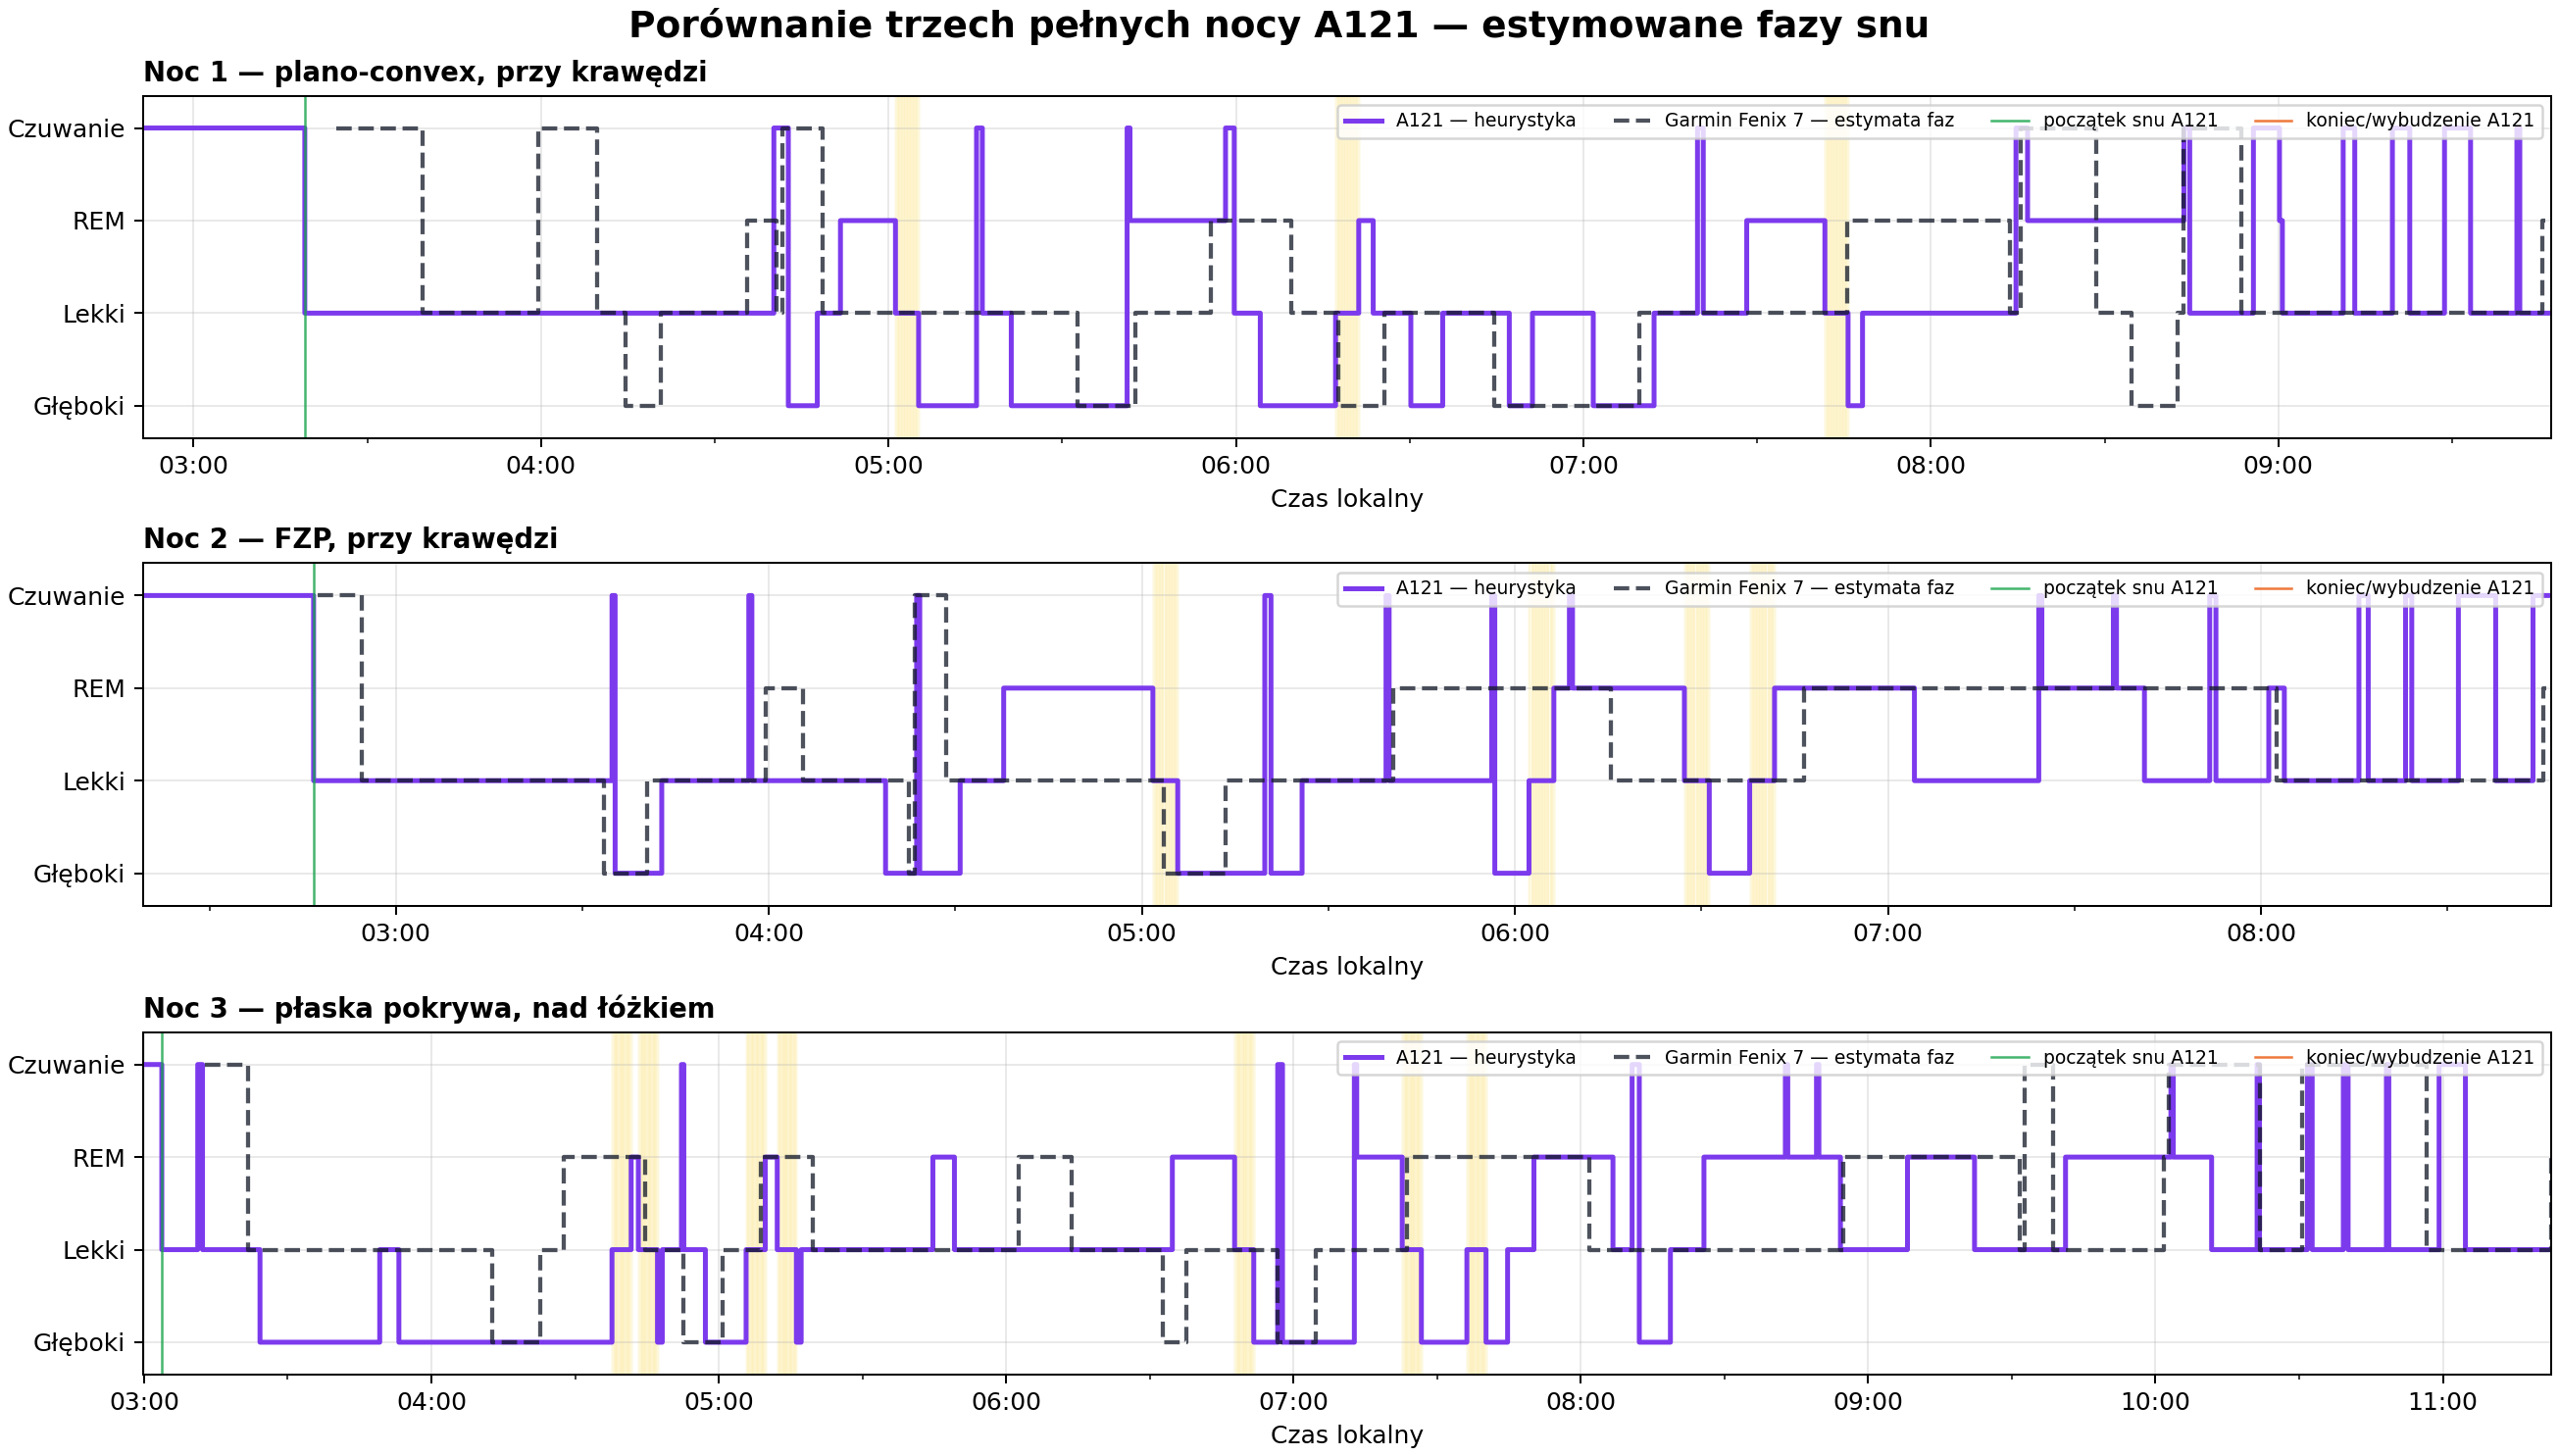
\includegraphics[width=\textwidth]{sen_porownanie_konfiguracji_fazy.png}
    \caption[Fazy snu w trzech pełnych nocach]{Estymowane fazy snu dla
    plano-convex przy krawędzi, FZP przy krawędzi i~płaskiej pokrywy nad
    łóżkiem. Dla wszystkich trzech nocy dostępny jest eksport Garmina. Linia
    fioletowa oznacza wynik A121, przerywana --- estymatę Garmina, a~jasne
    żółte pola --- okna skorygowane regułą przejścia przez sen lekki.}
    \label{fig:sen-porownanie-fazy}
\end{figure}

\begin{figure}[p]
    \centering
    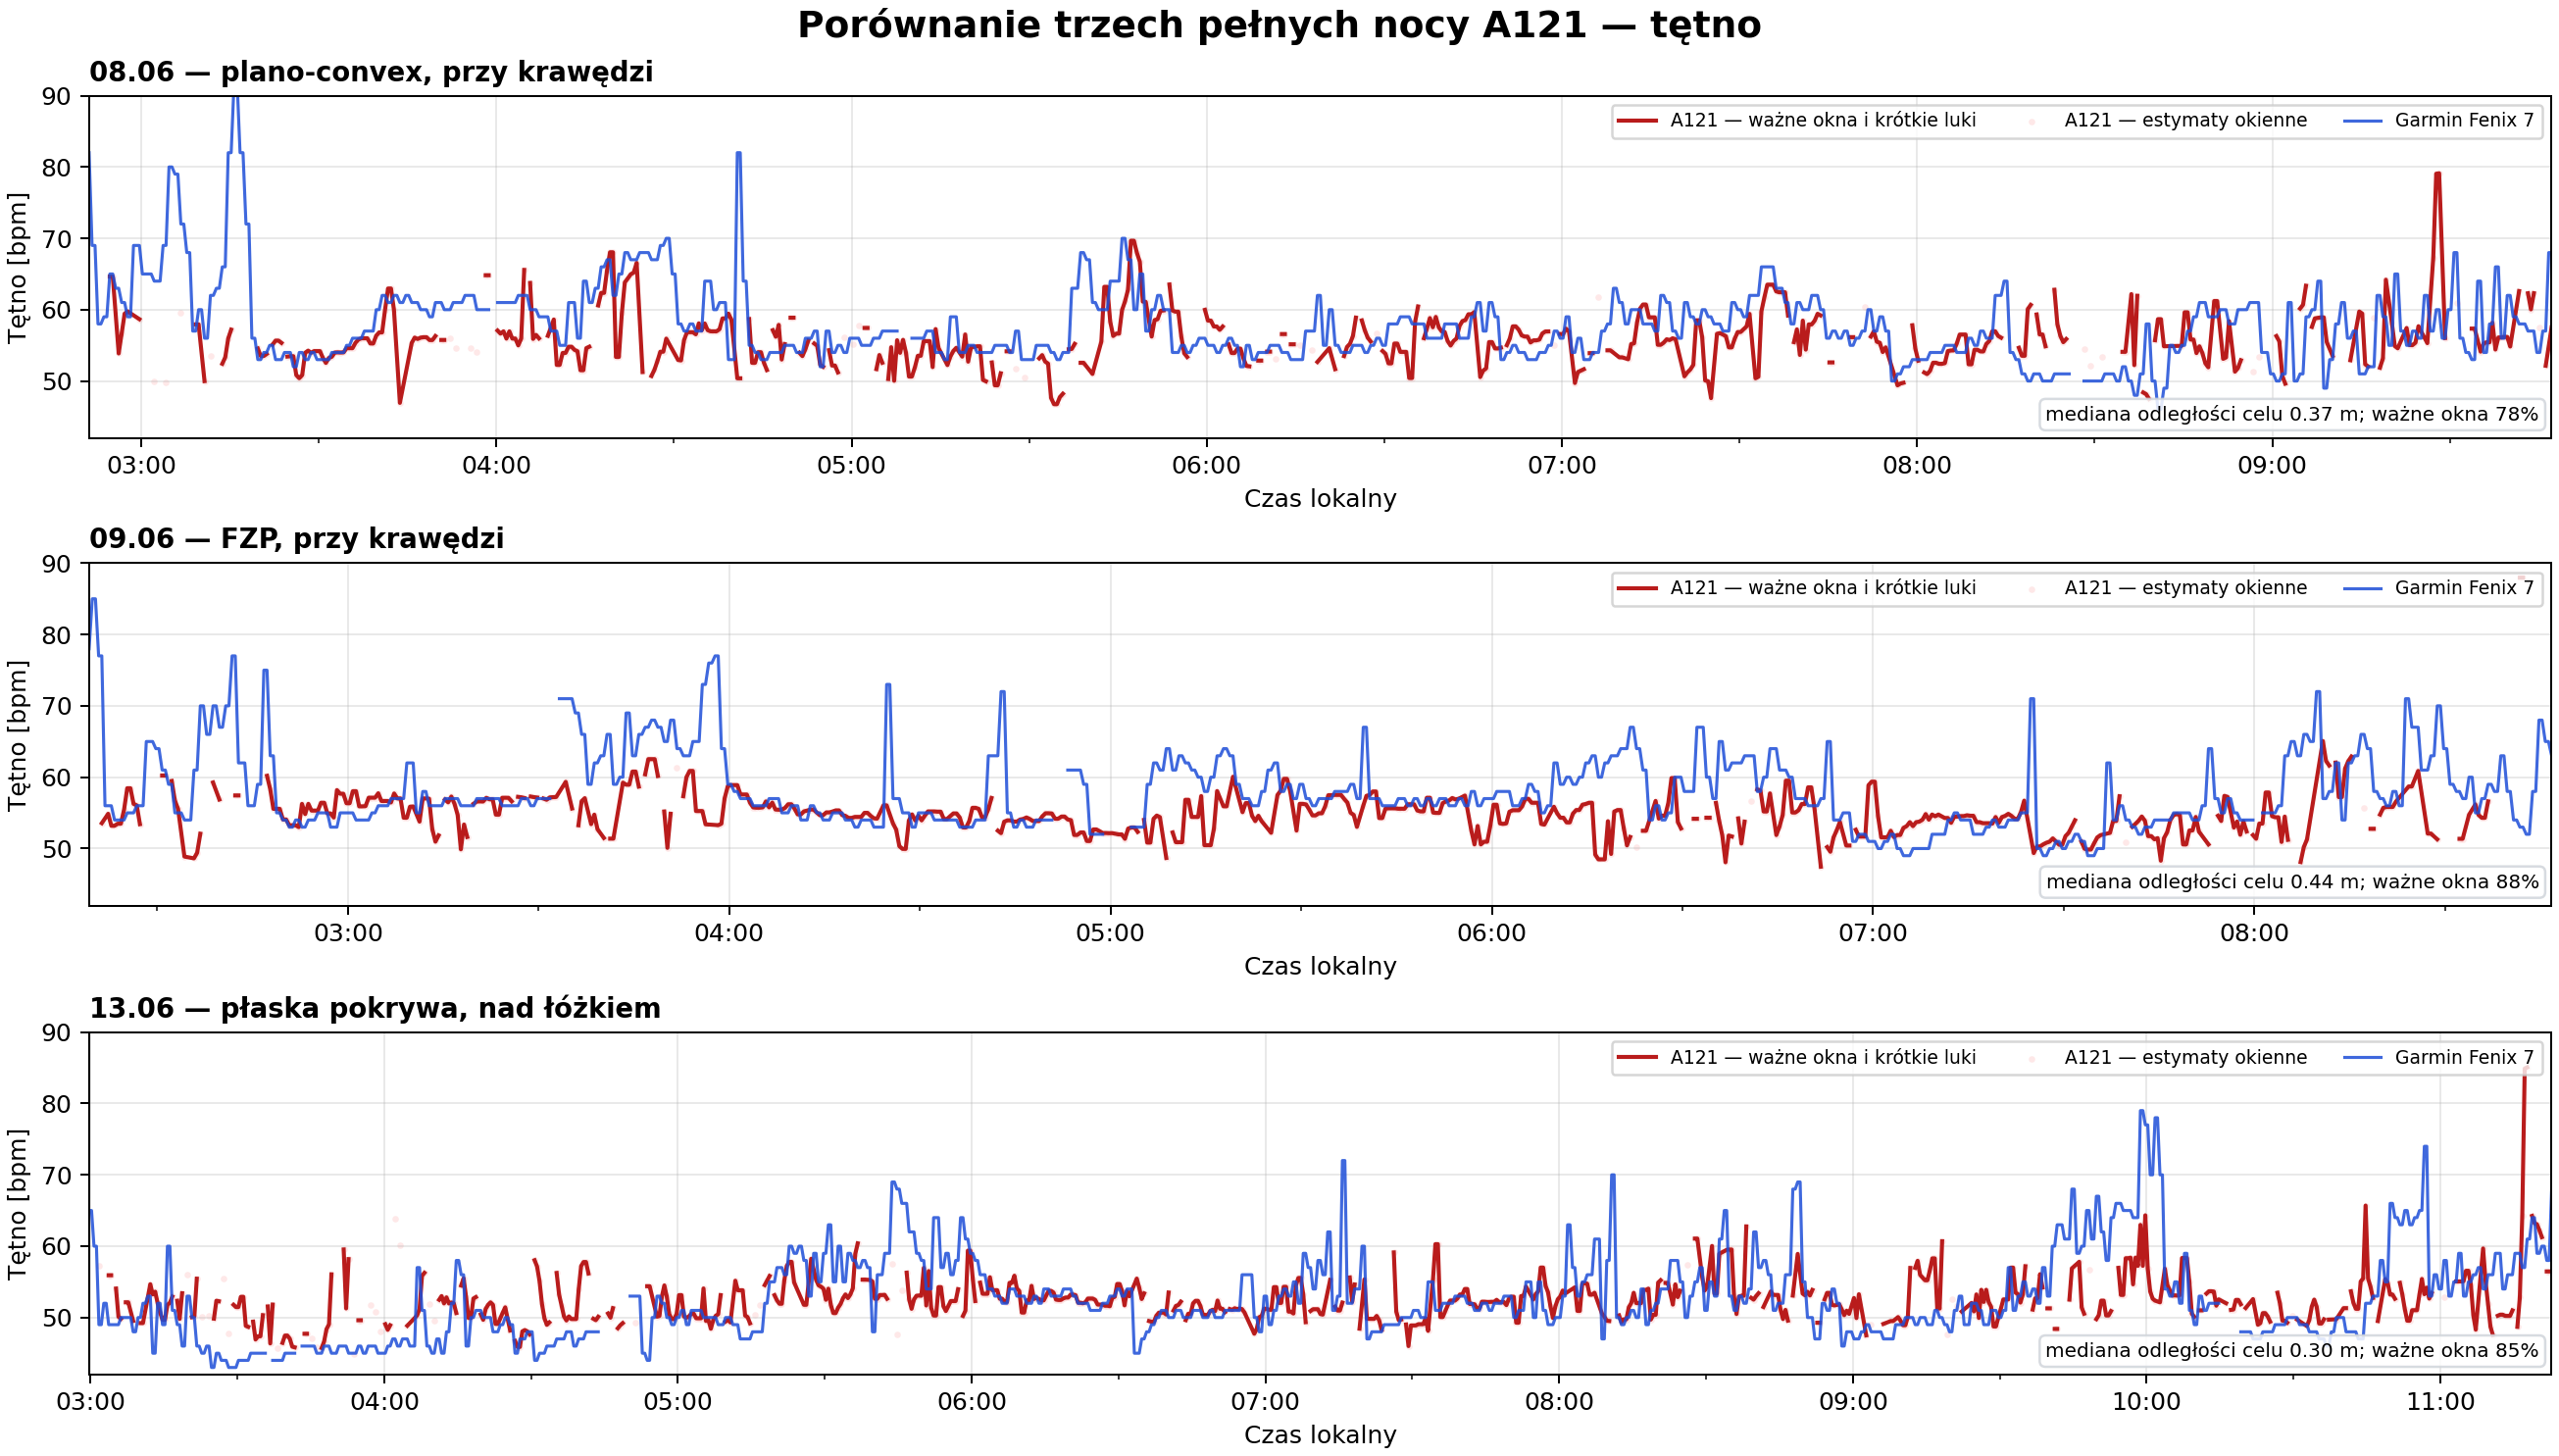
\includegraphics[width=\textwidth]{sen_porownanie_konfiguracji_tetno.png}
    \caption[Tętno w trzech pełnych nocach]{Tętno A121 i~Garmin Fenix~7 dla
    trzech pełnych nocy głównego porównania. Linia A121 łączy wyłącznie ważne
    okna i~krótkie przerwy ruchowe; długich luk nie interpolowano.}
    \label{fig:sen-porownanie-hr}
\end{figure}

\begin{figure}[p]
    \centering
    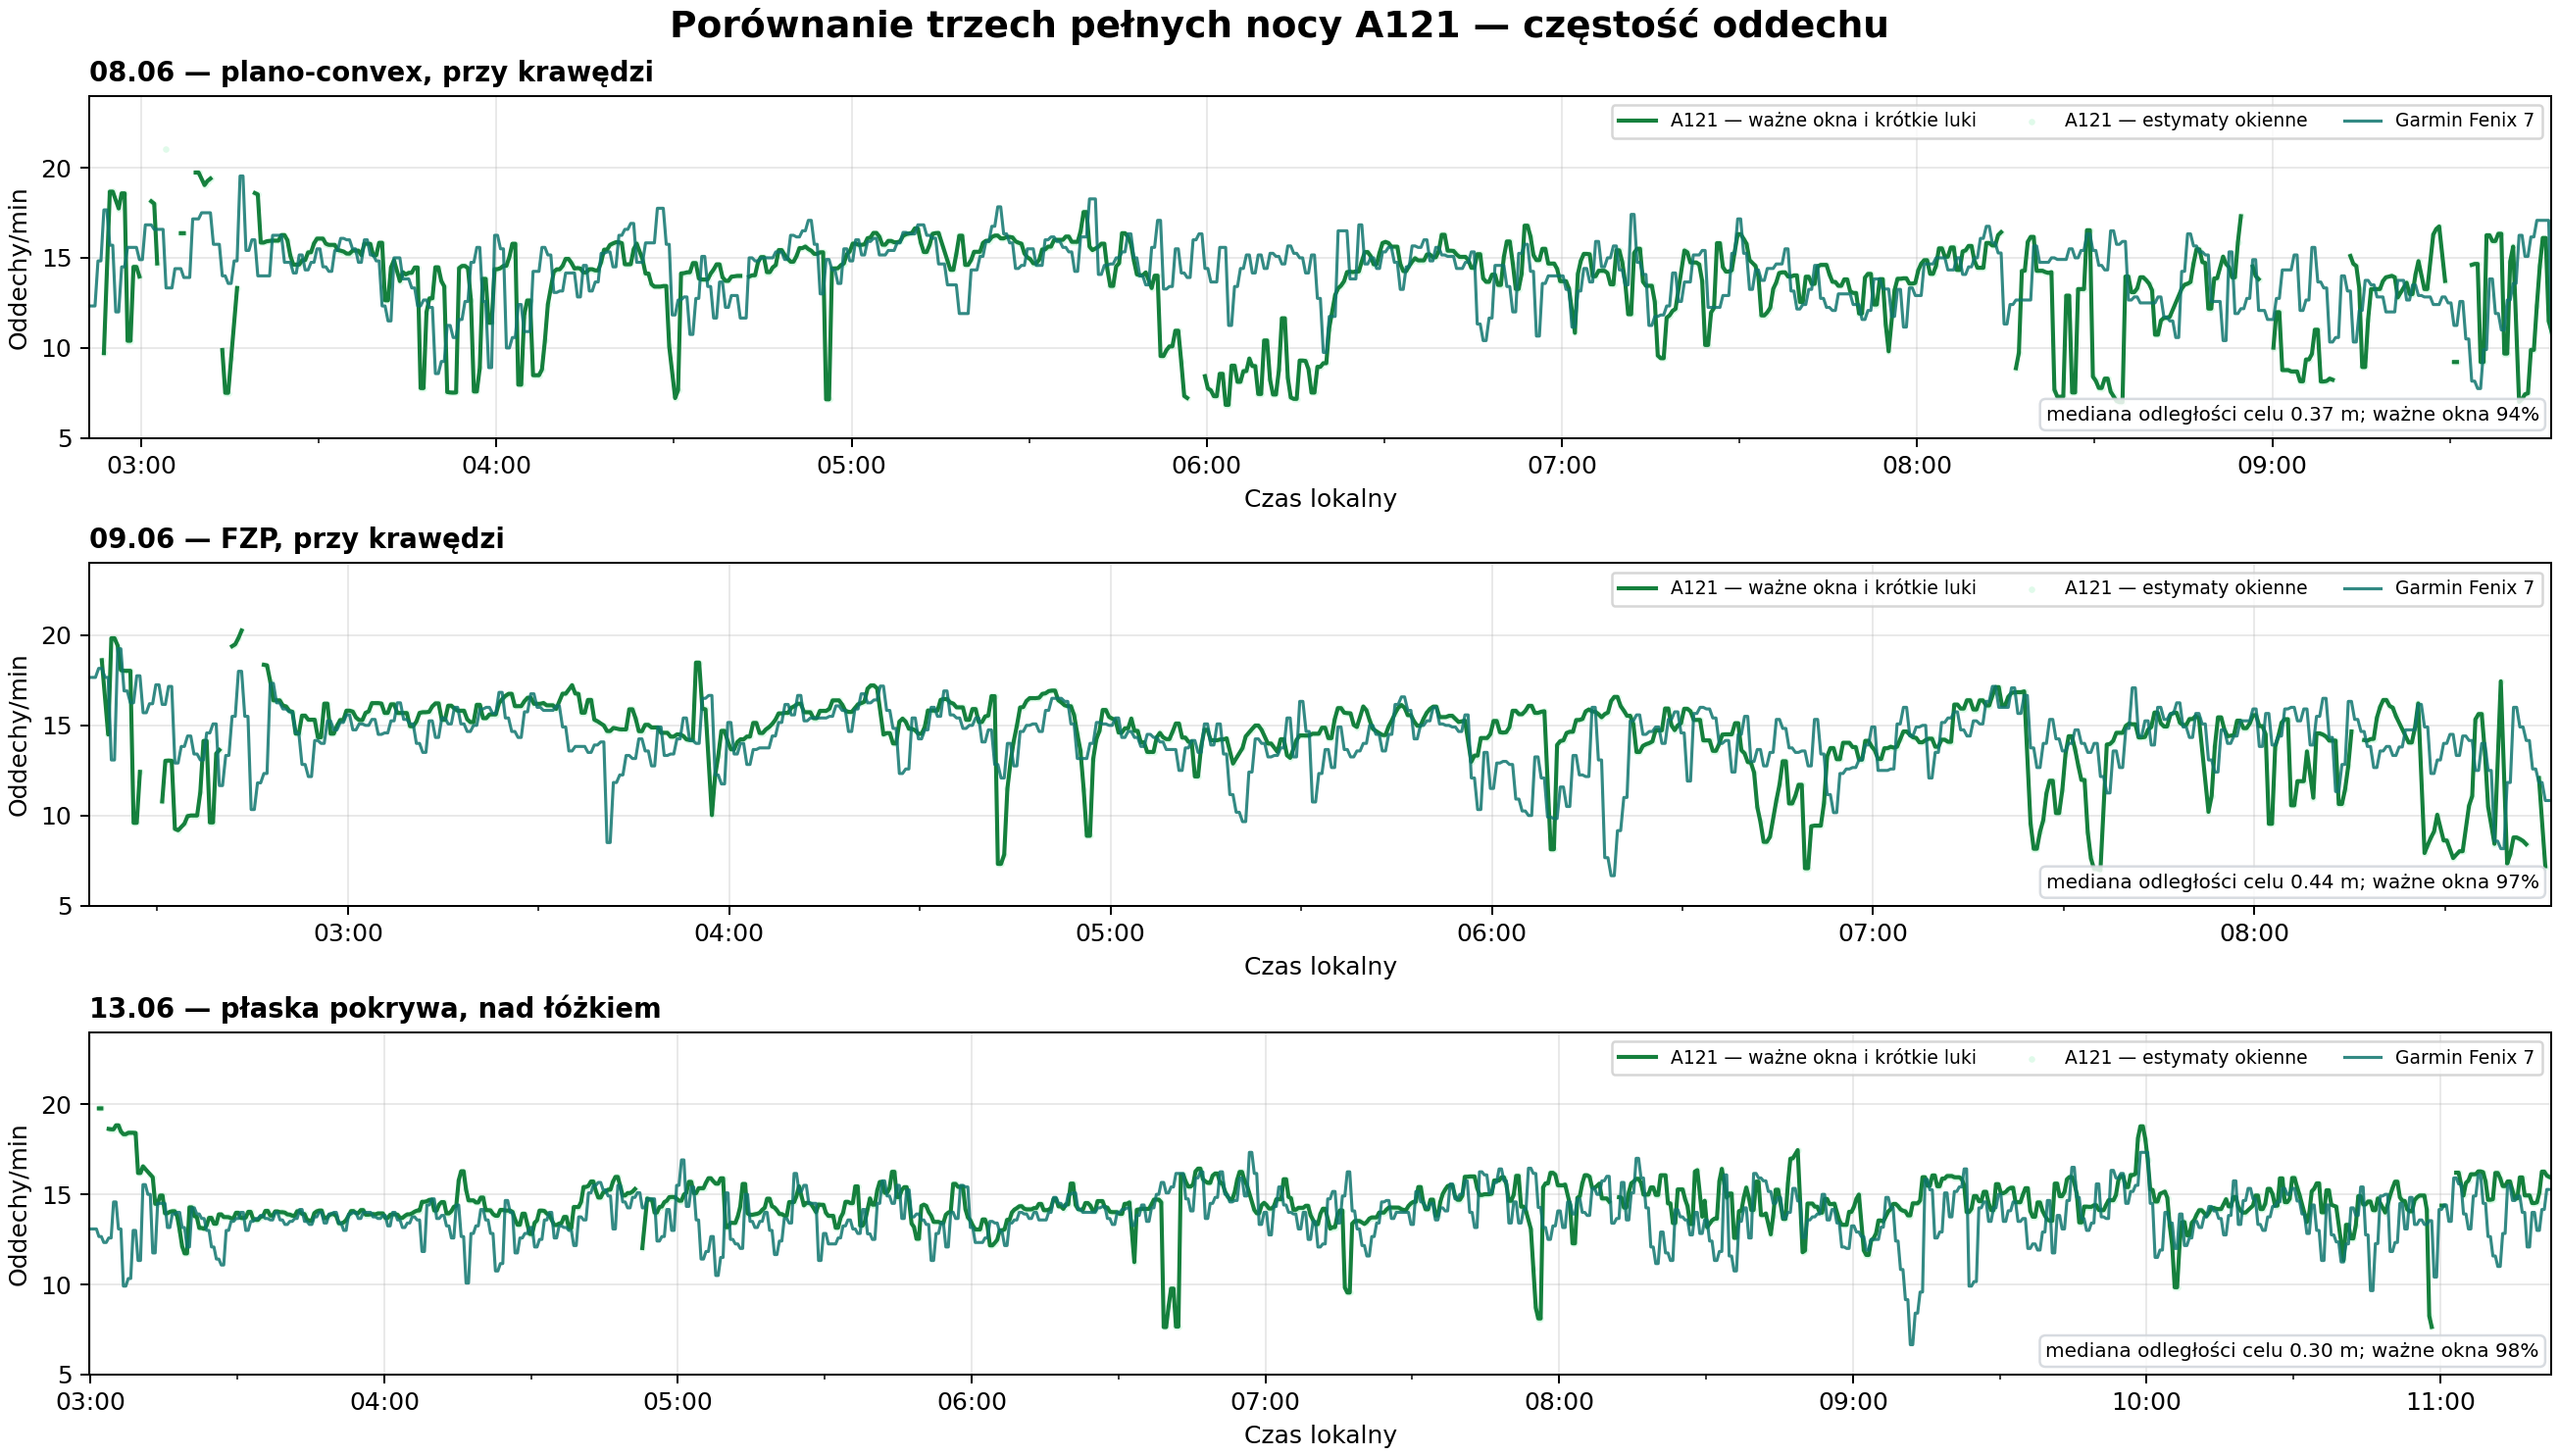
\includegraphics[width=\textwidth]{sen_porownanie_konfiguracji_oddech.png}
    \caption[Częstość oddechu w trzech pełnych nocach]{Częstość oddechu A121
    i~Garmin Fenix~7. Ustawienie z~płaską pokrywą nad łóżkiem daje najbardziej
    ciągły przebieg, ale widoczne krótkie odchylenia nadal należy interpretować
    razem z~odrzucaniem okien po ruchu.}
    \label{fig:sen-porownanie-rr}
\end{figure}

\begin{figure}[p]
    \centering
    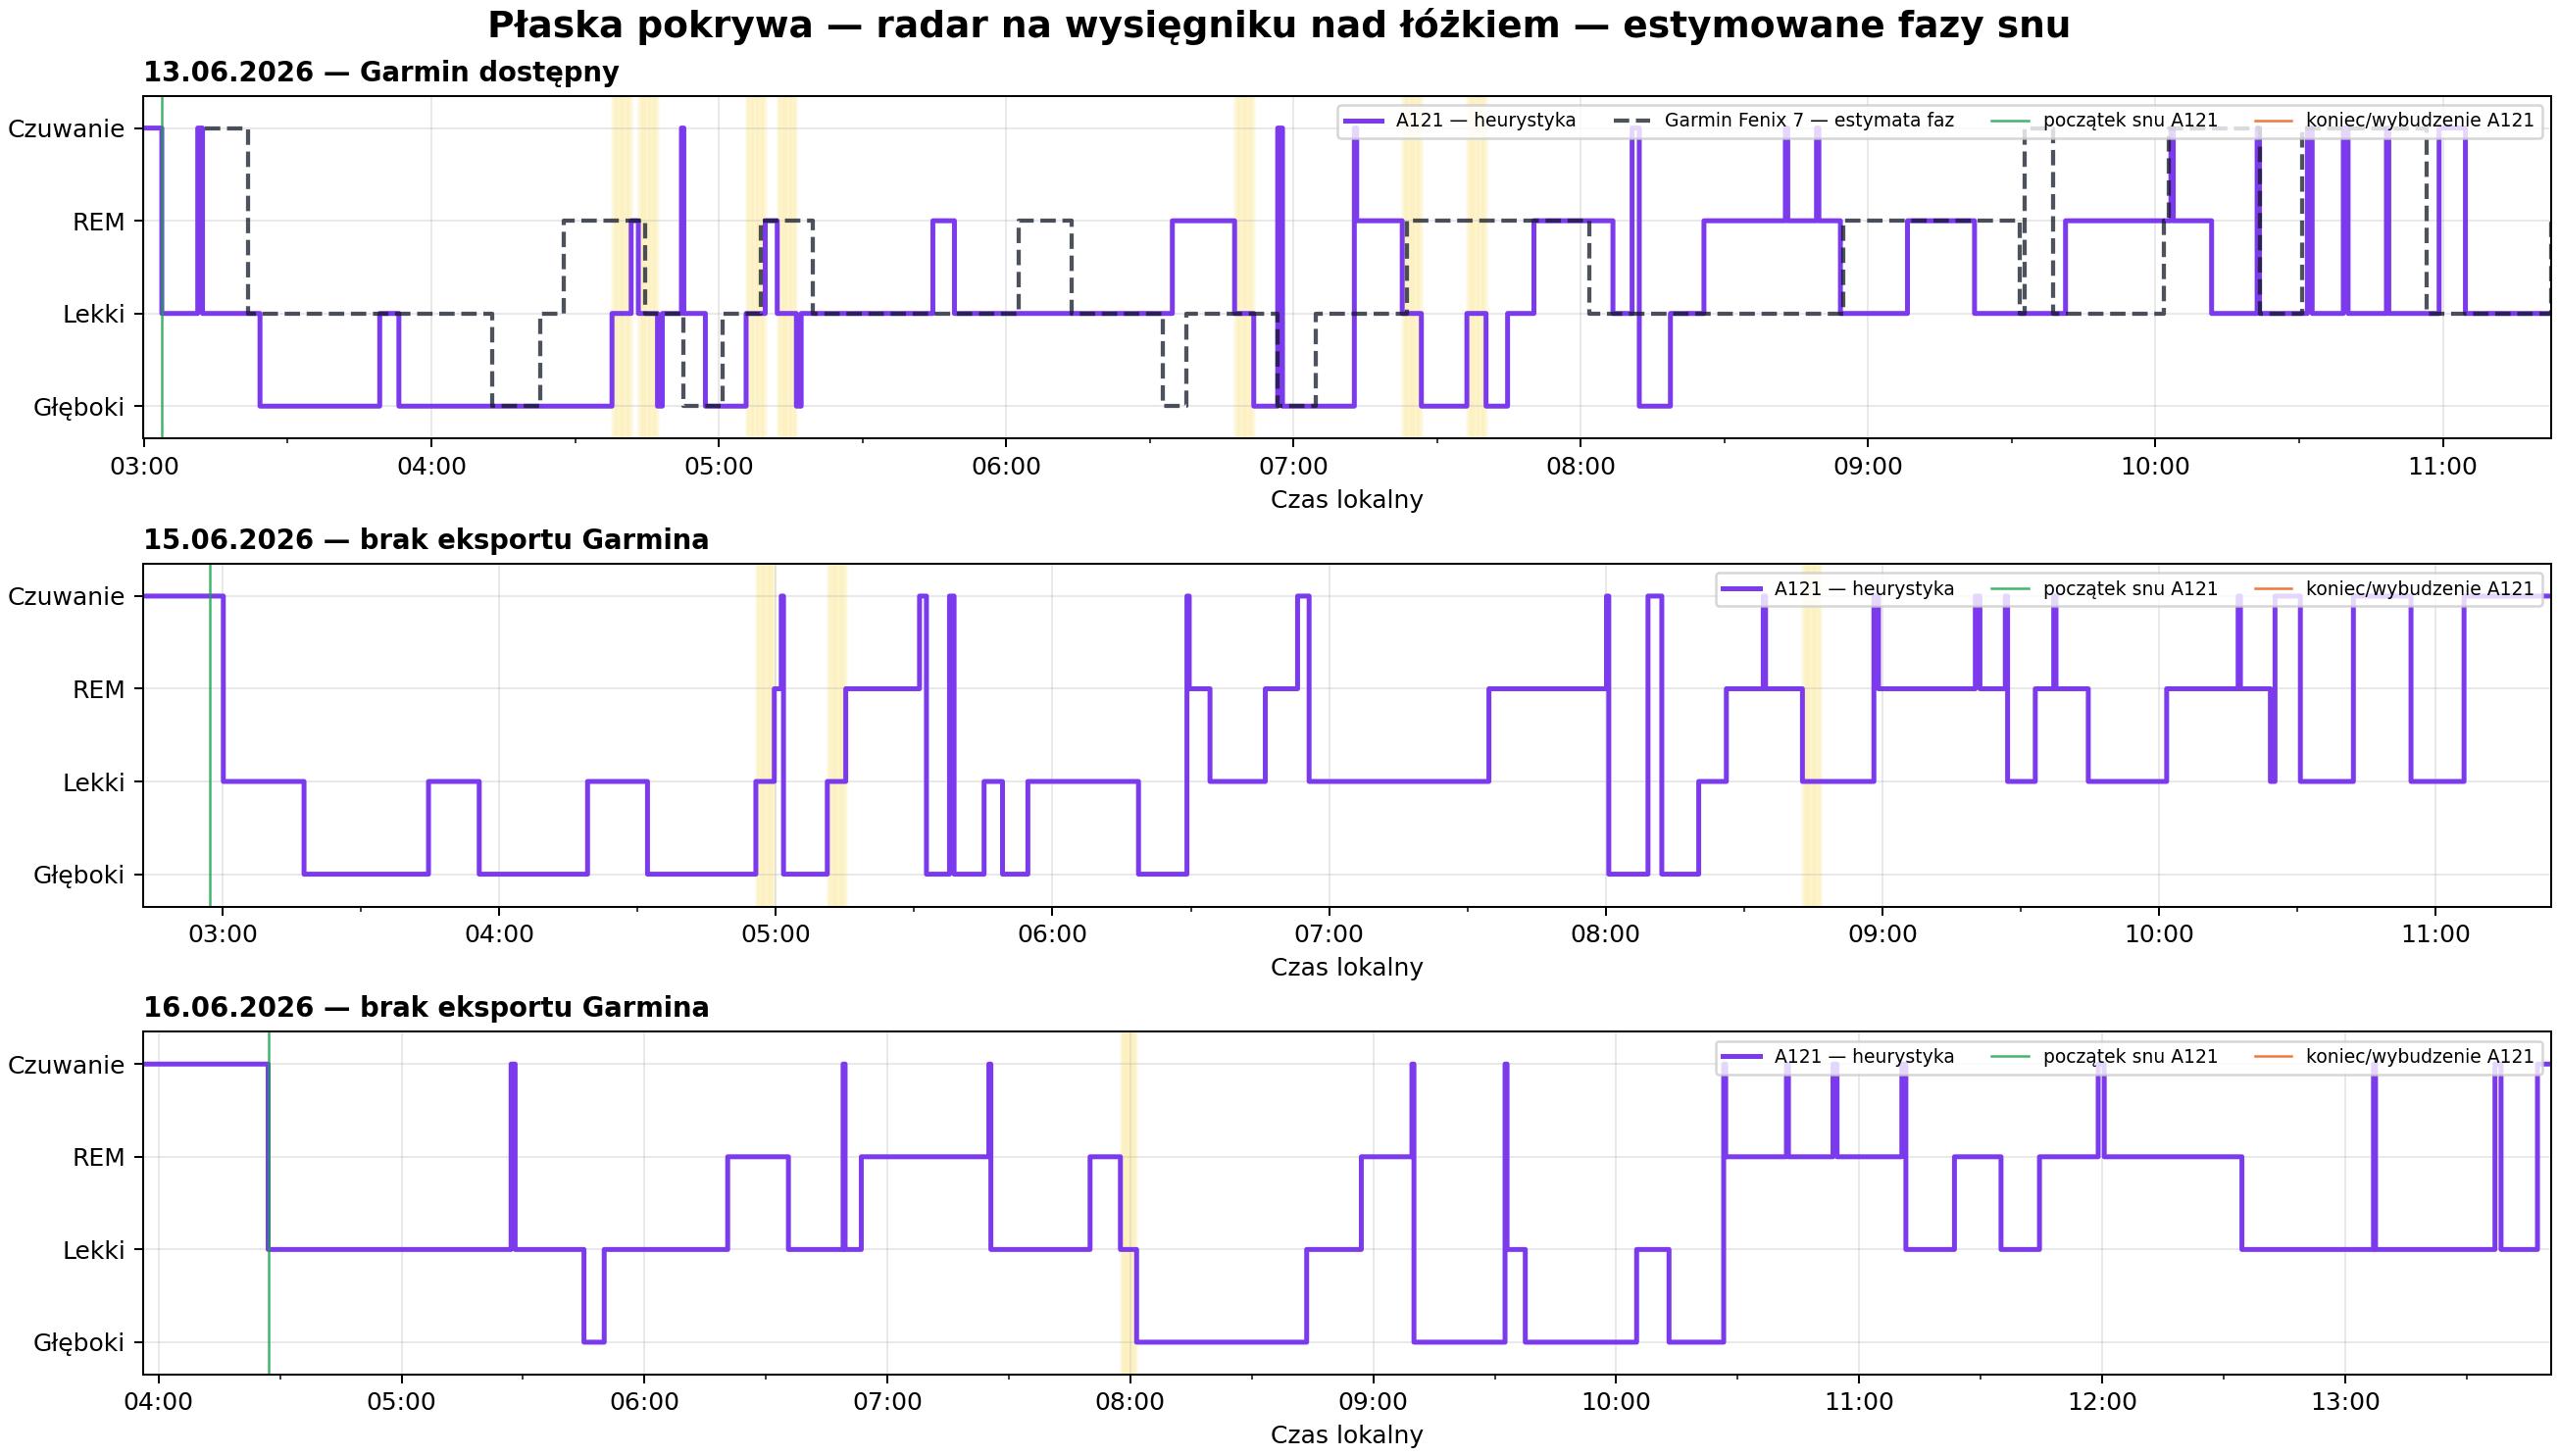
\includegraphics[width=\textwidth]{sen_flat_nad_lozkiem_fazy.png}
    \caption[Fazy snu z płaską pokrywą nad łóżkiem]{Trzy pełne noce z~płaską
    pokrywą i~radarem na wysięgniku nad łóżkiem. Dla nocy~3 dostępna jest
    estymata faz Garmina; dwa pozostałe panele są radarowe i~nie powinny być
    interpretowane jako zweryfikowane stadia snu.}
    \label{fig:sen-flat-fazy}
\end{figure}

\begin{figure}[p]
    \centering
    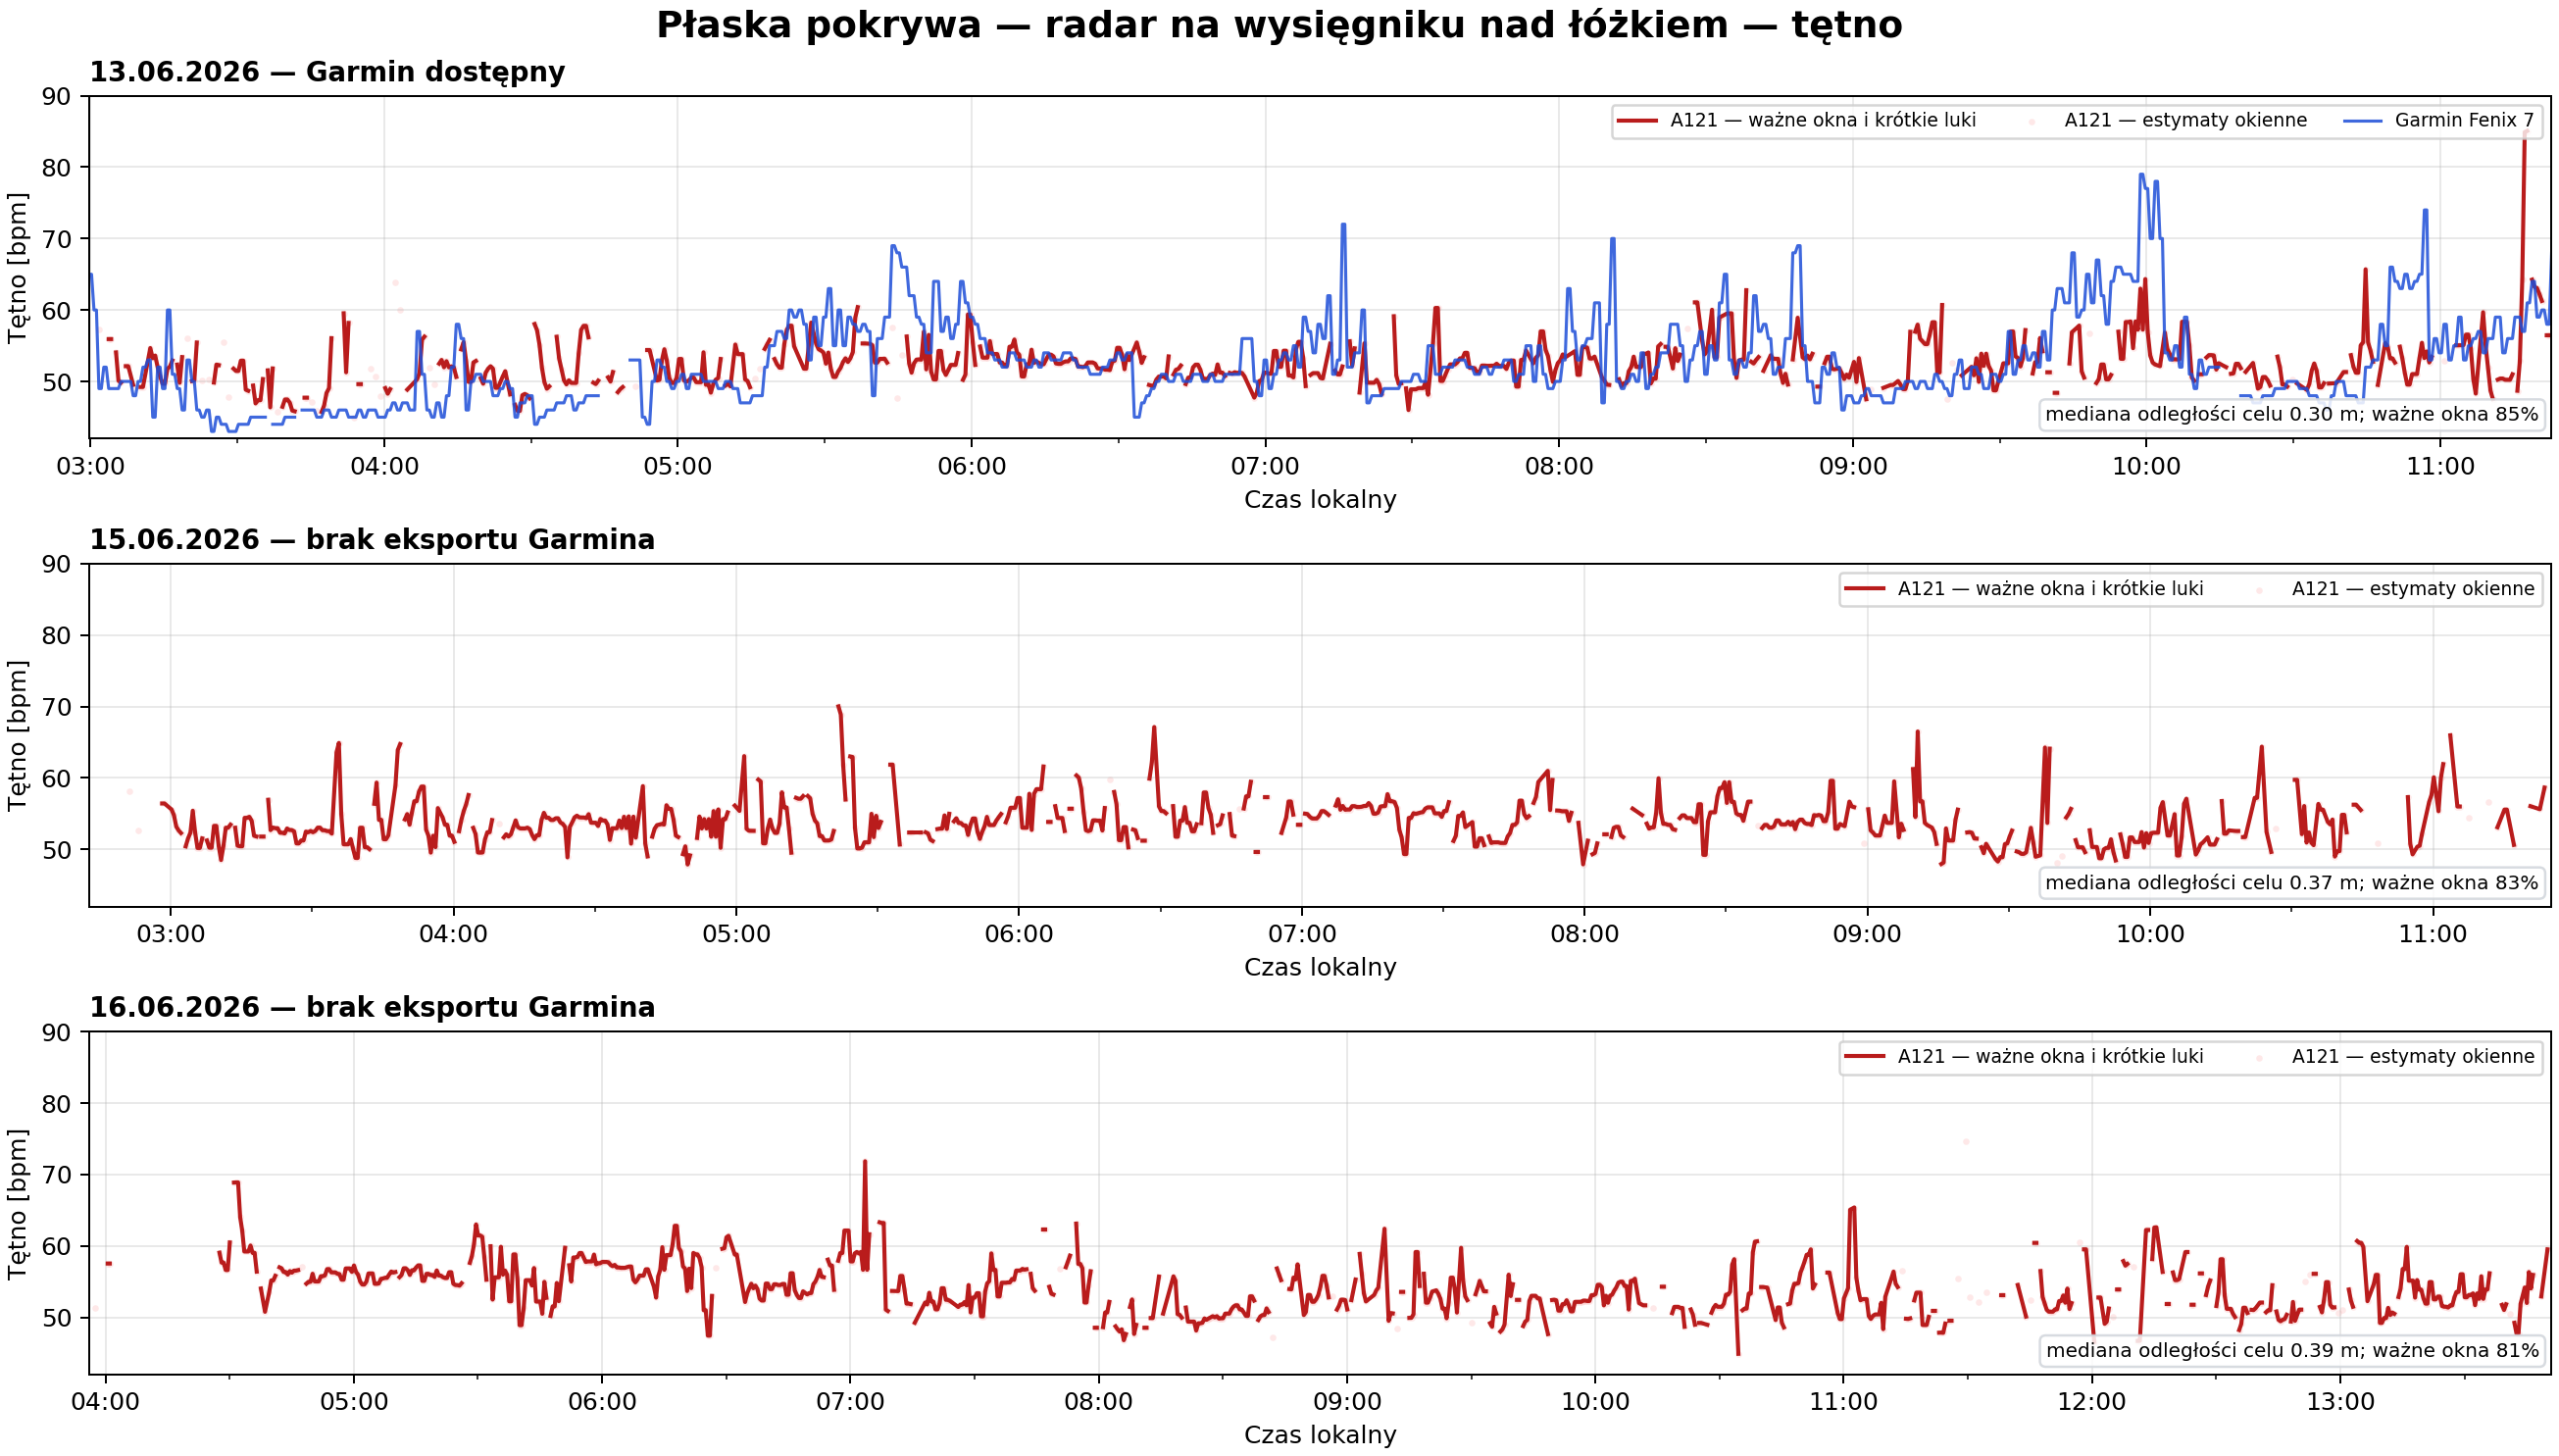
\includegraphics[width=\textwidth]{sen_flat_nad_lozkiem_tetno.png}
    \caption[Tętno z płaską pokrywą nad łóżkiem]{Tętno w~trzech pełnych
    nocach z~ustawieniem nad łóżkiem. Mediana śledzonej odległości celu
    wynosiła \SIrange{0.30}{0.39}{m}, a~ważny wynik HR był dostępny w~około
    81--85\% okien. Dla nocy~3 trend A121 można bezpośrednio zestawić
    z~Garminem; długich luk nie interpolowano.}
    \label{fig:sen-flat-hr}
\end{figure}

\begin{figure}[p]
    \centering
    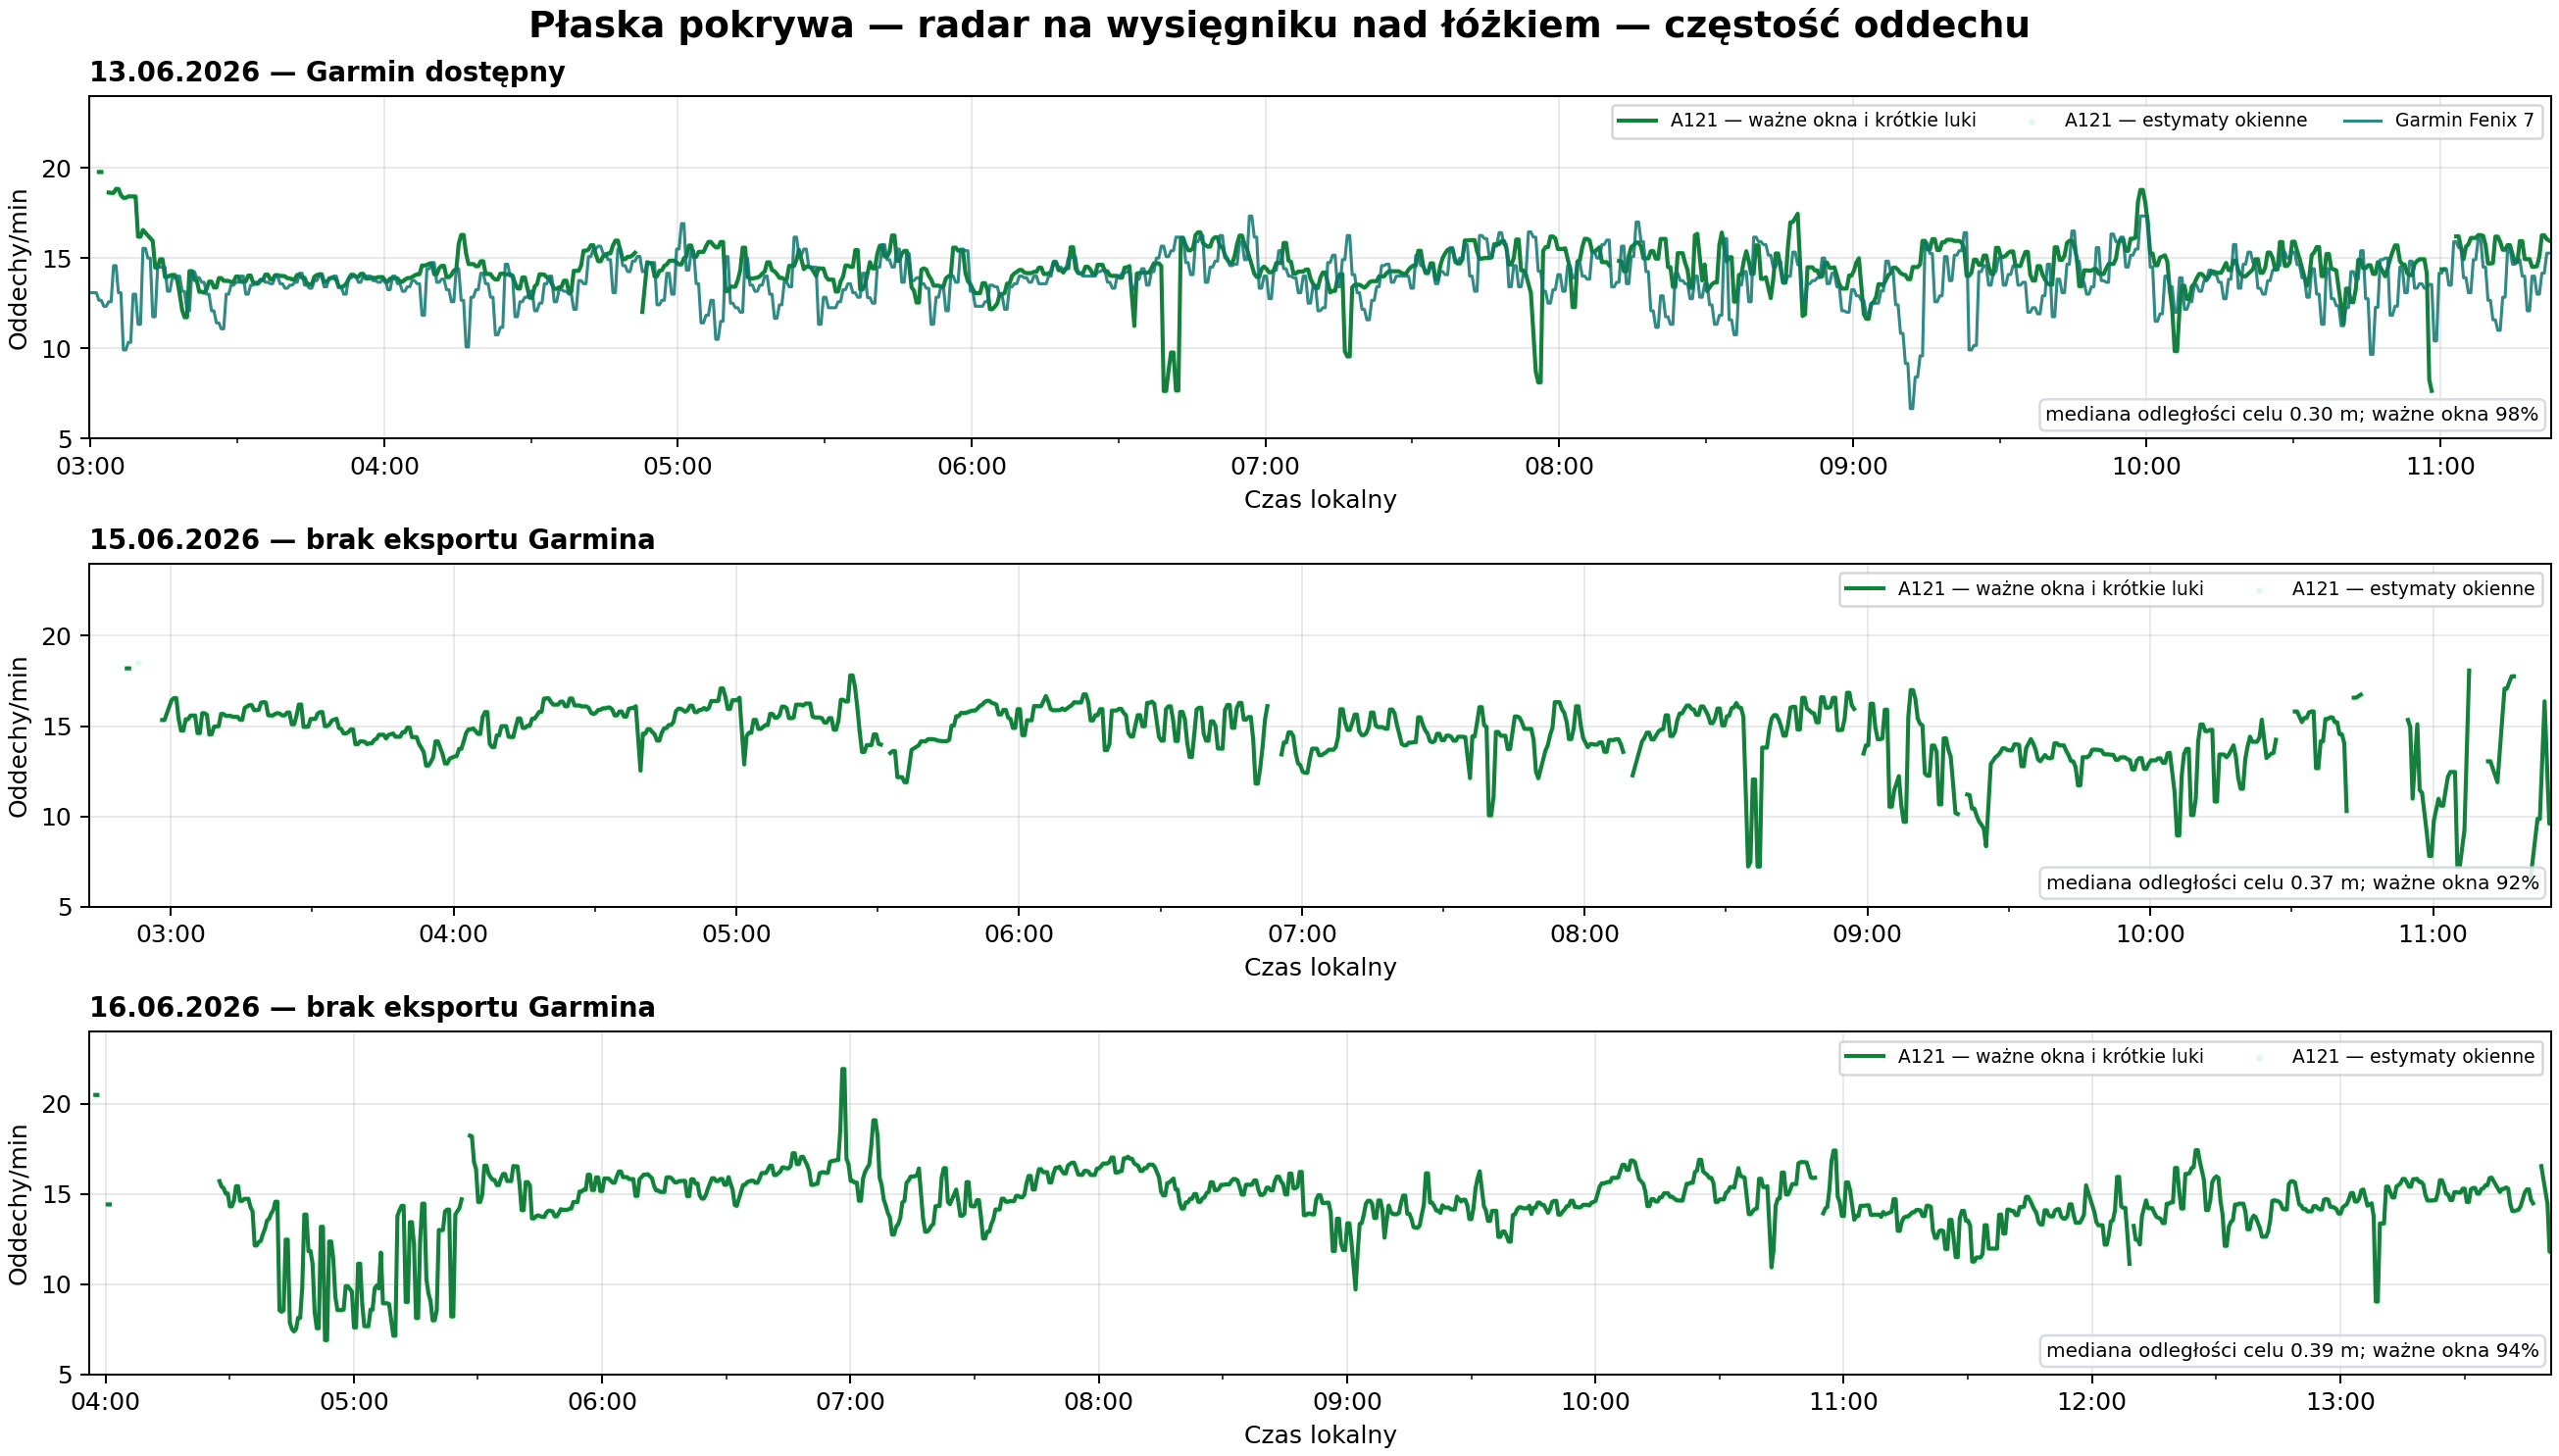
\includegraphics[width=\textwidth]{sen_flat_nad_lozkiem_oddech.png}
    \caption[Częstość oddechu z płaską pokrywą nad łóżkiem]{Częstość oddechu
    w~trzech pełnych nocach z~płaską pokrywą. Estymata była dostępna w~około
    92--98\% okien i~przez większość czasu pozostawała w~spójnym zakresie;
    tylko dla nocy~3 zachował się równoległy eksport Garmina.}
    \label{fig:sen-flat-rr}
\end{figure}

\section{Ograniczenie interpretacyjne: amplituda dominującego odbicia}

\begin{table}[H]
\centering
\caption{Amplituda dominującego odbicia a~zgodność z~celem.}
\label{tab:amplitudy}
\small
\resizebox{\textwidth}{!}{%
\begin{tabular}{@{}lrrrr@{}}
\toprule
Nagranie & Mediana ampl. & Mediana odl. & Mediana odl. & Udział okien \\
 & piku [j.u.] & celu [m] & piku [m] & $|\Delta d|\leq$\SI{0.10}{m} \\
\midrule
Noc 1, plano-convex przy krawędzi & 1665  & 0,37 & 0,15 & 0,316 \\
Noc 2, FZP przy krawędzi          & 17516 & 0,44 & 0,12 & 0,012 \\
Noc 3, płaska nad łóżkiem         & 23133 & 0,30 & 0,10 & 0,224 \\
Przypadek negatywny, hiperboliczna & 811   & 1,62 & 1,98 & 0,094 \\
\bottomrule
\end{tabular}%
}
\end{table}

Tabela~\ref{tab:amplitudy} pokazuje, dlaczego nie należy utożsamiać wysokości
dominującego piku z~jakością sygnału z~klatki. Dla FZP jedynie
\textbf{1,2\%} porównywalnych okien miało pik w~promieniu \SI{10}{cm} od
śledzonego celu. Nawet w~dobrej nocy z~płaską pokrywą mediana piku leżała przy
\SI{0.10}{m}, a~celu przy \SI{0.30}{m}. Wysokie amplitudy mogły więc pochodzić
od krawędzi łóżka, pościeli albo obudowy, a~nie bezpośrednio od klatki.

Z~tego powodu w~niniejszej pracy przyjęto następującą hierarchię wyników:
\begin{enumerate}
  \item zgodność HR/RR z~Garminem --- wynik \textbf{podstawowy},
  \item zgodność faz snu --- wynik \textbf{drugorzędny},
  \item surowa amplituda piku --- wyłącznie \textbf{kontekst inżynierski}.
\end{enumerate}

\paragraph{Negatywny przypadek geometrii.} Osobny zapis z~soczewką
hiperboliczną i~medianą celu \SI{1.62}{m} potraktowano jako ilustrację
wrażliwości na ustawienie. Przy odchyleniu osi o~ponad \SI{60}{\degree} od
normalnej dostępność surowego HR spadła do 51,4\%, a~MAE względem Garmina
wzrósł do \SI{6.4}{bpm}; dla oddechu MAE wyniósł około
3,0~oddechy/min. Wynik jest wyraźnie gorszy od trzech konfiguracji
z~tabeli~\ref{tab:sen-jakosc}. Nie jest to kontrolowany dowód przeciw soczewce
hiperbolicznej, lecz praktyczny przykład, że duży dystans połączony ze złym
kątem może zniweczyć korzyść z~węższej wiązki.

\section{Dyskusja wyników nocnych}
Częstość oddechu była zgodna z~wynikiem Garmina lepiej niż tętno. Jest to
spójne z~większą amplitudą ruchu oddechowego i~mniejszymi wymaganiami na SNR;
składowa sercowa jest słabsza i~łatwiej ulega zakłóceniu przez ruch całego
ciała, harmoniczne oddechu oraz zmianę dominującego reflektora.

W~pomiarze nocnym początkowe skierowanie radaru na klatkę nie gwarantuje
utrzymania tej geometrii przez wiele godzin. Badany zmienia pozycję, a~klatka
przesuwa się poprzecznie i~obraca względem osi czujnika. Wąska wiązka soczewki
skupiającej może wtedy dać wysoką amplitudę odbicia od niewłaściwego obiektu,
podczas gdy szersze pole widzenia płaskiej pokrywy nadal obejmuje część
tułowia. Taki mechanizm jest zgodny zarówno z~najmniejszym średnim obciążeniem
tętna w~nocy~3, jak i~z~ciągłymi przebiegami trzech nocy nad łóżkiem.
Nie należy jednak przypisywać całej poprawy samej pokrywie: jednocześnie zmieniono
położenie radaru z~boku łóżka na wysięgnik nad tułowiem. Wynik pokazuje
przewagę \emph{konkretnej pary} szeroka wiązka--tolerancyjna geometria, a~nie
uniwersalny ranking elementów optycznych.

Najważniejsze ograniczenia badania to jedna osoba, różne ustawienia między
nocami, brak eksportu Garmina dla dwóch z~trzech pełnych nocy nad łóżkiem oraz
brak polisomnografii. Garmin jest konsumenckim źródłem porównania, a~nie
złotym standardem. Z~tego powodu wyników nie należy interpretować jako
rankingu soczewek ani walidacji klinicznej algorytmu snu. Noc z~soczewką
hiperboliczną przy medianie \SI{1.62}{m} pozostaje świadomie wyłączona
z~rankingu soczewek, ponieważ ponad \SI{60}{\degree} odchylenia od normalnej
czyniło geometrię nieporównywalną. Może służyć jedynie jako negatywny przypadek
pokazujący wagę wycelowania.

\todo{Powtórzyć noc z~soczewką hiperboliczną przy większym dystansie,
utrzymując oś możliwie prostopadle do klatki. Udokumentować kąt i~dystans oraz
porównać z~płaską pokrywą na tym samym mocowaniu.}

% ---------------------------------------------------------------------
\chapter{Dalsze zastosowania i eksperymenty}

\todo{Rozdział rezerwowy --- na kolejne eksperymenty, które powstaną
w~trakcie pracy.}

\section{Detekcja bezdechów}
\miejsce{Możliwość wykrywania pauz oddechowych z~sygnału fazowego;
kryteria (pauza $>$\SI{10}{s}), weryfikacja.}

\section{Pomiar na większych dystansach}
Wstępny test na dystansie około \SI{2}{m} wykazał, że soczewka
plano-convex zwiększyła amplitudę tylko o~około 13\%, ale dała znacznie
bardziej wiarygodną estymatę tętna (54,5 wobec 83,2~bpm dla wariantu bez
soczewki). Jest to kolejny argument, że amplituda nie jest wystarczającym
kryterium decyzyjnym. Planowany test granicy zasięgu wykorzystuje jedną
soczewkę hiperboliczną, stałą konfigurację, oddech \SI{0.2}{Hz} narzucony
metronomem oraz odcinki wstrzymania oddechu. Granicę użyteczności należy
zdefiniować przez trafienie zadanej częstości i~SNR, a~nie przez samą
widoczność przebiegu.

\section{Pomiar przez przeszkody}
Wyniki literaturowe z~sekcji~\ref{sec:materialy-radar} wskazują, że cienka,
sucha odzież powinna mieć mniejszy wpływ niż zawilgocona tkanina albo
wielowarstwowa kołdra. Należy jednak raportować konkretny materiał, grubość,
wilgotność i~kąt, ponieważ pojęcie ,,penetracji'' bez tych danych jest
niejednoznaczne. Praktycznym rozwinięciem jest przeplatany pomiar bez
przeszkody i~przez tę samą suchą kołdrę, oddzielnie dla HB100 i~A121.

\section{Wielu badanych i uogólnialność}
\miejsce{Wszystkie dotychczasowe wyniki pochodzą od jednego badanego.
Rozszerzenie na grupę --- kluczowe dla wiarygodności modeli uczonych.}

\section{Zastosowanie sieci neuronowych do klasyfikacji snu}
\miejsce{Zastąpienie heurystycznego klasyfikatora faz snu modelem uczonym na
danych z~Garmina jako etykietach; ograniczenia takiego podejścia (etykiety
referencyjne same są estymatami).}

% =====================================================================
% ZAKOŃCZENIE
% =====================================================================
\chapter{Podsumowanie i wnioski końcowe}

\todo{Zebrać wnioski z~części II i~III, odnieść się do celów postawionych
w~rozdziale~1.}

Najważniejsze ustalenia inżynierskie uzyskane dotychczas:
\begin{itemize}
  \item Zbudowano kompletny tor pomiarowy dla radaru HB100 --- od analogowego
  wzmacniacza i~filtru ($\approx121\times$) po estymację parametrów witalnych
  --- oraz zintegrowano radar Acconeer~A121 pracujący na surowych danych
  Sparse~IQ.
  \item W~równoczesnych nagraniach HB100 wykrywał sterowany, pogłębiony oddech
  i~jego zatrzymanie do \SI{100}{cm}; podczas wstrzymania RMS malał o~
  \SIrange{18.4}{24.6}{dB}. Jednokanałowy sygnał był jednak zdominowany przez
  harmoniczne w~10 z~12 bloków i~nie zachowywał stabilnie kierunku
  wdech--wydech. Opracowany estymator konsensusu harmonicznych odzyskał
  w~12 blokach powtarzanej serii \SIrange{30}{100}{cm} rytm
  \SIrange{0.198}{0.204}{Hz} przy zadanych \SI{0.20}{Hz}. Jest to jednak
  jedynie warunkowa estymacja rytmu dla dużych, pełnych oddechów po kontroli
  jakości, a~nie rekonstrukcja przemieszczenia ani faz cyklu. W~pojedynczym
  reteście \SI{150}{cm} wartości \SI{0.190}{Hz} i~\SI{0.202}{Hz} miały
  marżę jakości zaledwie 2,9 i~2,1 przy progu 2,0, dlatego są tylko
  granicznym wskazaniem rytmu; estymacja faz wdech--wydech nie była tam
  użyteczna. A121 osiągał w~powtarzanej serii 95,9--99,3\% opisowej zgodności
  kierunku, a~w~reteście \SI{150}{cm} 96,7\%, dlatego jego faza I/Q pozostaje
  właściwym wejściem do analizy faz cyklu. HB100 może pełnić co najwyżej rolę
  pomocniczego wskaźnika rytmu, wyraźnie słabszego informacyjnie od A121.
  \item Na dystansie \SIrange{0.5}{1.0}{m} system nie jest ograniczony
  amplitudą sygnału: SNR oddechowy wynosi 44--47~dB niezależnie od soczewki
  i~obecności folii aluminiowej. Zysk anteny przekłada się na stabilność
  śledzenia celu, a~nie na wykrywalność oddechu.
  \item Retest na dystansie \SI{2}{m} potwierdził, że folia aluminiowa nie
  daje powtarzalnego wzmocnienia. Zmiana geometrii z~naturalnej na prawie
  prostopadłą zwiększyła natomiast echo o~około \SI{11}{dB}; właściwe
  wycelowanie radaru miało więc znacznie większe znaczenie niż metalowa łata.
  \item W~trzech pełnych nocach średnie obciążenie częstości oddechu względem
  Garmin~Fenix~7 nie przekroczyło $0{,}7$~oddechu/min, choć okienny MAE
  wynosił 1,3--2,0~oddechu/min; dla tętna MAE wynosił 3,8--3,9~bpm.
  Rozbieżności w~fazach snu wskazują na ograniczenia heurystycznego
  klasyfikatora i~motywują jego dalszą walidację lub zastąpienie modelem
  uczonym.
\end{itemize}

\section{Kierunki dalszych prac}
\miejsce{Sieci neuronowe do klasyfikacji faz oddechu
(rozdział~\ref{chap:sieci}), rozszerzenie badania na wielu uczestników,
walidacja względem polisomnografii.}

% =====================================================================
\begin{thebibliography}{99}
\bibitem{acconeer_lens}
Acconeer AB, \emph{Lens design --- Acconeer docs}, dokumentacja techniczna
A121, \url{https://docs.acconeer.com/en/latest/integration/lens_design.html}
(dostęp: 15.07.2026).

\bibitem{acconeer_handbook}
Acconeer AB, \emph{A121 documentation and software},
\url{https://developer.acconeer.com/home/a121-docs-software/}
(dostęp: 15.07.2026).

\bibitem{acconeer_datasheet}
Acconeer AB, \emph{A121 Pulsed Coherent Radar Sensor Data Sheet}, wersja 1.8,
\url{https://developer.acconeer.com/download/a121-datasheet/}
(dostęp: 15.07.2026).

\bibitem{acconeer_sparse_iq}
Acconeer AB, \emph{Interpreting radar data --- Sparse IQ},
\url{https://docs.acconeer.com/en/latest/radar_data_and_control/a121/interpreting_radar_data.html}
(dostęp: 15.07.2026).

\bibitem{waveshare_a121}
Waveshare, \emph{A121 Range Sensor --- documentation},
\url{https://www.waveshare.com/wiki/A121_Range_Sensor}
(dostęp: 15.07.2026).

\bibitem{mileseey_d2}
MILESEEY, \emph{D2 Laser Distance Meter --- specifications},
\url{https://mileseeyrussia.ru/dalnomer-mileseey-d2/}
(dostęp: 15.07.2026).

\bibitem{infineon_fmcw}
Infineon Technologies, \emph{FMCW Radar Digital Signal Processing}, materiał
szkoleniowy,
\url{https://www.infineon.com/dgdl/Infineon-FMCW_RADAR_Digital_Signal_Processing_Handout-Training-v01_00-EN.pdf?fileId=8ac78c8c8929aa4d018a178075b06be9}
(dostęp: 15.07.2026).

\bibitem{wallace2018}
J.~W. Wallace, R. Mehmood, M.~A. Jensen, \emph{4--40 GHz Transmission
Measurement of Indoor Building Materials at Normal Incidence}, 2018 IEEE
International Symposium on Antennas and Propagation and USNC/URSI National
Radio Science Meeting, 2018,
\url{https://doi.org/10.1109/APUSNCURSINRSM.2018.8609395}.

\bibitem{jun2020}
S.~Y. Jun, D. Caudill, J. Chuang, P.~B. Papazian, A. Bodi, C. Gentile,
J. Senic, N.~T. Golmie, \emph{Penetration Loss at 60 GHz for
Indoor-to-Indoor and Outdoor-to-Indoor Mobile Scenarios}, 14th European
Conference on Antennas and Propagation (EuCAP), 2020,
\url{https://doi.org/10.23919/EuCAP48036.2020.9135581}.

\bibitem{albrecht2023}
N.~C. Albrecht, J.~P. Weiland, D. Langer, M. Wenzel, A. Koelpin,
\emph{Characterization of the Influence of Clothing and Other Materials on
Human Vital Sign Sensing using mmWave Radar}, 53rd European Microwave
Conference (EuMC), 2023,
\url{https://doi.org/10.23919/EuMC58039.2023.10290459}.

\bibitem{landreani2017}
F. Landreani, A. Martin, C. Casellato, E. Pavan, C. Frigo,
P.-F. Migeotte, A. Faini, G. Parati, E. Caiani, \emph{Respiratory Frequency
Estimation from Accelerometric Signals Acquired by Mobile Phone in a
Controlled Breathing Protocol}, Computing in Cardiology, 2017,
\url{https://doi.org/10.22489/CinC.2017.137-402}.

\bibitem{nayak2024}
A. Nayak, M. Bolic, \emph{Smartphone System for Heart Rate and Breathing Rate
Estimation}, IEEE Open Journal of Instrumentation and Measurement, 2024,
\url{https://doi.org/10.1109/OJIM.2024.3477572}.

\bibitem{lsm6ds3}
STMicroelectronics, \emph{LSM6DS3: iNEMO inertial module --- data sheet},
\url{https://www.st.com/resource/en/datasheet/lsm6ds3.pdf}
(dostęp: 15.07.2026).

\bibitem{apple_coremotion}
Apple Inc., \emph{CMMotionManager --- Core Motion documentation},
\url{https://developer.apple.com/documentation/coremotion/cmmotionmanager}
(dostęp: 15.07.2026).

\bibitem{apple_coremotion_interval}
Apple Inc., \emph{deviceMotionUpdateInterval --- Core Motion documentation},
\url{https://developer.apple.com/documentation/coremotion/cmmotionmanager/devicemotionupdateinterval}
(dostęp: 15.07.2026).

\bibitem{garmin_sleep}
\todo{Publikacja o~dokładności szacowania faz snu przez zegarki Garmin
względem polisomnografii.}

\bibitem{hb100_doc}
Agilsense / ST Electronics, \emph{HB100 Microwave Sensor Module Data Sheet},
\url{https://www.theremino.com/wp-content/uploads/files/HB100_Microwave_Sensor_Module_Datasheet.pdf}
(dostęp: 15.07.2026).

\bibitem{mcp6002}
Microchip Technology, \emph{MCP6001/2/4 Operational Amplifier Data Sheet}.
\url{https://ww1.microchip.com/downloads/aemDocuments/documents/MSLD/ProductDocuments/DataSheets/MCP6001-1R-1U-2-4-1-MHz-Low-Power-Op-Amp-DS20001733.pdf}
(dostęp: 15.07.2026).

\bibitem{droitcour2004}
A.~D. Droitcour, O. Boric-Lubecke, V.~M. Lubecke, J. Lin, G.~T.~A. Kovacs,
\emph{Range Correlation and I/Q Performance Benefits in Single-Chip Silicon
Doppler Radars for Noncontact Cardiopulmonary Monitoring}, IEEE Transactions
on Microwave Theory and Techniques, tom~52, s.~838--848, 2004,
\url{https://doi.org/10.1109/TMTT.2004.823552}.

\bibitem{park2007}
B.-K. Park, O. Boric-Lubecke, V.~M. Lubecke, \emph{Arctangent Demodulation
with DC Offset Compensation in Quadrature Doppler Radar Receiver Systems},
IEEE Transactions on Microwave Theory and Techniques, tom~55, nr~5,
s.~1073--1079, 2007, \url{https://doi.org/10.1109/TMTT.2007.895653}.

\bibitem{mercuri2017}
M. Mercuri, Y.-H. Liu, I. Lorato, T. Torfs, A. Bourdoux, C. Van~Hoof,
\emph{Frequency-Tracking CW Doppler Radar Solving Small-Angle Approximation
and Null Point Issues in Non-Contact Vital Signs Monitoring}, IEEE
Transactions on Biomedical Circuits and Systems, tom~11, nr~3, s.~671--680,
2017, \url{https://doi.org/10.1109/TBCAS.2016.2647560}.

\bibitem{boriclubecke2016}
O. Boric-Lubecke, V.~M. Lubecke, A.~D. Droitcour, B.-K. Park, A. Singh,
\emph{Doppler Radar Physiological Sensing}, Wiley, 2016,
\url{https://doi.org/10.1002/9781119078418}.

\bibitem{schroeder1968}
M.~R. Schroeder, \emph{Period Histogram and Product Spectrum: New Methods for
Fundamental-Frequency Measurement}, The Journal of the Acoustical Society of
America, tom~43, nr~4, s.~829--834, 1968,
\url{https://doi.org/10.1121/1.1910902}.

\bibitem{noll1970}
A.~M. Noll, \emph{Pitch Determination of Human Speech by the Harmonic Product
Spectrum, the Harmonic Sum Spectrum, and a Maximum Likelihood Estimate},
Proceedings of the Symposium on Computer Processing in Communications,
tom~XIX, Polytechnic Press, Brooklyn, NY, s.~779--797, 1970.

\bibitem{vanderplas2018}
J.~T. VanderPlas, \emph{Understanding the Lomb--Scargle Periodogram}, The
Astrophysical Journal Supplement Series, tom~236, nr~1, s.~16, 2018,
\url{https://doi.org/10.3847/1538-4365/aab766}.

\todo{Uzupełnić pozostałą bibliografię do części klinicznej, optycznej,
UWB i~uczenia maszynowego.}
\end{thebibliography}

\end{document}
